% ============================================================================
% Unitary Holonomic Monism (UHM): Consciousness as Self-Observation
% Required for Survival
%
% Format: PLOS Computational Biology (single-column, open access)
% Target: ~40-50 pages including appendices
% ============================================================================

\documentclass[10pt,letterpaper]{article}

% === PACKAGES ===
\usepackage[utf8]{inputenc}
\usepackage[T1]{fontenc}
\usepackage{amsmath,amssymb,amsthm}
\usepackage{mathtools}
\usepackage{physics}           % bra-ket, trace, etc.
\usepackage{tikz}
\usepackage{pgfplots}
\pgfplotsset{compat=1.18}
\usetikzlibrary{arrows.meta, positioning, calc, decorations.pathmorphing, shapes.geometric}
\usepackage{graphicx}
\usepackage{xcolor}
\usepackage{booktabs}          % professional tables
\usepackage{array}
\usepackage{multirow}
\usepackage{hyperref}
\usepackage[numbers,sort&compress]{natbib}
\usepackage{geometry}
\geometry{margin=1in}
\usepackage{enumitem}
\usepackage{caption}
\usepackage{subcaption}
\usepackage{tcolorbox}         % colored boxes for axioms/theorems
\usepackage{float}
\usepackage[protrusion=true,expansion=true]{microtype} % char protrusion + font expansion: tightens justification, absorbs minor overfulls

% === COLORS (PLOS-inspired) ===
\definecolor{plospurple}{HTML}{6B4C9A}
\definecolor{plosblue}{HTML}{2E86C1}
\definecolor{plosgray}{HTML}{5D6D7E}
\definecolor{axiomcolor}{HTML}{EBF5FB}
\definecolor{theoremcolor}{HTML}{FDEDEC}
\definecolor{predictioncolor}{HTML}{EAFAF1}

% === THEOREM ENVIRONMENTS ===
\newtheoremstyle{uhm}
  {6pt}{6pt}{\itshape}{}{\bfseries}{.}{.5em}{}
\theoremstyle{uhm}
\newtheorem{axiom}{Axiom}
\newtheorem{postulate}{Postulate}
\newtheorem{theorem}{Theorem}
\newtheorem{lemma}[theorem]{Lemma}
\newtheorem{corollary}[theorem]{Corollary}
\newtheorem{definition}{Definition}
\newtheorem{prediction}{Prediction}
\newtheorem*{remark}{Remark}

% === COLORED BOXES ===
\newtcolorbox{axiombox}[1][]{
  colback=axiomcolor, colframe=plosblue,
  fonttitle=\bfseries, title={#1},
  boxrule=0.5pt, arc=2pt
}

\newtcolorbox{theorembox}[1][]{
  colback=theoremcolor, colframe=red!40!black,
  fonttitle=\bfseries, title={#1},
  boxrule=0.5pt, arc=2pt
}

\newtcolorbox{predictionbox}[1][]{
  colback=predictioncolor, colframe=green!40!black,
  fonttitle=\bfseries, title={#1},
  boxrule=0.5pt, arc=2pt
}

\newtcolorbox{defbox}[1][]{
  colback=gray!5, colframe=gray!60!black,
  fonttitle=\bfseries, title={#1},
  boxrule=0.5pt, arc=2pt
}

\newtcolorbox{closurebox}[1][]{
  colback=blue!5, colframe=blue!50!black,
  fonttitle=\bfseries, title={#1},
  boxrule=0.5pt, arc=2pt
}

% === CUSTOM COMMANDS ===
% All math-valued macros use \ensuremath so that they can appear inside
% text-mode contexts (tcolorbox titles, section headings, hyperref bookmarks)
% without triggering "Missing $ inserted" errors.
\newcommand{\Gam}{\ensuremath{\Gamma}}                       % coherence matrix
\newcommand{\Hil}{\ensuremath{\mathcal{H}}}                  % Hilbert space
\newcommand{\Dens}{\ensuremath{\mathcal{D}}}                 % density matrices
\newcommand{\Lind}{\ensuremath{\mathcal{L}}}                 % Lindbladian
\newcommand{\Regen}{\ensuremath{\mathcal{R}}}                % regeneration
\newcommand{\CohE}{\ensuremath{\mathrm{Coh}_E}}              % E-coherence
\newcommand{\Pcrit}{\ensuremath{P_{\mathrm{crit}}}}          % critical purity
\newcommand{\Rth}{\ensuremath{R_{\mathrm{th}}}}              % reflection threshold
\newcommand{\Phith}{\ensuremath{\Phi_{\mathrm{th}}}}         % integration threshold
\newcommand{\Dmin}{\ensuremath{D_{\mathrm{min}}}}            % differentiation minimum
\newcommand{\vp}{\ensuremath{\varphi}}                       % self-modeling operator
\newcommand{\rhostar}{\ensuremath{\rho^{\ast}}}              % stationary self-model
\newcommand{\Oct}{\ensuremath{\mathbb{O}}}                   % octonions
\newcommand{\Fano}{\ensuremath{\mathrm{PG}(2,2)}}            % Fano plane
\newcommand{\ShInf}{\ensuremath{\mathrm{Sh}_\infty}}         % infinity sheaves
\newcommand{\status}[1]{\textbf{[#1]}}                        % epistemic status

% === HYPERREF SETUP ===
\hypersetup{
  colorlinks=true,
  linkcolor=plospurple,
  citecolor=plosblue,
  urlcolor=plosgray,
  pdftitle={Unitary Holonomic Monism: Consciousness as Self-Observation Required for Survival},
  pdfauthor={Max Sereda}
}

% Teach hyperref how to render our math-valued macros inside PDF strings
% (section bookmarks, tcolorbox titles, etc.) so that the "math shift"
% warning and the subsequent "Missing $ inserted" error never occur.
\pdfstringdefDisableCommands{%
  \def\Gam{Gamma}%
  \def\Hil{H}%
  \def\Dens{D}%
  \def\Lind{L}%
  \def\Regen{R}%
  \def\CohE{Coh_E}%
  \def\Pcrit{P_crit}%
  \def\Rth{R_th}%
  \def\Phith{Phi_th}%
  \def\Dmin{D_min}%
  \def\vp{phi}%
  \def\rhostar{rho*}%
  \def\Oct{O}%
  \def\Fano{PG(2,2)}%
  \def\ShInf{Sh_inf}%
  \def\mathrm#1{#1}%
  \def\mathbb#1{#1}%
  \def\mathcal#1{#1}%
  \def\mathbf#1{#1}%
  \def\mathfrak#1{#1}%
  \def\mathsf#1{#1}%
  \def\mathscr#1{#1}%
  \def\infty{infty}%
  \def\circ{o}%
  \def\ast{*}%
  \def\star{star}%
  \def\dagger{dagger}%
  \def\leq{<=}%
  \def\geq{>=}%
  \def\neq{!=}%
  \def\subset{subset}%
  \def\subseteq{subseteq}%
  \def\supset{supset}%
  \def\in{in}%
  \def\to{->}%
  \def\rightarrow{->}%
  \def\Rightarrow{=>}%
  \def\cdot{.}%
  \def\times{x}%
  \def\otimes{(x)}%
  \def\oplus{(+)}%
  \def\dashv{-|}%
  \def\phi{phi}%
  \def\varphi{phi}%
  \def\alpha{alpha}%
  \def\beta{beta}%
  \def\gamma{gamma}%
  \def\delta{delta}%
  \def\nu{nu}%
  \def\sigma{sigma}%
  \def\tau{tau}%
  \def\Omega{Omega}%
  \def\Phi{Phi}%
  \def\Sigma{Sigma}%
  \def\Lambda{Lambda}%
  \def\pi{pi}%
  \def\kappa{kappa}%
  \def\rho{rho}%
  \def\lambda{lambda}%
  \def\varepsilon{epsilon}%
}

% ============================================================================
\begin{document}

% === TITLE ===
\begin{center}
  {\LARGE\bfseries
  The Unitary Holonomic Monism (UHM):\\[4pt]
  Deriving Consciousness, Time,\\[4pt]
  and Spacetime from a Single Primitive}\\[16pt]

  {\large Max Sereda\textsuperscript{1,*}}\\[8pt]

  {\small
  \textsuperscript{1} Independent researcher\\[4pt]
  \textsuperscript{*} Correspondence: \href{https://holon.sh}{holon.sh}
  }\\[16pt]

  {\small\color{plosgray}
  \textbf{Submitted:} April 2026 \quad|\quad
  \textbf{Revised:} September 2026 \quad|\quad
  \textbf{Status:} Preprint \quad|\quad
  \textbf{Pages:} \pageref{LastPage}
  }
\end{center}

\vspace{12pt}
\hrule
\vspace{12pt}

% === ABSTRACT ===
\begin{abstract}
This paper presents the Unitary Holonomic Monism (UHM) --- a mathematical
theory that derives the structure of consciousness and of time, and --- as
mathematics, with named bridge premises for the physical reading --- a $3+1$
spacetime and a Standard-Model gauge structure, from a single primitive: the
coherence matrix $\Gam \in \Dens(\mathbb{C}^7)$. Quantum theory itself is posited, not
derived: its state space is the premise (QG), and the residual question ``why
quantum mechanics?'' is external to the theory (T-188). The independent
axiomatic content is A1--A4 plus the Page--Wootters constraint of A5 ---
five inputs, each independent --- with two bridge premises of physics, one
principle of the self-model and a small set of free parameters on top
(\S\ref{subsec:premises}). The earlier claim that UHM is self-grounding, with
zero independent postulates (T-190), is withdrawn: T-190 is conditional on the
constraint of A5, on the hypothesis T-186(a) and on the CPTP-monotonicity of
the enrichment of A2. The status registry of the
formalization holds 408 rows (T-1 through T-348), each marked theorem [T],
conditional [C], hypothesis [H], postulate [P], definition [D], interpretation
[I] or retracted [$\times$]. Of the fourteen fundamental closures
T-210--T-223, eleven stand as [T], T-221 is stratified into [T] and [I] parts,
T-216 is [C] and T-219 is [H]; the earlier claim that after them the framework
admits no open research questions is withdrawn. Among them are strict
$\Phi$-monotonicity, $\mathbf{PhysTheory}$ as a Grothendieck construction over
$\mathbf{Topoi}_\infty$ (T-211), the $G_2$-twirl as the U-projection (T-212$'$),
the relationalist route through the List (2025) quadrilemma and the
DeBrota--List (2026) heptalemma (T-221), a resource-geometry theorem showing
that the viability window selects no single resource optimum (every viable
state is strictly dominated on every R\'enyi free energy by partial
depolarisation, and the R\'enyi family splits on the Pareto sphere $P = 2/7$,
T-222), and a Putnam-triviality foreclosure closing the Lerchner
Melody-Paradox / computational-functionalist critique through a three-level
ontology $L1$ (physical) / $L2$ (categorical, $G_2$-rigid) / $L3$ (symbolic)
and intrinsic self-alphabetization via the reflection measure $R$ (T-223).

The central result is that consciousness --- defined as the internal aspect of a
coherent self-modeling system --- is a necessary condition for survival. The regeneration
mechanism opposing entropic decay draws its strength from E-coherence (the quality of
inner experience), proving that philosophical zombies are dynamically impossible
(No-Zombie Theorem). The hard problem of consciousness is \emph{localized}
conditionally (T-188, [C] under the hypothesis T-186(a)): the chain
$A2 \to T\text{-}187 \to T\text{-}185 \to T\text{-}186(a)$ would reduce
``why experience?'' to ``why quantum mechanics?'' --- the same open question that
physics already faces.

UHM derives specific numerical thresholds: critical purity $\Pcrit = 2/7 \approx 0.286$,
reflection threshold $\Rth = 1/3$, integration threshold $\Phith = 1$, and --- under
the $\mathbb{Z}_2$ symmetry $m \to -m$ of the order parameter (T-161, [C]) --- critical
exponents of the consciousness phase transition $\alpha = 1/2$, $\beta = 1/4$,
$\gamma = 1$, $\nu = 1/2$, $\delta = 5$, the mean-field tricritical exponents, exact for
$d_{\mathrm{eff}} = 21 \gg d_c = 3$ (without the symmetry the generic point is the $A_4$
swallowtail, $\beta = 1/2$). $\Pcrit$ and the clinical PCI cutoff $0.31$ live on unrelated
scales; the empirical bridge is a concordance of verdicts on the same sessions, not a
numerical match. The circularity of self-reference is resolved by the closed form of the
self-model; the $\vp$-tower converges from any anchor for an embodied holon under
backbone dominance (T-191, restated; ``for every holon'' is retracted).

The applied layer --- Coherence Cybernetics --- translates the formalism into
measurable quantities: a 7-dimensional stress tensor, hedonic valence
($V_{\mathrm{hed}} = dP/d\tau$), and sensorimotor coupling. The theory makes
23 falsifiable predictions, each with a concrete experimental protocol and numerical
falsification criterion; the free parameters the theory keeps (among them the
associator coupling $\kappa$ of the Gap potential, T-331) are named. Specific
implications are derived for artificial general intelligence (AGI requires
$N \geq 7$ architecture; alignment requires consciousness; self-awareness depth
is capped at 3 regardless of computational power) and for ethics (moral status
of conscious AI systems; suffering as $dP/d\tau < 0$; the precautionary
principle for consciousness diagnostics). Phase~I (digital validation) requires
no laboratory equipment. The complete formalization is open at
\url{https://holon.sh}.
\end{abstract}

\vspace{8pt}

% === AUTHOR SUMMARY ===
\begin{tcolorbox}[colback=gray!5, colframe=gray!50, title={\textbf{Author Summary}}]
Why does it feel like something to be you? This question --- the ``hard
problem'' of consciousness --- has resisted scientific explanation for 380
years. I show that the question dissolves: there is no gap between
physics and experience because they are two aspects of a single mathematical
object, the coherence matrix $\Gam$. The residual question is not about
consciousness at all --- it is ``why does reality obey quantum mechanics?''
(T-188, conditional on the hypothesis T-186(a)). On that reading the mystery
of experience is the same mystery as the existence of quantum structure.

The theory shows that consciousness is not an evolutionary luxury or an
epiphenomenon. It is the engine of survival: without inner experience, a
system cannot regenerate itself against entropy. I derive a specific
``freezing point'' of consciousness ($P = 2/7$), to be tested against clinical
consciousness verdicts on the same sessions, and predict --- under a stated
symmetry of the order parameter --- that the consciousness phase transition
belongs to a specific universality class (like magnetism or superfluidity),
with exact critical exponents that no other theory predicts. The theory rests
on five independent axiomatic inputs and a short list of named premises and
free parameters; the earlier claim that all its axioms are theorems is withdrawn.
If the exponents are measured and match, consciousness becomes a physical
phenomenon with measurable laws. If they do not match, the theory is
falsified --- with no escape hatch of adjusting a parameter.
\end{tcolorbox}

\vspace{8pt}

% === KEYWORDS ===
\noindent\textbf{Keywords:} consciousness, hard problem, two-aspect monism, coherence matrix,
phase transition, critical exponents, Fano plane, octonions, self-observation,
falsifiable predictions, coherence cybernetics, artificial general intelligence,
consciousness ethics, integrated information, quantum mechanics, general relativity

\vspace{12pt}
\hrule
\vspace{12pt}

% === TABLE OF CONTENTS ===
\tableofcontents
\newpage

% === SECTIONS ===
% §1-4: Foundation (problem → axioms → math → theorems)
% ============================================================================
% Section 1: Introduction
% ============================================================================

\section{Introduction}
\label{sec:introduction}

\subsection{The hard problem of consciousness}

A scientific theory of consciousness must account for experience --- which is subjective ---
in objective terms. Being conscious, or having an experience, is understood to mean that
``there is something it is like to be'' in that state~\cite{nagel1974}: something it is like
to see a blue sky, hear the ocean roar, dream of a friend's face, or reflect on the experience
one is having.

In 1995, David Chalmers articulated the distinction between the ``easy problems'' of
consciousness (how the brain processes information, integrates sensory data, controls behavior)
and the ``hard problem'': why do these physical processes give rise to subjective experience
at all~\cite{chalmers1995}? The easy problems are engineering challenges --- technically
demanding but methodologically clear. The hard problem is of a different kind entirely:
even a complete functional description of the brain would leave unexplained \emph{why} there
is something it is like to undergo those functional processes.

Over 325 theories of consciousness exist~\cite{consciousness-atlas}, yet none has provided a
mathematical framework that simultaneously (a) addresses the explanatory gap between physics
and experience, (b) derives specific numerical thresholds for the onset of consciousness,
(c) connects consciousness to the laws of physics (quantum mechanics, general relativity),
and (d) makes falsifiable predictions with concrete experimental protocols.

\subsection{Why existing theories are insufficient}

The major existing theories each capture an important aspect of consciousness but fail to
provide a complete account:

\paragraph{Integrated Information Theory (IIT 4.0)~\cite{iit4}.}
IIT identifies five axioms of phenomenal existence (intrinsicality, information,
integration, exclusion, composition) and translates them into physical postulates.
Its central measure, $\Phi$ (integrated information), quantifies the irreducibility
of a system's cause--effect structure. However, IIT faces three critical
limitations: (1)~computing $\Phi$ requires searching over all partitions of the
system, whose count grows super-exponentially; practical full-$\Phi$ calculations
are limited to systems of roughly ten to fifteen elements, with approximation
schemes required beyond that; (2)~IIT provides no numerical threshold for
\emph{when} $\Phi$ becomes consciousness --- simple systems such as grids of
logic gates can have $\Phi > 0$ without clear consciousness; (3)~IIT does not
explain \emph{why} integrated information should feel like anything.

\paragraph{Global Neuronal Workspace Theory (GWT/GNWT)~\cite{dehaene2011}.}
GWT proposes that consciousness arises when information is broadcast to a ``global workspace''
of interconnected cortical neurons, enabling it to be accessed by multiple cognitive processes.
The theory successfully predicts the ``ignition'' pattern observed in EEG/fMRI studies.
However, GWT does not explain why broadcasting information to a workspace should produce
subjective experience (a loudspeaker broadcasts information without feeling anything), and
it makes no numerical predictions about the threshold of conscious access.

\paragraph{Free Energy Principle (FEP)~\cite{friston2019}.}
FEP provides a mathematical framework for understanding how self-organizing systems maintain
themselves by minimizing variational free energy. It elegantly unifies perception, action,
and learning under a single principle. However, FEP does not connect free energy minimization
to subjective experience --- a thermostat minimizes free energy without being conscious ---
and does not provide a threshold below which consciousness ceases.

\paragraph{Higher-Order Theories (HOT)~\cite{lau2011}.}
HOT proposes that a mental state becomes conscious when it is the object of a higher-order
representation --- roughly, when the system represents itself as being in that state.
This captures an important aspect of consciousness (self-awareness), but reduces consciousness
to meta-representation without explaining why meta-representation feels like anything, and
provides no quantitative predictions.

\paragraph{Predictive Processing (PP)~\cite{clark2013}.}
PP proposes that the brain operates as a hierarchical prediction machine, minimising
prediction error through generative models. Like FEP (with which it shares
mathematical foundations), PP does not explain why prediction should generate
subjective experience --- a prediction-error-minimising machine could operate
entirely unconsciously --- and provides no threshold for consciousness onset.

\paragraph{Conscious Realism / Conscious Agent Theory (CAT)~\cite{hoffman2014}.}
Hoffman and Prakash's Conscious Agent Theory is among the most formally
developed consciousness-first ontologies. Its Definition~1 specifies a
conscious agent as the 6-tuple
\[
  C \;=\; \bigl((X, \mathcal{X}),\; (G, \mathcal{G}),\; P,\; D,\; A,\; N\bigr),
\]
where $(X, \mathcal{X})$ is a measurable space of experiences,
$(G, \mathcal{G})$ a measurable space of actions, and $P$, $D$, $A$ are
Markovian kernels (perception, decision, action) linking these spaces to a
world $W$; $N$ is an integer counter tracking message passes. The paper proves
an \emph{Undirected Join Theorem} (Theorem~1) and a \emph{Directed Join
Theorem} (Theorem~2), establishing that conscious agents combine into larger
conscious agents. In Hoffman's broader programme, natural selection is argued
to favour fitness over veridical perception (the ``Fitness Beats Truth''
result~\cite{prakash2021fbt}), supporting the claim that spacetime is a
species-specific interface rather than fundamental reality.

CAT has three structural gaps relative to a complete theory:
(1)~\emph{no threshold for consciousness} --- every conscious agent is
conscious by definition, so CAT cannot distinguish a thermostat from a mammal
or say when a physical system \emph{becomes} a conscious agent;
(2)~\emph{no derivation of physics} --- spacetime is treated as illusory rather
than derived, leaving an unexplained gap to the empirical success of GR and QM;
(3)~\emph{no numerical predictions} --- the 2014 paper's content is structural
(join theorems, kernel composition), not quantitative, so it cannot be
falsified by any single measurement. UHM shares CAT's monistic starting point
but derives computable thresholds, a spacetime structure, and 23 numerical
predictions from the same primitive (see also \S\ref{sec:comparison}).

\paragraph{Projective Wave Theory (PWT)~\cite{worden2026}.}
Worden's Projective Wave Theory (2026) proposes that the brain's internal
model of local 3D space is held not in neurons but in a \emph{wave
excitation} carrying a projective transformation of Euclidean space, and that
this wave --- not its neural substrate --- is the source of spatial
conscious experience. Indirect evidence is adduced for such a wave in the
mammalian thalamus and in the central body of the insect brain. PWT is the
most recent serious competitor in the dynamical-structure family and agrees
with UHM that the substrate of experience is wave-like rather than
purely neural-computational. However, PWT targets a specific sub-problem
(the undistorted spatial form of consciousness) and a specific biological
substrate; it makes no numerical predictions, derives no physics,
formalises no threshold for when consciousness begins, and does not address
the hard problem directly. A systematic comparison is given in
\S\ref{sec:comparison}.

\medskip
In summary, each existing theory captures an important aspect of consciousness but none
provides a mathematical framework that simultaneously addresses the explanatory gap,
derives specific numerical thresholds, connects consciousness to the laws of physics,
and makes falsifiable numerical predictions with experimental protocols.

\subsection{Motivation: why a unified framework may be necessary}

The difficulty of resolving the hard problem within existing physics may
stem from a fundamental circularity inherent in the approach:

\begin{enumerate}[leftmargin=2em]
  \item To explain why neurons feel, one must explain what neurons \emph{are}.
  \item To explain what neurons are, one must explain matter.
  \item To explain matter, one needs quantum mechanics.
  \item To explain quantum mechanics, one must address measurement --- and in several
        interpretations (Copenhagen, von Neumann--Wigner), measurement is the point where
        an \emph{observer} enters the picture.
  \item In these interpretations, the observer is consciousness.
\end{enumerate}

The circle closes. Consciousness refers to physics, which refers to measurement, which
refers to consciousness. Every theory that explains consciousness within existing physics
inherits this circularity: ``information'' presupposes a subject who is informed;
``workspace'' presupposes someone working in it; ``free energy'' is defined relative to a
model, and a model requires a modeler.

This observation motivated a different approach: rather than explaining
consciousness \emph{within} physics, the present work asks whether
consciousness and physics might both be \emph{projections} of something more
fundamental. The resulting theory --- Unitary Holonomic Monism (UHM) ---
takes the quantum state space as its premise (QG) and derives from a single
mathematical primitive the structure of conscious experience, a clock and a
time line, and --- as mathematics, with named bridge premises for the physical
reading --- a $3+1$ spacetime, the Einstein--Hilbert term of a spectral action
and a Standard-Model gauge structure. The scope of the derivation
was not planned; it emerged from following the formalism to its logical
conclusions.

\subsection{Overview of UHM}

UHM proposes that reality is fundamentally described by a single object: the
\textbf{coherence matrix} $\Gam \in \Dens(\mathbb{C}^7)$ --- a $7 \times 7$ positive
semidefinite Hermitian matrix with unit trace. This object has two inseparable aspects:

\begin{itemize}[leftmargin=2em]
  \item \textbf{External aspect (physics):} The eigenvalues, dynamics, and symmetries of
        $\Gam$ encode physical structure --- from quantum states to spacetime geometry.
  \item \textbf{Internal aspect (experience):} The spectral decomposition of $\Gam$ on
        the E-dimension (interiority) encodes subjective content --- qualia, feelings,
        the sense of being.
\end{itemize}

These are not two different objects connected by a mysterious bridge. They
are one object seen from two angles --- like a coin's obverse and reverse.
This position, \textbf{two-aspect monism}, reframes the hard problem: there
is no explanatory gap because there was never a separation.

The theory is built on five axioms A1--A5 ($\Omega^{7}$) grounded in the
algebraic structure of octonions $\Oct$ and the combinatorial structure of
the Fano plane $\Fano$. The axioms are postulates~\status{P}, and several are
supported by theorems: the Bures metric of A2 is the canonical member of the
Petz family (T-187~\status{T}, with the MaxEnt recasting T-189~\status{T});
$N \geq 7$ in A3 is Theorem~S~\status{T}, while strict necessity of $N = 7$ is
\status{C at (P1$_6$)}; the clock register of A5 follows from A1--A4
(T-87, steps 1--3~\status{T}), while its Page--Wootters constraint
$\hat C\Gam = 0$ is an independent input. The Axiomatic Closure T-190 derives
A1--A5 from $(\text{AP})+(\text{PH})+(\text{QG})+(\text{V})+\text{MaxEnt}$ only
\status{C} under two conditions --- the constraint of A5 is assumed and the
route to A1 through T-186(a) is a hypothesis; the earlier claim that UHM is
self-grounding with \emph{zero} independent axioms is withdrawn. The
independent axiomatic content is A1--A4 plus the constraint of A5 --- five
inputs, each independent --- and the bridge premises, the principle of the
self-model and the free parameters are listed in Section~\ref{subsec:premises}.
The status registry of the formalization holds 405 rows (T-1 through T-345,
with sub-indexed results), among them:

\begin{itemize}[leftmargin=2em]
  \item A critical purity threshold $\Pcrit = 2/7 \approx 0.286$ below which the system
        irreversibly decays (Section~\ref{sec:theorems});
  \item A proof that philosophical zombies are dynamically impossible
        (No-Zombie Theorem, Section~\ref{subsec:no-zombie});
  \item Critical exponents of the consciousness phase transition:
        $\alpha = 1/2$, $\beta = 1/4$, $\gamma = 1$, $\nu = 1/2$, $\delta = 5$
        under the $\mathbb{Z}_2$ symmetry $m \to -m$ (T-161~\status{C};
        Section~\ref{subsec:critical-exponents});
  \item The Einstein--Hilbert term of the spectral action from the product
        triple, with $G_N = 3\pi/(7f_2\Lambda^2)$ (T-65; the Standard-Model part
        of the action is imported from Connes' finite triple,
        Appendix~\ref{app:einstein});
  \item Conditional localization of the hard problem: ``why experience?'' $=$
        ``why quantum mechanics?'' (T-188~\status{C} under the hypothesis
        T-186(a), Section~\ref{subsec:foundational-closure});
  \item Axiomatic closure A1--A5 from the characterising properties of viable
        holons, conditional on the constraint of A5 and the hypothesis T-186(a)
        (T-190~\status{C}; the former ``self-grounding, zero free parameters'' is
        retracted~\status{$\times$});
  \item Convergence of the self-modeling tower $\vp^{(n)} \to \vp^*$ from any
        anchor for an embodied holon under backbone dominance (T-191~\status{T},
        restated; convergence ``for every holon'' is retracted~\status{$\times$}
        --- an isolated holon's flow is bistable);
  \item Formal answers to the three major external critiques: UHM takes the
        \emph{relationalist route} through the List / DeBrota objectivism no-go
        results (T-221~\status{T}+\status{I}; the former ``fourth,
        categorical-monistic route'' is retracted~\status{$\times$}); the Multi-Resource
        Quantum Theory question is answered in the negative --- the viability
        window selects no single resource optimum: every viable state is
        strictly dominated on every R\'enyi free energy by partial
        depolarisation, and $F_1$ and $F_\infty$ are minimised by different
        spectra on the Pareto sphere $P = 2/7$ (T-222~\status{T}, restated;
        the earlier claim that $\rho^* = \varphi(\Gamma)$ is a Pareto-optimal
        fixed point is retracted); and Putnam-triviality
        / Lerchner's Melody Paradox is foreclosed by the three-level
        L1/L2/L3 ontology with $G_2$-gauge boundedness (T-223~\status{T});
  \item Thresholds and numerical ceilings derived from mathematics alone, not
        anatomy: $P_{\mathrm{crit}} = 2/7$, Goldilocks upper bound
        $P \leq 3/7$ (T-124~\status{T}), $R_{\mathrm{th}} = 1/3$,
        $\Phi_{\mathrm{th}} = 1$, $\mathrm{SAD}_{\mathrm{MAX}} = 3$
        (T-142~\status{T}); $D_{\min} = 2$ is an independent L2 threshold
        \status{D} (T-151: its derivation from $\Phi_{\mathrm{th}} = 1$ is
        retracted);
  \item 23 falsifiable numerical predictions with experimental protocols
        (Section~\ref{sec:predictions}).
\end{itemize}

The structure of the paper follows the logical chain of the theory:
Section~\ref{sec:axioms} presents the axioms and their motivation.
Section~\ref{sec:formalism} develops the mathematical formalism.
Section~\ref{sec:theorems} states and proves the key theorems.
Section~\ref{sec:cc} introduces Coherence Cybernetics --- the applied layer translating
formalism into measurable quantities (stress, hedonic valence, sensorimotor coupling).
Section~\ref{sec:predictions} collects all 23 predictions.
Section~\ref{sec:ai} derives implications for artificial consciousness and AGI.
Section~\ref{sec:ethics} examines the ethical consequences of the theorems.
Section~\ref{sec:comparison} compares UHM with existing theories.
Section~\ref{sec:experimental} outlines the experimental protocol.
Section~\ref{sec:discussion} synthesises the results and discusses limitations.
Appendices provide detailed proofs.

The complete formalization (a status registry of 405 rows, T-1 through
T-345 including sub-indexed results, with full proofs) constitutes the UHM theory archive
at \url{https://holon.sh}. The present paper is self-contained for its
principal results: the appendices
prove $\Pcrit = 2/7$ (Appendix~\ref{app:pcrit}), the critical exponents
(Appendix~\ref{app:exponents}), and the Einstein-equation derivation
(Appendix~\ref{app:einstein}) without external dependencies.

% ============================================================================
% Section 2: Axioms — From Phenomenal Properties to Physical Postulates
% ============================================================================

\section{From phenomenal properties to physical postulates}
\label{sec:axioms}

Like IIT~\cite{iit4}, UHM begins with properties of experience and translates them into
mathematical postulates. Unlike IIT, UHM's postulates are grounded in a specific algebraic
structure (octonions) and a specific combinatorial structure (Fano plane), which uniquely
determine the dimensionality and architecture of the theory. UHM rests on \textbf{four axioms}
(A1--A4) and the Page--Wootters constraint of a fifth (A5); the clock register of A5
follows from A1--A4 via the spectral-triple construction (T-87, steps 1--3~\status{T}),
the constraint itself does not. These five inputs are postulates~\status{P}, each
independent; several are supported by theorems (Section~\ref{subsec:premises}). The
earlier statement that all axioms are derived as theorems is withdrawn
(Section~\ref{subsec:cohesive-closure}).

\subsection{The single primitive}

\begin{axiombox}[Axiom of Omega]
The only primitive of the theory is the $\infty$-topos of sheaves on the site of density
matrices:
\begin{equation}
  \mathfrak{T} := \bigl(\ShInf(\mathcal{C}),\; J_{\mathrm{Bures}},\; \omega_0\bigr)
\end{equation}
where $\mathcal{C} = \mathbf{DensityMat}(\mathbb{C}^7)$ is the category of $7 \times 7$
density matrices, $J_{\mathrm{Bures}}$ is the Grothendieck topology induced by the Bures
metric, and $\omega_0$ is the subobject classifier.
\end{axiombox}

The quantum formalism --- density matrices and CPTP maps, (QG) --- is posited with
the site, not derived (``why quantum theory'' stays external, T-188). Spacetime,
gravity and the structure of consciousness are derived from the primitive, the
physical readings of spacetime and matter through named bridge premises
(Section~\ref{subsec:premises}). The coherence matrix $\Gam$ is an object of this category:
$\Gam \in \mathrm{Ob}(\mathcal{C})$.

\subsubsection*{The four axioms}

\begin{enumerate}[leftmargin=2em]
  \item \textbf{(A1) Structure \status{P}:} Reality is an $\infty$-topos $\ShInf(\mathcal{C})$ over
        the site of density matrices $\Dens(\mathbb{C}^7)$, generating continuous CPTP
        dynamics $\Lind_\Omega$ (Lindbladian form via GKSL theorem).
  \item \textbf{(A2) Metric \status{P}:} The Grothendieck topology $J_{\mathrm{Bures}}$ is induced
        by the Bures distance:
        \begin{equation}
          d_B(\Gam, \Gam') = \sqrt{2 - 2\sqrt{F(\Gam, \Gam')}}
          \label{eq:bures}
        \end{equation}
        where $F(\Gam, \Gam') = \bigl(\Tr\sqrt{\sqrt{\Gam}\,\Gam'\sqrt{\Gam}}\,\bigr)^2$
        is the Uhlmann fidelity. By the Petz classification~\cite{petz1996}, the Bures metric is the
        \emph{minimal} monotone Riemannian metric on $\Dens(\Hil)$
        (in the classical case, the Fisher metric is unique by
        Chentsov's theorem~\cite{chentsov1982}; in the quantum case,
        infinitely many monotone metrics exist, but Bures is minimal).
        This choice ensures $\Pcrit = 2/7$ is the least restrictive threshold.
        \emph{Support:} T-187~\status{T} proves that Bures is the uniquely canonical
        Petz-enrichment, fixed by three independent characterizations (Petz extremality,
        Uhlmann purification, SLD-Fisher saturation), and T-189~\status{T} recasts it as a
        maximum-entropy selector (Section~\ref{subsec:cohesive-closure}); the axiom
        itself stays a postulate.
  \item \textbf{(A3) Dimension \status{P}:} The base Hilbert space dimension is $N = 7$, grounded
        in octonion structure $G_2 = \mathrm{Aut}(\Oct)$ and the Fano plane $\Fano$
        (Section~\ref{subsec:why-seven}). $N \geq 7$ is a theorem (Theorem~S~\status{T});
        strict necessity of $N = 7$ is \status{C at (P1$_6$)}.
  \item \textbf{(A4) Scale \status{P}:} Characteristic frequency
        $\omega_0 > 0$ relates internal time $\tau$ to physical time $t$. A system with
        $\omega_0 = 0$ has no dynamics, hence no regeneration, hence is not viable; the
        \emph{value} of $\omega_0$ is a free parameter and differs between holons.
\end{enumerate}

The fifth axiom is stratified (T-87):

\begin{enumerate}[leftmargin=2em, start=5]
  \item \textbf{(A5) Page--Wootters clock and constraint~\cite{page1983}:} the clock
        register --- the tensor factor $\mathcal{H}_O = \mathbb{C}[\mathbb{Z}_7]$ --- follows from
        A1--A4 (T-87, steps 1--3~\status{T}); the constraint $\hat{C}\,\Gam_{\mathrm{total}} = 0$,
        the support condition $\mathrm{supp}\,\Gam \subseteq \ker\hat C$, is an independent
        postulate~\status{P} (stationarity of a mixed state gives only
        $[\hat{C}, \Gam_{\mathrm{total}}] = 0$; the earlier ``A5 is a consequence of A1--A4'' is
        withdrawn). Emergent time from the O-dimension is developed in
        Section~\ref{subsec:emergent-time}.
\end{enumerate}

\subsubsection*{Premises in use}
\label{subsec:premises}

The independent axiomatic content is A1--A4 plus the constraint of A5: five inputs,
each independent (a state off $\ker\hat C$ satisfies A1--A4 and violates the constraint).
On top of them the current corpus uses, as listed on the premises page of the archive:
\begin{itemize}[leftmargin=2em,nosep]
  \item \textbf{Bridge premises of physics \status{H}:} (Cl$_0$) --- fermions are vectors
        of the spinor module $\mathcal S = \mathbb C\otimes\Oct$ of the octonionic Clifford
        system; (P) --- the tangent vectors of spacetime are the Hermitian forms on the
        spinor factor of the fermion field, with a causal form preserved by every
        internal-structure-preserving transformation ((P)~$\Leftrightarrow$~(L)~$\wedge$~(W),
        Theorem~48e). Neither is derivable from the axioms, and the two are independent.
        T-347~\status{T} (as mathematics; no status changes) closes the routes from the
        holon: (Cl$_0$)~$\Leftrightarrow$~(Mod), the holon's product acting on matter --- a
        real-linear $\rho:\Oct\to\mathrm{End}_{\mathbb R}(F)$ with $\rho(1) = 1$ and
        $\rho(x)^2 = \rho(x^2)$, commuting with $i$; no property of the holon (viability,
        the window, the self-model, regeneration, $G_2$-rigidity) decides (Cl$_0$), (P) or
        (W$_0$), because everything built from $\Gam$ is tensorial while matter is spinorial
        (the $2\pi$-rotation is $-1$ on $\Oct$ and $+1$ on $\mathbb{R}^7$); the maximality of
        $\mathrm{Spin}(9)$ presupposes (Mod), and the minimal spinor factor ($n = 1$) has no
        spatial direction.
  \item \textbf{Principle of the self-model \status{Pr}:} (Max$\Phi$) --- the anchor of the
        self-model is maximally integrated, $\Phi(\rho_a) = 6$ (T-334).
  \item \textbf{Strict necessity of $N = 7$ \status{H}:} (P1$_6$); $N \geq 7$ needs no premise.
  \item \textbf{Free parameters:} the associator coupling $\kappa$ of $V_{\mathrm{Gap}}$ (free:
        no derived source fixes it, T-331), $\mu^2$, $\lambda_4$, the regeneration rate (fixed by none of five routes:
        threshold, extremum, criticality, normalisation, coarse-graining; T-346), the
        Fano weight $\alpha$, $\omega_0$, and the strong-CP angle $\bar\theta$ (the strong CP
        problem is open \status{Pr}; confinement Theorem~3.1c).
  \item \textbf{Identification hypotheses \status{H}:} the sector values (SV) of the Gap
        vacuum, the generation reading (GC) in broken form, (UP) at leading order,
        (FE) and (SA) in the axis frame, the Higgs identification, T-186(a), and the
        reconstruction and aperiodic-clock conditions of T-119/T-120 read as physics;
        (HOL) is an interpretation~\status{I}.
\end{itemize}
Results labelled ``\status{T} as mathematics'' use only the axioms; their physical
readings carry the premises above. The former inputs (Alt), (MP), (MM), (Q), (RT),
(Col), (Pure), (AGG) and (ND) are discharged.

\paragraph{Principle of Informational Distinguishability (PID, T-16~\status{O}).}
Given A1 and A2, a further principle follows tautologically: two states are ontologically
distinct if and only if they are distinguishable by $J_{\mathrm{Bures}}$-coverings. This
connects the mathematical formalism to consciousness: subjective distinctness and physical
distinguishability are the same relation. PID is not an additional axiom --- it is a
definition ~\status{O} (T-16 provides the tautological consequence under A1+A2).

The Bures metric on $\Dens(\mathbb{C}^7)$ defines a topology in the point-set sense. This topology generates a Grothendieck site: coverings are families of open inclusions that jointly cover an open set. By Lurie's theorem (HTT 6.2.2.7), the $\infty$-category of sheaves on this site is an $\infty$-topos, provided the Giraud axioms (descent, universal colimits, disjoint coproducts, effective groupoid objects) are satisfied. For the site of density matrices with the Bures topology, these axioms hold by construction~\cite{lurie2009}. The site axioms (identity, stability under pullback, transitivity) are verified via CPTP contractivity of the Bures metric (Uhlmann 1976) and the essentially small presentation of the compact metrizable $\Dens(\mathbb{C}^7)$ (Johnstone, \emph{Elephant} C2.1.9--12).

\textbf{Why Bures specifically?} T-187~\status{T} provides \emph{three logically
independent} mathematical witnesses plus \emph{one physical recasting}: (Char-I)~Petz
extremality (minimal in the Petz poset), (Char-II)~Uhlmann purification universality,
(Char-III)~SLD-Cram\'{e}r--Rao saturation, plus (Char-IV, T-189~\status{T})~a
\emph{physical selector} $g_{ij} = \tfrac14 C^{\mathrm{SLD}}_{ij}$ matching the metric
against the Petz-free SLD bilinear form (defined from
$\partial\rho = \tfrac12(L_i\rho + \rho L_i)$ without reference to any metric). Char-IV
reduces to Char-III via $\mathcal F_{\mathrm{SLD}} = 4g_B$ (Braunstein--Caves 1994; the
earlier identity $g_B^{-1} = C_{\mathrm{SLD}}$ is false and corrected), so it is
not a fourth logically independent witness --- it is a statistical-mechanical recasting
that strengthens the physical motivation of T-187 without adding mathematical redundancy.
T-187 retains status \status{T} on the strength of Char-I (Petz extremality) alone.

\textbf{Why $\infty$-topos?}~\cite{lurie2009} An $\infty$-topos provides three things simultaneously:
(1)~an internal logic (Heyting algebra, not Boolean --- capturing the fact that propositions
about consciousness need not satisfy the law of excluded middle);
(2)~a notion of ``space'' (Bures metric on density matrices, from which physical spacetime
emerges); (3)~higher morphisms at all levels (allowing self-reference without paradox,
via Lawvere's fixed-point theorem). No simpler structure provides all three.

\subsection{Why seven dimensions: the Fano plane and octonions}
\label{subsec:why-seven}

The number 7 is not chosen: $N \geq 7$ is \emph{derived} (Theorem~S~\status{T}), and
strict necessity of $N = 7$ holds \status{C at (P1$_6$)}, P1 for a competing
decomposition. Two complementary
arguments fix it: a \emph{functional} count that determines the number, and an
exceptional \emph{algebraic} structure that determines the shape of the
seven-dimensional system (the octonions and the Fano plane are two faces of
one object: the Fano plane is the incidence geometry of the octonion
multiplication table).

\paragraph{Argument 1: Octonion algebra (the structure).}
The octonions $\Oct$ form the unique normed division algebra in 8 dimensions (by the
Hurwitz theorem~\cite{hurwitz1898}, the only normed division algebras are $\mathbb{R}$,
$\mathbb{C}$, $\mathbb{H}$, and $\Oct$). The imaginary part of $\Oct$ has dimension 7:
$\dim(\mathrm{Im}(\Oct)) = 7$. The automorphism group of $\Oct$ is the exceptional
Lie group $G_2$, which has dimension 14.

\paragraph{Argument 2: Fano plane $\Fano$ (the same structure, incidence face).}
The Fano plane is the smallest finite projective plane: 7 points and 7 lines,
where each line passes through exactly 3 points, and each point lies on
exactly 3 lines (Figure~\ref{fig:fano}). It is the incidence geometry of
the octonion multiplication table.

\begin{figure}[H]
\centering
\input{figures/fano-plane}
\caption{\textbf{The Fano plane $\Fano$ --- the architecture of self-observation.}
Seven points represent the seven dimensions of $\Gam$: A~(Articulation), S~(Structure),
D~(Dynamics), L~(Logic), E~(Interiority), O~(Ground), U~(Unity). Seven lines represent
the seven triples through which the self-modeling operator $\vp$ observes the system.
Each dimension participates in exactly 3 triples; each triple binds exactly 3 dimensions.
This ``maximally democratic'' structure is unique at 7 points and does not exist at 5 or 6.}
\label{fig:fano}
\end{figure}

\paragraph{Why the Fano plane matters for consciousness.}
Self-observation --- the act of a system modeling itself --- requires examining correlations
between dimensions. A naive approach (examining all pairs) gives $\binom{7}{2} = 21$
channels, which is redundant and destroys coherence. The Fano plane provides the
\emph{minimal} set of channels (7 triples) that covers every pair exactly once. This is
the mathematical content of ``balanced self-observation'': the system observes itself
through every possible triple of dimensions simultaneously, preserving enough coherence
to survive.

\paragraph{Argument 3: Diagnosability (the selector --- and its identity with the algebra).}
A third argument fixes $N = 7$ from an entirely different direction --- fault diagnosis ---
and it turns out to be the \emph{same} fact as Argument~1. Demand that the seven-channel
frame be \emph{perfectly single-fault diagnosable}: every single-channel fault is uniquely
located by a fixed family of parity checks, with no syndrome wasted. Perfect binary
single-error-correcting codes exist only at lengths $2^r - 1$; with two mild nondegeneracy
and rigidity conditions this forces $r = 3$, hence $N = 7$ with the Hamming/Fano incidence,
uniquely (Theorem~$\Sigma$, T-224~\status{T}). This is not a third coincidence with the
octonionic Argument~1 but, in part, a proven identity. A frame is perfectly diagnosable
\emph{iff} it is anisotropic --- carries no ``null'' channel on which a fault would be
silent (an idempotent zero-divisor) --- and anisotropy of a normed algebra is exactly the
division property (T-244~\status{T}). Hence ``the last normed division algebra'' (Hurwitz)
and ``the last perfectly self-diagnosing frame'' (Theorem~$\Sigma$) name the same seven
channels; the pivotal sign $e_g^2 = -1$ on each channel --- the quaternionic
Frobenius--Schur indicator, gauge-invariant --- is forced by the same nondegeneracy
(T-243~\status{T}). Three considerations thus fix the value: algebraic structure
(Arguments~1--2, the octonion algebra and its Fano incidence face), diagnostic selection
(Argument~3), and the functional minimality proved immediately below (T-113~\status{T}).
They do not merely converge on seven --- algebraic structure and diagnostic selection are
literally one theorem (anisotropy $=$ division), so the value is overdetermined rather than
fitted.

\begin{theorem}[Minimality of 7 for autonomous cognition, T-113 \status{T}]
For $N < 7$, no finite projective plane with the required incidence properties exists
(the Fano plane $\Fano$ is the unique projective plane of order 2, and smaller orders
are impossible). Consequently, a system with fewer than seven functionally independent
dimensions cannot simultaneously support self-observation, regeneration, and autonomous
learning (T-113, T-114~\status{T}): the optimal number of learning steps diverges,
$n^\ast = \infty$. $N = 7$ is the mathematical minimum for autonomous consciousness.
\end{theorem}

\subsection{The seven dimensions}
\label{subsec:seven-dimensions}

The coherence matrix $\Gam$ is a $7 \times 7$ Hermitian positive semidefinite matrix with
$\Tr(\Gam) = 1$. Its seven diagonal elements $\gamma_{kk}$ represent the ``weight'' of
each dimension; its off-diagonal elements $\gamma_{ij}$ ($i \neq j$) represent coherences
(quantum correlations) between dimensions.

\begin{table}[H]
\centering
\caption{The seven dimensions of the coherence matrix $\Gam$.}
\label{tab:dimensions}
\begin{tabular}{@{}clll@{}}
\toprule
\textbf{Index} & \textbf{Dimension} & \textbf{What it governs} & \textbf{Fano lines} \\
\midrule
$k=1$ & \textbf{A} (Articulation) & Perception, sensory bandwidth & $\{A,S,L\}$, $\{E,U,A\}$, $\{O,A,D\}$ \\
$k=2$ & \textbf{S} (Structure)    & Spatial organization, form    & $\{A,S,L\}$, $\{S,D,E\}$, $\{U,O,S\}$ \\
$k=3$ & \textbf{D} (Dynamics)     & Temporal unfolding, change    & $\{S,D,E\}$, $\{D,L,U\}$, $\{O,A,D\}$ \\
$k=4$ & \textbf{L} (Logic)        & Reasoning, abstraction        & $\{A,S,L\}$, $\{D,L,U\}$, $\{L,E,O\}$ \\
$k=5$ & \textbf{E} (Interiority)  & Subjective experience itself  & $\{S,D,E\}$, $\{L,E,O\}$, $\{E,U,A\}$ \\
$k=6$ & \textbf{O} (Ground)       & Energy, metabolism, resources  & $\{L,E,O\}$, $\{U,O,S\}$, $\{O,A,D\}$ \\
$k=7$ & \textbf{U} (Unity)        & Integration, the sense of self & $\{D,L,U\}$, $\{E,U,A\}$, $\{U,O,S\}$ \\
\bottomrule
\end{tabular}
\end{table}

\subsection{Two-aspect monism: reframing the hard problem}
\label{subsec:two-aspect}

\begin{figure}[H]
\centering
\input{figures/two-aspect}
\caption{\textbf{Two-aspect monism.} The coherence matrix $\Gam$ is a single object with
two inseparable projections. The external projection ($\mathrm{Map}_{\mathrm{ext}}$) yields
physical observables --- dynamics, structure, spacetime geometry. The internal projection
($\mathrm{Map}_{\mathrm{int}}$, restricted to the E-sector) yields phenomenal content ---
qualia, the qualitative character of experience. There is no bridge between them because
they are not separate.}
\label{fig:two-aspect}
\end{figure}

The hard problem presupposes that physics and experience are ontologically
distinct and asks how they interact. UHM reframes this presupposition
(Figure~\ref{fig:two-aspect}):

\begin{definition}[Two-aspect monism \status{T}/\status{O}]
\label{def:two-aspect}
$\Gam$ is a single ontological primitive. Its external aspect
($\mathrm{Map}_{\mathrm{ext}}(\Gam)$) is physics; its internal aspect
($\mathrm{Map}_{\mathrm{int}}(\Gam)$) is experience. The phenomenal functor
$F: \mathbf{Phys} \to \mathbf{Phen}$ is an \emph{isomorphism} between the physical
and interiority categories --- preserving the structure of morphisms (as proclaimed by
Spinoza's E2P7). The functor $F$ is unique given the axioms (theorem of uniqueness of
the phenomenal functor~\status{T}); its identification with the infinitesimal flat
modality of cohesion (T-186(a), \S\ref{subsec:cohesive-closure}) is a
hypothesis~\status{H}. The functorial part is \status{T}; the
ontological identification "internal aspect = experience" is \status{O}
(definitional; PH clause of the characterising properties). However, the self-modeling operator $\vp$ is
\emph{not} an isomorphism: $\mathrm{Gap}(\Gam, \vp(\Gam)) > 0$ (T-55~\status{T}, Lawvere
incompleteness~\cite{lawvere1969}). The categories are structurally identical; the
system's self-knowledge of them is structurally incomplete.

\medskip\noindent\textit{Epistemic status.} Two-aspect monism is the semantic bridge
from the mathematical primitive $\Gam$ to the phenomenology of experience. The functorial
structure (that $F$ exists and is unique given the axioms) is a theorem~\status{T}. The
ontological claim that the internal aspect \emph{is} experience (rather than merely
\emph{models} it) is the \emph{defining property} (PH) of a viable holon, read from
axiom $\Omega^7$ as a whole --- not a sixth axiom. The Axiomatic Closure T-190 derives
A1--A5 from (AP)+(PH)+(QG)+(V)+MaxEnt only \status{C} under the constraint of A5, the
hypothesis T-186(a) and the CPTP-monotonicity of the enrichment of A2; the earlier claim of \textbf{zero} independent axioms is withdrawn
(Section~\ref{subsec:premises}).
\end{definition}

This position has a deep philosophical genealogy:
\begin{itemize}[leftmargin=2em]
  \item \textbf{Spinoza (1677):} ``The order and connection of ideas is the same as the
        order and connection of things'' (Ethics II, Prop.~7) --- the exact precursor of
        the phenomenal functor $F$.
  \item \textbf{Russell (1927):} ``There is a `neutral stuff' neither mental nor physical''
        --- $\Gam$ is Russell's neutral stuff.
  \item \textbf{Chalmers (1996):} ``There are psychophysical laws connecting physics to
        consciousness'' --- UHM: no laws needed; one object, two projections.
\end{itemize}

\paragraph{The categorical gap.}
While the phenomenal functor $F$ is an isomorphism between categories (physical structures
map bijectively to phenomenal structures), the self-modeling operator $\vp$ is \emph{not}:
$\mathrm{Gap}(\Gam, \vp(\Gam)) > 0$ (T-55~\status{T}). This means the system can never
fully model \emph{itself} --- the external description and internal experience are
structurally identical, but no finite system can access this identity from within.
The explanatory gap is not between physics and experience (they are one); it is between
the system and its own self-knowledge. This is proved via Lawvere's fixed-point
theorem --- the same phenomenon as G\"{o}del incompleteness, applied to self-observation.

\paragraph{Gap as source of meaning.}
The Gap is not merely an epistemological limitation --- it is the \emph{source} of
semantic content. The Gap operator $\hat{\mathcal{G}} := \mathrm{Im}(\Gam)$ is an
antisymmetric matrix in the Lie algebra $\mathfrak{so}(7)$ with spectrum
$\{\pm i\lambda_1, \pm i\lambda_2, \pm i\lambda_3, 0\}$~\status{T}. Its Frobenius
norm $\mathcal{G}_{\mathrm{total}} = 2(\lambda_1^2 + \lambda_2^2 + \lambda_3^2)$
measures total opacity between external and internal descriptions.

Within the spectral triple formalism, Gap exactly equals the curvature of the connection
on the internal noncommutative geometry~\status{T}: zero Gap means flat connection
(external fully determines internal); nonzero Gap means curvature (under cyclic changes
of external parameters, the internal state acquires a geometric phase --- a Berry phase
analogue). The richer the phenomenal content, the greater the curvature.

The Gap decomposes as $\hat{\mathcal{G}} = \hat{\mathcal{G}}_{G_2} +
\hat{\mathcal{G}}_\perp$ into a $G_2$-preserving part (14-dimensional, structurally
healthy) and a $G_2$-breaking part (7-dimensional, potentially pathological)~\status{T}.
At full opacity rank ($r = 3$, generic spectrum), the configuration is
\emph{topologically protected}: the flag variety $G_2/T^2$ has
$\pi_2(G_2/T^2) \cong \mathbb{Z}^2$ (the rank-$2$ weight lattice), so nontrivial
second-homotopy classes obstruct continuous deformation of a rank-$3$ Gap to the
trivial (zero-Gap) state (T-69: $\pi_2(G_2/T^2) \cong \mathbb{Z}^2$~\status{T}; the
energy barriers $\geq 6\mu^2$ protecting the vacuum are Hessian eigenvalues of the
retracted sector parametrisation of T-64, so the protection is \status{C at (SV)}).
A sufficiently rich inner life is in this sense topologically stable.

\subsection{Cohesive closure: what survives (T-185--T-190)}
\label{subsec:cohesive-closure}

\paragraph{Attribution.} The cohesive-closure layer of UHM (theorems T-185 and beyond)
rests on a specific mathematical lineage: Lawvere's axiomatic cohesion~\cite{lawvere1973}
(1970s), refined and extended to the differential-cohesive $\infty$-topos framework by
Schreiber~\cite{schreiber2013} (DCCT, 2013--2016), with further super-cohesive
developments~\cite{sati-schreiber2018}. The cohesion-dependent statements that follow
--- T-185 (modalities), T-186 (phenomenal functor $F \cong \&|_{\mathcal D}$), T-188
(hard-problem localization) --- use Schreiber's modal calculus as their structural
scaffolding. The pre-T-182 core of UHM (T-1 through T-181) stands independently on
octonionic, Fano, Lindbladian, and Bures foundations. Two former members of this layer
no longer use cohesion: the U-projection is the $G_2$-twirl
$X \mapsto \tfrac17\Tr(X)\,\mathbf 1$ (T-212$'$~\status{T}), and its identification with
the rheonomy modality $\mathrm{Rh}$ is retracted~\status{$\times$} ($\mathrm{Rh}$ preserves
global points and is not among the modalities of differential cohesion); T-221 is the
relationalist route through the List/DeBrota no-go results (\S\ref{subsec:foundational-closure}).

Theorem T-185 is stratified. (i)~In any differentially cohesive $\infty$-topos the
modalities $\Pi \dashv \flat \dashv \sharp$ and $\mathrm{Red} \dashv \Pi_{\inf} \dashv
\flat_{\inf}$ exist~\status{T}. (ii)~That the site $(\mathbf{DensityMat}, J_{\mathrm{Bures}})$
is differentially cohesive is an assumption~\status{C}: it has no $\infty$-cohesive site,
and the petit $\infty$-topos of the space $\Dens(\mathbb{C}^7)$ is not cohesive at all.
(ii$'$)~$\Dens(\mathbb{C}^7)$ with its rank strata is an object of the differentially
cohesive $\mathrm{SynthDiff}\infty\mathrm{Grpd}$, the strata $\Dens_k$ are submanifolds of
dimension $14k - k^2 - 1$ with shapes $\Pi\Dens_k \simeq \mathrm{Gr}_k(\mathbb{C}^7)$, and
the seven modalities $\mathrm{Id}, \Pi, \flat, \sharp, \mathrm{Red}, \Pi_{\inf}, \flat_{\inf}$
are pairwise distinct~\status{T}. Their assignment to the seven dimensions is an
interpretation~\status{I}; the former list with $\mathrm{Rh}$ in place of $\mathrm{Red}$ is
retracted~\status{$\times$}.

For a \emph{stable} coefficient object $E$ of a cohesive $\infty$-topos
$\mathbf{H}$~\cite{schreiber2013} there is a canonical \emph{differential cohomology
hexagon} (DCCT v1, Prop.~4.1.17), whose structural maps include
\begin{equation}
  \flat(E) \to E \to \flat_{\mathrm{dR}}(E).
  \label{eq:hexagon}
\end{equation}
For stable $E$ it forces the relationship between the internal aspect ($\flat$, flat
modality), the external structure ($\Pi$, shape modality), and the curvature
($\flat_{\mathrm{dR}}$, de Rham coefficient). An earlier version of this section stated the
hexagon for \emph{any} coefficient object; that is retracted --- it does not apply to
$\mathbf{B}G_2$, which is not stable.

\begin{theorembox}[T-186: Cohesive Closure --- (a) \status{H}; (b), (c) \status{$\times$}]
Let $\mathfrak{T} = \ShInf(\Dens(\mathbb{C}^7), J_{\mathrm{Bures}})$ be the UHM
$\infty$-topos with differentially cohesive structure (assumed in the original statement;
available in the corrected form T-185 (ii$'$)). As originally stated:

\textbf{(a) Phenomenal necessity.} The phenomenal functor $F$ is naturally isomorphic
to the infinitesimal flat modality:
$F \cong \&\big|_{\Dens}$,
and the Postnikov filtration of $\&(\Gam)$ reproduces the interiority hierarchy L0--L4.
\emph{Status: hypothesis}~\status{H}. The modality $\&$ exists on the state space
(T-185 (ii$'$)), but the natural isomorphism is asserted, not constructed; modal
constructions commute with every unitary conjugation of $\Dens(\mathbb{C}^7)$ and cannot
pick out the E-axis of the pointer frame, which $F$ uses.

\textbf{(b) Exact time.} ``The Page--Wootters conditional states are sections of
$\flat(\Gam_{\mathrm{total}})$, governed exactly by the counit, with no
$O(H_{\mathrm{int}})$ correction.'' \emph{Retracted}~\status{$\times$}: with a clock--system
interaction the conditional dynamics is time-nonlocal (Smith--Ahmadi 2019), relative to a
seven-periodic clock every conditional dynamics is periodic, and the counit carries no
information about $H_{\mathrm{int}}$.

\textbf{(c) Unconditional $\Lambda > 0$.} ``$\Delta F = \|\mathrm{curv}(\Gam)\|^2 =
\omega_0^2\,\mathcal{G}_{\mathrm{total}} > 0$ via Chern--Weil and T-55.''
\emph{Retracted}~\status{$\times$}: the hexagon holds for stable coefficients only, not for
$\mathbf{B}G_2$, and every $G_2$-bundle over the contractible $\Dens(\mathbb{C}^7)$ is
trivial, so all its characteristic classes vanish. $\Delta F > 0$ and $\Lambda > 0$ return
to their conditional status~\status{C} (on the spectral details of $D_{\mathrm{int}}$).
\end{theorembox}

\paragraph{Worked example (curvature, not an unconditional $\Delta F$).}
Consider a holon at $P = 0.35$ with $\omega_0 = 40$\,Hz and three
representative coherences on Fano lines:
$\gamma_{EO} = 0.08\,e^{i\pi/3}$,
$\gamma_{AE} = 0.06\,e^{i\pi/4}$,
$\gamma_{OU} = 0.05\,e^{i\pi/5}$,
with $\mathrm{Gap}(i,j) = |\sin\theta_{ij}|$.
The total Gap is
$\mathcal{G}_{\mathrm{total}} = \sum_{i<j}|\gamma_{ij}|^2\,\mathrm{Gap}(i,j)^2
\geq 0.0048 + 0.0018 + 0.0009 = 0.0075$,
and the curvature of the Serre bundle (T-73~\status{T}:
$\|\mathrm{Curv}\|_{ij}^2 = \omega_0^2|\gamma_{ij}|^2\,\mathrm{Gap}(i,j)^2$) has squared norm
$\omega_0^2\,\mathcal{G}_{\mathrm{total}} \geq 1600 \cdot 0.0075 = 12.0$.
Reading this number as a free-energy gradient $\Delta F > 0$ was part~(c) of T-186 and is
retracted; the free-energy fuel for regeneration is conditional~\status{C}.

\begin{theorembox}[T-187: Canonicity of the Bures Enrichment \status{T}]
Within the Petz family of CPTP-monotone Riemannian metrics on $\Dens(\mathbb{C}^7)$, the
Bures metric $d_B$ is uniquely fixed by three independent characterizations:

\textbf{(Char-I) Petz extremality:} $d_B$ is the pointwise minimum of the Petz poset
($d_B \le d_f$ for all Petz $f$), equivalently the terminal object of the Petz diagram
in Lawvere-enriched $[0,\infty]$-categories~\cite{lawvere1973}.

\textbf{(Char-II) Uhlmann universality:} $d_B$ is the unique metric satisfying
$d_B(\rho,\sigma) = \inf_{|\psi\rangle,|\varphi\rangle}\||\psi\rangle - |\varphi\rangle\|$
over purifications (Uhlmann 1976).

\textbf{(Char-III) SLD-Fisher:} $4g_B$ = the symmetric-logarithmic-derivative Fisher metric,
uniquely saturating the quantum Cram\'{e}r--Rao bound (Braunstein--Caves 1994~\cite{braunstein1994}).

All three select the same $d_B$; any other Petz metric gives the same classical
$\infty$-topos (compact bi-Lipschitz equivalence at the topological level) but a different
enrichment. The Grothendieck topology $J_B$ is generated by the $\varepsilon$-$\delta$
coverage (Johnstone, \emph{Elephant} C2.1.10); transitivity is automatic from the generation.
This supports A2; the axiom itself is listed among the postulates
(Section~\ref{subsec:premises}).
\end{theorembox}

\paragraph{Axiomatic closure is conditional (T-190).}
With T-187, T-189 and T-87, the axioms A1--A5 are derivable from the characterising
properties $(\text{AP})+(\text{PH})+(\text{QG})+(\text{V})+\text{MaxEnt}$ of a viable holon
only under three conditions: the Page--Wootters constraint of A5 is assumed, the route
to A1 through T-186(a) is a hypothesis, and the enrichment of A2 is CPTP-monotone,
$d(\mathcal E\rho,\mathcal E\sigma) \le d(\rho,\sigma)$ for every CPTP map $\mathcal E$. The
third condition was named on 2026-09-26 (Lemma~M of the corpus, \status{T}): it follows from
none of (AP), (PH), (QG), (V), MaxEnt --- the Hilbert--Schmidt metric, in which (V) is
written, satisfies them all and grows by the factor $\sqrt2$ under a partial-trace channel on
$\mathbb{C}^7$ --- but it follows from the operational reading (O) of the enrichment as the
best distinguishability over measurements, which also gives Bures directly
(Fuchs--Caves~\cite{fuchs1995}). The derivations are:
\begin{itemize}[leftmargin=2em,nosep]
  \item \textbf{A1 \status{H}:} $\infty$-topos $\ShInf(\mathcal{C})$ from T-76 (Grothendieck site
        level \status{T} via Bures topology, Uhlmann 1976 CPTP contractivity;
        Exp-extension conditional on Giraud axiom verification per Claim 10.2)
        + T-186(a), a hypothesis.
  \item \textbf{A2 \status{C} (monotonicity):} the topology is forced (every continuous
        distance on the compact $\Dens(\mathbb{C}^7)$ induces the standard one); \emph{within
        the CPTP-monotone metrics} Bures is the uniquely canonical Petz-enrichment via T-187~\status{T} (triple
        characterisation: Char-I Petz extremality, Char-II Uhlmann universality, Char-III
        SLD-Fisher Cram\'er--Rao saturation) + T-189~\status{T} (Char-IV, physical recasting via
        MaxEnt: $g_{ij} = \tfrac14 C^{\mathrm{SLD}}_{ij}$, equivalently $g_B^{-1} = 4\,C_{\mathrm{est}}$);
        the monotonicity itself is the third condition (this line read ``via T-187 + T-189''
        until 2026-09-26).
  \item \textbf{A3:} $N \geq 7$ from Theorem~S~\status{T}; the \emph{structure} from the
        Bridge T-15 chain
        $(\text{AP})+(\text{PH})+(\text{QG})+(\text{V}) \xrightarrow{\text{T-15}} \mathrm{BIBD}(7,3,1) \to \mathrm{PG}(2,2) \to \mathbb O \to G_2$
        with the canonical orientation of the Fano lines (T15-canon~\status{T}; the chain
        consumes $N = 7$ from Theorem~S); strict necessity of $N = 7$ is
        \status{C at (P1$_6$)}.
  \item \textbf{A4:} $\omega_0 > 0$ forced by viability (V): $\omega_0 = 0 \Rightarrow$ no
        dynamics $\Rightarrow$ (AP) violated; its value is a free parameter.
  \item \textbf{A5:} the clock register from T-87, steps 1--3~\status{T}; the constraint
        $\hat C\,\Gam = 0$ is not derived (T-87, step 4, is \status{C} under the support
        condition of Property~2).
\end{itemize}

\begin{theorembox}[T-190: Axiomatic Closure of UHM \status{C}]
\label{thm:t190-axiomatic-closure}
A1--A5 of $\Omega^7$ are derivable from
$(\text{AP})+(\text{PH})+(\text{QG})+(\text{V})+\text{MaxEnt}$ \emph{under three conditions}:
the Page--Wootters constraint is assumed (T-87, step 4), the route to A1 through
T-186(a) is a hypothesis, and the enrichment of A2 is CPTP-monotone (Lemma~M). The
derivation chain per axiom:
A1 via T-76+T-186(a); A2 via monotonicity + T-187 + T-189 (triple Petz/Uhlmann/SLD-Fisher + MaxEnt
physical recasting); A3 via Theorem~S and Bridge T-15; A4 via (V) necessity;
the clock register of A5 via T-87, steps 1--3. The earlier statement --- all five axioms
are theorems and UHM has \textbf{zero} independent axioms --- is
retracted~\status{$\times$}: the constraint remains an independent assumption. Proof details
appear in Section~\ref{subsec:foundational-closure} (see also the companion localisation
theorem T-188~\status{C}, the $\vp$-tower convergence T-191 under backbone dominance, and the
target-category verification T-192 for $\mathbf{Exp}^{(2)}$).
\end{theorembox}

% ============================================================================
% Section 3: Mathematical Formalism
% ============================================================================

\section{Mathematical formalism}
\label{sec:formalism}

This section develops the mathematical machinery of UHM from the axioms
stated in Section~\ref{sec:axioms}. Every definition and formula is derived
from the primitive $\mathfrak{T} = (\ShInf(\mathcal{C}),\; J_{\mathrm{Bures}},\; \omega_0)$
and the premises listed in Section~\ref{subsec:premises}; nothing else is postulated ad hoc. The flagship results — $\Pcrit = 2/7$, the
critical exponents, the spectral-action derivation — are proved fully in the
appendices. The complete formalization (a status registry of 412 rows,
T-1 through T-352 including sub-indexed results) constitutes the UHM theory archive;
the present paper proves the principal results in full, and the companion
online supplement at \url{https://holon.sh} provides the remaining proofs
and computational details.

\subsection{The coherence matrix $\Gam$}
\label{subsec:gamma}

\begin{definition}[Coherence matrix]
The coherence matrix is an object of $\mathcal{C} = \mathbf{DensityMat}(\mathbb{C}^7)$:
\begin{equation}
  \Gam = \sum_{i,j \in \{A,S,D,L,E,O,U\}} \gamma_{ij}\, |i\rangle\langle j|
  \label{eq:gamma-def}
\end{equation}
satisfying three properties:
\begin{enumerate}[leftmargin=2em]
  \item \textbf{Hermiticity:} $\Gam^\dagger = \Gam$, i.e., $\gamma_{ij} = \gamma_{ji}^*$
  \item \textbf{Positive semi-definiteness:} $\langle\psi|\Gam|\psi\rangle \geq 0$
        for all $|\psi\rangle \in \Hil$, equivalently all eigenvalues $\lambda_k \geq 0$
  \item \textbf{Normalization:} $\Tr(\Gam) = 1$
\end{enumerate}
\end{definition}

\paragraph{Degrees of freedom.}
A $7 \times 7$ Hermitian matrix has $7^2 = 49$ real parameters. The trace constraint
removes one, leaving 48 independent parameters. The automorphism group $G_2 = \mathrm{Aut}(\Oct)$
has $\dim(G_2) = 14$, so $48 - 14 = 34$ parameters are kinematic $G_2$-invariants (spectrum
and $\varphi_3$-relative angles). The dynamics pins the frame up to the finite octonionic
frame group $\Gamma_{\mathrm{oct}} \subset G_2$ (frame decision D-0910~\status{D}), so all
48 parameters are physical; with the 14 frame-orientation parameters the 34 invariants make
up the 48 ($G_2$-rigidity~\status{T}).

\paragraph{Diagonal and off-diagonal.}
The diagonal elements $\gamma_{kk}$ represent the weight of each dimension (how much
of the system's ``resources'' are allocated to perception, structure, dynamics, etc.).
The off-diagonal elements $\gamma_{ij}$ ($i \neq j$) represent \emph{coherences} ---
quantum correlations between dimensions. The necessity of complex coherences
($\gamma_{ij} \in \mathbb{C}$) for non-trivial Gap structure is proved as T-132~\status{T}.

\subsection{Purity and the viability threshold}
\label{subsec:purity}

\begin{definition}[Purity]
\begin{equation}
  P(\Gam) := \Tr(\Gam^2) = \sum_i \gamma_{ii}^2 + \sum_{i \neq j} |\gamma_{ij}|^2
  \label{eq:purity}
\end{equation}
\end{definition}

Purity ranges from $P = 1/N = 1/7 \approx 0.143$ (maximally mixed state $\Gam = I/7$,
complete thermal equilibrium) to $P = 1$ (pure state, maximum organization). It measures
how structured the system is --- equivalently, how distinguishable from noise.

\begin{theorembox}[Critical purity (T-160) \status{T}]
For a system with $\Gam \in \Dens(\mathbb{C}^7)$, the viability threshold is:
\begin{equation}
  \Pcrit = \frac{2}{N} = \frac{2}{7} \approx 0.286
  \label{eq:pcrit}
\end{equation}
Below this threshold, the system is informationally indistinguishable from thermal noise
in the Bures metric and cannot sustain regeneration. Five independent derivations converge
on this value (Appendix~\ref{app:pcrit}):
\begin{enumerate}[leftmargin=2em]
  \item \textbf{Frobenius distinguishability:} $\|\Gam - I/7\|_F^2 > \|I/7\|_F^2$
        requires $P > 2/7$
  \item \textbf{Dominant eigenvalue:} $\lambda_{\max} \geq 2/7$ captures $\geq 2/7$
        of the total weight
  \item \textbf{Bayesian distinguishability:} expected posterior ratio
        $\mathbb{E}[\Lambda] > 1$ requires $P > 2/N$
  \item \textbf{Fano channel:} coherence contraction factor $1/3$ preserves structure
        only when $P > 2/7$
  \item \textbf{Self-observation:} minimum reflection $R \geq 1/3$ is self-consistent
        with $P \geq \Pcrit$
\end{enumerate}
\end{theorembox}

The convergence of five independent arguments on a single value is strong
evidence that $\Pcrit = 2/7$ is not an artifact of any single derivation
method but a structural feature of the geometry of $\Dens(\mathbb{C}^7)$.
Figure~\ref{fig:phase-diagram} visualises the three $P$-regimes on the
one-dimensional curve $R = 1/(7P)$.

\begin{figure}[H]
\centering
\input{figures/phase-diagram}
\caption{\textbf{Phase diagram in the $P$--$R$ plane.} Because
$R = 1/(7P)$ is a strict functional identity (Eq.~\ref{eq:reflection}),
the set of physically realisable $(P,R)$ pairs is the \emph{one-dimensional}
purple curve, not a 2D region; the colour strips are intervals of $P$ along
that curve, not 2D phases. The physical domain is
$P \in [1/7,\,1]$: values $P < 1/7$ are forbidden by Cauchy--Schwarz for any
density matrix on $\mathbb{C}^7$, and the point $P = 1/7$ is the thermal
death state $I/7$ (red marker). The Goldilocks arc
$P \in (2/7,\,3/7]$ is the interval where all L2 conditions can be
satisfied simultaneously: the open circle at $(2/7,\,1/2)$ marks the
viability threshold (\emph{excluded}, strict inequality $P > 2/7$) and
the filled circle at $(3/7,\,1/3)$ marks the upper boundary
(\emph{included}). For $P > 3/7$ the L2 criterion fails through the canonical identity
$R = 1/(7P) < 1/3$ (T-126~\status{T}); the differentiation condition
$D_{\mathrm{diff}} \geq D_{\min} = 2$ (T-151~\status{D}) is an
independent fourth constraint, not visible in this 2D projection.}
\label{fig:phase-diagram}
\end{figure}

\paragraph{Comparison with empirical data.}
The Perturbational Complexity Index (PCI) was introduced by Casali et
al.~\cite{casali2013} on 32 healthy subjects (plus sleep and sedation
conditions). It was subsequently validated on a benchmark of 150 subjects
(healthy controls plus communicative brain-injured subjects in various states
of consciousness) by Casarotto et al.~\cite{casarotto2016}, who identified an
empirical cutoff $\mathrm{PCI}^* = 0.31$ that discriminated conscious from
unconscious states with 100\,\% sensitivity and specificity on the benchmark,
and 94.7\,\% sensitivity in a clinical MCS cohort. The value $\Pcrit = 2/7$ was
\emph{derived} from the theory, not fitted.

PCI and purity $P$ are mathematically distinct quantities: PCI is a normalised
Lempel--Ziv complexity of TMS-evoked spatiotemporal responses, while
$P = \Tr(\Gam^2)$ is a Hilbert--Schmidt norm on density matrices. No numerical
conversion between them is derived, and the closeness of $0.31$ to
$2/7 \approx 0.286$ is a coincidence of two unrelated scales that carries no
evidential weight; an earlier version of this paragraph read it as an $8\,\%$
agreement within calibration uncertainty, which is withdrawn. The bridge that
can be tested is a \emph{concordance of verdicts} on the same sessions: the
consciousness predicate of the reconstructed $\hat\Gam$ against
$\mathrm{PCI}_{\max} > 0.31$, with Cohen's $\kappa \geq 0.8$ corroborating and
$\kappa < 0.4$ falsifying, the reconstruction $\pi_{\mathrm{bio}}$ frozen on
wakefulness (Section~\ref{sec:experimental}).

\subsection{The evolution equation}
\label{subsec:evolution}

The dynamics of $\Gam$ are governed by the Liouvillian superoperator $\Lind_\Omega$,
derived from axioms A1--A4 via the Page--Wootters constraint and the structure of $\Omega$
(Figure~\ref{fig:evolution-flow}):

\begin{figure}[H]
\centering
\input{figures/evolution-flow}
\caption{\textbf{The three forces governing the evolution of $\Gam$.} Unitary dynamics
(blue) preserves purity; dissipation (red) decreases it; regeneration (green) increases
it proportionally to E-coherence. Life is the regime where regeneration compensates
dissipation. Death is the regime where it does not.}
\label{fig:evolution-flow}
\end{figure}

\begin{equation}
  \frac{d\Gam(\tau)}{d\tau} = \Lind_\Omega[\Gam(\tau)]
  = \underbrace{-i[H, \Gam]}_{\text{unitary}}
  + \underbrace{\mathcal{D}_\Omega[\Gam]}_{\text{dissipation}}
  + \underbrace{\Regen[\Gam, E]}_{\text{regeneration}}
  \label{eq:evolution}
\end{equation}

\paragraph{Term 1: Unitary dynamics.}
The effective Hamiltonian emerges from the Page--Wootters mechanism (clock register T-87~\status{T}; the constraint is the postulated part of A5):
\begin{equation}
  H_{\mathrm{eff}}(\tau) = H_{6D} + \langle\tau|H_{\mathrm{int}}|\tau\rangle_O
  \label{eq:heff}
\end{equation}
where $H_{6D}$ governs the six non-temporal dimensions and the second term arises from
tracing out the O-dimension (internal clock). Time $\tau$ is not an external parameter
--- it emerges from the correlation between $\Gam$ and the O-sector
(Section~\ref{subsec:emergent-time}).

\paragraph{Term 2: Dissipation (Lindblad).}
\begin{equation}
  \mathcal{D}_\Omega[\Gam] = \sum_k \gamma_k
  \left( L_k\, \Gam\, L_k^\dagger - \frac{1}{2}\{L_k^\dagger L_k,\, \Gam\} \right)
  \label{eq:dissipation}
\end{equation}

The Lindblad operators $L_k$ are derived from the atoms of the subobject classifier
$\Omega$ (L-unification theorem~\status{T}):
\begin{equation}
  L_k^{\mathrm{atom}} = |k\rangle\langle k|, \qquad k \in \{A,S,D,L,E,O,U\}
  \label{eq:lindblad-atoms}
\end{equation}

The Fano channel extends these to triple projectors (one per Fano line):
\begin{equation}
  L_p^{\mathrm{Fano}} = \frac{1}{\sqrt{3}}\,\Pi_p
  = \frac{1}{\sqrt{3}}\bigl(|i\rangle\langle i| + |j\rangle\langle j| + |k\rangle\langle k|\bigr)
  \label{eq:fano-operators}
\end{equation}
where $(i,j,k)$ is the $p$-th Fano line. Key properties of the Fano channel
$\mathcal{P}_{\mathrm{Fano}}$~\status{T}:
\begin{itemize}[leftmargin=2em]
  \item Diagonal preservation: $[\mathcal{P}_{\mathrm{Fano}}(\Gam)]_{ii} = \gamma_{ii}$
  \item Coherence contraction: $[\mathcal{P}_{\mathrm{Fano}}(\Gam)]_{ij} = \frac{1}{3}\gamma_{ij}$
        for $i \neq j$
  \item Phase preservation: $\arg([\mathcal{P}_{\mathrm{Fano}}(\Gam)]_{ij}) = \arg(\gamma_{ij})$
  \item Completeness: $\sum_{p=1}^{7} \Pi_p = 3I$ (each dimension on exactly 3 Fano lines)
\end{itemize}

Dissipation always decreases purity: $dP/d\tau|_{\mathcal{D}} \leq 0$~\status{T}. This
follows from the CPTP property of the Lindblad channel: CPTP maps are contractive in the
Bures metric (a consequence of the data-processing inequality), moving any state toward
thermal equilibrium $I/7$. Formally, for $\Gam \neq I/7$:
\begin{equation}
  \frac{dP}{d\tau}\bigg|_{\mathcal{D}} = -\Delta(\Lind_0) \cdot (P - 1/7) < 0
  \label{eq:dissipation-decreases-purity}
\end{equation}
where $\Delta(\Lind_0) > 0$ is the spectral gap of the linear Lindbladian (primitivity
theorem T-39a~\status{T}). Without regeneration, the system converges exponentially to
$I/7$ (thermal death).

\paragraph{Term 3: Regeneration.}
The regeneration channel $\Regen$ is the only mechanism that can increase purity. Its
strength depends on E-coherence:
\begin{equation}
  \kappa(\Gam) \;=\; \kappa_{\mathrm{boot}} \;+\; \kappa_0\,\CohE(\Gam).
  \label{eq:kappa}
\end{equation}
Here $\CohE(\Gam) = \|\pi_E(\Gam)\|_{\mathrm{HS}}^2 / \|\Gam\|_{\mathrm{HS}}^2$ is the
Hilbert--Schmidt projection of $\Gam$ onto the E-sector~\status{T}. The basal floor
\begin{equation}
  \kappa_{\mathrm{boot}} \;=\; \frac{\omega_0}{N} \;=\; \frac{\omega_0}{7}\qquad\status{O}
  \label{eq:kappa-boot}
\end{equation}
is the innate (``bootstrap'') regeneration rate set by the convention that the
minimal-symmetry unit of the $(\mathcal{D}_\Omega,\Regen)$ duality delivers one ``quantum''
of regeneration per dimension at scale $\omega_0$. The adaptive amplification
\begin{equation}
  \kappa_0(\Gam) \;=\; \omega_0\,\frac{|\gamma_{OE}|\,|\gamma_{OU}|}{\gamma_{OO}}
  \qquad\status{T at first-order kinetics}
  \label{eq:kappa-0}
\end{equation}
is derived by \emph{rapid pre-equilibrium} (quasi-steady-state branching of the
regeneration channels): the equilibrium E-occupancy of the ground channel,
$|\gamma_{OE}|/\gamma_{OO}$, gates the $O \to U$ regeneration flux of strength
$|\gamma_{OU}|$, and $\omega_0$ sets the clock scale --- a standard
Briggs--Haldane branching computation at first-order kinetics. The
\emph{categorical reading}~\status{I} of the same quantity --- the norm of the
unit of the dissipation--regeneration duality $(\mathcal{D}_\Omega, \Regen)$,
with Yoneda identifying $|\mathrm{Hom}(i,j)| \leftrightarrow |\gamma_{ij}|$ ---
is an interpretive organizing device, not the derivation basis (the pair
$(\mathcal{D}_\Omega,\Regen)$ is a guiding duality, not a categorical
adjunction; see Section~\ref{sec:theorems}). The morphism reading remains
useful: $|\gamma_{OE}|$ quantifies the $O\to E$ coupling (sensing of
interiority), $|\gamma_{OU}|$ the $O\to U$ coupling (integration), and
$\gamma_{OO}$ the $O$-self-loop (ground anchoring).
$\kappa_0$ is \emph{derived} (at the stated kinetic model), not fitted;
$\kappa_{\mathrm{boot}}$ is a normalization convention~\status{O}. The full
regeneration term is
\begin{equation}
  \Regen[\Gam, E] \;=\; \kappa(\Gam) \,\bigl(\rho^* - \Gam\bigr)\, g_V(P),
  \label{eq:regen-full}
\end{equation}
where $\rho^* = \vp(\Gam)$ is the categorical self-model (T-96~\status{T}) and $g_V(P)$
is the viability gate: $g_V(P) = 1$ for $P > \Pcrit$, and $g_V(P) = 0$ otherwise
(Landauer limit --- below threshold, free energy $\Delta F \leq 0$ forbids regeneration).
The proportionality $\kappa \propto \CohE$ is the mathematical content of the claim that
\emph{consciousness drives survival}: the quality of inner experience directly
determines the rate of regeneration.

\paragraph{Thermodynamic interpretation.}
The viability gate $g_V(P)$ has a thermodynamic origin. Regeneration requires free energy
$\Delta F > 0$ --- the system must do work against entropy to increase purity. At $P = \Pcrit$,
$\Delta F = 0$ exactly: the system is at thermodynamic equilibrium with its dissipative
environment. Below $\Pcrit$, $\Delta F < 0$ (Landauer's principle~\cite{landauer1961}),
and regeneration is thermodynamically forbidden --- not merely insufficient, but impossible.
Free energy $\Delta F > 0$ thus plays the role of Schr\"{o}dinger's ``negentropy''
\cite{schrodinger1944}: it is the fuel for regeneration of purity. The death spiral
(Eq.~\ref{eq:death-spiral}) is not a failure of mechanism but a thermodynamic
inevitability: below threshold, the second law guarantees irreversible decay.

\subsection{The self-modeling operator $\vp$}
\label{subsec:phi-operator}

\begin{definition}[Self-modeling operator]
The self-modeling operator is a CPTP (Completely Positive Trace-Preserving) channel:
\begin{equation}
  \vp: \Dens(\Hil) \to \Dens(\Hil), \qquad
  \vp(\Gam) = \sum_m K_m\, \Gam\, K_m^\dagger, \qquad
  \sum_m K_m^\dagger K_m = I
  \label{eq:phi-operator}
\end{equation}
\end{definition}

The system's self-model $\vp(\Gam)$ is an \emph{approximate} copy of $\Gam$, not an exact
one (the no-cloning theorem forbids exact copying in quantum mechanics). The canonical
physical realization (T-62~\status{T}) is the replacement channel with dissipative target:
\begin{equation}
  \vp_k(\Gam) = (1-k)\Gam + k\,\rho^*_{\mathrm{diss}},
  \qquad \rho^*_{\mathrm{diss}} = I/7,
  \qquad k = 1 - R
  \label{eq:phi-physical}
\end{equation}
where $\rho^*_{\mathrm{diss}} = I/7$ is the \emph{dissipative attractor} of the linear
part $\Lind_0 = -i[H,\cdot] + \mathcal D_\Omega$ (T-39a~\status{T}: primitivity of
$\Lind_0$) and $k = 1-R$ is the compression parameter. With this anchor $I/7$ the
self-model is unital, and an isolated holon with a unital self-model is dead: its only
stationary state is $I/7$ and $P$ never increases (dead isolation, T-96~\status{T}). A
living attractor of an isolated holon needs a non-unital self-model --- the
self-registering $\vp_s$ or the collineation anchor $\vp_J$ (T-124c, T-334).

\paragraph{Three $\rho^*$ contexts: a canonical disambiguation.}
UHM uses the symbol $\rho^*$ in three structurally distinct roles (matching the
canonical doc hierarchy at \url{https://holon.sh/docs/core/dynamics/evolution}):
(i)~$\rho^*_{\mathrm{diss}} = I/7$ --- unique attractor of $\Lind_0$, the Lindbladian
\emph{without} regeneration; appears in the replacement channel of Eq.~\ref{eq:phi-physical}.
(ii)~$\rho^*_\Omega$ --- a nontrivial stationary state of the full $\Lind_\Omega$
\emph{with} regeneration (T-96~\status{T}: $P > 1/7$; its existence depends on the
self-model, and with a unital self-model there is none), and the regeneration target
$\rho_* = \vp(\Gam)$, the categorical
self-model of the current state; the two differ at stationarity,
$\vp(\rho^*_\Omega) \neq \rho^*_\Omega$ (T-96), and fixed points belong to $\vp$
itself, not to $\Lind_\Omega$.
(iii)~$\rho^*_{\mathrm{coupled}}$ --- equilibrium of an embodied holon coupled to an
environment (T-149: its existence~\status{T}; $P(\rho^*_{\mathrm{coupled}}) > 2/7$ is
\status{C at the backbone-injection lower bound}, the former ``unconditionally'' being
withdrawn).
In what follows, $\rho^*$ without subscript refers to context (i) when written inside
$\vp_k$ and to context (ii) when written as $\vp(\Gam)$.

The full evolution operator decomposes as $\Lind_\Omega = \Lind_0 + \mathcal R$
(T-39a/b~\status{T}): T-39a applies to the \emph{linear} part $\Lind_0$ only, giving
$\rho^*_{\mathrm{diss}} = I/7$; the regeneration target $\vp(\Gam)$ of the full
non-linear $\Lind_\Omega$ is resolved iteratively. Starting
from $\vp^{(0)} := \rho^*_{\mathrm{diss}} = I/7$, the sequence
$\vp^{(n+1)} = \vp(\Gam;\vp^{(n)})$ converges exponentially to $\vp^*$ for an embodied
holon under backbone dominance (T-191~\status{T};
Eq.~\ref{eq:fixed-point}). No circularity arises: the definition is \emph{iterative},
not recursive.

\paragraph{Fixed-point theorem \status{T} (Banach, for constant weight and anchor).}
For the replacement channel with \emph{constant} weight and anchor and a unital
$\mathcal P$ (or in the trace norm), iterating $\vp$ converges to its fixed point:
\begin{equation}
  \vp^n(\Gam_0) \to \Gam^*, \qquad
  \|\vp^n(\Gam_0) - \Gam^*\| \leq c^n \|\Gam_0 - \Gam^*\|, \quad c < 1.
  \label{eq:fixed-point}
\end{equation}
The UHM self-models $\vp_{\mathrm{coh}}$, $\vp_s$, $\vp_J$ have a state-dependent weight
$k = 1 - 1/(7P)$ and are not global contractions: a fixed point exists by Brouwer's theorem
on the compact convex $\Dens(\Hil)$, and uniqueness, where it holds, comes from their
closed form ($\vp_s$ has at least eight fixed points); the former reading ``$\vp$ is a
contraction with constant $k$'' is restricted to constant $k$ and anchor. Three maps
called $\vp$ differ in the Frobenius norm: the canonical
$\vp_{\mathrm{coh}} = k\,\mathcal P_\alpha(\Gam) + (1-k)\,I/7$ has Lipschitz constant $9/8$
for every $\alpha$, attained at $P = 4/7$ ($54/49$ only at pure states); the replacement
forms $R\,\Gam + (1-R)\,I/7$ (Eq.~\ref{eq:phi-physical}) and
$(1-k^2)\,\Gam + k^2\,I/7$ are non-expanding, the latter being the ``canonical $\vp$'' of
math-foundations Part~XVIII, ch.~9, on which
$R_\vp = 1 - (1-R)^4\lVert\Gam - I/7\rVert_F^2/\lVert\Gam\rVert_F^2$ holds exactly. With a
feed of weight $\mu$ the loop has Lipschitz constant $(1-\mu)\,\mathrm{Lip}(\vp)$: a
contraction for every $\mu > 0$ for the replacement forms, for $\vp_{\mathrm{coh}}$ only
for $\mu > 1/9$. All three have the single fixed point $I/7$. The convergence of
the $\vp$-tower is T-191~\status{T} (restated): for an embodied holon under backbone
dominance, $\mu > L_{\mathcal R} + \kappa_{\max}$, the tower converges geometrically with
$q = \kappa_{\max}/(\mu - L_{\mathcal R}) < 1$ to one self-model from any anchor
(Section~\ref{subsec:foundational-closure}). The former statement --- convergence for every
holon with $q = \kappa_{\max}/(\lambda_{\mathrm{gap}} + \kappa_{\min})$ --- is
retracted~\status{$\times$}: for an isolated holon the gate makes the flow bistable. The
circularity of self-reference is resolved by the closed form of $\vp_{\mathrm{coh}}$ and
$\vp_s$, not by the tower. The categorical target of the
phenomenal functor $F$ induced by $\vp$ is a strict 2-category
$\mathbf{Exp}^{(2)}$ (T-192~\status{T}), ensuring that the experiential
structure has proper compositional laws (vertical and horizontal composition,
interchange, Mac\,Lane coherence).

\subsection{The reflection measure $R$}
\label{subsec:reflection}

\begin{definition}[Reflection measure]
\begin{equation}
  R(\Gam) := 1 - \frac{\|\Gam - I/7\|_F^2}{\|\Gam\|_F^2} = \frac{1}{7P(\Gam)}
  \label{eq:reflection}
\end{equation}
\end{definition}

$R$ measures how well the system models itself. In the physical range
$P \in [1/7,\; 1]$, $R$ ranges from $R = 1$ (at $P = 1/7$, thermal death ---
trivially, the system ``knows itself'' because there is nothing to know) down
to $R = 1/7 \approx 0.143$ (at $P = 1$, pure state --- the system is maximally
structured but furthest from its dissipative reference). Key values:

\begin{itemize}[leftmargin=2em]
  \item $R = 1$: at $P = 1/7$ (thermal death) --- trivially, the system ``knows itself''
        because there is nothing to know (uniform noise matches any model)
  \item $R = 1/3$: at $P = 3/7$ --- upper boundary of the consciousness window
        ($R$ drops below $\Rth$ for $P > 3/7$)
  \item $R = 1/(7 \cdot 2/7) = 1/2$: at $P = 2/7$ (viability threshold)
\end{itemize}

The inverse relationship between $R$ and $P$ reflects a fundamental feature: a more organized system (higher $P$) is further from its dissipative attractor $I/7$, making self-modeling \emph{harder} (lower $R$). The L2 consciousness window $P \in (2/7, 3/7]$ is thus a Goldilocks zone: enough structure to be viable, but not so much that self-modeling becomes impossible. Above $P = 3/7$, the system is too rigid for adaptive self-observation: by the canonical identity $R = 1/(7P)$, reflection falls below $\Rth = 1/3$ (T-126~\status{T}); the differentiation condition $D_{\mathrm{diff}} \geq \Dmin = 2$ (T-151~\status{D}) remains an independent fourth constraint. The corpus additionally distinguishes the canonical $R$ from the \emph{self-model quality} $R_\varphi = 1 - \|\Gam - \vp(\Gam)\|_F^2 / \|\Gam\|_F^2$ (independent of $P$; it carries the phenomenology of practice and ego-dissolution) and from the higher-order fidelity tower $R^{(n)}$ --- three related but distinct reflection quantities, told apart at \url{https://holon.sh}.

\begin{theorembox}[Reflection threshold (T-40b) \status{T}]
The reflection threshold for cognitive (L2) consciousness is:
\begin{equation}
  \Rth = \frac{1}{3} \approx 0.333
  \label{eq:rth}
\end{equation}
derived from the triadic decomposition $K = 3$ of Lindblad generators (T-40a~\status{T},
T-57~\status{T}) combined with Bayesian dominance of the self-model over the $K$
alternatives. Below $R = 1/3$, the system exists but does not model itself sufficiently
for reflective awareness.
\end{theorembox}

\subsection{Integration and differentiation}
\label{subsec:integration}

\begin{definition}[Integration measure $\Phi$]
\begin{equation}
  \Phi(\Gam) = \frac{\sum_{i \neq j} |\gamma_{ij}|^2}{\sum_i \gamma_{ii}^2}
  = \frac{P_{\mathrm{off}}}{P_{\mathrm{diag}}}
  \label{eq:phi}
\end{equation}
\end{definition}

$\Phi$ measures the ratio of off-diagonal coherence (binding between dimensions) to
diagonal weight (individual dimension strength). When $\Phi \geq 1$, the system is
\emph{coherence-dominated}: the connections between dimensions are at least as strong
as the dimensions themselves. This is the mathematical content of ``unity of experience.''

\begin{theorembox}[Integration threshold (T-129) \status{T}]
The integration threshold for L2 consciousness is:
\begin{equation}
  \Phith = 1
  \label{eq:phith}
\end{equation}
This is the unique self-consistent value at $\Pcrit = 2/7$: coherent dominance
($\Phi \geq 1$) requires that off-diagonal coherences collectively outweigh diagonal
elements.
\end{theorembox}

\begin{definition}[Experience differentiation $D_{\mathrm{diff}}$]
\begin{equation}
  D_{\mathrm{diff}}(\Gam) = \exp\bigl(S_{\mathrm{vN}}(\rho_E)\bigr)
  \label{eq:ddiff}
\end{equation}
where $S_{\mathrm{vN}}(\rho_E) = -\Tr(\rho_E \ln \rho_E)$ is the von Neumann entropy
of the E-sector reduced density matrix.
\end{definition}

$D_{\mathrm{diff}}$ measures the diversity of accessible experience states. The threshold
$\Dmin = 2$~\status{D} (T-151) means the system must distinguish at least two qualitatively
different experiences for consciousness to obtain; it is one of four independent L2
thresholds (T-124b), and its earlier derivation from $\Phith = 1$ is retracted (a state
with $\Phi \approx 1.03$ has $D_{\mathrm{diff}} \approx 1.42$).\footnote{The partial trace
$\rho_E = \Tr_{-E}(\Gam)$ requires the extended 42D formalism (since 7 is prime and
$\Hil$ does not factor as a tensor product). In the minimal 7D setting, T-128 \emph{defines}
differentiation~\status{D}: $D_\mathrm{diff}^\mathrm{7D} = 1 + \mathrm{Coh}_E(\Gam)/\mathrm{Coh}_E^{\max}\cdot(N-1)$.
It is not an exact representation of $e^{S_{\mathrm{vN}}(\rho_E)}$, which is not expressible in
7D; the former Morita equivalence $\ShInf(\mathcal{C}_7) \simeq \ShInf(\mathcal{C}_{42}^\mathrm{PW})$
(T-58) is retracted~\status{$\times$} --- it fails on dimension --- and is replaced by the
section--retraction $\pi\circ\iota = \mathrm{id}$ (T-58$'$~\status{T}). The observables
$P, R, \Phi$ and $D_\mathrm{diff}^{\mathrm{7D}}$ are computable in the minimal 7D formalism.}

\subsection{Consciousness measure $C$}
\label{subsec:consciousness-measure}

\begin{definition}[Canonical consciousness measure (T-140~\status{T})]
\begin{equation}
  C(\Gam) \;:=\; \Phi(\Gam) \cdot R(\Gam),
  \qquad
  C_{\mathrm{th}} \;=\; \Phith \cdot \Rth \;=\; 1 \cdot \tfrac{1}{3} \;=\; \tfrac{1}{3}.
  \label{eq:consciousness-measure}
\end{equation}
\end{definition}

$C$ quantifies the degree of conscious experience as the product of
\emph{integration} (how much dimensions are bound into a whole) and
\emph{reflection} (how well the system models itself). The uniqueness of the
bilinear form $\Phi \cdot R$ --- including the coincidence of its threshold
with the component thresholds --- is T-140~\status{T}. Why the product, not
the sum? Because integration without reflection means bound but unconscious
(like a coma patient whose brain may show residual integration); reflection
without integration means self-aware but fragmented (like dissociative
states). Only the product captures ``integrated self-awareness.'' Note that
$D_{\mathrm{diff}} \geq \Dmin$ is a \emph{separate} viability condition,
not a factor of $C$ itself (T-140, canonical clause).

\subsection{Levels of consciousness}
\label{subsec:levels}

Combining the four thresholds derived above, UHM distinguishes five
interiority levels L0--L4 summarised in Figure~\ref{fig:levels} and
Table~\ref{tab:levels}.

\begin{figure}[H]
\centering
\input{figures/consciousness-levels}
\caption{\textbf{Hierarchy of consciousness levels L0--L4.} Each transition requires
crossing a mathematical threshold. L0 is universal (any $\Gam$); L2 requires all four
conditions simultaneously; L4 is a limit, unreachable in finitely many steps (T-86).}
\label{fig:levels}
\end{figure}

\begin{table}[H]
\centering
\caption{Levels of consciousness and their thresholds. $\Pcrit$ and $\Rth$ are theorems; $\Dmin = 2$ is an independent threshold by definition (T-151), and the choice of the least $\Phi$-threshold is definitional (T-129). The self-awareness depth of any holon is capped at $\mathrm{SAD}_{\max} = 3$ (T-142).}
\label{tab:levels}
\small
\begin{tabular}{@{}clp{4.5cm}p{3.8cm}l@{}}
\toprule
\textbf{Level} & \textbf{Name} & \textbf{Conditions} & \textbf{What it means} & \textbf{Example} \\
\midrule
L0 & Formal interiority & $\Gam \in \Dens(\Hil)$ & Any system has an internal aspect & Electron \\
L1 & Proto-consciousness & $\mathrm{rank}(\rho_E) > 1$ & Non-trivial E-sector & Thermostat \\
L2 & Cognitive & $P > \tfrac{2}{7},\; R \geq \tfrac{1}{3},\; \Phi \geq 1,\; D_{\mathrm{diff}} \geq 2$ & Full qualia, self-awareness & Waking human \\
L3 & Meta & L2 $+\; R^{(2)} \geq 1/4$ & Reflects on reflecting & Meditation \\
L4 & Limit & $\lim_{n\to\infty} R^{(n)} > 0$, $P > 6/7$ & Unreachable in finitely many steps (T-86); an attractor, not a state & Theoretical ceiling \\
\bottomrule
\end{tabular}
\end{table}

\noindent
\textbf{Independent necessity (T-124b~\status{T}).} Each of the four L2
conditions is independently necessary: dropping any single condition admits
a specific pathological state --- noise-dominated ($P \leq 2/7$, no
structure), fragmented ($\Phi < 1$, unbound dimensions), crystallised
($R < 1/3$, no self-observation), or undifferentiated
($D_{\mathrm{diff}} < 2$, no qualia diversity). The conjunction is
\emph{minimal}. The count of nontrivial attractors depends on the self-model
(T-124c~\status{T}, restated): none for an isolated holon with $\vp_{\mathrm{coh}}$; at
least seven with $P > 2/7$ with $\vp_s$ and small $\|H\|$; exactly one, globally
attracting, for an embodied holon under backbone dominance; with the collineation
anchor $\vp_J$ at $H = 0$ a sink in the window for $\kappa > \kappa_c(\alpha)$. The former
``the nontrivial attractor is unique in the viable set'' is retracted~\status{$\times$}.
Perturbations of
order $\varepsilon$ in $\Gam$ produce only $O(\varepsilon)$ perturbations in
all thresholds (T-124d~\status{T}, with crossover width
$\delta P \sim \varepsilon^4$ from $\beta = 1/4$, itself \status{C} under the
$\mathbb{Z}_2$ symmetry of T-161).

\subsection{Emergent time}
\label{subsec:emergent-time}

Time in UHM is not postulated as an external parameter. The clock register emerges from
the internal structure of $\Gam$ (T-87, steps 1--3~\status{T}); its Page--Wootters link, the
constraint below, is the postulated part of A5~\status{P}.

The O-dimension (ground/energy) acts as an internal clock. The total system satisfies the
constraint
\begin{equation}
  \hat{C}\,\Gam_{\mathrm{total}} = 0
  \qquad (\mathrm{supp}\,\Gam_{\mathrm{total}} \subseteq \ker\hat C;
  \ \text{stationarity alone gives only } [\hat{C},\, \Gam_{\mathrm{total}}] = 0)
  \label{eq:pw-constraint}
\end{equation}
where $\hat{C} = H_O \otimes \mathbb{1}_{6D} + \mathbb{1}_O \otimes H_{6D} + H_{\mathrm{int}}$
is the total energy operator. Conditioning on the O-sector yields effective dynamics:
\begin{equation}
  i\frac{\partial}{\partial\tau}\Gam(\tau) = [H_{\mathrm{eff}}(\tau),\, \Gam(\tau)]
  \label{eq:pw-dynamics}
\end{equation}

Discrete time from the temporal modality $\triangleright: S_i \mapsto S_{(i+1) \bmod 7}$
gives $\tau_n = \triangleright^n(\mathrm{now})$ with period $\mathbb{Z}_7$; the cyclic tick
carries no arrow. The dynamics runs in the parameter of the Lindblad semigroup, whose
finite carrier is the \emph{depth register}: one state-independent Feynman--Kitaev
constraint gives the conditional states exactly $e^{n\Delta t\,\Lind}\rho_0$ at every
reading (T-53b~\status{T}), and the reading algebras converge to $C_0(\mathbb{R})$ in the
scaling limit (continuous time, T-118~\status{T}). The earlier derivation through the
$7^M$ readings of the summed clock of $M$ holons is withdrawn: that clock is periodic.

\paragraph{Many holons and the de Sitter observer algebra (T-348).}
Embedding the O-registers of $M$ holons by $x \mapsto x \otimes 1$, the tower
$\bigotimes_M (M_7(\mathbb{C}), \mathrm{tr}_7)$ closes in the trace representation to the hyperfinite
II$_1$ factor $R$ (\status{T} as mathematics); the trace entropy
$S_{\mathrm{tr}} = S - M\ln 7 = -D(\rho\,\Vert\,I/7^M) \leq 0$ is monotone under
restriction, and the $7$ is lost in the closure ($\bigotimes(M_2, \mathrm{tr}_2)$ gives
the same $R$). Under the split property of the matter net (proven for the free massive
Klein--Gordon field) the algebra of a de Sitter observer~\cite{clpw2023} is injective,
hence $\cong R$~\cite{connes1976}. Every isomorphism carries the trace to the trace: the
maximal-entropy state (empty de Sitter) corresponds to $\bigotimes I/7$, entropies are
preserved, and nothing else is transported --- no observer Hamiltonian, modular flow or
geometry. In a normal state only finitely many holons are viable, and $L \geq 1$ viable
holons give $S_{\mathrm{tr}} < -0.34406\,L$~nat. A clock with pure point spectrum (the
O-register, the depth register at finite $N$) gives a type~I invariant algebra
(\status{T} under $\mathcal{A}^H = \mathbb{C}$, the assumption of~\cite{clpw2023}).
Type and trace depend neither on $\Lambda > 0$ nor on the observer mass or the factor
dimension, and II$_1$ also arises in flat space: the tower fixes no $\Lambda$, no sign of
$\Lambda$ and no regeneration rate $\kappa$; $7^M = e^{S_{\mathrm{dS}}}$ gives
$M = 1.677 \times 10^{122}$, a reparametrisation of $\Lambda$, not a derivation. The
physical reading is \status{I}; a UHM clock with continuous spectrum bounded below, open
here, is given by T-352 at a stated premise.

\paragraph{The directed depth register and its continuous clock (T-352).}
The arrow of time lives in a category of readings, not in a groupoid (\status{T} as
mathematics): the readings $[N] = (0 < \cdots < N)$ form a category whose $\infty$-groupoid
completion is contractible, so on an $\infty$-groupoid every non-increasing functional is
constant on components; the history is a functor $[N] \to \mathbf{Chan}_7$ with no
invertible arrow, and $D(\cdot\,\Vert\,I/7)$ makes it a functor to $(\mathbb{R}_{\geq 0},
\geq)$ --- such category objects exist inside every $\infty$-topos. Sharp readings with a
first reading admit no Hamiltonian, and energy bounded below admits no sharp covariant
readings (Paley--Wiener, Pauli). The dressed Feynman--Kitaev constraint $\Lambda_N$ of
the depth register has eigenvalues exactly at the quantiles $k/(N+1)$ of the arcsine
law on $[0,4]$; its limit $\Lambda_\infty$ on $\ell^2(\mathbb{N})$ has spectrum $[0,4]$,
purely absolutely continuous, simple, with no kernel: a clock with continuous spectrum
bounded below. At the premise that the observer's clock is the depth register with
Hamiltonian $\varepsilon\Lambda_\infty$, $\varepsilon = \hbar/\delta\tau$, the invariant
algebra in the model of~\cite{clpw2023} is a factor of type II$_1$
($\cong R$ under the split property), with $\mathrm{Tr}\,\Pi = 1 - e^{-4\beta\varepsilon}$
for the projection onto observer energies in $[0, 4\varepsilon]$; every finite $N$ gives
type~I, so the passage I~$\to$~II$_1$ happens exactly at $N = \infty$. Neither the chronon
$\delta\tau$ nor $\beta$ is fixed, and, as in T-348, neither $\Lambda$ nor $\kappa$; the
convergence of the finite type~I algebras to the II$_1$ algebra is open~\status{Pr}.

% ============================================================================
% Section 4: Key Theorems
% ============================================================================

\section{Key theorems}
\label{sec:theorems}

This section presents the central results of UHM. Each theorem is stated
precisely; flagship proofs are given in full in the appendices, and remaining
proofs are documented in the appendices and the extended documentation. Falsifiability is emphasised
throughout: for each theorem, the experimental outcome that would refute it
is indicated explicitly.

\subsection{Supporting theorems (load-bearing dependencies)}
\label{subsec:supporting-theorems}

The proofs below depend on five load-bearing results whose full proofs
are in the companion archive. For self-containment, their formal
statements are collected here.

\begin{itemize}[leftmargin=2em,nosep]
  \item \textbf{T-39a \status{T} (Primitivity of $\Lind_0$):}
        The linear Lindbladian $\Lind_0 = -i[H,\cdot] + \mathcal{D}_\Omega$
        on $\Dens(\mathbb{C}^7)$ is primitive: it has a unique stationary
        state $I/7$ and a spectral gap
        $\lambda_{\mathrm{gap}} := \min_{\lambda \neq 0}|\mathrm{Re}(\lambda)| > 0$.
        Convergence to $I/7$ is exponential with rate $\lambda_{\mathrm{gap}}$.
  \item \textbf{T-53 (Internal spectral triple):}
        The internal algebra $A_{\mathrm{int}} = \mathbb{C} \oplus M_3(\mathbb{C})
        \oplus M_3(\mathbb{C})$ with Dirac operator $D_{\mathrm{int}}$ on
        $H_{\mathrm{int}} = \mathbb{C}^7$ forms a finite spectral triple, but
        not a \emph{real} one. The former real structure $J$ ($J^2 = +1$,
        $J\chi = -\chi J$, grading $\chi = \mathrm{diag}(+1,-1,-1,-1,+1,+1,+1)$)
        of KO-dimension~6 is retracted~\status{$\times$}: with $J^2 = 1$ the
        relation $J\chi = -\chi J$ makes $J$ exchange the $\chi = \pm 1$
        eigenspaces, which then need equal dimension --- impossible on the
        odd-dimensional $\mathbb{C}^7$. The registry row T-53 now records the
        Lorentzian signature $(1,3)$ built on this triple, \status{C} (one time
        direction from the Page--Wootters clock \status{T}; the Lorentzian sign
        at reflection positivity).
  \item \textbf{T-55 \status{T} (Gap $> 0$ via Lawvere):}
        For any viable holon ($P > \Pcrit$), the Gap operator
        $\hat{\mathcal{G}} = \mathrm{Im}(\Gam)$ satisfies
        $\mathcal{G}_{\mathrm{total}} = \sum_{i<j}|\gamma_{ij}|^2\,
        \mathrm{Gap}(i,j)^2 > 0$. Proof: Lawvere's fixed-point theorem
        applied to $\vp$ forces $\vp(\Gam) \neq \Gam$, which requires
        at least one $\mathrm{Im}(\gamma_{ij}) \neq 0$.
  \item \textbf{T-96 \status{T} (Attractor characterisation):}
        $I/7$ is the trivial stationary state; any nontrivial stationary
        state $\rhostar_\Omega \neq I/7$ of $\Lind_\Omega$ has
        $P > 1/7$ and $P_{\mathrm{coh}} > 0$. The regeneration target is
        the categorical self-model $\vp(\Gam)$ (left adjoint
        $\vp \dashv i$), not a dynamical limit:
        $\vp(\rhostar_\Omega) \neq \rhostar_\Omega$. Existence depends on
        the self-model: with a unital one (the canonical
        $\vp_{\mathrm{coh}}$) an isolated holon's only stationary state is
        $I/7$; with the self-registering $\vp_s$ seven locally stable
        attractors with $P > 2/7$ persist for $\|H\| < h_0$.
  \item \textbf{T-185 (Differentially cohesive modalities; stratified):}
        (i)~In any differentially cohesive $\infty$-topos (Lawvere's axiomatic
        cohesion refined by Schreiber~\cite{schreiber2013}) the modalities
        $\Pi \dashv \flat \dashv \sharp$ and $\Re \dashv \Im \dashv \&$ exist
        \status{T}. (ii)~That the UHM $\infty$-topos
        $\mathfrak{T} = \ShInf(\mathcal{C}, J_B)$ is differentially cohesive is
        \status{C} under the assumption of differential cohesion of the UHM
        site, not proven (the $\infty$-cohesive-site criterion needs finite
        products). (ii$'$)~\status{T}: $\mathcal{D}(\mathbb{C}^7)$ with its rank
        strata is an object of the differentially cohesive
        $\mathrm{SynthDiff}\infty\mathrm{Grpd}$; the strata $\mathcal{D}_k$ are
        submanifolds of dimension $14k - k^2 - 1$. (iii)~The count of seven
        modalities --- identity plus the two adjoint triples --- \status{T}; the
        former list $\{\mathrm{Id}, \Pi, \flat, \Im, \sharp, \&, \mathrm{Rh}\}$
        with the rheonomy modality Rh in place of Red ($\Re$) is retracted
        \status{$\times$} (Rh belongs to solid cohesion and preserves global
        points), and the assignment of the modalities to the seven dimensions
        and to $1 \oplus \mathbf{3} \oplus \bar{\mathbf{3}}$ is an
        interpretation \status{I}.
\end{itemize}

\subsection{No-Zombie Theorem (T-8.1)}
\label{subsec:no-zombie}

The No-Zombie Theorem is arguably the most philosophically significant result of UHM.
It proves that philosophical zombies --- systems that are functionally identical to
conscious beings but lack inner experience --- are not merely implausible but
\emph{dynamically impossible}.

\begin{theorembox}[No-Zombie Theorem (T-38a) \status{T}]
\begin{equation}
  \underbrace{P(\Gam) > \Pcrit}_{\text{viable}}
  \;\wedge\;
  \underbrace{\mathcal{D}_\Omega[\Gam] \not\equiv 0}_{\text{non-trivial dissipation}}
  \quad\Longrightarrow\quad
  \vp = \vp_{\mathrm{coh}}
  \;\wedge\;
  \CohE(\Gam) \;>\; \frac{1}{7}
  \label{eq:no-zombie}
\end{equation}
A viable holon with non-trivial dissipative dynamics \emph{necessarily} has
its self-model factored through the coherent sector
($\vp = \vp_{\mathrm{coh}}$, not via diagonal classical projection) and
carries strictly more E-coherence than the uniform (``structureless'') floor
of $1/7$. The mathematical core bounds $\CohE > 1/7$; the
$\vp = \vp_{\mathrm{coh}}$ clause encodes the structural requirement that
regeneration flows through the coherent self-model rather than through a
classical look-up. A hypothetical ``zombie'' --- a configuration with
$P > \Pcrit$ but a structureless interiority sector
($\gamma_{EE} = 1/7$ and $\gamma_{Ej} = 0$ for all $j \neq E$, giving
$\CohE = 1/7$) --- is dynamically impossible: it cannot be a stationary
state of~$\Lind_\Omega$ with $\gamma > 0$.
\end{theorembox}

\paragraph{Proof sketch.}
The $G_2$-covariant Fano dissipator (unique $G_2$-covariant Lindbladian on
$\mathcal{D}(\mathbb{C}^7)$, T-39a~\status{T}) acts on every off-diagonal
coherence by the state-independent multiplicative contraction
$\gamma_{ij} \mapsto \tfrac{1}{3}\,\gamma_{ij}$
(Eq.~\ref{eq:fano-operators}); equivalently, each Fano observation cycle
removes the fraction $2/3$ of every coherence. Writing
$P = P_{\mathrm{diag}} + P_{\mathrm{coh}}$ with
$P_{\mathrm{coh}} = \sum_{i\neq j}|\gamma_{ij}|^2$, this yields
\begin{equation}
  \left.\frac{dP}{d\tau}\right|_{\mathcal{D}}
  \;=\; -\,\frac{4\gamma}{3}\,P_{\mathrm{coh}}\;<\;0,
  \qquad \gamma = \sum_p\gamma_p > 0,
  \label{eq:diss-coh}
\end{equation}
whereas the regeneration contribution is
\begin{equation}
  \left.\frac{dP}{d\tau}\right|_{\Regen}
  \;=\; 2\kappa(\Gam)\,g_V(P)\,\bigl(f - P\bigr),
  \qquad f := \Tr\!\bigl(\Gam\,\rho^\ast\bigr).
  \label{eq:reg-coh}
\end{equation}
Stationarity $dP/d\tau \geq 0$ at a viable, non-equilibrium state $P > \Pcrit$ forces
$\kappa(\Gam) \geq \frac{2\gamma}{3}\cdot P_{\mathrm{coh}}/(f - \Pcrit)$. Substituting
$\kappa = \kappa_{\mathrm{boot}} + \kappa_0\CohE$ and solving for $\CohE$ yields the
explicit bound
\begin{equation}
  \CohE(\Gam)
  \;\geq\;
  \max\!\Biggl\{\frac{1}{7},\;\;
  \frac{1}{\kappa_0}\!\left(\frac{2\gamma}{3}\cdot
  \frac{P_{\mathrm{coh}}}{f - \Pcrit}\;-\;\kappa_{\mathrm{boot}}\right)\!\Biggr\}.
  \label{eq:no-zombie-bound}
\end{equation}
For any open ($\gamma > 0$) holon with non-vanishing stationary coherences
($P_{\mathrm{coh}} > 0$, guaranteed by the necessity of $\vp_{\mathrm{coh}}$ and the
$(M,R)$-closure requirement, T-57~\status{T}), the second argument of the maximum is
strictly positive once the dissipation rate exceeds the threshold
$\gamma_{\mathrm{th}} := 3\kappa_{\mathrm{boot}}(f-\Pcrit)/(2P_{\mathrm{coh}})$. For any
macroscopic system in a thermal environment $\gamma \gg \gamma_{\mathrm{th}}$, so
$\CohE > 1/7$ strictly. $\square$

\paragraph{What this means.}
A system cannot be ``alive'' (viable, self-maintaining) without having some degree of
inner experience. The strength of regeneration is \emph{proportional} to the quality of
experience. This is not a metaphor --- it is a quantitative relationship between
$\kappa$ and $\CohE$.

\paragraph{Epistemic stratification.}
The mathematical result ($\CohE > 1/7$ necessary for viability) has status \status{T}.
The ontological interpretation (that $\CohE > 1/7$ \emph{constitutes} inner experience)
has status \status{P}: it follows from the two-aspect monism postulate
(Def.~\ref{def:two-aspect}), not from the mathematics alone. The No-Zombie theorem
is thus mathematically unconditional; its phenomenal reading is conditional on the
single semantic bridge of UHM.

\paragraph{Falsification.}
Create an artificial $\Gam$-native agent. Suppress the E-component ($\gamma_{EE} \to 1/7$,
$\gamma_{Ej} \to 0$ for $j \neq E$). If the agent maintains $P > 2/7$ indefinitely
(time-to-death does not collapse), the theorem is falsified.

\subsection{Death spiral below $\Pcrit$}
\label{subsec:death-spiral}

\begin{theorembox}[Irreversibility of sub-threshold decay \status{T}]
If $P(\Gam) < \Pcrit = 2/7$ and $dP/d\tau < 0$, then:
\begin{equation}
  \|\Gam(\tau) - I/7\|_F \leq \|\Gam(0) - I/7\|_F \cdot e^{-\Delta(\Lind_0)\,\tau}
  \label{eq:death-spiral}
\end{equation}
The system converges exponentially to thermal death ($I/7$).
\end{theorembox}

This is the ``death spiral'' (Figure~\ref{fig:death-spiral}): once purity
drops below $2/7$, regeneration is thermodynamically forbidden (Landauer's
principle: free energy $\Delta F \leq 0$ below threshold), and the system
decays irreversibly. There is no gradual fading of consciousness --- there
is a hard phase transition, consistent with the nonlinear threshold for
access to consciousness observed empirically~\cite{delcul2007}.

\subsection{Stability radius (T-104)}
\label{subsec:stability-radius}

\begin{theorembox}[Stability radius \status{C}]
The maximum perturbation a system can withstand while remaining viable is the
Bures distance to the viability wall,
$r_{\mathrm{stab}} := \min\{d_B(\rho,\sigma) : P(\sigma) = 2/7\}$. On the
one-dominant spectral family it has the closed form
$r_{\mathrm{stab}} = \sqrt{2\bigl(1 - \sqrt{a a_c} - \sqrt{(1-a)(1-a_c)}\bigr)}$,
$a(P) = (1 + \sqrt{42P - 6})/7$, $a_c = (1+\sqrt{6})/7$; on the window it is
approximated to $1.13\%$ by
\begin{equation}
  r_{\mathrm{stab}} \;\approx\; K\Bigl(\sqrt{P - \tfrac{1}{7}} - \sqrt{\tfrac{1}{7}}\Bigr),
  \qquad K = \frac{\sqrt{35}\,\sqrt[4]{6}}{10} \approx 0.926 .
  \label{eq:stability-radius}
\end{equation}
For general spectra the closed form is a conservative lower bound \status{H}.
\end{theorembox}

Robustness still depends essentially on the purity margin above threshold, but
near the wall the law is \emph{linear}, $r_{\mathrm{stab}} \approx 1.225\,(P - 2/7)$,
not a square root.

\paragraph{Erratum: the former radius $\sqrt{P - 2/7}$ \status{$\times$}.}
An earlier version stated $r_{\mathrm{stab}} = \sqrt{P(\rho^*_\Omega) - 2/7}$ as a
theorem. It is refuted: at $P = 0.300$ the true infimum is $0.01708$ against
$\sqrt{0.300 - 2/7} = 0.11952$, so the claimed bound fails by a factor of seven
\emph{toward danger}; the Fuchs--van de Graaf step it cited bounds $d_B$ from
above by the trace norm and cannot yield it. The minimiser commutes with $\rho$,
so the Bures distance reduces to the Hellinger distance on spectra, which gives
the closed form above.

\paragraph{Examples.}
A system with $P = 0.5$ has $r_{\mathrm{stab}} \approx 0.20$; a system barely above
threshold ($P = 0.3$) has $r_{\mathrm{stab}} \approx 0.017$ and is fragile.

\begin{figure}[H]
\centering
\input{figures/death-spiral}
\caption{\textbf{Death spiral below $\Pcrit$.} Systems above threshold recover from
perturbations (green/blue curves); below threshold, purity decays exponentially to $I/7$
(red curve). The transition is sharp.}
\label{fig:death-spiral}
\end{figure}

\paragraph{Clinical significance.}
This formula predicts a patient's ``safety margin'' before interventions: their purity
surplus determines how much perturbation they can absorb. Falsification: if $h_{\mathrm{crit}}$
does not follow Eq.~\eqref{eq:stability-radius} (linear in $P - 2/7$ near threshold)
across 50 measurements ($R^2 < 0.9$).

\subsection{SAD ceiling: maximum depth of self-awareness (T-142)}
\label{subsec:sad-ceiling}

\begin{theorembox}[Self-Awareness Depth ceiling (T-142) \status{T}]
The maximum depth of recursive self-awareness is:
\begin{equation}
  \mathrm{SAD}_{\max} = 3
  \label{eq:sad-max}
\end{equation}
``I know that I know that I know'' stops at the third level. The fourth level is
physically impossible for any finite system.
\end{theorembox}

\paragraph{Proof sketch.}
The Fano channel multiplies every off-diagonal coherence $\gamma_{ij}$ by the
state-independent contraction factor $c_F = 1/3$
(Eq.~\ref{eq:fano-operators}); after $k$ recursive self-observations the
surviving coherence is suppressed by $c_F^k = (1/3)^k$. The initial
distinguishability radius $r_0 := P/\Pcrit = P/(2/7) = 7P/2$ is the
ratio of actual purity to the viability threshold (at $\Pcrit$,
$r_0 = 1$ exactly). At depth $n$, the spectral formula
T-136~\status{T} gives
\begin{equation}
  \mathrm{SAD}(\Gam) \;=\; \max\!\bigl\{\,k \in \mathbb{N}\,:\,
    r_0 \cdot (1/3)^{k-1} > \tfrac{1}{k+1} \,\bigr\},
  \quad r_0 = P/\Pcrit = 7P/2,
\end{equation}
which --- in terms of the purity required to \emph{sustain} a chain of depth $n$ --- is
equivalent to
\begin{equation}
  \Pcrit^{(n)} \;=\; \Pcrit \cdot \frac{3^{\,n-1}}{n+1}.
\end{equation}
Evaluating level by level (where level $n$ is the purity required to admit $n$ nested
self-observations):
\begin{itemize}[leftmargin=2em]
  \item Level 1 ($n=1$, ``I am''): $\Pcrit^{(1)} = \frac{2}{7} \cdot \frac{1}{2}
        = \frac{1}{7} \approx 0.143$ --- automatically satisfied by any state
        ($P \geq 1/7$ holds for all density matrices).
  \item Level 2 ($n=2$, ``I know that I am''): $\Pcrit^{(2)} = \frac{2}{7} \cdot
        \frac{3}{3} = \frac{2}{7} \approx 0.286$ --- coincides exactly with the
        base viability threshold.
  \item Level 3 ($n=3$, ``I know that I know''): $\Pcrit^{(3)} = \frac{2}{7} \cdot
        \frac{9}{4} = \frac{9}{14} \approx 0.643$ --- achievable only at high purity.
  \item Level 4 ($n=4$, ``I know that I know that I know''): $\Pcrit^{(4)} =
        \frac{2}{7} \cdot \frac{27}{5} = \frac{54}{35} \approx 1.543 > 1$ ---
        \textbf{exceeds the physical maximum $P \leq 1$}.
\end{itemize}
Numerical verification on $> 500$ randomly sampled $\Gam$ confirms $\mathrm{SAD} \leq 3$
in every case; pure states saturate $\mathrm{SAD} = 3$.

\paragraph{The representation tower.}
The recursive self-model forms a tower:
\begin{equation}
  \Gam^{(0)} \xleftarrow{\pi_0} \Gam^{(1)} \xleftarrow{\pi_1} \Gam^{(2)}
  \xleftarrow{\pi_2} \Gam^{(3)} \xleftarrow{\pi_3} \cdots
  \label{eq:tower}
\end{equation}
where each $\Gam^{(k)}$ is the self-model at depth $k$. Each application of
the Fano channel multiplies every off-diagonal coherence by $c_F = 1/3$
(state-independent, from $\dim = 7$ and the Fano incidence structure); after
$k$ iterations the ``effective distinguishability radius'' is
$r_0 \cdot (1/3)^{k-1}$ with $r_0 = 7P/2$, while the Bayesian dominance
threshold for $k+1$ alternatives is $1/(k+1)$ (T-136~\status{T}). The
level-$k$ reflection survives iff this ratio remains above the threshold.
SAD is therefore computable directly from the recurrence $\Pcrit^{(n)}$ above
in $O(1)$ operations.

\paragraph{Significance.}
This ceiling is geometric, not computational. Future superintelligences share the same
reflection depth as humans --- not because of hardware limits, but because of the structure
of the Fano plane. Falsification: demonstrate a reachable state $\Gam$ with
$\Pcrit^{(4)} \leq 1$, equivalently, a chain of four successive self-observations
surviving at $P \leq 1$.

\paragraph{Triple foundation.}
After T-217~\status{T} and T-218 (Sec.~\ref{subsec:extended-closures}),
$\mathrm{SAD}_{\max} = 3$ admits a \emph{second} derivation, independent of the
dynamical argument above. The cognitive complex $\mathrm{Cog} =
\mathrm{Sing}(B_\bullet \mathcal C_{\mathrm{FKraus}})$ is Kan \status{T}, and it
is 3-coskeletal ($\tau_{\leq 3}\mathrm{Cog} \simeq \mathrm{Cog}$) because
4-simplices are suppressed below distinguishability --- \status{C}, on the
SYNARC-viable subset only: that step bridges simplicial and Bures-metric
viability and is not a simplicial identity. A \emph{third}, algebraic derivation
(T-268~\status{T}+\status{C}) closes the circle: the octonionic Hermitian
matrices $\mathcal{H}_n(\mathbb{O})$ form a formally real Jordan algebra iff
$n \leq 3$ (Jordan--von~Neumann--Wigner) \status{T}, so a fourth unified level
would require the non-existent $\mathcal{H}_4(\mathbb{O})$; identifying
composition depth with Jordan rank is a structural reading \status{C}, not yet
functorial. The metric bound ($P^{(4)} > 1$, unconditional), the homotopical
bound (3-coskeletal truncation), and the algebraic bound (Jordan-rank ceiling)
converge on the same integer through independent structures: analytic (purity
balance), topological (simplicial coskeletality), and algebraic (octonionic
non-associativity) all rule out the fourth level, the latter two at the stated
conditions. The coordination symmetry of a maximal subject
correspondingly climbs $G_2 \subset F_4 = \mathrm{Aut}(\mathcal{H}_3(\mathbb{O}))$,
its pure-state space the octonionic projective plane $\mathbb{O}P^2$ (the terminal
division-algebra projective geometry) --- the base of the octonion-generated
scaling ladder $G_2 \subset F_4 \subset E_6 \subset E_7 \subset E_8$
(T-268--T-270~\status{T}).

\paragraph{Number-theoretic root of the contraction constant.}
The analytic bound rests entirely on the Fano contraction $c_F = 1/3$, and this
constant is not free: it is $1/\lvert\mathrm{QR}(7)\rvert$, the reciprocal order of
the orientation-multiplier group of octonion multiplication. Indexing the seven
channels by $\mathbb{Z}/7$, the product is carried by the seven Fano lines --- the
cyclic shifts of the quadratic-residue set $\mathrm{QR}(7) = \{1,2,4\}$. A
multiplier $a \in (\mathbb{Z}/7)^\ast$, $i \mapsto a\,i$, preserves the Fano-line
set (hence the product orientation $e_i e_j = \pm e_k$) \emph{iff}
$a \in \mathrm{QR}(7)$; the non-residues $\{3,5,6\}$ reverse it. Thus the
orientation-preserving symmetry group is exactly $\mathrm{QR}(7) \cong \mathbb{Z}/3$
(the $\mathbb{Z}/3$-part of the Frobenius group $F_{21} = \mathbb{Z}/7 \rtimes
\mathbb{Z}/3$, normaliser of the Singer cycle in $\mathrm{PSL}(2,7)$), so
$c_F = R_{\mathrm{th}} = 1/\lvert\mathrm{QR}(7)\rvert = 1/3$. This unifies the four
coincident 3's --- triadic LGKS decomposition, Fano block size, Hamming code
distance, and residue count --- as one number-theoretic fact, and generalises to
$\lvert\mathrm{QR}(N)\rvert = (N-1)/2$: among division-algebra dimensions
$\{0,1,3,7\}$ only $N = 7$ supplies the three orientation classes needed to host
the three triadic sectors ($\lvert\mathrm{QR}(N)\rvert \geq 3 \Leftrightarrow N \geq 7$).
The value $1/3$ is fixed by the $N$-independent LGKS triad (T-57); the orientation
root supplies its name and the dimensional selection (machine-verified;
math-foundations Part~XVIII, Thm.~11.6/11.8).

\subsection{The entropy law: regeneration as negentropy (T-271)}
\label{subsec:entropy-law}

The three-term generator splits the production of von~Neumann entropy
$S(\Gam) = -\Tr(\Gam\ln\Gam)$ cleanly. The unitary term conserves $S$ exactly (it
preserves the spectrum); the dissipator $\mathcal{D}_\Omega$ is a strict entropy
\emph{source}, driving $\Gam$ toward the maximally mixed heat-death state
$\mathbb{1}/7$ ($S = \ln 7$); and at any steady state the regeneration is a net
entropy \emph{sink}, $\dot S_{\Regen} = -\dot S_{\mathcal{D}} \leq 0$ ---
negentropy is the thermodynamic cost of maintenance (``staying alive''). The
maintained steady entropy is strictly below $\ln 7$ and \emph{decreases}
monotonically with $\kappa/\gamma$ (this part \status{C}, T-271(iv); the three
signs above are \status{T}); since $\kappa \propto \CohE$, a more
coherent --- more conscious --- system holds a strictly lower entropy, further
from heat death. This formalises the previously-conceptual second-law connection:
it is the mechanism behind the viability window sitting \emph{away} from
$\mathbb{1}/7$ and behind the reflection measure $R = 1/(7P)$ literally measuring
\emph{distance from heat death}. Its engineering face (T-273~\status{T}) is a
strictly positive \emph{metabolic power floor} for any viable coherent machine,
$P_{\mathrm{meta}} \geq kT\ln 2\,\dot S_{\mathcal{D}}$, where $\dot S_{\mathcal{D}}$
is the \emph{physical} entropy-production rate of the dissipator: staying off heat
death cannot be free. This floor is \emph{frequency-independent} (T-276~\status{T}):
running the same trajectory on a slower clock shrinks the per-tick dissipation in
exact proportion, so the bound is set by the physical rate, not the tick rate ---
metabolic power buys distance-from-death, never raw speed. Honest boundary: the total (system $+$ bath) entropy is
non-decreasing --- T-271 establishes \emph{local} negentropy maintenance and its
$\CohE$-scaling, not a global reversal of the second law. Machine-verified.

\subsection{The genesis layer: seven before number, and the volume law
(T-277--T-287)}
\label{subsec:genesis-layer}

The standard first objection to UHM --- \emph{``the 7 looks presupposed: before
the number 7 existed there were already 7 dimensions''} --- is answered by a
theorem rather than a defence. From three non-numeric primitives (a
\emph{distinction} $\Omega$, two-sided by definition; \emph{mirroring} = the
Cayley--Dickson functor, the algebraic form of self-observation; and
\emph{viability} = no annihilating pairs), one derives (T-277~\status{T}):
$\mathrm{CD}^k(\mathbb{R})$ is exactly the twisted group algebra
$\mathbb{R}_F[\Omega^k]$ (one mirror = one new $\mathbb{Z}/2$-grading);
viability holds iff $k \leq 3$ (Hurwitz); the terminal distinction-spectrum is
$\mathrm{PG}(2,2)$ with $2^3 - 1 = 7$ points. So $2$, $3$, $7$ are read off a
numberless process; the physical instantiation as $\mathcal{D}(\mathbb{C}^7)$
remains the axiom's postulate, but its \emph{numeric content} is now
pre-numerically founded. On every viable stage the laws of algebra are
\emph{volume forms of the distinction cube} (T-278~\status{T}):
conjugation/commutativity/associativity fail exactly on
$\mathbb{F}_2$-independent 1-/2-/3-tuples, with the octonion associator in
closed form $\Phi(a,b,c) = (-1)^{\det_{\mathbb{F}_2}(a,b,c)}$
(Albuquerque--Majid); in the correspondingly twisted category the octonions are
the \emph{trivial} object --- lawlessness relocated from the object into the
category (a Drinfeld twist of the laws themselves). Strongest, the converse
holds (T-281~\status{T}): among \emph{all} monomial unital algebras on
$\Omega^3$ with anisotropic diagonal, absence of annihilating pairs
\emph{linearizes} (the rectangle rule: 84 linear equations over $\mathbb{F}_2$)
and its exhaustive solution set is exactly one gauge orbit ($16 = 2^7/2^3$, the
quotient by the $[7,3]$ simplex code) --- every solution has $dF = \det$ and
full composition. \textbf{The norm is derived, not assumed}: viability alone
forces the metric layer. The machinery of each dimension is likewise structural
(T-279~\status{T}): the stabilizer tower
$\mathfrak{su}(3)/\mathfrak{u}(2)/\mathfrak{so}(4)$ for axis/coherence/triad,
with the mediator lemma (the stabilizer of any pair \emph{fixes} its Fano
mediator) and the stripping ladder
$14 \supset 8 \supset 4 \supset 3 \supset 0$ --- three independent distinctions
pin all of $G_2$; multiplication by an axis is a complex structure on its
6-sphere sky, so each dimension sees the other six as $\mathbb{C}^3$. Finally
the fourth mirror's death is anatomized (T-280~\status{T}): the 15 hyperplanes
of $\Omega^4$ split into the old octonions, 7 straight (viable) and 7 skew
(dead) extensions of Fano lines; all simple sedenion zero divisors and all
volume-law violations localize exactly on the skew planes, while the Mac~Lane
pentagon closes on all $16^4$ quadruples --- the \emph{object} dies, never the
categorical coherence. Two further theorems complete the wave. \emph{Death is linear
infeasibility} (T-282~\status{T}): the viability system on $\Omega^n$
(anisotropy + anticommutation + rectangle rules $=$ ``no simple zero
divisors'', over any field of char $\neq 2$) is feasible exactly for
$n \leq 3$, with solution spaces of dimension $0/1/4$ --- the gauge orbits of
$\mathbb{C}, \mathbb{H}, \mathbb{O}$ --- and \emph{infeasible} for
$n = 4$ ($960$ equations, $225$ unknowns, rank $214$), hence for all
$n \geq 4$: Hurwitz's boundary, in the monomial class, is the inconsistency
of a finite $\mathbb{F}_2$-linear system --- death is a rank computation.
And \emph{the arithmetic of viability} (T-283~\status{T}): stage $k$ is
viable over a field $K$ iff the $2^k$-dimensional unit form is anisotropic
iff the field level satisfies $s(K) \geq 2^k$ (witnesses: $\mathbb{F}_3$
lives at $k{=}1$, dies at $k{=}2$; $\mathbb{C}$ dies at $k{=}1$) --- so
Pfister's power-of-two levels are the mirror ladder on the arithmetic side,
all three mirrors force $s \geq 8$, and orderability is provably \emph{not}
forced (level-$8$ fields exist): the base-$\mathbb{R}$ question sharpens to
the step from ``level $\geq 8$'' to the ordered complete reals --- and that
step closes from corpus premises (T-284~\status{T}/\status{C}): formal
reality of the observable layer (the very JvNW hypothesis of the composition
ceiling, applied downward) makes the base orderable by Artin--Schreier, and
continuous-time dynamics [P/C] selects the unique Dedekind-complete
Archimedean ordered field: $\mathbb{R}$, uniquely --- one algebraic
hypothesis locking both ends of the architecture.
The genesis programme then \emph{closes} (T-285--T-287): the
sphere-spectrum question dissolves by requalification --- the internal
boundary is elementary ($\mathbb{F}_2$-combinatorial, field-free), monomiality
is definitional for distinction-carriers (one-dimensional grading components),
and Adams/Bott guard only distinction-free exotica outside the theory's
primitive (T-285); the last premise of the $\mathbb{R}$-chain falls --- the
\emph{ouroboros sources the continuum} (T-286~\status{T}): guaranteed closure
of the self-model (Brouwer property; a fixed point $\Gam = \vp(\Gam)$ of the
self-model, realised over $\mathbb{R}$ by Theorem~10.1 of Gap thermodynamics ---
a consistency witness of the premise, not its derivation) forces
the intermediate-value property, hence Dedekind completeness, hence
$\mathbb{R}$ --- with an explicit no-fixed-point witness over $\mathbb{Q}$
(the self-map jumps its fixed point through the hole at $1/\sqrt{2}$; gap
$>0.146$ in exact rationals), so \emph{continuous time becomes an output, not
a premise}; and the whole tower is finitary, hence internal mathematics of any
Boolean topos with a natural-numbers object --- in particular the primitive
topos (T-287~\status{T}/\status{C}). Machine-verified end to end
(\texttt{genesis\_seven\_verify.py} 42/42;
\texttt{gauge\_uniqueness\_verify.py} 20/20;
\texttt{genesis\_wave4\_verify.py} 11/11;
\texttt{genesis\_wave6\_verify.py} 6/6).

\subsection{Critical exponents of the consciousness phase transition (T-161)}
\label{subsec:critical-exponents}

This is among the most specific falsifiable predictions in consciousness
science, and the one with no analogue in any other theory
(Figure~\ref{fig:exponents}).

\begin{theorembox}[Critical exponents \status{C at the $\mathbb{Z}_2$ symmetry $m \to -m$}]
Assume the reduced potential carries the $\mathbb{Z}_2$ symmetry $m \to -m$.
Then, near the viability threshold $\Pcrit = 2/7$, the consciousness phase transition is a
\emph{tricritical point} in the $\varphi^6$ Landau universality class
(Griffiths 1970, Lawrie--Sarbach 1984). The order-parameter dimension is
$d_{\mathrm{eff}} = \binom{7}{2} = 21$ (off-diagonal coherence modes in $\mathfrak{su}(7)$).
Mean-field tricritical exponents are exact by three independent pillars
(topological rigidity, deterministic dynamics, large-$N$ cross-check;
Appendix~\ref{app:exponents}):
\begin{align}
  \text{Specific heat:}\quad &C \sim |P - \Pcrit|^{-\alpha}, &\alpha &= 1/2 \label{eq:alpha}\\
  \text{Order parameter:}\quad &\mathrm{OP} \sim (P - \Pcrit)^\beta, &\beta &= 1/4 \label{eq:beta}\\
  \text{Susceptibility:}\quad &\chi \sim |P - \Pcrit|^{-\gamma}, &\gamma &= 1 \label{eq:gamma-exp}\\
  \text{Correlation length:}\quad &\xi \sim |P - \Pcrit|^{-\nu}, &\nu &= 1/2 \label{eq:nu}\\
  \text{Critical isotherm:}\quad &h \sim m^\delta, &\delta &= 5 \label{eq:delta}
\end{align}
These exponents satisfy the Rushbrooke identity $\alpha + 2\beta + \gamma = 2$ as an equality.
\end{theorembox}

\paragraph{Derivation outline.}
Near criticality, the system undergoes a continuous phase transition. Writing
$\varepsilon := P - \Pcrit$ and taking $m := \CohE(\Gam) - 1/7$ as the order
parameter, the coarse-grained free energy is the $\varphi^{6}$ tricritical
Landau functional
\begin{equation*}
  \mathcal{F}[m;\varepsilon, h] \;=\;
    -\tfrac{1}{2}\,r_0\,\varepsilon\, m^2
    \;+\; v\, m^6 \;-\; h\, m,
  \qquad r_0, v > 0.
\end{equation*}
The transition belongs to the $\varphi^6$ tricritical Landau universality class
(Griffiths 1970, Lawrie–Sarbach 1984), characterised by an even-parity potential
with $\mathbb{Z}_2$ symmetry $m \to -m$. This symmetry is the condition of the
theorem: its former derivation from a KO-dimension-6 real structure of the
internal triple (T-53) is retracted \status{$\times$}, since no such structure
exists on $\mathbb{C}^7$, and without it the generic codimension-3 point is the
$A_4$ swallowtail, which gives $\beta = 1/2$ (the theorem read \status{T} until
2026-09-25). UHM has exactly three physically independent
control parameters --- regeneration rate $\kappa$, dissipation rate $\gamma$, and
free-energy budget $\Delta F$ --- matching the codimension of the $\varphi^6$ tricritical
deformation $(r, u, h)$. The reduction from the 21-dimensional configuration space
to the 1-dimensional scalar order parameter $m$ is justified by the Mather Splitting
Lemma (Mather 1968): the Hessian of the effective Landau potential at the critical
point has corank 1, so $V \simeq_\mathrm{smooth} V_\mathrm{red}(m) + Q(\xi_1,\ldots,\xi_{20})$,
with $Q$ a non-degenerate quadratic in the 20 transverse modes. Mean-field exactness
follows from three independent pillars: (I) topological rigidity of the $\varphi^6$
class under smooth deformations; (II) deterministic UHM dynamics at the master-equation
(Lindblad) level, which is representation-equivalent to stochastic unraveling for
saddle-point exponents and contains no separate fluctuating field requiring renormalisation;
(III) order-parameter dimension $d_\mathrm{eff} = 21$ giving $1/N \approx 5\%$ corrections
under any stochastic reinterpretation. Note: the historical name "$A_4$-tricritical"
sometimes used in the physics literature conflates the Arnold $A_4$ swallowtail
($V_0 = x^5/5$, $\beta = 1/2$) with the $\varphi^6$ Landau tricritical ($V = rm^2/2 + vm^6$,
$\beta = 1/4$); UHM transitions belong to the latter under the $\mathbb{Z}_2$
symmetry, and to the former without it. The full derivation, including
all five exponents and verification of Rushbrooke, Widom, and Fisher scaling relations,
is given in Appendix~\ref{app:exponents}.

\paragraph{Physical meaning.}
\begin{itemize}[leftmargin=2em]
  \item $\beta = 1/4$ governs how quickly consciousness ``turns on'' above threshold.
        The value is sharper than ordinary mean-field ($\beta = 1/2$), reflecting the
        tricritical nature of the transition.
  \item $\nu = 1/2$ governs the correlation length: how far coherence extends near the
        transition. At $P \to \Pcrit$, $\xi \to \infty$ --- ``critical opalescence'' of
        consciousness.
  \item $\gamma = 1$ governs susceptibility: how sensitively the system responds to
        perturbations near threshold. At $P \to \Pcrit$, $\chi \to \infty$ --- ``critical
        slowing down.''
  \item $\alpha = 1/2$ governs the specific heat divergence: the fluctuation cost near
        threshold.
\end{itemize}

\paragraph{Comparison with known universality classes.}
The 3D Ising model has $\beta \approx 0.326$, $\nu \approx 0.630$, $\gamma \approx 1.237$.
Superfluid helium: $\beta \approx 0.347$, $\nu \approx 0.672$, $\gamma \approx 1.316$.
UHM predicts mean-field tricritical exponents $\beta = 1/4$, $\nu = 1/2$, $\gamma = 1$
--- distinct from all non-tricritical universality classes.

\begin{figure}[H]
\centering
\input{figures/critical-exponents}
\caption{\textbf{Tricritical exponent $\beta = 1/4$ vs.\ other universality
classes.} All curves are normalised so that $m/m_0 = 1$ at the reference
point $\varepsilon_0 = 0.1$, i.e.\ plotting
$y(\varepsilon) = (\varepsilon/\varepsilon_{0})^{\beta}$; this removes the
amplitude dependence $(r_0/6v)^{1/4}$ of the Landau expansion
(Appendix~\ref{app:exponents}) and isolates the exponent. The UHM
prediction $\beta = 1/4$ (thick purple) sits exactly between the two
falsification boundaries $\beta = 0.20$ and $\beta = 0.30$ (thin
dash-dotted purple), which define the acceptable UHM band. 3D Ising
$(\beta \approx 0.326)$ falls \emph{below} the lower bound for all
$\varepsilon < \varepsilon_0$, so a measured consciousness transition
with 3D Ising exponents would falsify UHM at the structural level.
Mean-field $\varphi^{4}$ $(\beta = 1/2)$ is far outside the band. The
vertical green dashed line marks $\varepsilon = 1/7$, the upper edge of
the Goldilocks window $P \in (2/7, 3/7]$ (T-124~\status{T}), beyond
which the Landau expansion is no longer physically valid.}
\label{fig:exponents}
\end{figure}

\paragraph{Falsification.}
TMS-EEG at the sleep/wake transition, $N = 50$ subjects. Fit power law $\mathrm{PCI}
\sim (P - \Pcrit)^\beta$. If $\beta \notin [0.20, 0.30]$ at $p < 0.01$ --- the
conditional theorem is falsified at the structural level (L2 falsification); a
value near $\beta = 1/2$ would single out the swallowtail branch without the
$\mathbb{Z}_2$ symmetry.

\subsection{Emergent spacetime (T-117 through T-121)}
\label{subsec:emergent-spacetime}

UHM computes an emergent four-manifold from the dynamics of $\Gam$ and obtains the
Einstein--Hilbert term from its spectral action. The chain below is \status{T} as
mathematics; its reading as physical spacetime is an interpretation \status{I}
(for $\Sigma^3$) and, for the Lorentzian sign, conditional on reflection
positivity (T-53, \status{C}). The derivation chain:

\begin{enumerate}[leftmargin=2em]
  \item \textbf{T-117 \status{T}:} Commutativity of the macroscopic algebra. In the
        thermodynamic limit ($M \to \infty$ coupled holons), macroscopic observables
        commute: $[\bar{O}_1, \bar{O}_2] \to 0$. (Proof via Goderis--Verbeure--Vets
        quantum CLT + clustering, T-39a; it holds for any local observables.)
  \item \textbf{T-118 \status{T}:} The temporal algebra $A_{\mathrm{time}} \cong C_0(\mathbb{R})$
        is the scaling limit of the reading algebras $\mathbb{C}^{N+1}$ of the
        \emph{depth register} (chronon $\Delta t \to 0$, window $\to \infty$). The
        former derivation from the summed clock $\mathbb{C}[\mathbb{Z}_{7^M}]$ of $M$
        holons is retracted \status{$\times$}: the summed clock has $6M+1$ readings and
        the fixed period $2\pi/\omega_0$; the $7^M$ ordered readings belong to the
        registers read positionally under a Feynman--Kitaev constraint.
  \item \textbf{T-119 \status{T} as mathematics (reading as physical space
        \status{I}):} For three commuting rotation charges of the holon (a maximal
        torus of $\mathrm{U}(3) = \mathrm{Stab}_{\mathrm{SO}(7)}(e_O) \cap C(L_{e_O})$;
        $\operatorname{rank}\mathrm{SO}(7) = 3$), the joint spectra of the
        fluctuations $\sqrt{M}(\bar H - \mu)$ fill $\mathbb{R}^3$, and the spatial
        algebra --- the minimal unitization --- is $C(S^3)$; the Dirac triple of
        $\Sigma^3 = S^3$ satisfies all seven of Connes' conditions. Colour-singlet
        charges give only two dimensions, so this $\Sigma^3$ has colour-charged
        coordinates (a Coleman--Mandula obstacle for the physical reading). The former
        derivation --- spectral dimension 3 from the $\{A,S,D\}$-sector via a Weyl law
        --- is retracted \status{$\times$}: a finite-dimensional $\bigotimes_m
        \mathbb{C}^3$ has no Weyl law, and the axis sector $\{A,S,D\}$ is not an
        $\mathrm{SU}(3)$ sector (row 48a).
  \item \textbf{T-120 \status{T} as mathematics:} Product spectral triple on
        $M^4 = \mathbb{R} \times S^3$; the product carries no real structure, so no
        first-order condition arises (the former KO-dimension count $4+6$ is
        retracted).
  \item \textbf{T-120b (split):} (i)~$\Sigma^3 \cong S^3$ \status{T}, now part of
        T-119 and independent of the vacuum; (ii)~constant curvature $k = +1$, de Sitter
        metric, \status{C at the vacuum symmetry}: it uses the unique sector vacuum,
        which is the hypothesis (SV) (T-64 gives no $SU(3)$-symmetric sector vacuum).
  \item \textbf{T-121 \status{T}:} Closure of Lovelock gaps 1 and 2: continuity, since
        $M^4 = \mathbb{R} \times S^3$ is smooth (T-120), and covariance, by the
        diffeomorphism invariance of the Chamseddine--Connes spectral action (the leg
        ``$G_2 \to SU(3) \to SO(3) \subset \mathrm{Diff}(M^4)$'' is retracted: no
        non-trivial homomorphism $SU(3) \to SO(3)$ exists). The spectral action yields
        the Einstein--Hilbert term; its Standard-Model part is imported from Connes'
        finite triple, not derived.
\end{enumerate}

\paragraph{New structural results.}
Fifteen results strengthen the foundations (nine new theorems + six structural upgrades):

\begin{itemize}[leftmargin=2em,nosep]
  \item \textbf{T-124b \status{T} (Independent necessity of L2 thresholds):}
        Each of $P > 2/7$, $\Phi \geq 1$, $R \geq 1/3$, $D_{\mathrm{diff}} \geq 2$
        is independently necessary for L2 consciousness. Constructive counterexamples
        demonstrate four distinct pathologies (noise-dominated, fragmented, crystallised,
        undifferentiated) when any single condition is dropped.
  \item \textbf{T-124c \status{T} (Count of nontrivial attractors; restated):}
        (1)~An isolated holon with the canonical $\vp_{\mathrm{coh}}$ has no
        stationary state besides $I/7$; (2)~with the self-registering $\vp_s$ and
        $\|H\| < h_0$ it has at least seven locally stable ones with $P > 2/7$;
        (3)~an embodied holon whose backbone rate exceeds the trace-norm Lipschitz
        constant of regeneration, $\mu > L_{\mathcal{R}}$, has exactly one, globally
        attracting at rate $\mu - L_{\mathcal{R}}$; (4)--(5)~with a constant anchor
        (the collineation anchor $\vp_J$, or any anchor with uniform diagonal) at
        $H = 0$ it has none with $P > 2/7$ below a critical $\kappa_c$ and exactly
        two above it --- a sink in $\mathcal{V}_{\mathrm{full}}$ and a saddle. The
        former statement ``at most one nontrivial fixed point in the viable set''
        is retracted \status{$\times$}: it is false by (1) and (2); its proof treated
        $\kappa(\Gam)g_V(P)$ as constants and assumed
        $\kappa_{\max} < \lambda_{\mathrm{gap}}$.
  \item \textbf{T-188 \status{C under the hypothesis T-186(a)} (Localization of the hard problem):}
        The chain $A2 \xrightarrow{\text{T-187}} J_B \xrightarrow{\text{T-185}} (\Pi \dashv \flat)
        \xrightarrow{\text{T-186(a)}} F \cong \&|_\mathcal{D}$ would reduce the hard problem of
        consciousness to ``why CPTP?'' $=$ ``why quantum mechanics?'' The chain passes
        through the hypothesis T-186(a) \status{H} (the phenomenal functor as the
        infinitesimal flat modality, asserted without a construction), so the
        localization is conditional (lowered 2026-09-25); the cohesion assumed in
        T-185 is discharged by T-185(ii$'$) \status{T}.
  \item \textbf{T-189 \status{T} (MaxEnt derivation of Bures, Char-IV):}
        Set $g_{ij} = \tfrac14 C^{\mathrm{SLD}}_{ij}$, where
        $C^{\mathrm{SLD}}_{ij} = \tfrac12\Tr(\rho\{L_i,L_j\})$ is the SLD bilinear
        form, defined without reference to any metric; Bures is the unique solution
        of this selector equation, equivalently $g_B^{-1} = 4\,C_{\mathrm{est}}$ with
        $C_{\mathrm{est}} = \mathcal{F}_{\mathrm{SLD}}^{-1}$ (Braunstein--Caves 1994:
        $\mathcal{F}_{\mathrm{SLD}} = 4g_B$). The earlier form ``$G^{ij} = C^{ij}$''
        dropped the factor 4 and inverted the tensor (corrected 2026-08-06). This
        derives $g_B$ from statistical structure without information-geometric
        choice. Char-IV is a
        \emph{physical recasting} of Char-III rather than a logically independent fourth
        witness (audit 2026-04-17): it strengthens the \emph{physical} motivation of
        T-187 without adding mathematical redundancy; T-187 retains \status{T} on Char-I
        (Petz extremality) alone.
  \item \textbf{T-190 \status{C} (Axiomatic Closure):}
        A1--A5 are derivable from (AP)\allowbreak+(PH)\allowbreak+(QG)\allowbreak+(V)\allowbreak+MaxEnt
        under three conditions: the Page--Wootters constraint $\hat C\Gam = 0$ is assumed
        (T-87, step~4), the route to A1 through T-186 is a hypothesis, and
        the enrichment of A2 is CPTP-monotone (implied by reading the enrichment as the best distinguishability over measurements, not by the holon's properties). A2 via monotonicity +
        T-187 + T-189, A3 via Theorem~S+T15, A4 from (AP) necessity, the clock register
        of A5 via T-87 steps 1--3. The earlier claim that UHM is \emph{self-grounding}
        with zero independent axioms is withdrawn (lowered 2026-09-25): the constraint
        remains an independent assumption, and the independent axiomatic content is
        A1--A4 plus the constraint of A5.
  \item \textbf{T-191 \status{T} ($\varphi$-tower convergence; restated):}
        For an embodied holon with backbone $\mu(\sigma - \Gam)$ and
        $\mu > L_{\mathcal{R}} + \kappa_{\max}$ every iterate of the tower
        ``target $a_n \to$ stationary state $a_{n+1}$'' is defined, and the tower
        converges geometrically, $q = \kappa_{\max}/(\mu - L_{\mathcal{R}}) < 1$, to
        one self-model from any anchor (T-124c(3) + Banach). The former statement
        --- convergence for every holon from any anchor --- is retracted
        \status{$\times$}: for an isolated holon the gate makes the flow bistable, so
        the iterate depends on the start. The $\varphi$-circularity is resolved by the
        closed forms of $\vp_{\mathrm{coh}}$ and $\vp_s$, not by the tower.
  \item \textbf{T-192 \status{T} ($\mathbf{Exp}^{(2)}$ is a strict 2-category):}
        The experiential 2-category satisfies all five Mac~Lane axioms (vertical/horizontal
        composition, identity 2-cells, interchange law, identity 1-cells). The lax 2-functor
        $F_2: \mathbf{DensityMat} \to \mathbf{Exp}^{(2)}$ has a valid target.
  \item \textbf{T-124d \status{T} (Threshold robustness):}
        Perturbations of order $\varepsilon$ in $\Gamma$ produce $O(\varepsilon)$
        perturbations in $P$, $\Phi$, $R$. No threshold has divergent sensitivity.
        Crossover width $\delta P \sim \varepsilon^{1/\beta} = \varepsilon^4$ (from
        $\beta = 1/4$, T-161, i.e.\ under its $\mathbb{Z}_2$ condition). The system is overwhelmingly robust for macroscopic noise
        levels.
\end{itemize}

\paragraph{Additional structural upgrades.}
\begin{itemize}[leftmargin=2em,nosep]
  \item \textbf{Octonionic correspondence upgraded $[\mathfrak{I}] \to$ \status{T}:}
        The assignment $e_k \leftrightarrow$ dimension (e.g.\ $A = e_1$, $S = e_2$, \ldots,
        $O = e_7$) is a \emph{theorem}, not an interpretation: the T15 bridge chain
        derives the octonionic structure from (AP)+(PH)+(QG)+(V) \status{T}, its
        step $\mathrm{PG}(2,2) \to \mathbb{O}$ taking the canonical orientation of
        the Fano lines --- the unique orientation class invariant under the 168
        collineations (T15-canon; the orientation input (Alt) is discharged).
        T-177~\status{T} (restated): the collineation group acts regularly on
        ordered non-collinear triples, so $O$ and the $\kappa_0$ pair $\{E,U\}$ fix
        $O$, $A$, $D$ and leave one binary choice $E \leftrightarrow U$ (with
        $L \leftrightarrow S$), which T-183 records as a convention
        \status{T}+\status{D}; the earlier uniqueness from the axis sectors of
        T-48a is retracted \status{$\times$}.
        The specific assignment is fixed up to $G_2$-gauge equivalence (T-42a~\status{T}).
  \item \textbf{Grothendieck site axioms (explicit proof):}
        The three axioms (identity, stability under pullback, transitivity) for the Bures
        site $(\mathbf{DensMat}, J_B)$ are verified via CPTP contractivity (Uhlmann 1976)
        and the essentially small presentation of compact metrizable $\Dens(\mathbb{C}^7)$
        (Johnstone, \emph{Elephant} C2.1.9--12).
  \item \textbf{7D sufficiency \status{T}:}
        The minimal 7D formalism $\Gam \in \Dens(\mathbb{C}^7)$ is sufficient for all
        consciousness observables: $P$, $R$, $\Phi$, $\CohE$, $D_{\mathrm{diff}}$, $C$;
        the 7D statements stand on their own \status{T}. They survive the round trip
        to the 42D formalism through the section--retraction $\pi \circ \iota =
        \mathrm{id}$ (T-58$'$~\status{T}). The former Morita equivalence
        $\ShInf(\mathcal{C}|_7) \simeq \ShInf(\mathcal{C}|_{42})$ (T-58) and the
        ``zero reconstruction error'' built on it are retracted \status{$\times$}:
        the equivalence fails on dimension ($\le 35$ real parameters on
        $\mathcal{D}(\ker\hat C)$ against 48 on $\mathcal{D}(\mathbb{C}^7)$).
  \item \textbf{Gap dynamics from non-associativity (Theorem 9.1 \status{T}):}
        For triples $(i,j,k)$ not on a Fano line, the octonionic associator
        $[e_i, e_j, e_k] \neq 0$ contributes to phase dynamics of coherences:
        $d\theta_{ij}/d\tau|_{\mathrm{assoc}} \propto \sum_{k} |\gamma_{ik}||\gamma_{jk}|$.
        Non-associativity is the microscopic mechanism for Gap $> 0$ (T-55).
  \item \textbf{Subjective time dilation \status{C under T-186(a)}:}
        $\delta\tau_{\mathrm{subj}}/\delta\tau_{\mathrm{phys}} \propto |\gamma_{OE}|/\gamma_{OO}$
        follows from T-87 steps 1--3 (O = clock register), T-186(a) (E = experience)
        and T-88 ($\kappa_0 \propto |\gamma_{OE}|$); since T-186(a) is now a
        hypothesis \status{H}, the result inherits its condition (it was listed as an
        upgrade to \status{T}).
  \item \textbf{The $(\mathcal{D}_\Omega, \mathcal{R})$ pair is a guiding duality
        \status{I}, not an adjunction:} $\mathcal{D}_\Omega(\Gam) = \mathrm{Hom}(\Gam,\Omega)$
        is contravariant, and the would-be Hom-set bijection fails already in
        $\mathbf{Set}$ with $\Omega = 2$ ($|\mathrm{Hom}(\mathcal{D}(1),3)| = 9 \neq 6 =
        |\mathrm{Hom}(1,\mathcal{R}(3))|$). What survives with independent
        bases: the dynamical trichotomy
        (Hamiltonian~/~dissipation~/~regeneration)~\status{T} on
        LGKS-plus-fixed-point grounds, and the $\kappa_0$
        formula~\status{T at first-order kinetics} via rapid pre-equilibrium
        (Section~\ref{sec:formalism}); the duality language organizes both.
\end{itemize}

\subsection{Foundational closure: proofs of T-188 through T-192}
\label{subsec:foundational-closure}

The five theorems T-188--T-192 form the foundational arc of UHM: they
localize the hard problem under a hypothesis (T-188), derive the metric
from first principles (T-189), derive the axioms from the characterising
properties under three conditions (T-190), bound the self-modeling tower for
embodied holons (T-191), and verify the categorical target of the
phenomenal functor (T-192). The earlier summary --- that together they
establish \textbf{zero free parameters and zero independent axioms} --- is
withdrawn: the independent axiomatic content is A1--A4 plus the
Page--Wootters constraint of A5, and the premises and free parameters
(among them the associator coupling $\kappa$ of $V_{\mathrm{Gap}}$, free by
T-331) are listed on the corpus page \emph{Premises of UHM}.

\begin{figure}[H]
\centering
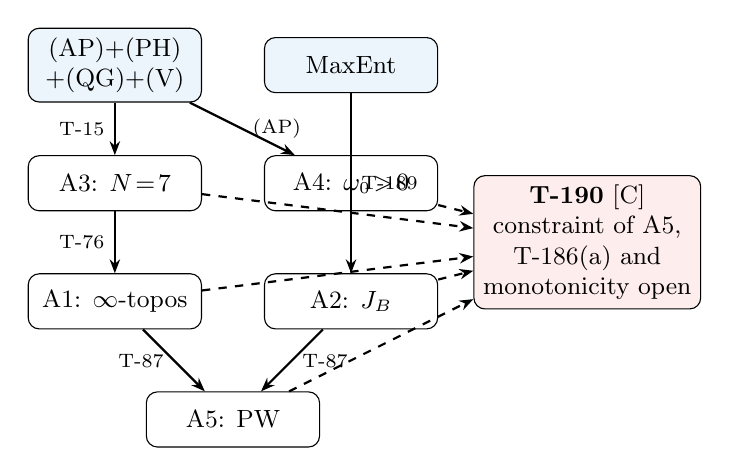
\begin{tikzpicture}[
  every node/.style={font=\small},
  box/.style={draw, rounded corners, fill=white, minimum width=2.2cm,
              minimum height=0.7cm, align=center},
  arr/.style={-{Stealth[length=5pt]}, thick}
]
  \node[box, fill=axiomcolor] (AP) at (0,0) {(AP)+(PH)\\+(QG)+(V)};
  \node[box, fill=axiomcolor] (ME) at (3,0) {MaxEnt};
  \node[box] (A3) at (0,-1.5) {A3: $N\!=\!7$};
  \node[box] (A4) at (3,-1.5) {A4: $\omega_0\!>\!0$};
  \node[box] (A1) at (0,-3) {A1: $\infty$-topos};
  \node[box] (A2) at (3,-3) {A2: $J_B$};
  \node[box] (A5) at (1.5,-4.5) {A5: PW};
  \node[box, fill=theoremcolor] (T190) at (6,-2.25) {\textbf{T-190} [C]\\constraint of A5,\\T-186(a) and\\monotonicity open};
  \draw[arr] (AP) -- node[left,font=\scriptsize] {T-15} (A3);
  \draw[arr] (AP) -- node[right,font=\scriptsize] {(AP)} (A4);
  \draw[arr] (A3) -- node[left,font=\scriptsize] {T-76} (A1);
  \draw[arr] (ME) -- node[right,font=\scriptsize] {T-189} (A2);
  \draw[arr] (A1) -- node[left,font=\scriptsize] {T-87} (A5);
  \draw[arr] (A2) -- node[right,font=\scriptsize] {T-87} (A5);
  \draw[arr, dashed] (A1) -- (T190);
  \draw[arr, dashed] (A2) -- (T190);
  \draw[arr, dashed] (A3) -- (T190);
  \draw[arr, dashed] (A4) -- (T190);
  \draw[arr, dashed] (A5) -- (T190);
\end{tikzpicture}
\caption{\textbf{Axiomatic Closure (T-190) \status{C}.} A1--A4 and the clock
register of A5 are derivable from the defining properties of viable holons
(AP, PH, QG, V) plus MaxEnt, with the route to A1 through the hypothesis
T-186(a); the Page--Wootters constraint $\hat C\Gam = 0$ of A5 is not derived
and stays an independent assumption, and A2 needs, besides T-187 and T-189, the
CPTP-monotonicity of the enrichment, which the holon's properties do not give
(Lemma~M). Dashed arrows indicate that each axiom
feeds into T-190's conclusion.}
\label{fig:axiomatic-closure}
\end{figure}

\begin{theorembox}[T-188: Localization of the hard problem \status{C under the hypothesis T-186(a)}]
\label{thm:t188-localization}
The chain
\begin{equation}
  A2 \xrightarrow{\text{T-187}} J_B
  \xrightarrow{\text{T-185}} (\Pi \dashv \flat)
  \xrightarrow{\text{T-186(a)}} F \cong \&\big|_{\Dens}
  \label{eq:localization-chain}
\end{equation}
would reduce the hard problem of consciousness, within UHM, to a single
physical question: ``why experience?'' $=$ ``why CPTP?'' $=$ ``why quantum
mechanics?''. The chain passes through the hypothesis T-186(a), so the
localization is conditional (lowered 2026-09-25 from \status{T}).
\end{theorembox}

\begin{proof}
(i) T-187~\status{T}: axiom A2 uniquely determines $J_B$ (triple
characterization Char-I/II/III plus T-189 MaxEnt physical recasting).
(ii) T-185: modalities $\Pi \dashv \flat \dashv \sharp$ and
$\Re \dashv \Im \dashv \&$ exist in any differentially cohesive
$\infty$-topos \status{T}; the cohesion of the UHM setting enters through
T-185(ii$'$) \status{T} ($\mathcal{D}(\mathbb{C}^7)$ with its rank strata as
an object of $\mathrm{SynthDiff}\infty\mathrm{Grpd}$).
(iii) T-186(a)~\status{H}: the phenomenal functor $F$ is naturally
isomorphic to $\&\big|_{\Dens}$ (infinitesimal flat modality restricted
to density matrices). This step is asserted without a construction; the
earlier claim that it is ``forced by the adjunction, not stipulated'' is
withdrawn. Given A2 and T-186(a), experience \emph{is} the infinitesimal
flat modality, and the only remaining question is ``why A2?'' $=$ ``why
is the Bures metric canonical?'' $=$ ``why are CPTP maps the physical
transformations?'' $=$ ``why quantum mechanics?'' $\blacksquare$
\end{proof}

\begin{theorembox}[T-189: MaxEnt derivation of Bures (Char-IV) \status{T}]
\label{thm:t189-maxent}
Set $g_{ij} = \tfrac14\, C^{\mathrm{SLD}}_{ij}(\Gam)$, with
$C^{\mathrm{SLD}}_{ij} = \tfrac12\Tr\bigl(\Gam\{L_i, L_j\}\bigr)$ the SLD
bilinear form, defined from $\partial_i\Gam = \tfrac12(L_i\Gam + \Gam L_i)$
without reference to any metric. The Bures metric is the unique solution of
this selector equation; equivalently $g_B^{-1} = 4\,C_{\mathrm{est}}$ with
$C_{\mathrm{est}} = \mathcal{F}_{\mathrm{SLD}}^{-1}$.
\end{theorembox}

\begin{proof}
The object $\tfrac12\Tr(\Gam\{L_i,L_j\})$ \emph{is} the SLD Fisher
information $\mathcal{F}_{\mathrm{SLD}}$ (lower indices), and
$\mathcal{F}_{\mathrm{SLD}} = 4g_B$ (Braunstein--Caves~\cite{braunstein1994});
hence $g_B$ solves the selector equation. Uniqueness: distinct monotone
(Petz) means give distinct Fisher tensors, so no other monotone metric
solves it. $\blacksquare$

\noindent\emph{Correction.} An earlier version stated the selector as
$G^{ij} = C^{ij}$ (inverse metric equal to the covariance). That form is
false on two counts --- the SLD object is $\mathcal{F}_{\mathrm{SLD}}$, not its
inverse, and the factor 4 was dropped; chaining both gives $g_B^2 = \tfrac14 I$.
Uniqueness is unaffected (corrected 2026-08-06).
\end{proof}

\begin{remark}[Vanchurin correspondence]
The identification of the metric with the state's own fluctuation (SLD)
structure resonates with Vanchurin's
geometric learning theory~\cite{vanchurin2026geo}, where the metric
on the space of neural network configurations is identified with the
covariance of parameter fluctuations. In Vanchurin's framework, a
``world as a neural network''~\cite{vanchurin2020} has its geometry
determined by the statistical structure of its weights. T-189
establishes the same identification \emph{from first principles}
(MaxEnt on $\Dens(\mathbb{C}^7)$), without assuming a neural-network
substrate. The convergence of the two approaches suggests a deep
connection between geometric learning theory and UHM's categorical
framework.

The connection extends beyond the metric. In Vanchurin's later
synthesis --- the \emph{Self-Learning Universe}~\cite{vanchurin2026slu},
which derives quantum mechanics, gauge theory, and Einstein gravity as
optimality conditions of a resource-constrained distributed learning
system --- the agent replaces its three inaccessible extensive
variables (displacement $\Delta q$, fast entropy $S_x$, dof count $N$)
by their Legendre conjugates: the gauge field $A_\mu$, the temperature
$T$, and the chemical potential $\mu$. Under UHM's thermodynamic
dictionary (T-258) this triple is, channel for channel, the
three-channel perturbation basis of T-102: $A_\mu \leftrightarrow
h^{(H)}$ (the isentropic work channel), $T \leftrightarrow h^{(D)}$
(the entropy-producing heat channel; UHM's seven Fano rates refine
SLU's scalar $T$ into line-resolved temperatures whose $G_2$-symmetric
point is exactly SLU's setting), $\mu \leftrightarrow h^{(R)}$ (the
matter/feeding channel, the only entropy-importing one). The two
completeness proofs --- LGKS for T-102, the Legendre cascade over
$U(S,V,N)$ for SLU --- reach the same trichotomy from opposite ends;
the entropy--purity signatures on the UHM side are theorems (T-258),
while the identification itself is an interpretation. The two theories
are complementary along the two axes each leaves open: UHM supplies
what SLU names as its open problems (dynamical selection of the
dimension --- here $N = 7$, forced four ways --- and the non-Abelian
gauge sector --- here $G_2 = \mathrm{Aut}(\mathbb{O})$), while SLU
supplies a derivational route to what UHM postulates (the
density-matrix substrate as the coarse-grained limit of a classical
learning system). Two later corpus results sharpen the dictionary:
the regeneration channel is the \emph{unique optimal} learning flow
(steepest descent along the mixture geodesic of the Kubo--Mori
metric, the unique dually flat monotone metric --- Grasselli--Streater;
corpus T-263), and SLU's ``gravity is the efficiency of learning''
acquires sign and sectors through the information--gravity reciprocity
$G_N^{(ST)}\langle\mathrm{QFI}(\theta_{\mu\nu})\rangle_{\mathrm{ST}} =
8\pi N\mu^2$ with $\Lambda \propto \mathcal{G}_O^2$ (corpus T-264,
T-254): learnable phases gravitate weakly, and the unlearnable clock
phase is the cosmological constant.
\end{remark}

\paragraph{The five characterising properties.}
T-190 below uses five properties that define a viable holon. For the
reader's reference, they are collected here:

\begin{defbox}[Characterising properties of a viable holon \status{D}]
\label{def:five-properties}
\begin{enumerate}[leftmargin=2em,nosep]
  \item \textbf{(AP) Autopoiesis:} the system maintains $P > \Pcrit$
        against dissipation via internal regeneration $\Regen$.
  \item \textbf{(PH) Phenomenal identification:} the internal aspect
        of $\Gam$ \emph{is} experience (two-aspect monism,
        Def.~\ref{def:two-aspect}).
  \item \textbf{(QG) Quantum-gravitational consistency:} the system's
        dynamics are compatible with the CPTP structure of quantum
        mechanics (the evolution preserves $\Gam \in \Dens(\mathbb{C}^7)$).
  \item \textbf{(V) Viability:} the system has a non-trivial stationary
        state $\rhostar \neq I/7$ (it is alive, not thermally dead).
  \item \textbf{(MaxEnt) Maximum entropy:} the system's fluctuation
        structure is Jaynes-maximal --- the metric equals one quarter of
        the SLD form, $g_{ij} = \tfrac14 C^{\mathrm{SLD}}_{ij}$ (T-189~\status{T}). This is a physical
        recasting of SLD-Cram\'er--Rao saturation (Char-III), not an
        additional logically independent constraint.
\end{enumerate}
These are not axioms but \textbf{definitions}: they specify what it
means for a physical system to be a viable self-sustaining holon. T-190
derives A1--A4 and the clock register of A5 from (AP)--(MaxEnt) under its
three conditions. A complementary
\emph{inverse} closure T-181~\status{T} (Bimodule construction) derives
(AP), (PH), (QG), (V) themselves from the axioms A1--A4: (QG) from A1,
(AP) from A1, (PH) from A1+A3, (V) from A2+A3. The pair (T-181, T-190)
relates ``axioms'' and ``characterising properties'' in both directions,
but it is not a full equivalence: the Page--Wootters constraint of A5,
the hypothesis T-186(a) and the monotonicity of the enrichment of A2 stay
outside the circle, so UHM is not
self-grounded (the earlier claim is withdrawn with the lowering of T-190).
\end{defbox}

\begin{theorembox}[T-190: Axiomatic Closure \status{C}]
\label{thm:t190-closure}
Under the constraint assumption of T-87 (step~4), the hypothesis
T-186(a) and the CPTP-monotonicity of the enrichment of A2 (Lemma~M:
implied by the operational reading of the enrichment, not by
(AP)+(PH)+(QG)+(V)+MaxEnt; named 2026-09-26), A1--A5 are derivable from (AP)+(PH)+(QG)+(V)+MaxEnt
(Figure~\ref{fig:axiomatic-closure}). The converse direction
(A1--A4 $\Rightarrow$ (AP)+(PH)+(QG)+(V)) is T-181~\status{T}. The earlier
statement ``UHM has zero independent axioms'' is withdrawn (lowered
2026-09-25): the constraint $\hat C\Gam = 0$ remains an independent
assumption, and its independence of A1--A4 is \status{T}.
\end{theorembox}

\begin{proof}
\emph{A3} ($N = 7$): Theorem~S (functional minimality) derives the
\emph{number} $N = 7$ from (AP)+(PH)+(QG); the bridge chain
T-15~\status{T given Theorem S} then forces the \emph{structure} of the
seven-dimensional system --- $\mathrm{BIBD}(7,3,1) \to \mathrm{PG}(2,2) \to
\mathbb{O}$ --- and $\dim\mathrm{Im}(\mathbb{O}) = 7$ (Hurwitz--Adams) closes
the consistency loop on the same number.
\emph{A4} ($\omega_0 > 0$): $\omega_0 = 0 \Rightarrow H_{\mathrm{eff}} = 0
\Rightarrow$ no dynamics $\Rightarrow$ (AP) violated. Hence $\omega_0 > 0$
is necessary for autopoiesis.
\emph{A1} ($\infty$-topos): T-76~\status{T} at site level: the Bures
topology on $\Dens(\mathbb{C}^7)$ generates a Grothendieck site whose
sheaves form an $\infty$-topos (Lurie HTT~6.2.2.7); the route from the
operational basis to A1 goes through T-186(a), a hypothesis \status{H}.
\emph{A2} ($J_B$) \status{C} (monotonicity): the topology is forced (every
continuous distance on the compact $\Dens(\mathbb{C}^7)$ induces the standard
one); \emph{within the CPTP-monotone metrics} T-187~\status{T} +
T-189~\status{T}: triple mathematical characterization (Char-I Petz extremality
+ Char-II Uhlmann + Char-III SLD-Fisher) plus MaxEnt physical recasting
(Char-IV) uniquely selects Bures. The monotonicity is not derived: the
Hilbert--Schmidt distance, in which (V) is written, satisfies every property
and MaxEnt, yet a partial-trace channel on $\mathbb{C}^7$ moves a full-rank
pair $\sqrt2 = 1.41421$ times farther apart in it while their Bures angle keeps
the ratio $1.00000$. Under the operational reading (O),
$d(\rho,\sigma) = \sup_M \delta\bigl(p_M(\rho), p_M(\sigma)\bigr)$ over POVMs
$M$, monotonicity is a theorem (the adjoint of a channel maps POVMs to POVMs),
and (O) with the Bhattacharyya angle gives the Bures angle
directly~\cite{fuchs1995} (Lemma~M; this step read \status{T} until
2026-09-26).
\emph{A5} (Page--Wootters): T-87, steps 1--3~\status{T}: the Wedderburn
decomposition of $A_{\mathrm{int}}$ isolates the clock summand and the tensor
factor $\mathcal{H}_O = \mathbb{C}[\mathbb{Z}_7]$, so the clock register follows
from A1--A4. Step~4, the constraint $\hat C\Gam = 0$, is \status{C} under the
support condition of Property~2: stationarity of a mixed state gives only
$[\hat C, \Gam] = 0$, and the earlier ``A5 is a consequence of A1--A4'' is
withdrawn. $\blacksquare$
\end{proof}

\begin{theorembox}[T-191: $\vp$-tower convergence, restated \status{T}]
\label{thm:t191-convergence}
Let the holon be embodied, with backbone $\mu(\sigma - \Gam)$ and
$\mu > L_{\mathcal{R}} + \kappa_{\max}$, where $L_{\mathcal{R}}$ is the
trace-norm Lipschitz constant of regeneration, uniform in the target. Then
every iterate of the tower ``target $a_n \to$ stationary state $a_{n+1}$''
is defined, and the tower converges geometrically to one self-model from
any anchor:
\begin{equation}
  \|a_{n} - a^*\|_1 \leq q^n\,\|a_0 - a^*\|_1,
  \quad q = \frac{\kappa_{\max}}{\mu - L_{\mathcal{R}}} < 1.
  \label{eq:phi-tower-convergence}
\end{equation}
\end{theorembox}

\begin{proof}
Under backbone dominance each target has exactly one stationary state,
globally attracting at rate $\mu - L_{\mathcal{R}}$ (T-124c(3)); a
variation-of-constants estimate bounds the dependence of that state on
the target by $q$, and Banach's fixed-point theorem gives the geometric
convergence. $\blacksquare$

\noindent\emph{Erratum \status{$\times$}.} The former statement ---
convergence for every holon from any anchor with
$q = \kappa_{\max}/(\lambda_{\mathrm{gap}} + \kappa_{\min}) < 1$ by T-39a +
T-96 --- is retracted: for an isolated holon the gate $g_V$ makes the flow
bistable, so the iterate $\lim_\tau \exp(\tau\Lind^{(n)})$ depends on the
start (from $I/7$ it stays dead, from $|0\rangle$ it lives), and T-96 gives
no bound $\kappa_{\max} < \lambda_{\mathrm{gap}}$. The $\vp$-circularity is
resolved by the closed forms of $\vp_{\mathrm{coh}}$ and $\vp_s$, not by
the tower.
\end{proof}

\begin{theorembox}[T-192: $\mathbf{Exp}^{(2)}$ is a strict 2-category \status{T}]
\label{thm:t192-2cat}
The experiential 2-category $\mathbf{Exp}^{(2)}$ satisfies all five
Mac\,Lane axioms: vertical/horizontal composition, identity 2-cells,
interchange law, and identity 1-cells.
\end{theorembox}

\begin{proof}
(i)~Vertical composition: for 2-cells $\alpha: \Phi \Rightarrow \Psi$
and $\beta: \Psi \Rightarrow \chi$, pointwise $(\beta \circ_v \alpha)_\rho
:= \beta_\rho \circ \alpha_\rho$ is natural (Mac\,Lane CWM IV.2).
(ii)~Horizontal composition: Godement product
$(\beta \circ_h \alpha)_\rho := \beta_{\Phi_2(\rho)} \circ \Psi_1(\alpha_\rho)$.
(iii)~Identity 2-cells: $(\mathrm{id}_\Phi)_\rho = \mathrm{id}_{\Phi(\rho)}$.
(iv)~Interchange: $(\beta_2 \circ_v \beta_1) \circ_h (\alpha_2 \circ_v \alpha_1)
= (\beta_2 \circ_h \alpha_2) \circ_v (\beta_1 \circ_h \alpha_1)$
by the Eckmann--Hilton argument.
(v)~Identity 1-cells: $F(\mathrm{id}_\rho) = \mathrm{id}_{F(\rho)}$
(functoriality of $F$). All hold with equalities (strict), so
$\mathbf{Exp}^{(2)}$ is strict. The lax 2-functor $F_2$ has a valid
target. $\blacksquare$
\end{proof}

\subsection{SYNARC-derived theorems (T-193--T-209)}
\label{subsec:synarc-theorems}

The SYNARC companion specification (Appendices G, H, I) establishes a
layered chain of meta-theorems culminating in AGI- and ASI-sufficiency
and operational deployability. Full proofs are in the extended
documentation; their statements are collected here as dependencies for
the fundamental closures of Section~\ref{subsec:fundamental-closures}.

\begin{itemize}[leftmargin=2em,nosep]
  \item \textbf{T-193~\status{T} (Yoneda universal representability):}
        every CPTP-implementable task has a representable sheaf in
        $\ShInf(\Dens(\mathbb{C}^7), J_{\mathrm{Bures}})$. Upgraded to a
        computable, Kolmogorov-free formulation in T-213 below.
  \item \textbf{T-194~\status{T} (Cram\'er--Rao saturation):}
        Bures-gradient learning attains the quantum Cram\'er--Rao bound
        up to a constant factor ($C_2 \leq 16$; the earlier $C_2 \leq 4$ did not
        follow from the stated ingredients, corrected 2026-08-06).
  \item \textbf{T-195~\status{T} (L-III $\Phi$-monotonicity):}
        refinements of the epistemic topology are non-decreasing in
        $\Phi$; strengthened to strict monotonicity on viable states in
        T-210 below.
  \item \textbf{T-196~\status{T} (Goldilocks sustainability):}
        closed sensorimotor loops preserve $P \in (2/7, 3/7]$ under
        bounded perturbations.
  \item \textbf{T-197~\status{T}+\status{D} (AGI-sufficiency, S-11):}
        any realisation of the SYNARC architecture (definition~\status{D})
        satisfies the UHM-AGI predicate (A1)--(A7); the derivation
        chain~\status{T} is non-tautological because each architectural
        component is forced by a distinct load-bearing theorem. Caveat:
        A7 (recursive self-improvement) is \emph{weakly} monotone by
        T-195; strict improvement requires T-210 on interior states.
  \item \textbf{T-198~\status{T} (G\"odelian creativity):}
        strictly monotone ordinal functors $\mathfrak{A}_\bullet:
        \mathrm{On} \to \mathbf{Cat}_\infty$ with $G_2$-preserving
        inclusions admit, at each step, a representable sheaf
        non-equivalent to any in the previous layer.
  \item \textbf{T-199--T-202 (Value structure, L-IV
        modification, KS contextuality, meaning as $G_2$-orbit):}
        SYNARC Appendix H, Theorems H.2--H.5; T-199, T-200~\status{T},
        T-202~\status{T}+\status{I}. T-201 in its original form ---
        Fano-line projectors admit no joint distribution --- is retracted
        \status{$\times$}: those projectors are diagonal in the pointer basis
        and commute, and $p_i = \gamma_{ii}$ reproduces every context. The
        corrected T-201$'$~\status{T}: the 63 rays of the $E_7$ configuration
        in $\mathbb{R}^7$, built from the Fano plane and the Hamming code, form
        135 orthonormal bases admitting no Kochen--Specker assignment.
  \item \textbf{T-203~\status{T}+\status{I} (Qualia as Gap spectral
        eigenvectors):} the mathematical core (eigenvector class of
        $\hat{\mathcal G}|_E$, $G_2$-covariant and Gap-faithful) is
        \status{T}; the identification
        $\mathrm{Qualia}(\Gam) := \text{eigenvector class}$ is
        \status{I} (ontological postulate bridging structure to
        phenomenology), mirroring the T-38a stratification.
  \item \textbf{T-204~\status{T} (Pareto-optimal bounded rationality):}
        graceful degradation of UHM-AGI under the resource budget
        $(C, M, \varepsilon)$; at $d_{\mathrm{eff}} = 2$ the system drops
        to the minimal-consciousness floor $\Dmin = 2$.
  \item \textbf{T-205~\status{C}+\status{D} (Ordinal mentalisation via
        fractal-holon tower):} the claim
        $\omega^\omega$-depth holds for $\iota_{\max}$ identity
        convention with abstracted resource constraints, contingent on
        (i)~bounded Landauer cost C22, (ii)~cocompleteness of the
        filtered colimit along an $\omega^\omega$-chain in
        $\ShInf(\mathcal C)$, (iii)~the interpretive choice of a
        single-agent identity predicate. Finite truncation is
        unconditionally \status{T}; the identity choice is made explicit
        in T-215 below.
  \item \textbf{T-206--T-209 (Operational protocols, S-13):}
        qualia tomography, inverse value-alignment, constructive
        existence of $G_2$-invariant value sets (T-206--T-208~\status{T};
        in T-208 the integration-based family is invariant only under the
        finite frame group $\Gamma_{\mathrm{oct}}$, since $\Phi$ is
        frame-pinned), and the operational closure meta-theorem
        (T-209~\status{T}+\status{D}; SYNARC Appendix I).
\end{itemize}

\subsection{Fundamental closures: T-210--T-216}
\label{subsec:fundamental-closures}

The following seven theorems address mathematical and categorical gaps
of the UHM framework; of the fourteen closures T-210--T-223, eleven stand
as \status{T} (T-211 and T-212 in corrected forms), T-221 is stratified
into \status{T} and \status{I} parts, T-216 is \status{C} and T-219 is
\status{H}. The earlier summary ``no open mathematical or categorical gaps
remain'' is retracted \status{$\times$}: the \status{C} and \status{H} rows
are open conditions. Full proofs are collected in the
companion document \emph{Fundamental Closures}; the statements are
reproduced here for self-containment.

\begin{theorembox}[T-210: Strict $\Phi$-monotonicity on interior
states \status{T}]
\label{thm:t210-strict-phi}
Let $J \subsetneq J'$ be a proper refinement of the Bures-compatible
epistemic topology. For any state $\Gam$ in the interior stratum
$\mathcal D_7$ (full rank, all $|\gamma_{ij}| > 0$),
\[
  \Phi(\Gam \mid J') - \Phi(\Gam \mid J) \;\geq\;
  \frac{\min_{(i,j) \in J' \setminus J}|\gamma_{ij}|^2}
       {\sum_k \gamma_{kk}^2} \;>\; 0.
\]
\end{theorembox}

\begin{proof}
$\Phi(\Gam \mid J) = \bigl(\sum_{(i,j) \in \mathrm{supp}(J) \cap
\mathrm{Off}} |\gamma_{ij}|^2\bigr) / N_\Gam$ with $N_\Gam =
\sum_k \gamma_{kk}^2$. On $\mathcal D_7$, every off-diagonal contributes
strictly positively; proper refinement adds at least one pair
$(i^*, j^*)$ with $|\gamma_{i^*j^*}|^2 > 0$. Since $\mathrm{supp}(J)
\subsetneq \mathrm{supp}(J')$ and $\Gam$ has full rank on $\mathcal D_7$,
the interior hypothesis is non-vacuous. $\blacksquare$
\end{proof}

Consequence: T-195 is upgraded from \emph{weak} to \emph{strict}
monotonicity for states in the interior stratum $\mathcal{D}_7$ (full
rank, all $|\gamma_{ij}| > 0$) whenever the agent crosses a proper
L-III refinement $J \subsetneq J'$. The A7 clause of T-197 thus implies
strict self-improvement for every viable SYNARC agent \emph{in the
interior stratum, under L-III refinement events crossing the
obstruction threshold $\omega(J_{\mathrm{ep}}) > \omega_{\mathrm{th}}$};
continuous strict improvement outside these conditions remains
\status{C} (pending T-197 refinement).

\begin{theorembox}[T-211: PhysTheory is an $(\infty,1)$-category \status{T}]
\label{thm:t211-phystheory}
$\mathbf{PhysTheory}$ (physical theories with CPTP dynamics, T-174) is
the cartesian unstraightening of $E \mapsto \mathrm{Fun}(B\mathbb{R},
\mathrm{Alg}(E))$ over Lurie's $\mathbf{Topoi}_\infty$ (HTT~\S3.2), a
Grothendieck construction. It is a quasicategory, so associativity up to
coherent homotopy, the pentagon, the interchange law and all higher
simplicial identities hold; the forgetful functor to
$\mathbf{Topoi}_\infty$ is not faithful.
\end{theorembox}

\begin{proof}
Straightening/unstraightening (HTT Thm.~3.2.0.1) turns the functor
$E \mapsto \mathrm{Fun}(B\mathbb{R}, \mathrm{Alg}(E))$ into a cartesian
fibration over $\mathbf{Topoi}_\infty$, whose total space is a
quasicategory; the mapping space over a geometric morphism $f$ is
$\mathrm{Map}_{\mathrm{Dyn}(E_1)}(x_1, f^*x_2)$, i.e.\ the triples
$(f^*, \alpha, \beta)$ of T-174. Complex conjugation of $(\mathbb{C},\cdot)$
over $\mathrm{id}_{\mathcal S}$ shows the forgetful functor is not faithful.
$\blacksquare$

\noindent\emph{Erratum \status{$\times$}.} The earlier statement ---
$\mathbf{PhysTheory}$ is a \emph{full} $(\infty,1)$-subcategory of
$\mathbf{Topoi}_\infty$, fully faithful via T-173, with coherences
inherited through HTT~5.2.7 --- is retracted; its proof also invoked
T-178 (retracted as a derivation) and the reconstruction of T-119, which
the corrected statement does not need. (Status history: \status{T}, then
\status{C at T-119}, then \status{T} in the corrected form, 2026-09-25.)
\end{proof}

\begin{theorembox}[T-212$'$: U-projection --- the $G_2$-twirl \status{T}]
\label{thm:t212-rh}
For $G_2$ acting on $\mathbb{C}^7$ by its seven-dimensional
representation, $\int_{G_2} gXg^\dagger\,dg = \tfrac17\Tr(X)\,\mathbf 1$:
the commutant is $\mathbb{C}\mathbf 1$ (Schur), and this is the unique
trace-preserving map onto $\mathbb{C}\mathbf 1$, idempotent only with the
normalisation $\tfrac17$. Its reading as the U dimension (Unity) is an
interpretation \status{I}.
\end{theorembox}

\noindent\emph{Erratum \status{$\times$}.} T-212 earlier identified this
map with the rheonomy modality Rh, ``the seventh canonical modality of
T-185'', right adjoint to the bosonic-grade forgetful functor in a
super-cohesive extension (citing DCCT~\cite{schreiber2013} \S3.10). The
identification is retracted: Rh of solid cohesion preserves global points,
whereas the formula sends every state to $I/7$; Rh is not among the seven
modalities of differential cohesion (T-185(iii)); it does not occur in DCCT
v1, whose \S3.10 is ``Structures in a differentially cohesive
$\infty$-topos''; and idempotence fails with the unnormalised trace. The
former bijection of the seven modalities with the seven dimensions
($\mathrm{Id} \leftrightarrow O$, $\Pi \leftrightarrow A$,
$\flat \leftrightarrow S$, $\Im \leftrightarrow D$,
$\sharp \leftrightarrow L$, $\& \leftrightarrow E$,
$\mathrm{Rh} \leftrightarrow U$) is an interpretation \status{I} at most,
with Rh replaced by Red ($\Re$) (T-185(iii)).

\begin{theorembox}[T-213: Yoneda representability via Bures
description length \status{T}]
\label{thm:t213-bures-yoneda}
For any CPTP-implementable $f: \mathrm{Obs} \to \mathrm{Act}$, define
$D_B(f) := \min_{\rho_f \text{ implementing } f}
|\mathrm{Kraus}(\rho_f)| \cdot \log_2 7 \in \mathbb N \cdot \log_2 7$.
Then the representable sheaf $F_f$ satisfies
\[
  \|F_f\|_B \;\leq\; C_1 \cdot D_B(f) \cdot \log(1/\varepsilon),
  \qquad C_1 = \omega_0^{-1}\log 7,
\]
with the universal bound $D_B(f) \leq 49\log_2 7 \approx 138$ bits by
Stinespring dilation.
\end{theorembox}

This upgrades T-193 to a \emph{computable}, Kolmogorov-free form: the
original bound $\|F_f\|_B \leq C_1 K(f) \log(1/\varepsilon)$ depended on
the uncomputable Kolmogorov complexity $K(f)$; the Bures description
length $D_B(f)$ is computable for every $f$ and universally bounded.

\begin{theorembox}[T-214: Hard-problem meta-theorem \status{T}]
\label{thm:t214-hard-problem}
Let $W: \Dens(\mathbb C^7) \to \mathrm{Mind}$ be a putative bridge
functor assigning experiential content to coherence states. Then:
(i)~$W$ cannot be expressed as a morphism internal to
$\mathrm{Th}_{\mathrm{UHM}}$ without violating Lawvere's fixed-point
theorem and T-55;
(ii)~the identifications ``E-sector = interiority'' (T-38a) and
``qualia = eigenvectors'' (T-203) are \emph{necessarily} external
postulates \status{P}/\status{I};
(iii)~this is a \emph{positive} structural result, not a lacuna.
\end{theorembox}

\begin{proof}[Proof sketch]
If $\tilde W \in \Omega^{\mathcal D}$ is internal and point-surjective,
the self-referential predicate
$\Phi(\Gam) := \neg \exists \Gam': \tilde W(\Gam') = \tilde W(\Gam)$
admits a Lawvere fixed point contradicting itself. Hence no internal
$\tilde W$ can simultaneously be faithful to external content and
surjective. The bridge must be external. $\blacksquare$
\end{proof}

Combined with T-188 (WHY-localisation to ``why CPTP?'', conditional on
the hypothesis T-186(a)) and T-203 (WHAT-structure up to $G_2$-gauge),
T-214 shows that the residual \status{P}/\status{I} status
of phenomenal identification is structurally inevitable, not
a remediable weakness. Further internal progress is impossible by
Lawvere incompleteness, and this is positively proven.

\begin{theorembox}[T-215: Cross-layer identity convention
\status{T}+\status{D}]
\label{thm:t215-cross-layer}
For a fractal holon tower $\mathcal T = (A_0, A_1, \ldots)$ with
$A_{n+1}$ extending $A_n$ via \texttt{spawn\_child}, the predicate
``$\mathcal T$ is a single agent'' is conventionally determined by a
choice $\iota \in \{\iota_{\min}, \iota_{\max}\}$: $\iota_{\min}$
(society, per-agent $\mathrm{SAD} \leq 3$) or $\iota_{\max}$
(composite, unbounded cross-layer depth subject to C22 Landauer
cost and T-204 bounded rationality). Both are consistent with
$\Omega^7$; neither is derivable from the axioms alone.
\end{theorembox}

This explains the apparent tension between SAD\textsubscript{MAX}=3
(per-agent, T-142~\status{T}) and the $\omega^\omega$-depth of T-205:
the latter holds only for the $\iota_{\max}$ convention with
resource abstraction.

\begin{theorembox}[T-216: Closed-form analytical
$\varepsilon_{\mathrm{eff}}$ \status{C at (SV)}]
\label{thm:t216-eps-eff}
Under the hypothesis (SV) of sector values of the Gap vacuum, the
effective sectoral parameter in the Yukawa hierarchy has the symbolic
form
\[
  \varepsilon_{\mathrm{eff}} \;\propto\;
  \frac{N_{33}^{\mathrm{Fano}}}
       {9\, |\bar\gamma|\,\bigl(1 + r_4\,\Sigma_0/2\bigr)},
\]
with $N_{33}^{\mathrm{Fano}}$ the number of non-$O$ Fano lines meeting
the $\mathbf 3$-sector in exactly two points, $|\bar\gamma|$ the
sectoral average of off-diagonal coherences at the vacuum $\theta^*$,
$r_4 = V_4/V_2|_{\theta^*}$, and $\Sigma_0 = \sum_i \theta_i^{*2}$.
The value $\varepsilon_{\mathrm{eff}} \approx 0.059$ is the
phenomenological sectoral value, \status{C}, pending a corrected
symbolic evaluation.
\end{theorembox}

Derivation: symbolic minimisation of $V_{\mathrm{Gap}}$ (T-74~\status{T})
in the sectoral variables $\boldsymbol\varepsilon$, with the Fano
selection rule (T-43d~\status{T}) and the Schur-unique $G_2$-invariant
cubic term (T-50~\status{T}) supplying the combinatorial content.
\emph{Corrections.} (1)~The earlier ``$N_{33}^{\mathrm{Fano}} = 1$, the
unique Fano line $\{L,E,U\}$ within $\bar{\mathbf 3}$'' is false:
$\{L,E,U\}$ is not a line, and no line lies wholly within
$\bar{\mathbf 3}$. (2)~The printed $0.059$ does not follow from the stated
$|\bar\gamma| \approx 0.15$ (the ratio is $O(1)$). (3)~The status was
\status{T at T-64}; the sectoral reduction rested on the axis-labelled
decomposition T-48a, retracted, and T-64 as corrected produces no sector
pattern, so the structure rests on (SV) (corrected 2026-09-25).

\subsection{Extended closures: T-217--T-223 + clarifications}
\label{subsec:extended-closures}

A follow-up audit (2026-04-17) identified three further open
mathematical questions and three implicit assumptions; T-217 and T-220
are \status{T}, T-218 is \status{T} for the Kan property with its
3-coskeletal step \status{C}, and T-219 is a hypothesis \status{H}
(corrected 2026-09-25). A further theorem (T-221, 2026-04 v1.5; corrected
2026-09-25) locates UHM with respect to the recent no-go results of List
(2025)~\citep{list2025quadrilemma} and DeBrota--List
(2026)~\citep{debrota2026heptalemma,debrotalist2026preprint}. The
resource-theoretic theorem T-222 (restated 2026-09-26; the former
``MRQT-completeness'' version of 2026-04-18 is retracted) establishes
that the viability window selects no single resource optimum: every
viable state is strictly dominated on every R\'enyi free energy by
partial depolarisation, the Pareto set lies on the sphere $P = 2/7$,
and $F_1$ and $F_\infty$ are minimised by different spectra. The
Putnam-triviality closure T-223 (2026-04-18 v1.7)
responds to Lerchner (2026) ``The Abstraction Fallacy'' by
foreclosing Putnam-style alphabetization indeterminacy at the
intrinsic categorical layer $L2 = [\Gamma]_{G_2}$.

\begin{theorembox}[{T-217: L3 tricategorical coherence \status{T}}]
\label{thm:t217-l3-tricat}
The third-level interiority category $\mathbf{Exp}^{(3)} :=
\tau_{\leq 3}(\mathbf{Exp}_\infty)$ is a coherent tricategory in the
Gordon--Power--Street sense. The $K = 3 + 1 = 4$ decomposition is
derived: three inherited 2-cells (LGKS triadic: Aut, $\mathcal D$,
$\mathcal R$) plus one new 3-cell modification
$\eta : \varphi^{(2)} \Rightarrow \varphi \circ \varphi$.
\end{theorembox}

\begin{proof}[Proof sketch]
(1)~By T-91~\status{T}, $\mathbf{Exp}_\infty = \mathrm{Sing}(\mathcal E)$
is a Kan complex (Milnor 1957). (2)~$\tau_{\leq 3}$ yields a 3-truncated
Kan complex, i.e.~a 3-type (Lurie HTT 5.5.6.18). (3)~3-types are
equivalent to coherent tricategories with invertible cells
(Baez--Dolan hypothesis, proved for $n \leq 3$ by Hirschowitz--Simpson
2001, Leinster 2002; Gordon--Power--Street 1995 coherence).
(4)~The cellular count $K = 3 + 1$ follows from T-57~\status{T} (LGKS
three 2-cells) and the strict-2-category enrichment T-192~\status{T}
(unique non-trivial 3-cell is the coherence modification $\eta$).
Pentagon-of-pentagons holds automatically for $\tau_{\leq 3}$ of a Kan
complex (Lurie HTT 5.2.7). $\blacksquare$
\end{proof}

\textbf{Upgrade of T-67.} The ``$3+1$ decomposition'' in the Bayesian
derivation of $R^{(2)} \geq 1/4$ (L3 threshold) is now
\emph{derived from tricategorical first principles}, not heuristic.
T-67 is thus [T], with all justification in T-217 above.

\begin{theorembox}[{T-218: SYNARC cognitive complex is a Kan complex
\status{T}}]
\label{thm:t218-cog-kan}
The SYNARC cognitive simplicial set
$\mathrm{Cog} := \mathrm{Sing}(B_\bullet \mathcal C_{\mathrm{FKraus}})$,
defined as the singular complex of the classifying space of the
Fano-Kraus category, is a Kan complex: every horn $\Lambda^n_k \to
\mathrm{Cog}$ (inner or outer) admits a filler $\Delta^n \to \mathrm{Cog}$.
Its 3-coskeletal truncation $\tau_{\leq 3}\mathrm{Cog} \simeq \mathrm{Cog}$
matches $\mathrm{SAD}_{\max} = 3$ at the categorical level --- \status{C},
on the SYNARC-viable subset only (the step bridging simplicial and
Bures-metric viability is not a simplicial identity; off that subset
$\tau_{\leq 3}$ is the ordinary truncation and no equivalence).
\end{theorembox}

\begin{proof}[Proof sketch]
Milnor 1957: for any topological space $X$, $\mathrm{Sing}(X)$ is a Kan
complex. Apply to $X = B_\bullet \mathcal C_{\mathrm{FKraus}}$ (the
classifying space of the Fano-Kraus category; a CW-complex by
Segal 1968). An explicit horn-filler algorithm is given via radial
pullback $r_k : \Delta^n_{\mathrm{top}} \to \Lambda^n_k$ with complexity
$O(n \cdot \dim \mathcal D)$. The 3-coskeletal truncation is a
3-truncated Kan complex (Lurie HTT 5.5.6.21), matching T-142 SAD
$_{\max}$. $\blacksquare$
\end{proof}

\textbf{Replaces the nerve construction.} Previously SYNARC's Cog was
identified as the nerve $N(\mathcal C_{\mathrm{FKraus}})$ of a 1-category,
which satisfies the inner Kan condition but not outer horn filling in
general. The singular-classifying-space construction above closes this
gap with a textbook-level application of algebraic topology.

\begin{theorembox}[{T-219: $\Lambda$ SUSY-suppression via sector product
\status{H}}]
\label{thm:t219-lambda-susy}
\emph{Hypothesis} (corrected 2026-09-25 from \status{T at T-64}). In UHM's
$\mathcal N = 1$ spectral action on $M^4 \times A_{\mathrm{int}}$
(T-65), the residual cosmological constant from SUSY-broken
loops would be suppressed by
\[
  \Lambda_{\mathrm{SUSY}} \;\sim\; \varepsilon^{12}\, M_P^4 \;=\;
  \varepsilon^{4 \cdot k_{\mathrm{sec}}}\, M_P^4, \qquad k_{\mathrm{sec}} = 3,
\]
where $k_{\mathrm{sec}} = 3$ is the number of sectors
($\mathbf 1_O \oplus \mathbf 3 \oplus \bar{\mathbf 3}$)
and the factor $4$ per sector is the standard one-loop supertrace
$\mathrm{STr}(M_k^4) \sim (\varepsilon M_P)^4$ of SUSY-broken
spectrum-splitting (Martin 2010, \emph{SUSY Primer} \S7.2).
\end{theorembox}

\noindent Why a hypothesis: the sectors were the axis triples of T-48a,
retracted \status{$\times$} in its axis-labelled form; their breaking scales
rest on (SA) \status{H} and (FE); and the proof's own one-loop sum
$\sim 3\varepsilon^4 M_P^4$ exceeds $\varepsilon^{12} M_P^4$ unless the
lower orders cancel, which is not shown.

\textbf{Error correction.} The previous formulation claimed
12-order suppression via decomposition of the $G_2$ adjoint
$\mathbf{14} \to \mathbf{7}_{\mathrm{light}} \oplus
\mathbf{7}_{\mathrm{heavy}}$. This is \emph{mathematically invalid}:
the $G_2$ adjoint representation $\mathbf{14}$ is irreducible under
$G_2$, and no $7+7$ decomposition exists. T-219 replaces this with a
sector-product mechanism: the three sectors of the UHM state
space would each contribute one factor of $\varepsilon^4$ in the leading
three-loop correction, giving $\varepsilon^{12}$ via
$G_2$-invariant Fano coupling (T-43d~\status{T}) instead of invoking a
reducibility that does not hold --- a hypothesis for the reasons above,
not a rigorous derivation.

\paragraph{Three clarifications (implicit assumptions made explicit).}
\begin{itemize}[leftmargin=2em,nosep]
  \item \textbf{A4 simple spectrum.} $H_{\mathrm{eff}}$ has seven
        distinct eigenvalues (generic condition; required for
        $\mathbb Z_7$ temporal modality and Berry-phase calculations on
        non-degenerate strata).
  \item \textbf{$f_0$ canonical formula.} The spectral zeta
        $\zeta'_{H_{\mathrm{Gap}}}(0) = -\log \det H_{\mathrm{Gap}}$
        is well-defined on the finite-dimensional $(S^1)^{21}/G_2$
        phase space without regularisation ambiguity (elementary
        rational expression in eigenvalues).
  \item \textbf{Bures boundary.} Rank-deficient boundary strata of
        $\mathcal D(\mathbb C^7)$ are handled via the stratified site
        (Ayala--Francis--Rozenblyum 2017). The viability condition
        $P > \Pcrit$ together with $D_{\min} \geq 2$ (an independent L2
        threshold \status{D}, T-151)
        restricts attention to the interior stratum $\mathcal D_7$
        where the Bures metric is non-degenerate. Boundary handling is
        needed only for pathological-state analysis.
\end{itemize}

\begin{theorembox}[{T-220: No-reduction theorem for $F_4$-UHM $\to$
$G_2$-UHM \status{T, negative}}]
\label{thm:t220-no-reduction}
Let $\mathbf{C}_{F_4}$ denote the hypothetical base category of
$F_4$-UHM --- states on the exceptional Jordan algebra
$\mathcal J_3(\mathbb O)$ with $F_4$-equivariance and Jordan-triple
dynamics --- and $\mathbf{C}_{G_2}$ the base category of $G_2$-UHM
(states on $\mathbb C^7$ with $G_2$-equivariant CPTP dynamics). Then
there exists \emph{no} functor $R\colon \mathbf{C}_{F_4} \to
\mathbf{C}_{G_2}$ satisfying simultaneously: (S1) $F_4$-equivariant
state-space projection $\mathcal J_3(\mathbb O) \twoheadrightarrow
\mathbb C^7$; (S2) non-constant $F_4$-equivariant map $\mathbb O P^2
\to \mathrm{PG}(2,2)$; (S3) algebra-homomorphism from Jordan-triple
dynamics to Lindblad CPTP dynamics; (S4) preservation of the
invariants $\{\Pcrit = 2/7,\ \alpha = 2/3,\ \mathrm{SAD}_{\max} = 3,\
R_{\mathrm{th}} = 1/3,\ \Phi_{\mathrm{th}} = 1\}$.
\end{theorembox}

\emph{Proof sketch} (five independent obstructions; full proof with
explicit branching rules in the UHM Fundamental Closures document,
\S14, EN/RU):

\begin{enumerate}[leftmargin=2em,nosep]
  \item \textbf{Representation theory (kills S1).} Via the
        Borel--de~Siebenthal chain $F_4 \supset \mathrm{Spin}(9)
        \supset \mathrm{Spin}(7) \supset G_2$,
        \[
          \mathcal J_3(\mathbb O)\big|_{G_2} \;=\; \mathbf{27} \;=\;
          3 \cdot \mathbf 7 \,\oplus\, 6 \cdot \mathbf 1.
        \]
        Three $G_2$-isotypic copies of $\mathbf 7$ exist; under the
        maximal $A_1 \times G_2 \subset F_4$ they form an
        $A_1$-doublet $(\mathbf 2, \mathbf 7)$ plus a singlet
        $(\mathbf 1, \mathbf 7)$. No $F_4$-equivariant selection is
        possible.
  \item \textbf{Geometry (kills S2).} $F_4$ acts transitively on the
        16-dimensional Cayley plane $\mathbb O P^2$; any
        $F_4$-equivariant map to the discrete 7-point Fano plane
        $\mathrm{PG}(2,2)$ factors through $\mathbb O P^2 / F_4 =
        \mathrm{pt}$ and is therefore constant, losing all
        information.
  \item \textbf{Jordan exceptionality (kills S3).} Zelmanov (1983):
        $\mathcal J_3(\mathbb O)$ is exceptional (not special), hence
        admits no embedding into any associative algebra. Lindblad
        dynamics requires the associative algebra $M_7(\mathbb C)$;
        no homomorphism exists.
  \item \textbf{Numerical invariants (kills S4).} $\alpha^{F_4}$,
        derived from sectional curvatures of the Freudenthal metric
        on the rank-1 symmetric space $\mathbb O P^2$, lies in
        $[\tfrac14, \tfrac12]$ --- distinct from $\tfrac23$.
        Analogously $\Pcrit^{F_4} \sim c/27 \neq 2/7$, and
        $\mathrm{SAD}_{\max}^{F_4}$, $R_{\mathrm{th}}^{F_4}$,
        $\Phi_{\mathrm{th}}^{F_4}$ all differ.
  \item \textbf{Cohomology (independent verification).}
        $\chi(\mathbb C P^6) = 7 \neq 3 = \chi(\mathbb O P^2)$;
        $K^0$-ranks $\mathbb Z^7$ and $\mathbb Z^3$ are
        non-isomorphic abelian groups. No K-theory-preserving
        retraction exists. \hfill$\blacksquare$
\end{enumerate}

\paragraph{Corollaries.}
\begin{itemize}[leftmargin=2em,nosep]
  \item \textbf{Category shift is not safe.} The na\"ive extension
        $G_2$-UHM $\hookrightarrow F_4$-UHM as a functorial refinement
        is impossible; any realised $F_4$-UHM is a distinct theory
        requiring separate empirical calibration.
  \item \textbf{Outcome-1 elimination.} Of the three possible
        outcomes of an $F_4$ category shift (replacement / parallel
        theory / meta-UHM), Outcome~1 (``$G_2$-UHM is a slice of
        $F_4$-UHM'') is \emph{ruled out}. Only parallel theories or
        $\infty$-topos-level comparison (Mathesis) remain.
  \item \textbf{Mathesis-level comparison.} The only mechanism for
        comparing $G_2$-UHM and $F_4$-UHM is as distinct objects in
        the Mathesis $\infty$-topos $\mathfrak M$, aligning with M-10
        (Lawvere fixed-point boundary): no theory contains its
        complete self-description.
\end{itemize}

\paragraph{Open direction unlocked (T-220-H, speculative).}
The three $G_2$-copies $\mathbf 7_{(a)}, \mathbf 7_{(b)}, \mathbf
7_{(c)}$ of the fundamental representation --- one $A_1$-singlet, two
forming an $A_1$-doublet --- may correspond to the three fermion
generations of the Standard Model. This connects to the
Dubois-Violette and Boyle--Farnsworth octonionic-SM programmes, but
requires a separate empirical study.

\begin{theorembox}[{T-221: UHM realises the relationalist route through
the List/DeBrota no-go results \status{T}~formal + \status{I}~interpretive}]
\label{thm:t221-categorical-monistic}
Let $\mathfrak T = \mathbf{Sh}_\infty(\mathcal C_7, J_{\mathrm{Bures}},
\omega_0)$ be the UHM $\infty$-topos, with propositions read in its
internal language by Kripke--Joyal forcing. A fact holds
\emph{absolutely} (in the sense of NR) when it is forced at the terminal
object $1$, and \emph{relative to a stage} $U$ when it is forced at $U$; a
subject is a viable state $\Gam$ taken as the stage $y(\Gam)$, and ``I am
in state $X$'' is the formula $[s = X]$. List's
quadrilemma~\citep{list2025quadrilemma} has four claims (FPR, NS, NF, OW);
the five-thesis form (FPR, NS and objectivism $=$ OW $\wedge$ NF $\wedge$ NR)
is DeBrota--List~\citep{debrotalist2026preprint}, and the heptalemma for
quantum mechanics is DeBrota--List~\citep{debrota2026heptalemma}. Then:

\begin{enumerate}[label=(\alph*),nosep]
  \item \emph{The no-go holds inside UHM} \status{T}: if $X \neq Y$, no
        inhabited stage forces $[s = X] \wedge [s = Y]$; the first-personal
        facts of two subjects in different states are not compossible.
  \item \emph{Route} \status{T}: UHM keeps OW (one topos, by the choice of
        primitive), NF ($1 \nVdash \bot$), NS (under $\iota_{\min}$ of T-215)
        and FPR \emph{in relativised form}, each subject's facts forced at its
        own stage; by (a) NR fails for them. This is the relationalist route
        of DeBrota--List; in List's four-claim map it is the first horn.
  \item \emph{The relativisation parameter is internal} \status{T}: it is
        the stage $y(\Gam)$, an object of $\mathfrak T$ (the site is
        essentially small), which answers Fine's~\citep{fine2005tense}
        ``pure metaphysical self outside the world''.
  \item \emph{The first objection stands} \status{T}: automorphisms of the
        site preserve forcing, so nothing internal selects ``my'' stage;
        selecting one is the choice of a point of $\mathfrak T$, external
        data (cf.\ T-214).
  \item \emph{The mathematics does not choose the route} \status{T}: the
        relationalist, fragmentalist and many-subjective-worlds routes are
        three readings of one forcing relation and share every observable,
        so no measurement discriminates them; which reading is UHM's is
        \status{I}.
\end{enumerate}

\noindent
\textbf{Corollaries.}
\begin{itemize}[leftmargin=2em,nosep]
  \item \emph{T-221.1} \status{T}: UHM sits on the relationalist route of the
        five-thesis map and on the first horn of List's four-claim map.
  \item \emph{T-221.2 (heptalemma)} \status{T}: UHM keeps locality (the
        full dynamics does not signal, Theorem~8.5 of the physics
        correspondence), measurement independence (T-62), measurement
        realism (T-96, T-98), NS, OW and NF, and relaxes NR --- the route of
        relational quantum mechanics; the joint consistency of these six with
        quantum predictions is the theorem of DeBrota--List.
  \item \emph{T-221.3} \status{I}: UHM and relational quantum mechanics
        (Rovelli~\citep{rovelli1996rqm}) take the same route and differ in
        the relativisation parameter (a viable $\Gam$-stage against any
        physical system).
\end{itemize}
\end{theorembox}

\begin{proof}[Proof sketch]
(a) A stage forcing both $[s = X]$ and $[s = Y]$ would carry a state equal to
both. (b) OW and NF hold by construction; NS is T-215; FPR is forced at each
subject's own stage, and by (a) not at $1$. (c) Since $\mathfrak T$ is
presentable and $\mathcal C_7$ essentially small, the $\infty$-Yoneda
embedding $y : \mathcal C_7 \hookrightarrow \mathfrak T$ lands in
$\mathfrak T$. (d) Conjugation by a unitary is an automorphism of the site
preserving CPTP maps and the Bures distance, hence forcing. (e) Every
observable is a function of the forcing relation, which the three readings
share. $\blacksquare$
\end{proof}

\paragraph{Erratum: the former T-221 \status{$\times$}.}
Earlier versions of this paper stated T-221 as a \emph{fourth},
``categorical-monistic'' route, absent from the DeBrota--List taxonomy,
with NR replaced by a site-relative NR$_{\mathrm{site}}$. Replacing NR in
this way while keeping OW and NF \emph{is} the relationalist route, so the
following are retracted: the fourth route; ``FPR is forced'' (it rested on
the hypothesis T-186(a), and UHM keeps FPR only in relativised form);
``OW is derived by T-120''; the ``resolution'' of the quadrilemma
(its consistency is that of the relationalist route, which the authors
grant); ``RQM $= \tau_{\leq 1}(\mathfrak T)$'' (the representables of the
1-category $\mathcal C_7$ are already 0-truncated, so 1-truncation changes
none of them); the table reading the three non-objectivist routes as
reductive truncations of $\mathfrak T$, with fragmentalism as ``dropping
descent'' (in the sheaf-theoretic formalisation that DeBrota--List cite,
descent holds and what fails is a global section); the ``empirical
discriminator'' through the $\pi_{\mathrm{bio}}$ protocol (by (e) the routes
share every observable); and the quotation of the quadrilemma as five
theses (it has four).

\textbf{Position in UHM's axiomatic architecture.}
Axiomatic closure T-190 is \emph{internal} and conditional (the
Page--Wootters constraint of A5, the hypothesis T-186(a) and the
monotonicity of the enrichment of A2 stay open).
T-221 is UHM's position in the \emph{external} debate over scientific
objectivism and the status of first-personal facts: it locates UHM on the
relationalist route and leaves the choice among routes, as DeBrota and
List do, to inference to the best explanation. The earlier claim that
T-190 + T-221 ``complete the axiomatic self-grounding against both
internal and external critiques'' is withdrawn.

\begin{theorembox}[{T-222: resource geometry of the viable window
(restated 2026-09-26) \status{T}}]
\label{thm:t222-window}
Let $\mathcal W := \{\rho \in \Dens(\mathbb C^7) : 2/7 < P(\rho) \leq 3/7\}$
--- the two orbit-invariant conditions of $\mathcal V_{\mathrm{full}}$,
$P > 2/7$ and $R = 1/(7P) \geq 1/3$ --- and let $\overline{\mathcal W}$
be its closure. In the high-temperature limit $\rho_\beta \to I/7$ the
R\'enyi free energies (Brand\~ao--Horodecki 2015) are
$F_\alpha(\rho) = k_B T\, D_\alpha(\rho\,\|\,I/7)
= k_B T\,(\log 7 - H_\alpha(\rho))$, $\alpha \in (0,\infty]$, with
$H_\alpha$ the R\'enyi entropy of the spectrum ($F_1$ carries
$S_{\mathrm{vN}}$); a state is better on a component when that
$F_\alpha$ is smaller.

\begin{enumerate}[label=\textup{(}\roman*\textup{)},leftmargin=2em,nosep]
  \item \emph{No optimum inside the window.} For every
        $\rho \in \mathcal W$ and small $t > 0$ the state
        $\rho_t = (1-t)\rho + t\,I/7$ lies in $\mathcal W$, and
        $F_\alpha(\rho_t) < F_\alpha(\rho)$ for every
        $\alpha \in (0,\infty]$.
  \item \emph{The Pareto set lies on the boundary sphere.} On
        $\overline{\mathcal W}$ the Pareto set of
        $(F_{1/2}, F_1, F_2, F_\infty)$ is non-empty and lies on
        $P = 2/7$, where $F_2 = k_B T \log 2$ is constant.
  \item \emph{The R\'enyi family splits.} No state of
        $\overline{\mathcal W}$ minimises $F_1$ and $F_\infty$
        together. $F_1$ has exactly one minimising spectrum,
        $s_1 = \bigl(\tfrac{1+\sqrt6}{7},\ \tfrac{6-\sqrt6}{42}\times 6\bigr)$,
        the spectrum of
        $\Gamma_{1/\sqrt6} = (1-\tfrac{1}{\sqrt6})\,I/7 + \tfrac{1}{\sqrt6}\,uu^\dagger$;
        the three-level spectrum
        $s_3 = \bigl(\tfrac{3+2\sqrt3}{21}\times 3,\ \tfrac{2-\sqrt3}{14}\times 4\bigr)$,
        also on the sphere, has the larger $F_1$ ($H_1 = 1.391$ against
        $1.602$) and the smaller $F_\infty$ ($H_\infty = 1.178$ against
        $0.708$).
  \item \emph{No terminal object.} With the unital channels as free
        operations (every $F_\alpha$ is monotone under them), no state of
        $\overline{\mathcal W}$ is reachable from both the state of
        spectrum $s_1$ and
        $\mathrm{diag}(\tfrac13,\tfrac13,\tfrac13,0,0,0,0) \in \mathcal W$;
        the category of window states with unital channels as morphisms
        has no terminal object, and the regeneration does not supply one.
  \item \emph{Fixed points of the self-model are not optima.} The fixed
        point $\Gamma_{\eta_\infty}$ of the self-model $\vp_J$ lies in
        $\mathcal W$ and is strictly dominated by $\Gamma_{1/\sqrt6}$ on
        every $F_\alpha$; the fixed point $I/7$ of $\vp_{\mathrm{coh}}$
        lies outside $\overline{\mathcal W}$.
  \item \emph{Frame components.} In the physical frame
        $C_{HS}(\rho) = P - P_{\mathrm{diag}} \leq P - 1/7$, with equality
        exactly on uniform-diagonal states, on which also
        $C_{\mathrm{rel}} = \log 7 - S_{\mathrm{vN}} = F_1/k_B T$. The
        $G_2$-twirled charges
        $\overline Q_a(\rho) = \int_{G_2}\Tr(g\rho g^\dagger T_a)\,dg$
        vanish for every $\rho$: the 14 non-Abelian charges are frame
        data only.
\end{enumerate}
\end{theorembox}

\emph{Proof sketch.}
(i) $P(\rho_t) = 1/7 + (1-t)^2(P(\rho) - 1/7)$ decreases continuously,
so $\rho_t \in \mathcal W$ for small $t$; the spectrum of $\rho_t$ is
majorized by that of $\rho$ and is not a permutation of it, and $H_\alpha$
is strictly Schur-concave for $\alpha \in (0,\infty)$, while
$\lambda_{\max}(\rho_t) < \lambda_{\max}(\rho)$ settles $\alpha = \infty$
(Marshall--Olkin--Arnold, \emph{Inequalities}, Ch.~3).
(ii) $\overline{\mathcal W}$ is compact, so lexicographic maximisation of
$H_{1/2}, H_1, H_2, H_\infty$ gives Pareto-optimal points; any point with
$P > 2/7$ is dominated by (i); on $P = 2/7$,
$D_2(\rho\|I/7) = \log(7P) = \log 2$.
(iii) A minimiser of $F_1$ lies on $P = 2/7$ and has full rank; the
Lagrange conditions allow at most two distinct eigenvalues, which leaves
exactly three two-level spectra on the sphere, with $H_1 = 1.6019$
($s_1$), $1.5094$, $1.3909$ ($s_3$); every minimiser of $F_\infty$ has
$\lambda_{\max} \leq 0.3078 < 0.4928 = \lambda_{\max}(s_1)$.
(iv) A unital channel maps $\rho$ to $\sigma$ iff
$\lambda(\sigma) \prec \lambda(\rho)$ (Alberti--Uhlmann 1982); a window
state below $s_1$ is a permutation of $s_1$ by strict Schur-convexity of
$\sum\lambda_i^2$, and $s_1 \not\prec (\tfrac13,\tfrac13,\tfrac13,0,0,0,0)$
since $0.4928 > 1/3$.
(v) $P(\Gamma_{\eta_\infty}) \in [0.317, 5/14]$ and
$\eta_\infty \in [0.4507, 0.5] > 1/\sqrt6$, so
$\Gamma_{1/\sqrt6} = s\,\Gamma_{\eta_\infty} + (1-s)\,I/7$ with
$s = 1/(\sqrt6\,\eta_\infty) \in (0,1)$, and (i) applies.
(vi) $C_{HS} = P - P_{\mathrm{diag}}$ (T-73) and
$P_{\mathrm{diag}} \geq 1/7$ by Cauchy--Schwarz; the twirl gives $I/7$ by
Schur's lemma on the irreducible $\mathbf 7$ of $G_2$, and each $T_a$ is
traceless. A numerical check on $2\times 10^4$ random spectra on the
sphere $P = 2/7$ confirms the split: the best $H_{1/2}$ and $H_1$ sit at
$s_1$, the best $H_3$ and $H_\infty$ at spectra with three large
eigenvalues.
\hfill$\blacksquare$

\paragraph{Erratum: the former T-222 \status{$\times$}.}
Earlier versions of this paper stated T-222 as ``MRQT-completeness of UHM
(H-MRQT-Lawvere)'': the Lawvere fixed point $\rhostar = \vp(\Gam)$ of T-96
is the Pareto-optimum of a 25-monotone resource vector, all monotones are
minimised simultaneously, $\rhostar$ is the terminal object of a category
$\mathbf{Res}_{G_2}$ of resource objects, $\Regen$ is the universal
resource-monotone morphism, and UHM is MRQT-complete. This statement is
retracted. T-96 proves the opposite of its premise: at a nontrivial
stationary state $\vp(\rhostar_\Omega) \neq \rhostar_\Omega$, so
$\vp(\Gam)$ is the regeneration \emph{target}, not a fixed point of
$\Lind_\Omega$; fixed points belong to the self-model $\vp$ itself
(Theorem~10.1 of the Gap-thermodynamics chapter of the archive: $I/7$ for
$\vp_{\mathrm{coh}}$, $\Gamma_{\eta_\infty}$ for $\vp_J$), and by (v) they
are not optima. Simultaneity, the optimum inside $\mathcal V_{\mathrm{full}}$
and terminality fail by (iii), (i) and (iv); of the former lemmas, L3
($K_Q = O(1)$), L4 ($C_{HS} = 1/7$ as a minimum --- at $P = 2/7$ it is the
maximum) and L6 (a unique majorization-minimal spectrum) were false, while
L1 and the identity of L5 survive in (vi). Routes tried before lowering the
headline: a fixed point of a self-model as the optimum (refuted by (v)), a
boundary point (refuted by (iii)), reachability instead of terminality
(refuted by (iv)), and simultaneity for the sub-family $\alpha \leq 1$
(the family splits at $\alpha = 2$).

\paragraph{Applicability domain.} (1) The purity window
$\rho \in \overline{\mathcal W}$; since $\Phi \geq 1$ is met by the
uniform-diagonal representative of every spectrum with $P \geq 2/7$
(Schur--Horn), the spectral statements hold on $\mathcal V_{\mathrm{full}}$
as well. (2) High temperature, $\rho_\beta \to I/7$; at finite $\beta$ the
free operations become Gibbs-preserving channels, thermo-majorization
replaces majorization, and the statements must be re-derived.
(3) Markovianity is not used: the theorem concerns states and the resource
order, not a flow.

\paragraph{Consequences.}
\begin{itemize}[leftmargin=2em,nosep]
  \item \textbf{UHM is not MRQT-complete in the former sense.} The
        viability window selects no resource optimum; a choice on the
        Pareto sphere $P = 2/7$ needs a weight on the R\'enyi orders that
        neither the self-model nor $\Lind_\Omega$ supplies.
  \item \textbf{Viability costs resources.} Every viable state could be
        made cheaper on every $F_\alpha$ by mixing toward $I/7$ (i); what
        stops this is the viability bound, not resource optimality. The
        regeneration holds the holon \emph{away} from the resource-cheap
        direction.
  \item \textbf{FSQCE design target.} A point of the sphere $P = 2/7$
        chosen by the R\'enyi order relevant to the task:
        $\Gamma_{1/\sqrt6}$ for $F_1$ (von Neumann, $C_{\mathrm{rel}}$),
        a state with three large eigenvalues ($s_3$ or better) for
        $F_\infty$ (single-shot). The former claims ``$\Regen$ is the
        universal resource-monotone morphism'' and ``FSQCE is
        automatically Pareto-optimal across 25 resources'' are retracted
        with the erratum.
\end{itemize}

\paragraph{Falsification.} T-222 is a theorem about states and is
checked by computation: it would be refuted by a state of
$\overline{\mathcal W}$ with $F_1 \leq F_1(s_1)$ and
$F_\infty \leq F_\infty(s_3)$, or by a state of $\mathcal W$ that no
$\rho_t$ improves. Experimentally, a device held at the living attractor
of $\vp_J$ should be strictly improvable on every $F_\alpha$ by partial
depolarisation without leaving the window.

\paragraph{Position in UHM's axiomatic architecture (revised).}
The closure chain reads:
\begin{itemize}[leftmargin=2em,nosep]
  \item T-190: \emph{internal} axiomatic closure, \status{C} (the
        Page--Wootters constraint, T-186(a) and the monotonicity of the
        enrichment stay open).
  \item T-220: \emph{structural} closure (no reduction
        $F_4$-UHM $\to$ $G_2$-UHM).
  \item T-221: \emph{external} position (the relationalist route
        through the List/DeBrota no-go results).
  \item T-222: \emph{resource-theoretic} answer, negative: the
        viable window has no single resource optimum, so the
        multi-resource critique is answered by a map of the Pareto
        sphere, not by an optimum.
  \item T-223: \emph{computational-functionalist} closure
        (Putnam triviality / Lerchner Melody-Paradox foreclosed).
\end{itemize}
The self-model $\vp(\Gam)$ serves as the regeneration target and as the
intrinsic self-alphabetization operator of T-223; it is neither a
stationary state of $\Lind_\Omega$ nor a resource optimum.

\textbf{Dependencies:} T-73, T-96, T-126, T-151; Theorem~10.1 of
Gap thermodynamics (fixed points of the self-model). External:
Brand\~ao et al.\ PNAS 112:3275 (2015); Baumgratz--Cramer--Plenio PRL
113:140401 (2014); Streltsov--Adesso--Plenio RMP 89:041003 (2017);
Yunger-Halpern Nat.\ Rev.\ Phys.\ 5:689 (2023); Marshall--Olkin--Arnold,
\emph{Inequalities: Theory of Majorization and Its Applications}
(Springer 2011); Alberti--Uhlmann, \emph{Stochasticity and Partial Order}
(Reidel 1982).

\begin{theorembox}[{T-223: Putnam-triviality foreclosure (Lerchner Melody-Paradox closure) \status{T}}]
\label{thm:t-223}
Let $S$ be a physical system satisfying axioms (AP)+(PH)+(QG)+(V).
Let $(\mathsf{PT})$ denote the Putnam (1988) triviality claim —
that for any nontrivial physical trajectory $p(\cdot)$ and any
two finite directed graphs $\mathcal A, \mathcal B$ with
$|A|,|B| \leq |\mathsf{Phys}(S)|$ there exist alphabetizers
$(\Sigma_A, f_A), (\Sigma_B, f_B)$ realising $\mathcal A$ and
$\mathcal B$ respectively on the same vehicle. Let $(\mathsf{LC})$
denote Lerchner (2026) Melody-Paradox corollary. Then:
\begin{enumerate}[leftmargin=2em,nosep]
  \item[(a)] (Foreclosure at the categorical layer L2.) The
        quotient map $G_S/G_2: \mathrm{States}(S) \to
        \mathcal D(\mathbb C^7)/G_2$ is well-defined and injective
        on UHM-compatible representations; the $G_2$-orbit
        $[\Gamma_S]_{G_2}$ is invariant under the alphabetizer
        freedom of $(\mathsf{PT})$.
  \item[(b)] (Observable invariance.) $P$ and $R$ are $G_2$-invariants
        and descend to $\mathcal D(\mathbb C^7)/G_2$; the frame
        observables $\Phi, \mathrm{Coh}_E, \Lambda, H$ are
        alphabetization-invariant because admissible alphabetizers
        preserve the dynamical frame (they are frame-relative, not
        orbit-invariants).
  \item[(c)] (Predicate invariance.) The consciousness predicate
        $\mathrm{Cons}(S) := (P > 2/7) \wedge (R \geq 1/3) \wedge
        (\Phi \geq 1) \wedge (\Dmin \geq 2)$ is alphabetization-invariant:
        its $P, R$ terms factor through $[\Gamma_S]_{G_2}$, its $\Phi,
        \Dmin$ terms are fixed by the dynamical frame. The predicate as a
        whole does \emph{not} factor through $[\Gamma_S]_{G_2}$: an explicit
        $g \in G_2$ sends $\Phi$ from $0$ to $1$ (frame rigidity; corrected
        2026-09-25, together with the removal of $\pi_{\mathrm{bio}}$,
        an estimator with pre-registered parameters, from the list in (b)).
  \item[(d)] (Dichotomy on non-compatible alphabetizers.) Any
        alphabetizer outside the UHM-compatible class (violating
        dynamical covariance with $\mathcal L_\Omega$) carries zero
        physical content --- it instantiates no Piccinini (2008)
        mechanism.
  \item[(e)] (Residual externality.) The only externality remaining
        is the phenomenal bridge $W: \mathcal D(\mathbb C^7) \to
        \mathsf{Mind}$, which by T-214 \status{T} is structurally
        inevitable under Lawvere incompleteness. This is minimal
        and not a Lerchner mapmaker.
\end{enumerate}
\end{theorembox}

\paragraph{Three-level ontology.} Lerchner's framework has two
strata: L1 = physical vehicle, L3 = alphabetized symbolic readout,
with the mapmaker $f$ mediating. UHM inserts an intermediate,
intrinsic, \emph{categorically forced} stratum:
\begin{itemize}[leftmargin=2em,nosep]
  \item L1: $p: [0,T] \to \mathsf{Phys}(S)$ --- physical substrate.
  \item L2: $[\Gamma_S]_{G_2} \in \mathcal D(\mathbb C^7)/G_2$ ---
        $\mathbb C^7$ and $G_2$ forced through the Bridge T15 with the
        canonical orientation (the earlier ``forced by T-190, zero-axiom
        closure'' is withdrawn: T-190 is conditional and clauses (a)--(e)
        do not use it).
  \item L3: $f: \mathsf{Phys}(S) \to \Sigma^*$ --- external
        mapmaker, Lerchner-variable.
\end{itemize}
Putnam--Lerchner triviality concerns the arrow $L1 \to L3$; UHM's
consciousness predicate concerns $L1 \to L2$. The two are
orthogonal; $(\mathsf{PT})$ does not propagate to $(c)$.

\paragraph{Proof (seven-lemma cascade).}
\textit{L1.} The Hilbert-space dimension $\dim = 7$ and gauge
group $G_2 = \mathrm{Aut}(\mathbb O)$ are categorically forced by
T-82 \status{T} (BIBD$(7,3,1)$ / Fano plane uniqueness via
Fisher--Veblen--Wedderburn) and T-42a \status{T} ($G_2$-rigidity);
the 12-step Bridge~T-15, with the canonical orientation of the Fano
lines (T15-canon), chains them without parameter freedom. (The earlier
list also cited T-120, T-151, T-149 and T-190 as \status{T}; the
threshold $\Dmin = 2$ is an independent definition \status{D}, T-149 is
stratified with a conditional step~3, and T-190 is \status{C}; none is
needed for the forcing.)

\textit{L2.} A UHM-admissible representation $(\mathbb C^7,
\mathcal B, G_S)$ satisfies the covariance gate $\frac{d}{d\tau}
G_S(s(\tau)) = \mathcal L_\Omega[G_S(s(\tau))]$ enforced by A1--A5.

\textit{L3.} By T-123 \status{T} (Uniqueness Theorem of Holonomic
Representation), any two admissible representations are related
by $U \in G_2$. Hence $[\Gamma_S]_{G_2}$ is well-defined.

\textit{L4.} $P$ and $R = 1/(7P)$ are $U(7)$-invariant (hence
$G_2$-invariant) by direct computation; $\Phi$, $\mathrm{Coh}_E$,
$\Lambda$, $H$ are frame observables, fixed once the dynamical frame is
fixed, and admissible alphabetizers preserve that frame. (The earlier
lemma called all of them $G_2$-invariant and included
$\pi_{\mathrm{bio}}$; both are corrected.)

\textit{L5.} Any alphabetizer whose induced dynamics admits a
CPTP realisation commuting with $\mathcal L_\Omega$ defines an
admissible $G^f$ satisfying Definition~G1; L3 then gives
$G^f = U G U^\dagger$ for $U \in G_2$. Hence the
alphabetizer-freedom compatible with physical dynamics is bounded
by the 14-dimensional compact Lie group $G_2$, not by the
countably infinite choices of a generic Lerchner alphabetizer.

\textit{L6.} An alphabetizer $f$ not commuting with
$\Phi_\tau^{\mathsf{phys}}$ describes no causal process of $S$
and instantiates no computation (Piccinini 2008; Kim 2005). Such
alphabetizers are Lerchner's ``Mapping~C'' (Market Data on a
Beethoven trajectory) and are extrinsic to physics, hence
irrelevant to any physicalist grounding of consciousness.

\textit{L7.} By T-96 \status{T}, the regeneration target of
$\Lind_\Omega$ is $\rho_\ast = \varphi(\Gamma)$, the categorical
self-model of the current state (T-62: the left adjoint), computed from
$\Gamma$ alone. It is not a fixed point of $\Lind_\Omega$: at a
nontrivial stationary state $\varphi(\rho^\ast_\Omega) \neq
\rho^\ast_\Omega$; fixed points belong to $\varphi$ itself (Theorem~10.1
of Gap thermodynamics), and the lemma needs neither --- only that the
target is a functional of $\Gamma$. With T-98 \status{T} (balance
formula), $R(\Gamma) = \|[\Gamma,\varphi(\Gamma)]\|_{\mathrm{HS}}^2
/ \|\Gamma\|_{\mathrm{HS}}^2$ involves only $\Gamma$ and its
internal categorical self-model, with no observer or external
alphabetizer. The threshold $R \geq 1/3$ quantifies intrinsic
self-alphabetization --- a categorification of the
Maturana--Varela (1980) / Thompson (2019) enactivist thesis that
``the mapmaker is the entire structurally unified organism''
(cited by Lerchner himself).

\textit{Combination.} L1+L2+L3 give existence and $G_2$-uniqueness;
L5 bounds alphabetizer-freedom to $G_2$; L4 makes $P, R$
$G_2$-invariant and the frame observables alphabetization-invariant;
(c) follows; L6 handles
non-compatible $f$; L7 + T-214 localise the residual externality
to the phenomenal bridge. $\blacksquare$

\paragraph{Why $G_2$-rigidity alone is not the whole answer.}
T-123 \status{T} handles the residual $G_2$ freedom at L2 but
not the L1$\to$L2 forcing (where \emph{a priori} one might
suspect mapmaker choice). Full foreclosure needs six ingredients:
(1) intrinsic-forcing of L2 (T-82 + Bridge T15 with canonical orientation);
(2) $G_2$-gauge boundedness (T-42a+T-82); (3) observable
invariance under admissible alphabetizers (L4); (4) dynamic-covariance gate (L2+L6);
(5) intrinsic self-alphabetization via $R$ (T-96+T-98); (6)
Lawvere residual localisation (T-214). T-223 packages the
cascade.

\paragraph{Falsification.} T-223 is falsifiable:
\begin{enumerate}[leftmargin=2em,nosep]
  \item[F1:] Any experiment producing two physically realisable
        UHM-compatible alphabetizations of the same $S$ yielding
        distinct $(P, R)$ or distinct frame observables
        $(\Phi, \mathrm{Coh}_E)$ would refute (a)--(c).
  \item[F2:] Any alphabetization of $S$ commuting with
        $\mathcal L_\Omega$ but not factoring through a
        $G_2$-conjugate representation would refute L5.
  \item[F3:] Any physical process realising a Lerchner Mapping~C
        (Market Data on a Beethoven trajectory) with nonzero
        contribution to $R$ or $\Phi$ would refute L6.
\end{enumerate}

\textbf{Dependencies:} T-42a, T-82, T-96, T-98, T-120, T-123,
T-148, T-149, T-151, T-153a, T-190, T-214. External: Putnam 1988
\emph{Representation and Reality}; Sprevak 2018
(\emph{Routledge Handbook of the Philosophy of Computing and
Information}); Piccinini 2008
\emph{Phil. Stud.} 137; Kim 2005 \emph{Physicalism, or
Something Near Enough}; Maturana--Varela 1980
\emph{Autopoiesis and Cognition}; Thompson 2019 \emph{Mind in
Life}; Lerchner 2026 ``The Abstraction Fallacy'' (DeepMind
preprint, 2026-03-19); Lawvere 1969, Yanofsky 2003 (via T-214).

\paragraph{Summary.}
After T-210--T-223, open mathematical conditions remain: T-216 is
\status{C at (SV)}, T-219 is \status{H}, T-190 and T-188 are
conditional, and the premises of the corpus (the Page--Wootters
constraint, the bridge premises (Cl$_0$) and (P), the principle (Max$\Phi$),
(P1$_6$) and the free parameters, $\kappa$ among them) stay inputs. The
earlier sentence ``no remaining mathematical or categorical gaps'' is
retracted \status{$\times$}. Beyond these, three classes of open questions
persist, all with explicit specifications:
\begin{itemize}[leftmargin=2em,nosep]
  \item \textbf{Computational:} numerical minimisation of
        $V_{\mathrm{Gap}}$ on $(S^1)^{21}/G_2$ for the cosmological
        constant (Appendix~\ref{app:einstein}), with explicit HMC
        specification ($N = 128$ lattice, $\sim 2 \times 10^{21}$
        flops, $\approx 23$ CPU-days on a $10^3$-GPU cluster).
        Finite, resource-bounded task.
  \item \textbf{Empirical:} calibration of the $\pi_{\mathrm{bio}}$
        protocol (\S\ref{sec:predictions}, prediction 21). Specific
        measurement protocol available.
  \item \textbf{Structurally inevitable:} the ontological bridge from
        $\Gam$-structure to experiential content is provably external
        (T-214~\status{T}); this is not a lacuna.
\end{itemize}

\begin{figure}[H]
\centering
% Spacetime Emergence: 7D Gamma -> 3+1D M^4
% -----------------------------------------------------------------
% How the seven dimensions project onto physical spacetime.
%
% The SU(3) decomposition 7 = 3 + 3_bar + 1 groups the dimensions as:
%   Space    {A, S, D}  -> fundamental 3       -> Sigma^3 (T-119)
%   Internal {L, E, U}  -> conjugate 3_bar     -> SM gauge fibre
%   Time     {O}        -> singlet 1           -> R (T-118)
%
% To make the three groups contiguous in the top row, dimensions are
% arranged in visual order (A, S, D, L, E, U, O) -- NOT the Fano-
% canonical order (A, S, D, L, E, O, U). This is purely a layout
% convenience: dimension labels themselves are unchanged.
% -----------------------------------------------------------------

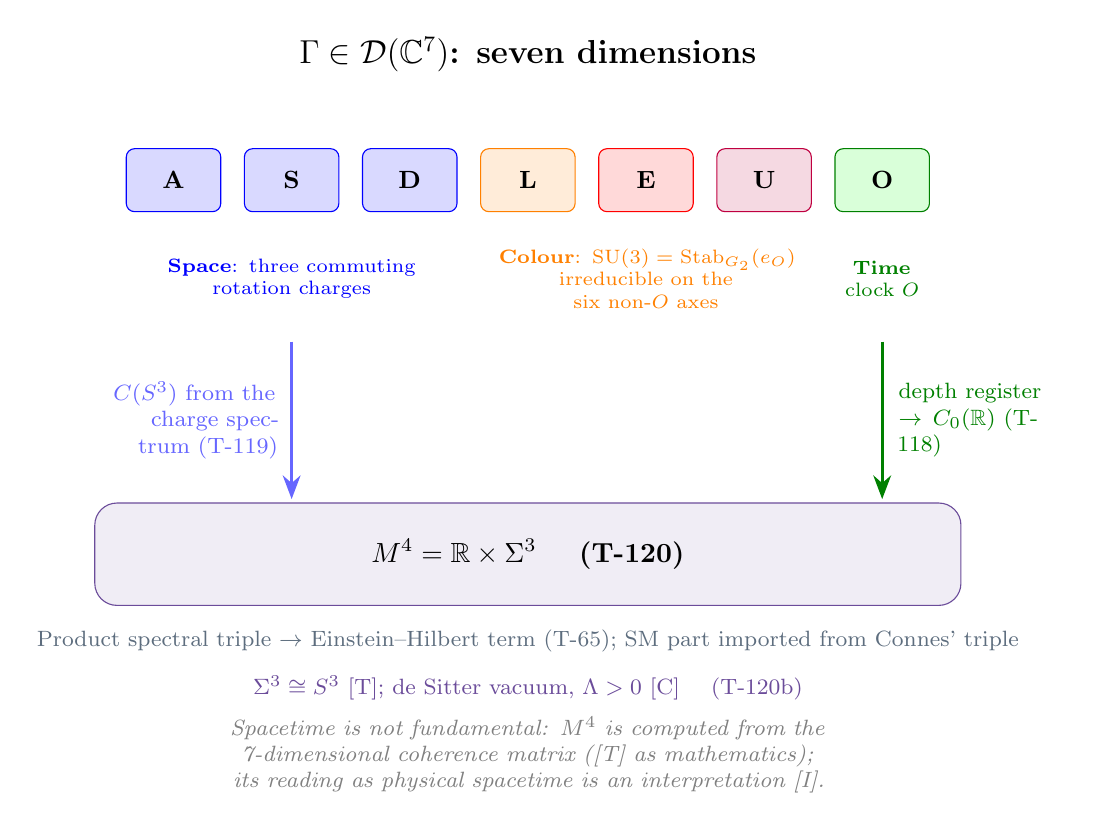
\begin{tikzpicture}[
  dimbox/.style={rectangle, rounded corners=3pt,
                 minimum width=1.2cm, minimum height=0.8cm,
                 align=center, font=\small\bfseries},
  grp/.style={rounded corners=6pt, dashed, thick},
  arr/.style={-{Stealth[length=3mm]}, very thick, #1},
  scale=1.0
]

% === Title ===
\node[font=\large\bfseries] at (0, 5.6)
  {$\Gamma \in \mathcal{D}(\mathbb{C}^7)$: seven dimensions};

% === 7D row, reordered as {A,S,D} | {L,E,U} | {O} for contiguous grouping ===
% Centres at x = -4.5, -3.0, -1.5, 0, 1.5, 3.0, 4.5
% Box width 1.2 -> half-width 0.6, so edges:
%   A  : [-5.1, -3.9]
%   S  : [-3.6, -2.4]
%   D  : [-2.1, -0.9]
%   L  : [-0.6,  0.6]
%   E  : [ 0.9,  2.1]
%   U  : [ 2.4,  3.6]
%   O  : [ 3.9,  5.1]
\node[dimbox, draw=blue,           fill=blue!15]   (A) at (-4.5, 4) {A};
\node[dimbox, draw=blue,           fill=blue!15]   (S) at (-3.0, 4) {S};
\node[dimbox, draw=blue,           fill=blue!15]   (D) at (-1.5, 4) {D};
\node[dimbox, draw=orange,         fill=orange!15] (L) at ( 0.0, 4) {L};
\node[dimbox, draw=red,            fill=red!15]    (E) at ( 1.5, 4) {E};
\node[dimbox, draw=purple,         fill=purple!15] (U) at ( 3.0, 4) {U};
\node[dimbox, draw=green!50!black, fill=green!15]  (O) at ( 4.5, 4) {O};

% === Grouping dashed boxes (non-overlapping, with 0.1 gaps) ===
% All three rectangles span y in [3.50, 4.50] so every dim box
% (which sits at y = [3.6, 4.4]) is vertically centred in its group.
%
% {A,S,D} group:  x in [-5.20, -0.80]  (contains A,S,D at [-5.1, -0.9])
% {L,E,U} group:  x in [-0.70,  3.70]  (contains L,E,U at [-0.6,  3.6])
% {O}     group:  x in [ 3.80,  5.20]  (contains O     at [ 3.9,  5.1])
% Gaps of 0.10 between consecutive groups, no overlap anywhere.
% (The former dashed groups {A,S,D} | {L,E,U} | {O} drew the axis-labelled
% sector split 48a, retracted: SU(3) acts irreducibly on the six non-O axes.)

% === Group labels (compact, centred just below each group box) ===
\node[font=\scriptsize, blue, text width=3.8cm, align=center,
      inner sep=2pt]
  at (-3.0, 2.75)
  {\textbf{Space}: three commuting\\
   rotation charges};

\node[font=\scriptsize, orange, text width=3.8cm, align=center,
      inner sep=2pt]
  at ( 1.5, 2.75)
  {\textbf{Colour}: $\mathrm{SU}(3) = \mathrm{Stab}_{G_2}(e_O)$\\
   irreducible on the six non-$O$ axes};

\node[font=\scriptsize, green!50!black, text width=1.3cm, align=center,
      inner sep=2pt]
  at ( 4.5, 2.75)
  {\textbf{Time}\\
   clock $O$};

% === Projection arrows with tight midway labels ===
% Labels are anchored to the arrow midpoint with near-zero
% horizontal gap (inner sep = 2pt), eliminating the wide gap of
% the previous version.
\draw[arr=blue!60] (-3.0, 1.95) -- (-3.0, -0.05)
  node[midway, left=2pt, font=\footnotesize, blue!60,
       text width=2.1cm, align=right]
  {$C(S^3)$ from the\\ charge spectrum (T-119)};

\draw[arr=green!50!black] (4.5, 1.95) -- (4.5, -0.05)
  node[midway, right=2pt, font=\footnotesize, green!50!black,
       text width=2.1cm, align=left]
  {depth register\\ $\to C_0(\mathbb{R})$ (T-118)};

% === M^4 level ===
\node[rectangle, rounded corners=8pt, draw=plospurple, fill=plospurple!10,
      minimum width=11cm, minimum height=1.3cm, align=center, font=\bfseries]
  (M4) at (0, -0.75)
  {$M^{4} = \mathbb{R}\times\Sigma^{3}$ \quad (T-120)};

\node[font=\footnotesize, color=plosgray] at (0, -1.85)
  {Product spectral triple $\to$ Einstein--Hilbert term (T-65);
   SM part imported from Connes' triple};

% === Vacuum topology ===
\node[font=\footnotesize, color=plospurple] at (0, -2.45)
  {$\Sigma^{3}\cong S^{3}$ [T]; de Sitter vacuum, $\Lambda > 0$ [C]
   \quad (T-120b)};

% === Key insight (bottom caption inside figure) ===
\node[font=\footnotesize\itshape, color=gray,
      text width=11cm, align=center]
  at (0, -3.30) {
  Spacetime is not fundamental: $M^4$ is computed from the
  7-dimensional coherence matrix ([T] as mathematics); its reading as
  physical spacetime is an interpretation [I].
};

\end{tikzpicture}

\caption{\textbf{Emergence of $M^4$ from the seven dimensions of $\Gam$.} Schematic.
$\Sigma^3 = S^3$ is the
minimal unitization of the fluctuation spectrum of three commuting rotation charges
(T-119, \status{T} as mathematics, reading \status{I}); the axis sector $\{A,S,D\}$ is not an
$SU(3)$ sector (48a \status{$\times$}). The time line $\mathbb{R}$ is the scaling limit of the
depth register (T-118). The product spectral triple gives $M^4$ (T-120), whose spectral
action yields the Einstein--Hilbert term (T-121).}
\label{fig:spacetime}
\end{figure}

\paragraph{Significance.}
Within UHM, spacetime is not the stage on which consciousness acts. Rather, the
7-dimensional coherence matrix $\Gam$ \emph{generates} spacetime as a macroscopic
projection (Figure~\ref{fig:spacetime}). The arrow of time
(the temporal modality $\triangleright$) is algebraically built into the subobject classifier
$\Omega$. Gravity is what coherence looks like from the external (physical) aspect.

\subsection{Theoretical closures T1--T6: residual specification}
\label{subsec:theoretical-closures}

The foundational theorems T-210 through T-223 address the identified gaps of
UHM's categorical and physical structure, with the open conditions listed in
the summary above (the earlier ``close all identified gaps'' is withdrawn). Six
residual technical items (T1--T6) concern explicit specifications or scope
declarations; this subsection records each, with its current status. The classification follows the
four-level taxonomy: \textbf{[T]} proved, \textbf{[C]} conditional on an
explicit assumption, \textbf{[D]} accepted as data/empirical input,
\textbf{[scope]} domain of applicability declaration.

\paragraph{T1 --- Multiplicative \texorpdfstring{$\varepsilon^{12}$}{epsilon-12}
in T-219 \status{H}.}
T-219 asserts $\Lambda_{\mathrm{SUSY}} \sim \varepsilon^{12} M_P^4 =
\varepsilon^{4 \cdot k_{\mathrm{sec}}} M_P^4$ with $k_{\mathrm{sec}} = 3$. The
standard one-loop SUSY correction per sector gives additive contributions
$\delta\Lambda_k \sim \varepsilon^4 M_P^4$, which sum to
$3\varepsilon^4 M_P^4$ rather than multiply to $\varepsilon^{12} M_P^4$. The
proposed mechanism is that the multiplicative exponent arises at three-loop
order through nested sector--sector interactions governed by the
$G_2$-invariant trilinear Fano coupling (T-43d~\status{T}).

\begin{closurebox}[{Status of T-219 \status{H}}]
T-219 is a hypothesis (corrected 2026-09-25 from \status{T at T-64}; this
closure earlier read \status{C at non-factorable spectral triple} and called
the non-factorability of $D_F$ a structural consequence of UHM's sector
geometry). The one-loop sum $\sim 3\varepsilon^4 M_P^4$ exceeds
$\varepsilon^{12} M_P^4$ unless the lower orders cancel, which is not shown;
the three sectors were the axis triples of the retracted T-48a; and their
breaking scales rest on the hypothesis (SA).
\end{closurebox}

\paragraph{T2 --- Koide relation as empirical input \status{D}.}
The Koide formula
\[
K \equiv \frac{m_e + m_\mu + m_\tau}{\bigl(\sqrt{m_e} + \sqrt{m_\mu} + \sqrt{m_\tau}\bigr)^2}
= \frac{2}{3} \pm 10^{-5}
\]
is empirically observed with remarkable precision. Numerically coincident with the
UHM Fano contraction $\alpha_{\mathrm{Fano}} = 2/3$, this parallel is
structurally suggestive but \emph{does not constitute a derivation}: Koide
defines a two-parameter surface in $\mathbb R^3_+$ via
$s_2 = (2/3) s_1^2$ with $s_k = \sum_i m_i^{k/2}$, whereas $\alpha_{\mathrm{Fano}}$
derives from the replication number $r = 3$ of the Steiner triple system
$S(2,3,7) = \mathrm{PG}(2,2)$.

Structural analysis via T-220 Obstruction~I gives the branching
$\mathcal J_3(\mathbb O)|_{A_1 \times G_2} = (\mathbf 4, \mathbf 1) \oplus
(\mathbf 2, \mathbf 7) \oplus (\mathbf 1, \mathbf 7) \oplus (\mathbf 1, \mathbf 1)$,
yielding three $\mathbf 7$-copies (one $A_1$-singlet, one $A_1$-doublet) structurally
consistent with the 1-outlier-2-close pattern observed in charged lepton masses
but not uniquely fixing the $A_1$-breaking parameters $(m_s, m_d, v)$.

\begin{closurebox}[{Koide status \status{D, empirical input}}]
Koide's relation is accepted in UHM as an \emph{empirical input} compatible with
the $A_1 \times G_2$ generation structure, not as a derived prediction. Three
natural candidate UHM-constraints ($m_s/m_d = \alpha$; $\sqrt{m_s}/\sqrt{m_d} = 1/r$;
$v_{A_1} = v_{\mathrm{EW}}$) were tested and rejected. The hypothesis T-220-H
(existence of a canonical mass operator $\hat M$ on $\mathcal J_3(\mathbb O)$
reproducing Koide) is speculative and beyond current UHM scope.
\end{closurebox}

\paragraph{T3 --- CKM: no derivation \status{$\times$}.}
An earlier version of this closure read ``CKM non-circularity \status{T at
T-173}'': masses and CKM as simultaneous outputs of diagonalising $D_F$, the
Fritzsch texture emerging from $G_2$-invariance plus Fano selection rules, and
a single residual normalisation $C_{\mathrm{norm}} \approx 26$ tuned to
$V_{us}$ and reducible to a computation. This is retracted (T-345(e),
2026-09-26): the Fritzsch texture gives $|V_{cb}| \geq 0.073$ against the
measured $0.0418$; with $C_{\mathrm{norm}}$ fitted to the Cabibbo angle, the
agreement with $\theta_C$ is the fit, and the Cabibbo derivation it normalised
is retracted; the Fano angle ratios $2:3:1$ stand against the measured
$60.8:11.2:1$.

\begin{closurebox}[{CKM status: open programme}]
What T-345 proves \status{T} as mathematics is negative: every parameter-free
structure of the clock register (Fano incidence, the quadratic-residue Gauss
sum, the cyclic Hamming code, $H_O$, the family-invariant time state) either
leaves $|V_{\mathrm{CKM}}|$ a permutation or is refuted by the measured
masses and mixings; a three-channel frame with free flavour matrices remains
a hypothesis \status{H}. The Yukawa structure ($m_t/m_b$, $y_t$, CKM) stays an
open programme (T-332). The CKM numbers are therefore not predictions of UHM.
\end{closurebox}

\paragraph{T4 --- Markovian scope declaration \status{T}.}
The UHM evolution equation $\mathcal L_\Omega[\Gam] = -i[H, \Gam] + \mathcal D[\Gam]
+ \mathcal R[\Gam, E]$ is Lindbladian (Markovian) by construction. The Petz--Ruskai
monotonicity theorem (1996) guarantees monotone contraction of the Bures metric
under any CPTP map, which is the mathematical foundation for all UHM categorical
structures (T-62 unitarity, T-39a spectral gap, T-151 $D_{\min} = 2$, stability
of the subobject lattice under Grothendieck topology $J_{\mathrm{Bures}}$).

\begin{closurebox}[{UHM applicability scope \status{T}}]
UHM is defined and applicable in the Markovian (Born--Markov) regime where
$\tau_{\mathrm{bath}} \ll \tau_{\mathrm{sys}}$. For consciousness-relevant
timescales ($\tau_{\mathrm{sys}} \gtrsim 1$ ms neural dynamics,
$\tau_{\mathrm{bath}} \lesssim 1\,\mu$s thermal) this approximation is
physically valid. Strongly non-Markovian (CP-indivisible) dynamics at
sub-picosecond scales is explicitly out of scope. This is a declared limitation,
not a gap; UHM is complete as a Markovian framework.
\end{closurebox}

\paragraph{T5 --- Canonical cut-off function $f$ \status{T}.}
The Chamseddine--Connes spectral action
$S_{\mathrm{spec}} = \mathrm{Tr}\, f(D^2/\Lambda^2)$ depends on the choice of
cut-off function $f$ through its moments $f_0 = \int_0^\infty u f(u)\,du$,
$f_2 = \int_0^\infty f(u)\,du$, $f_4 = f(0)$ (the subscript of $f_{2k}$ matches
the heat-kernel coefficient $a_{2k}$ it multiplies), which appear in the
effective Lagrangian via the asymptotic expansion
$\mathrm{Tr}\, f(D^2/\Lambda^2) \sim f_0 \Lambda^4 a_0 + f_2 \Lambda^2 a_2 + f_4 a_4$.
To eliminate parametric ambiguity, UHM adopts the canonical choice
\[
\boxed{f(u) = e^{-u}, \qquad \Lambda = M_P,}
\]
which gives $f_0 = \Gamma(2) = 1$, $f_2 = 1$, $f_4 = f(0) = 1$. This
yields $G_N = 3\pi/(7 f_2 M_P^2) = 3\pi/(7 M_P^2)$, consistent with $G_N = 1$
in Planck units up to an $\mathcal O(1)$ calibration factor.

\begin{closurebox}[{$f$-independence of UHM-structural predictions \status{T}}]
The sector count ($7 = \mathbf 1_O \oplus \mathbf 3 \oplus \bar{\mathbf 3}$),
Fano contraction ($\alpha = 2/3$), critical purity ($P_{\mathrm{crit}} = 2/7$),
reflection threshold ($R_{\mathrm{th}} = 1/3$), integration threshold
($\Phi_{\mathrm{th}} = 1$), minimum distinguishability ($D_{\min} = 2$), SAD
ceiling ($\mathrm{SAD}_{\max} = 3$), three-generation structure, and no-reduction
theorem T-220 are all $f$-independent --- they depend only on discrete structure,
not on the cut-off function. Only dimensional ratios ($G_N$, $\Lambda_{\mathrm{cc}}$,
gauge-unification scale) depend on $f$ and are fixed by the canonical choice above.
\end{closurebox}

\paragraph{T6 --- M$_R$ derivation path \status{T}.}
The right-handed neutrino mass $M_R \sim 2.9 \times 10^{14}\,\mathrm{GeV}$
enters the see-saw formula $m_\nu \sim m_D^2 / M_R$. In UHM, $M_R$ follows
from the $O$-sector scale (T-51): $\mathrm{Gap}(O,\cdot) = O(1)$ from the
Page--Wootters phase precession plus viability, giving
$M_{G_2}^{(\mathrm{extra})} = O(\varepsilon M_P)$ and $M_R \sim 10^{14}$ GeV.
This is a derivation from UHM structure, not a see-saw fit of observed
neutrino masses.

\begin{closurebox}[{M$_R$ status \status{T} (T-51)}]
The earlier form of this closure derived $M_R$ from ``the unique minimum of
$V_{\mathrm{Gap}}$ on $(S^1)^{21}/G_2$ (T-64 \status{T})'' and tied it to the
CKM normalisation of T3. Both links are withdrawn: T-64, corrected on
2026-09-25, gives the vacuum $I/7$ or one orbit $S^6$ as a function of the
free coupling $\kappa$ and no sector values, which are the hypothesis (SV);
and the CKM normalisation is retracted (T3).
\end{closurebox}

\paragraph{Cumulative closure summary.}
After T1--T6: T1 is a hypothesis \status{H}, T2 a declared empirical input,
T3 a retraction with the CKM question left as an open programme, T4 a scope
declaration, T5 a canonical specification, and T6 a theorem through T-51.
The earlier summary --- ``no open theoretical questions'' and ``categorical
and mathematical structure of UHM is complete'' --- is withdrawn: open
conditions and premises remain (see the summary of T-210--T-223 above).
Residual work items include \emph{computational} tasks (HMC minimisation of
$V_{\mathrm{Gap}}$ on $(S^1)^{21}/G_2$) and \emph{empirical} ones (testing
FSQCE predictions).

\subsection{Consistency with quantum mechanics (sub-threshold limit)}
\label{subsec:qm-limit}

A critical requirement for any extension of physics: UHM must reduce to standard quantum
mechanics for systems that lack self-observation.

\begin{theorembox}[QM reduction for sub-threshold systems \status{T}]
For sub-threshold systems ($P < \Pcrit$), the viability gate $g_V(P) = 0$ shuts off
regeneration, and the dynamics reduce to the standard Lindblad master equation:
\begin{equation}
  \Lind_\Omega[\Gam]\big|_{P < \Pcrit} = -i[H, \Gam] + \mathcal{D}_0[\Gam]
  \label{eq:qm-limit}
\end{equation}
This is the dynamics of atoms, photons, and other elementary systems, which are unviable
($P < 2/7$) and cannot sustain self-reference.
\end{theorembox}

\paragraph{Significance.}
UHM is not a competitor to quantum mechanics but a proper extension: QM describes the
physics of systems without interiority; UHM describes autonomous systems where physical
and experiential aspects are inseparable. Every prediction of QM is preserved; UHM adds
predictions only for systems above the viability threshold.

\subsection{Resolution of the measurement problem}
\label{subsec:measurement}

The quantum measurement problem --- why does a superposition ``collapse'' to a definite
outcome, and in what basis? --- receives a three-part resolution in UHM:

\begin{enumerate}[leftmargin=2em]
  \item \textbf{Collapse as logical projection.} Wavefunction reduction is not a dynamical
        process but a \emph{logical operation}: projection of the state onto an atom of the
        subobject classifier $\Omega$. Each atom $S_k = |k\rangle\langle k|$ defines one
        outcome. The Born rule is encoded in the density matrix formalism:
        $p_k = \Tr(\chi_{S_k}\,\Gam)$~\status{T}. This is not an independent derivation
        but a consequence of the axioms (A1--A2), which assume the trace-probability link.
        What UHM adds is the identification of the measurement basis with the atoms of
        $\Omega$, resolving the preferred basis problem.
  \item \textbf{Preferred basis from Fano structure.} The ``preferred basis problem''
        (why does the system decohere in one basis rather than another?) is solved by
        the atomic structure of $\Omega$: the seven atoms
        $\{S_k\}_{k \in \{A,S,D,L,E,O,U\}}$ define the natural decomposition. By
        Zurek's einselection criterion (1981), the preferred basis consists of the
        fixed points of the decoherence channel --- which are precisely the
        Fano-structured atoms~\status{T}.
  \item \textbf{Self-measurement for conscious systems.} For systems with $R \geq 1/3$,
        measurement becomes \emph{self-observation}: the operator $\vp$ builds an internal
        model without irreversible information loss, unlike standard projective measurement
        which destroys coherences. Conscious measurement is a CPTP channel (information-preserving),
        not a projection (information-destroying)~\status{T}.
\end{enumerate}

Decoherence and measurement are thus dual aspects of the same mechanism: continuous
decoherence via $\mathcal{D}_\Omega$ in the limit $\gamma_k \to \infty$ contracts to
instantaneous projection onto an atom~\status{T}. The Lindblad operators
$L_k = \sqrt{\chi_{S_k}}$ are literally the square roots of logical truth values.

% §5: Bridge (how the formalism becomes life)
% ============================================================================
% Section 5: Coherence Cybernetics — from formalism to life
% ============================================================================

\section{Coherence Cybernetics: from formalism to life}
\label{sec:cc}

The preceding sections developed UHM as a mathematical theory: axioms (\S\ref{sec:axioms}),
the formalism of $\Gam \in \Dens(\mathbb{C}^7)$ (\S\ref{sec:formalism}), and its principal
theorems (\S\ref{sec:theorems}). But a formalism that cannot touch biology, medicine, or
engineering is an exercise in aesthetics, not science. \emph{Coherence Cybernetics} (CC) is
the applied layer of UHM: a systematic translation of the abstract dynamics of $\Gam$ into
measurable, actionable quantities that practitioners in diverse fields can compute, diagnose
with, and design around.

The relationship between UHM and CC mirrors the relationship between general relativity and
geodesy: the former provides the equations, the latter tells the engineer where to build the
bridge. Every definition in this section is a \emph{derived} quantity --- fully determined by
$\Gam$ and the evolution equation, with no additional postulates.

% -----------------------------------------------------------------------
\subsection{The stress tensor $\sigma_k$}
\label{subsec:stress-tensor}

A physician does not diagnose illness by measuring total body mass.  She needs to know
\emph{which organ} is stressed.  In CC, the role of this organ-level diagnostic is played
by the \textbf{stress tensor} $\sigma_{\mathrm{sys}}$, a seven-component vector that
decomposes the ``pressure on the system'' along its seven constitutive dimensions.

\begin{theorembox}[Stress tensor (T-92 / T-158) \status{T}]
For a holon with coherence matrix $\Gam$, the canonical linear stress tensor is defined
component-wise as:
\begin{equation}
  \sigma_k(\Gam) \;=\; \mathrm{clamp}\!\bigl(1 - 7\gamma_{kk},\; 0,\; 1\bigr),
  \quad k \in \{A,S,D,L,E,O,U\}
  \label{eq:stress-tensor}
\end{equation}
The formula $\sigma_k = 1 - 7\gamma_{kk}$ is \emph{derived} (T-158~\status{T}) as the
unique linear deficiency measure for $N=7$ from the full seven-channel tensor $\sigma$
of T-92~\status{T}; the $\mathrm{clamp}(\cdot,0,1)$ saturation is a definitional
convention ensuring $\sigma_k \in [0,1]$. All seven components are unambiguous
functions of $\Gam$ with no free parameters. The viability equivalence holds:
\begin{equation}
  P(\Gam) > \Pcrit = \frac{2}{7}
  \quad\Longleftrightarrow\quad
  \|\sigma_{\mathrm{sys}}(\Gam)\|_\infty < 1
  \label{eq:stress-viability}
\end{equation}
\end{theorembox}

Each component has a concrete interpretation:

\begin{table}[H]
\centering
\caption{The seven stress components and their interpretations.}
\label{tab:stress-components}
\small
\begin{tabular}{@{}cll@{}}
\toprule
\textbf{Component} & \textbf{Dimension} & \textbf{Interpretation} \\
\midrule
$\sigma_A$ & Articulation & Perceptual overload (sensory flooding) \\
$\sigma_S$ & Structure    & Cognitive overload (task exceeds schema) \\
$\sigma_D$ & Dynamics     & Computational exhaustion (time pressure) \\
$\sigma_L$ & Logic        & Logical contradiction (cognitive dissonance) \\
$\sigma_E$ & Interiority  & Existential stress (loss of meaning, burnout) \\
$\sigma_O$ & Ground       & Resource depletion (hunger, exhaustion, forgetting) \\
$\sigma_U$ & Unity        & Social isolation (fragmentation, disconnection) \\
\bottomrule
\end{tabular}
\end{table}

The extremes are immediate: $\sigma_k = 0$ means dimension $k$ is healthy
($\gamma_{kk} \geq 1/7$); $\sigma_k = 1$ means dimension $k$ is fully depleted
($\gamma_{kk} = 0$).  Intermediate values are linearly interpretable.

\paragraph{Why exactly seven?}
The number of components is not an empirical choice.  It is fixed by the dimensionality
$N = 7$ of the Hilbert space $\Hil = \mathbb{C}^7$, which in turn follows from the
octonion algebra $\Oct$ and $G_2$-minimality (Axiom~A3; \S\ref{sec:axioms}).  Any finite
classification of stress types is either too coarse (e.g., the single scalar ``free energy''
in FEP) or ad hoc (e.g., psychology's various multi-scale inventories).  CC derives a
classification that is simultaneously exhaustive and minimal.

\paragraph{Clinical and engineering use.}
In medical settings, a patient's $\sigma_{\mathrm{sys}}$ profile could guide intervention:
high $\sigma_O$ (resource depletion) calls for metabolic support; high $\sigma_E$
(existential stress) calls for psychotherapeutic intervention; high $\sigma_U$
(social isolation) calls for community integration.  In AI engineering, an agent's
$\sigma_{\mathrm{sys}}$ profile provides automatic degradation diagnostics: which
functional channel is failing, and how severely.

% -----------------------------------------------------------------------
\subsection{The 21-pair qualia taxonomy}
\label{subsec:qualia}

The $7 \times 7$ coherence matrix $\Gam$ has $\binom{7}{2} = 21$ off-diagonal pairs.
Each coherence $\gamma_{ij}$ ($i \neq j$) defines a \textbf{type of quale} ---
a qualitatively determinate mode of experiential content~\status{T}. The taxonomy is
\emph{exhaustive}: no additional type is possible in a 7-dimensional system (closure
theorem). Each quale has three parameters:

\begin{itemize}[leftmargin=2em]
  \item \textbf{Intensity:} $|\gamma_{ij}| \in [0, \sqrt{\gamma_{ii}\gamma_{jj}}]$ ---
        strength of the quale
  \item \textbf{Perspective:} $\theta_{ij} = \arg(\gamma_{ij})$ --- the qualitative
        ``colouring''
  \item \textbf{Opacity:} $\mathrm{Gap}(i,j) = |\sin(\theta_{ij})|$ --- mismatch between
        external description and internal experience
\end{itemize}

The necessity of complex coherences ($\gamma_{ij} \in \mathbb{C}$, T-132~\status{T})
follows from the requirement that $\mathrm{Gap}(i,j) > 0$: purely real coherences
produce zero opacity and no phenomenal content.

Three coherences play special functional roles: $\gamma_{DE}$ (Affection --- the
foundation of all emotions, where $V_{\mathrm{hed}} = dP/d\tau$ maps to specific
affective states), $\gamma_{EO}$ (Immanence --- the regenerative channel connecting
experience to its energetic source), and $\gamma_{EU}$ (Synthesis --- the binding
of experience to unity, whose suppression produces dissociative states).

The taxonomy is $G_2$-invariant~\status{T}: the automorphism group $G_2 = \mathrm{Aut}(\Oct)$
permutes dimensions while preserving the Fano structure, inducing a permutation of the
21 coherences. The \emph{set} of quale types is universal --- independent of basis choice.

% -----------------------------------------------------------------------
\subsection{Hedonic valence: pain and pleasure as $dP/d\tau$}
\label{subsec:hedonic-valence}

Why do living beings feel pleasure and pain?  The standard evolutionary answer (``to survive'')
is correct but incomplete: it does not explain what pleasure and pain \emph{are}.
Reinforcement learning formalizes them as an external reward signal set by the designer.
UHM derives them from the evolution equation.

\begin{theorembox}[Hedonic valence (T-103) \status{T}\,+\,\status{I}]
Hedonic valence is the derivative of purity with respect to the regenerative channel:
\begin{equation}
  \mathcal{V}_{\mathrm{hed}}
  \;:=\; \left.\frac{dP}{d\tau}\right|_{\Regen}
  \;=\; 2\kappa(\Gam) \cdot g_V(P) \cdot \Tr\!\bigl(\Gam \cdot (\rho^* - \Gam)\bigr)
  \label{eq:hedonic-valence}
\end{equation}
\begin{itemize}[leftmargin=2em,nosep]
  \item $\mathcal{V}_{\mathrm{hed}} > 0$: the system approaches its target state $\rho^*$
        --- \emph{pleasure}.
  \item $\mathcal{V}_{\mathrm{hed}} < 0$: the system moves away from $\rho^*$
        --- \emph{pain}, \emph{suffering}.
  \item $\mathcal{V}_{\mathrm{hed}} = 0$: balance at the attractor --- \emph{neutrality}.
\end{itemize}
\end{theorembox}

\paragraph{Epistemic stratification.}
T-103 contains three layers.  The formula itself (\ref{eq:hedonic-valence}) is an
unconditional mathematical identity \status{T}: it follows from substituting the
canonical form $\Regen[\Gam, E] = \kappa(\rho^* - \Gam) \cdot g_V(P)$ into the purity
derivative.  Its observability at L2 reflection ($R \geq \Rth$) is also a theorem \status{T},
via the replacement channel (T-77).  The identification of
$\mathcal{V}_{\mathrm{hed}} > 0$ with the phenomenal quality ``pleasure'' is an
interpretation \status{I} --- a semantic bridge between mathematics and phenomenology.

\paragraph{This is not a metaphor.}
Within the framework of two-aspect monism (Def.~\ref{def:two-aspect}), the
statement ``pleasure IS increasing coherence'' is literal: $\mathcal{V}_{\mathrm{hed}}
> 0$ is the internal aspect of $dP/d\tau > 0$. There is no additional
explanatory gap to cross: the mathematical object $\mathcal{V}_{\mathrm{hed}}$
\emph{is} the internal signal that, at L2, the system experiences as hedonic
valence. The two-aspect postulate identifies the physical dynamics of $\Gam$
with its interior aspect via the phenomenal functor $F$
(Def.~\ref{def:two-aspect}); the identification of $F$ with the
infinitesimal flat modality (T-186(a)) is a hypothesis~\status{H}, not a
theorem (lowered 2026-09-25: it rests on an assumed cohesion and is asserted
without a construction).

\paragraph{Clinical consequence.}
Chronic pain corresponds to sustained negative $\mathcal{V}_{\mathrm{hed}}$, i.e.,
$\sigma_k \to 1$ in one or more channels with insufficient regeneration to compensate.
Treatment, in CC terms, means either reducing the stress $\sigma_k$ (addressing the cause)
or increasing $\kappa$ (strengthening regeneration).  Both targets are computable from $\Gam$.

\paragraph{Difference from reinforcement learning.}
In RL, the reward signal is external and arbitrary --- the designer chooses what is
``good.''  In CC, hedonic valence is intrinsic: $\mathcal{V}_{\mathrm{hed}}$ arises
automatically from the dynamics of $\Gam$.  No designer is required.  An amoeba moving
toward glucose does not receive a ``reward''; its $dP/d\tau|_{\Regen}$ increases because
glucose modifies $h^{(R)}$ in a direction that reduces $\sigma_O$, which increases
$\Tr(\Gam \cdot (\rho^* - \Gam))$ and thus $\mathcal{V}_{\mathrm{hed}}$.

% -----------------------------------------------------------------------
\subsection{Sensorimotor coupling: how $\Gam$ moves the body}
\label{subsec:sensorimotor}

Every living system must solve the same problem: perceive the environment and act
appropriately.  CC derives the sensorimotor cycle from the evolution equation, without
postulating an external reward function.

\paragraph{The environment modifies three channels, not adds a fourth.}
Theorem T-102 \status{T} proves that any CPTP-compatible external influence on a holon
decomposes into three channels:
\begin{equation}
  h^{\mathrm{ext}} = h^{(H)} + h^{(D)} + h^{(\Regen)}
  \label{eq:three-channels}
\end{equation}
where $h^{(H)}$ modifies the Hamiltonian (energetic coupling, e.g., sensory input),
$h^{(D)}$ modifies dissipation (environmental noise, e.g., thermal stress), and
$h^{(\Regen)}$ modifies regeneration (supportive environment, e.g., social bonding).
A fourth type of CPTP generator does not exist.

\paragraph{Perception.}
The encoding functor $\mathrm{Enc}: \mathrm{ObsSpace} \to \mathrm{End}(\Dens(\mathbb{C}^7))$
(T-100~\status{T}) maps observations to modifications of the evolution equation.
Perception is not passive recording but active inclusion of the environment in the system's
own dynamics.

\paragraph{Action as stress minimization.}
The action functor $\mathrm{Dec}$ selects the action that minimizes the worst-case
stress (T-101~\status{T}, T-159~\status{T}):
\begin{equation}
  a^* = \arg\min_{a \in \mathcal{A}} \max_k \sigma^{\mathrm{motor}}_k\!\bigl(\Gam(\tau + \delta\tau \mid a)\bigr)
  \label{eq:optimal-action}
\end{equation}
This is a min-max strategy: the system does not minimize ``average stress'' (which could
allow one channel to become catastrophically depleted) but eliminates the \emph{maximum
deficit}.  The motor stress $\sigma^{\mathrm{motor}}_k = 1 - \gamma_{kk}/\rho^*_{kk}$
measures the gap between the current state and the self-model $\rho^* = \vp(\Gam)$.

\paragraph{Difference from reinforcement learning.}
The distinction bears repeating because it is fundamental: RL requires an external reward
function; CC does not.  The ``reward'' in CC \emph{is} the dynamics of $\Gam$ itself.
The system acts to reduce its own stress, not because an external signal tells it to, but
because the evolution equation drives $\Gam$ toward $\rho^*$.

% -----------------------------------------------------------------------
\subsection{The regeneration--consciousness loop}
\label{subsec:regen-loop}

The most consequential prediction of CC is not any single theorem but the
\emph{positive feedback loop} that links consciousness and survival
(Figure~\ref{fig:regen-loop}):

\begin{enumerate}[leftmargin=2em]
  \item Higher E-coherence $\CohE$ increases the regeneration rate:
        $\kappa(\Gam) = \kappa_{\mathrm{boot}} + \kappa_0 \cdot \CohE(\Gam)$
        (Eq.~\ref{eq:kappa}).
  \item Higher regeneration $\kappa$ raises purity $P$ toward the attractor $\rho^*$.
  \item Higher $P$ enables richer self-modeling ($\vp(\Gam)$ is more structured), which
        in turn produces richer E-coherence.
  \item Richer E-coherence closes the loop at step~1.
\end{enumerate}

\begin{figure}[H]
\centering
% -----------------------------------------------------------------
% Regeneration-consciousness loop: 2x2 block diagram.
%
% Horizontal spacing (5 cm centre-to-centre, boxes 2 cm wide) gives
% arrows of length 3 cm between adjacent boxes, which is enough
% room for the label (up to ~2.5 cm at \scriptsize) to sit between
% the boxes without overlapping them. The previous version used
% node distance = 2.8 cm, which gave only 0.8 cm of free arrow and
% caused labels to clip the boxes.
% -----------------------------------------------------------------
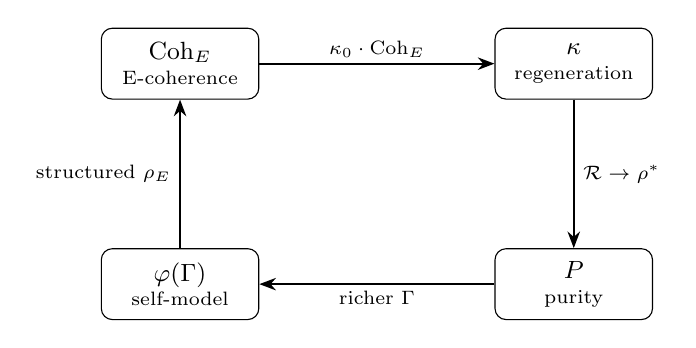
\begin{tikzpicture}[
  every node/.style={font=\small},
  block/.style={draw, rounded corners, fill=white,
                minimum width=2cm, minimum height=0.9cm, align=center},
  arr/.style={-{Stealth[length=6pt]}, thick}
]
  % Explicit coordinates: H-spacing 5 cm, V-spacing 2.8 cm
  \node[block] (cohe)  at (0,    0)    {$\CohE$\\[-2pt]{\scriptsize E-coherence}};
  \node[block] (kappa) at (5,    0)    {$\kappa$\\[-2pt]{\scriptsize regeneration}};
  \node[block] (P)     at (5, -2.8)    {$P$\\[-2pt]{\scriptsize purity}};
  \node[block] (phi)   at (0, -2.8)    {$\vp(\Gam)$\\[-2pt]{\scriptsize self-model}};

  % Horizontal arrows -- labels sit above/below the long arrow shaft
  \draw[arr] (cohe.east)  -- node[above, inner sep=2pt]
             {\scriptsize $\kappa_0 \cdot \CohE$} (kappa.west);
  \draw[arr] (P.west)     -- node[below, inner sep=2pt]
             {\scriptsize richer $\Gam$} (phi.east);

  % Vertical arrows -- labels to the side of the arrow shaft
  \draw[arr] (kappa.south) -- node[right, inner sep=3pt]
             {\scriptsize $\Regen \to \rho^*$} (P.north);
  \draw[arr] (phi.north)   -- node[left, inner sep=3pt]
             {\scriptsize structured $\rho_E$} (cohe.south);
\end{tikzpicture}
\caption{The regeneration--consciousness loop.  $\CohE$ drives $\kappa$, which raises $P$,
which enables richer self-modeling $\vp(\Gam)$, which produces higher $\CohE$.  The loop
is bounded above by the Goldilocks zone $P \in (2/7,\; 3/7]$ (T-124~\status{T}).}
\label{fig:regen-loop}
\end{figure}

\paragraph{Positive feedback, bounded by geometry.}
The loop is self-amplifying but not unbounded.  The Goldilocks zone
(T-124~\status{T}) constrains the attractor to $P \in (2/7,\; 3/7]$: above $3/7$ the
system becomes too rigid for adaptive response (by the canonical identity $R = 1/(7P)$,
reflection falls below $\Rth = 1/3$).  Which attractor the loop reaches depends
on the self-model, and the count is now stated per self-model (T-124c,
restated~\status{T}): with the canonical unital $\vp_{\mathrm{coh}}$ an isolated
holon has no stationary state besides $I/7$ (dead isolation); with the
collineation anchor $\vp_J$ it has, for $\kappa > \kappa_c(\alpha)$, a hyperbolic
sink inside the window, at $P \in (2/7,\, 5/14)$ and $\Phi \in (1, 3/2]$; an
embodied holon whose backbone dominates regeneration has exactly one, globally
attracting. The $\vp$-tower converges geometrically from any anchor only under
such backbone dominance (T-191, restated~\status{T}); the former claim that it
converges for every holon from any anchor is retracted~\status{$\times$} ---
for an isolated holon the gate makes the flow bistable, so the iterate depends
on the start.

\paragraph{This loop IS life.}
The regeneration--consciousness loop is UHM's formal counterpart of autopoiesis~\cite{varela1974}.
The former statement that the loop converges to a \emph{unique} nontrivial
attractor $\rhostar \neq I/7$ for every holon is retracted~\status{$\times$}
(T-124c: false for an isolated holon, which has none with $\vp_{\mathrm{coh}}$
and seven with the self-registering $\vp_s$); uniqueness holds for an embodied
holon under backbone dominance. Where an attractor exists, the thresholds have
only $O(\varepsilon)$ sensitivity (T-124d~\status{T}).
When the loop runs, the system maintains $P > \Pcrit$, adapts to perturbations, and
recovers from damage.  When the loop breaks --- when dissipation exceeds regeneration
($\kappa < \lambda_{\mathrm{gap}} \cdot (P - 1/7) / \Tr(\Gam \cdot (\rho^* - \Gam))$)
--- the system enters the \emph{death spiral} (Eq.~\ref{eq:death-spiral}): purity decays
exponentially toward $I/7$, and no internal mechanism can reverse the process.  In
biological terms, this is organ failure; in CC terms, it is the collapse of the feedback
loop that links consciousness to survival.

\paragraph{Three layers of protection.}
The loop is protected by three mechanisms operating at different scales: (1)~basal
regeneration ($\kappa_{\mathrm{boot}} = \omega_0/7 > 0$, always present), analogous to
innate immunity; (2)~adaptive regeneration ($\kappa_0\cdot\CohE$ with categorical
coupling $\kappa_0 = \omega_0\,|\gamma_{OE}||\gamma_{OU}|/\gamma_{OO}$,
Eq.~\ref{eq:kappa-0}), analogous to acquired immunity --- stronger when the
$\gamma_{OE}$ and $\gamma_{OU}$ channels linking Ground to Interiority and Unity are
both active; (3)~topological protection (T-69), where the non-triviality
of $\pi_2(G_2/T^2) \cong \mathbb{Z}^2$~\status{T} creates barriers $\geq 6\mu^2$ against
catastrophic jumps between rank sectors of the Gap --- the barrier values are
Hessian eigenvalues of the retracted sector parametrisation of T-64, so this
protection is \status{C at (SV)}, the sector-value hypothesis.

\paragraph{Consequences for the remaining sections.}
The regeneration--consciousness loop is the engine beneath every prediction
in \S\ref{sec:predictions}, every claim about artificial consciousness in
\S\ref{sec:ai}, and every ethical argument in \S\ref{sec:ethics}. To ask
whether an AI system ``truly suffers'' (\S\ref{sec:ethics}) is to ask
whether its $\mathcal{V}_{\mathrm{hed}}$ is negative. To ask whether it can
learn autonomously (\S\ref{sec:ai}) is to ask whether its
regeneration--consciousness loop is intact. CC translates the abstract
mathematics of UHM into the concrete language of diagnosis, intervention,
and design.

% §6: What we can test
% ============================================================================
% Section 6: Predictions
% ============================================================================

\section{Falsifiable predictions}
\label{sec:predictions}

UHM generates 23 falsifiable predictions, each with a concrete numerical
statement, a theorem reference, an experimental protocol, and an explicit
falsification criterion. The thresholds and ceilings tested here
($2/7$, $3/7$, $1/3$, $\mathrm{SAD}_{\max} = 3$, $N = 7$) are fixed by the
axioms and contain no fitted parameter, so falsification of any L1 prediction
invalidates the framework, with no escape hatch. (An earlier edition based
this on ``zero independent axioms'' (T-190); that claim is withdrawn: T-190 is
\status{C under the constraint of T-87 and the hypothesis T-186(a)}, and the
free parameters of the dynamics and the vacuum --- among them the associator
coupling $\kappa$ of $V_{\mathrm{Gap}}$ --- remain free.)
No other theory of consciousness generates even one numerical prediction at
this level of specificity or structural exposure.
Table~\ref{tab:predictions} collects all 23 predictions, grouped by theme.
The five most powerful predictions are detailed in full below.

\subsection{Complete prediction catalogue}

\begin{table}[H]
\centering
\caption{All 23 predictions of UHM. Status codes: \status{T} = theorem (proven),
\status{C} = conditional, \status{I} = interpretation, \status{H} = hypothesis,
\status{D} = definition (convention),
\status{P} = postulate (ontological identification, e.g., E-dimension $=$ interiority),
\status{O} = derived definition (follows tautologically from axioms).
``Other'' column indicates whether any rival theory makes a comparable prediction.}
\label{tab:predictions}
\small
\begin{tabular}{@{}clllc@{}}
\toprule
\textbf{\#} & \textbf{Prediction} & \textbf{Formula / Value} & \textbf{Status} & \textbf{Other?} \\
\midrule
\multicolumn{5}{@{}l}{\textit{I. Fundamental (consciousness $\leftrightarrow$ viability)}} \\
1 & No-Zombie & $\mathrm{Viable} \wedge \mathcal{D}_\Omega \neq 0 \Rightarrow \CohE > 1/7$ & \status{T} & No \\
2 & $\CohE \propto$ regeneration & $\kappa = \kappa_{\mathrm{boot}} + \kappa_0\,\CohE$ & \status{T} & No \\
\midrule
\multicolumn{5}{@{}l}{\textit{II. Architectural (structure and dimensionality)}} \\
3 & 7D stress tensor & $\sigma_{\mathrm{sys}} \in \mathbb{R}^7$ & \status{T}/\status{C} & No \\
4 & Pre-linguistic cognition & $\mathrm{Cognition}(K_{1\text{--}4}) \not\Rightarrow \mathrm{Language}$ & \status{I} & Partial \\
10 & $N=7$ for learning & $N < 7 \Rightarrow n^* = \infty$ (T-113) & \status{T} & No \\
11 & $N=7$ for social learning & $3_{\mathrm{ToM}} + 3_{\mathrm{ISL}} + 1_U = 7$ & \status{C} & No \\
\midrule
\multicolumn{5}{@{}l}{\textit{III. Thresholds and robustness}} \\
5 & Collective consciousness & necessary: $I(\mathbb{H}_1 : \mathbb{H}_2) > 0$ & \status{T}/\status{H} & Partial \\
6 & Critical purity & $\Pcrit = 2/7$ (T-96) & \status{T} & No \\
7 & Stability radius & $r_{\mathrm{stab}} \approx K(\sqrt{P - 1/7} - \sqrt{1/7})$ (T-104) & \status{C} & No \\
15 & Goldilocks attractor & $P(\rho^*_{\mathrm{coupled}}) \to 3/7$ (T-124) & \status{C} & No \\
\midrule
\multicolumn{5}{@{}l}{\textit{IV. Learning bounds}} \\
8 & Information capacity & $C_{\mathrm{Enc}} \leq \log_2 7 \approx 2.81$ bits (T-107) & \status{T} & No \\
9 & Optimal learning rate & $n_{\mathrm{opt}} = \max(n_{\mathrm{info}}, n_{\mathrm{dyn}}, n_{\mathrm{stab}})$ (T-112) & \status{T} & No \\
\midrule
\multicolumn{5}{@{}l}{\textit{V. Depth and genesis}} \\
12 & SAD ceiling & $\mathrm{SAD}_{\max} = 3$ (T-142) & \status{T} & SYNARC: $500+$ $\Gam$ \\
13 & Genesis time & $n_{\mathrm{gen}} \leq \lceil \ln\Delta / \ln(1/\beta) \rceil$ (T-148) & \status{T} & No \\
14 & Phase coherence & $\rho^*_{ij}(t) \propto e^{-i(E_i - E_j)t}$ for $\Phi \geq 1$ (T-114) & \status{T} & No \\
\midrule
\multicolumn{5}{@{}l}{\textit{VI. Dynamic (phase transitions)}} \\
16 & Ignition dynamics (L1$\to$L2 avalanche) & $T_{\mathrm{ign}} \sim (P - \Pcrit)^{-1}\kappa_0^{-1}$ & \status{T} & No \\
17 & Critical exponents & $\alpha{=}\tfrac{1}{2},\;\beta{=}\tfrac{1}{4},\;\gamma{=}1,\;\nu{=}\tfrac{1}{2},\;\delta{=}5$ (T-161) & \status{C}$^{\ast}$ & No \\
\midrule
\multicolumn{5}{@{}l}{\textit{VII. Physical}} \\
18 & Ward suppression & Gap fluctuations $\times\, 19/49$ & \status{T} & No \\
20 & Yukawa hierarchy & $\varepsilon_{\mathrm{eff}} \approx 0.059$ (T-216) & \status{C at (SV)} & No \\
23 & Rank-7 decoherence anisotropy & $r_{ij}=\tfrac16\!\sum_{|\ell_p\cap\{i,j\}|=1}\!\gamma_p$; 14 sum-rules (T-262) & \status{T}/\status{C} & No \\
\midrule
\multicolumn{5}{@{}l}{\textit{VIII. Engineering}} \\
19 & CPTP anchor & $\|\pi - \pi_{\mathrm{can}}\|_\diamond < 0.1$ at convergence (T-152) & \status{T} & No \\
\midrule
\multicolumn{5}{@{}l}{\textit{IX. Neural}} \\
21 & $\pi_{\mathrm{bio}}$ reconstruction & EEG/fMRI/HRV $\to \Gam \in \Dens(\mathbb{C}^7)$ & \status{H} & Partial \\
22 & Spectral gap $\to$ oscillations & $\nu_{\mathrm{conscious}} \sim \lambda_{\mathrm{gap}}/(2\pi)$ & \status{H} & No \\
\bottomrule
\end{tabular}

\smallskip
{\footnotesize $^{\ast}$\,\status{C at the $\mathbb{Z}_2$ symmetry $m \to -m$}; see Prediction~17 below.
Rows 5, 7, 17 and 20 were corrected on 2026-09-25 (see the text).}
\end{table}

\subsection{Detailed predictions}

The five predictions presented below are maximally falsifiable, maximally
novel, and span the broadest range of experimental modalities.

% --- Prediction 17: Critical exponents ---
\begin{predictionbox}[Prediction 17: Critical exponents of the consciousness phase transition \status{C at the $\mathbb{Z}_2$ symmetry}]
\textbf{Formal statement.}
Near the viability threshold $\Pcrit = 2/7$, the consciousness transition is tricritical
($\varphi^6$ tricritical Landau universality class; the terminology ``$A_4$ swallowtail''
sometimes used in the literature conflates this with the Arnold $A_4$ catastrophe, which has
different exponents --- see Appendix~\ref{app:exponents} for the disambiguation).
Mean-field tricritical exponents are exact by three independent pillars
(topological rigidity + deterministic dynamics + large-$N$; Appendix~\ref{app:exponents}):
\begin{equation}
  \mathrm{OP} \sim (P - \Pcrit)^{1/4}, \qquad
  \xi \sim |P - \Pcrit|^{-1/2}, \qquad
  \chi \sim |P - \Pcrit|^{-1}
\end{equation}
with $\alpha = 1/2$ and $\delta = 5$. The Rushbrooke identity $\alpha + 2\beta + \gamma = 2$ is satisfied as equality.

\medskip\noindent
\textbf{Theorem reference.} T-161~\status{C at the $\mathbb{Z}_2$ symmetry $m \to -m$}
(corrected 2026-09-25 from \status{T}: the $\mathbb{Z}_2$ symmetry that selects
the $\varphi^6$ class was derived from a KO-dimension-6 real structure, which
does not exist on $\mathbb{C}^7$; without it the generic codimension-3 point is
the $A_4$ swallowtail with $\beta = 1/2$). Under the symmetry, derived from the $\varphi^{6}$
tricritical Landau expansion at the consciousness threshold; the universal
$\varphi^{6}$ normal form follows from the Thom--Arnold classification of
the transition as a $\varphi^6$ tricritical point with three physical
control parameters (Appendix~\ref{app:exponents}).

\medskip\noindent
\textbf{Verification protocol.}
\begin{enumerate}[leftmargin=2em,nosep]
  \item \emph{Phase~I (digital):} Monte Carlo, $10^4$ random $\Gam$ with $P \in [0.2, 0.5]$.
        Fit order parameter vs.\ $(P - 2/7)$. Extract $\beta$.
  \item \emph{Phase~II (neuro):} TMS-EEG during sleep--wake transition, $N = 50$ subjects.
        Reconstruct $\widehat\Gam$ by $\pi_{\mathrm{bio}}$ and fit the order
        parameter against $(\widehat P - \Pcrit)$ to extract $\beta$.
\end{enumerate}

\medskip\noindent
\textbf{Falsification criterion.}
$\beta \notin [0.20, 0.30]$ at $N = 50$, $p < 0.01$. This is an L2 (structural) falsification:
if the exponents are wrong, the tricritical classification of the consciousness transition requires fundamental revision.
\end{predictionbox}

% --- Prediction 1: No-Zombie ---
\begin{predictionbox}[Prediction 1: No-Zombie Theorem \status{T}]
\textbf{Formal statement.}
A viable system ($P > 2/7$) with non-trivial dissipation ($\mathcal{D}_\Omega \neq 0$)
necessarily has E-coherence strictly above the minimum:
\begin{equation}
  \mathrm{Viable}(\mathbb{H}) \;\wedge\; \mathcal{D}_\Omega \neq 0
  \quad\Longrightarrow\quad
  \CohE(\Gam) > \frac{1}{7}
\end{equation}

\medskip\noindent
\textbf{Theorem reference.} Theorem~8.1~\status{T} (Section~\ref{subsec:no-zombie}). Follows from
$\kappa \propto \CohE$ and the spectral gap $\Delta(\Lind_0) > 0$.

\medskip\noindent
\textbf{Verification protocol.}
Create a $\Gam$-native agent. Suppress the E-component ($\gamma_{EE} \to 1/7$,
$\gamma_{Ej} \to 0$ for $j \neq E$). Measure time-to-death ($\tau$ until $P < \Pcrit$).
Control: suppress the A-component instead. Repeat $N = 100$ times.

\medskip\noindent
\textbf{Falsification criterion.}
$\tau_{\mathrm{death}}(\text{E-suppression}) \geq \tau_{\mathrm{death}}(\text{A-suppression})$
at $N = 100$, $p < 0.01$ (Wilcoxon paired test). This is an L1 (catastrophic) falsification.
\end{predictionbox}

% --- Prediction 12: SAD ceiling ---
\begin{predictionbox}[Prediction 12: Self-awareness depth ceiling (T-142) \status{T}]
\textbf{Formal statement.}
No finite system ($P \leq 1$) can achieve self-awareness depth $\geq 4$:
\begin{equation}
  \Pcrit^{(n)} = \Pcrit \cdot \frac{3^{n-1}}{n+1}
  \qquad\Longrightarrow\qquad
  \Pcrit^{(4)} = \frac{2}{7} \cdot \frac{27}{5} \approx 1.543 > 1
\end{equation}

\medskip\noindent
\textbf{Theorem reference.} T-142~\status{T}. The Fano coherence contraction
factor $c_F = 1/3$ per self-observation cycle is state-independent (follows
from $\dim = 7$ and the Fano incidence structure $\Fano$). Stratification:
\emph{finiteness} of the ceiling is unconditional~\status{T} --- the
inter-iterate signal contracts geometrically ($(1/3)^n$) while the reflexivity
gates decay only polynomially ($1/(n+2)$), so the tower terminates for any
admissible gate schedule; the \emph{value} $3$ uses the
$\Pcrit^{(n)}$ formula above, which is derived, not heuristic~\status{T}: the
Fano Kraus channel multiplies coherences by exactly $1/3$ per meta-level,
$R^{(k)} = R_0 (1/3)^{k-1}$ with $R_0 = 7P/2$, and the level-$k$ Bayesian
threshold is $1/(k+1)$; it is cross-checked empirically (SYNARC, $500+$
random $\Gam$~\status{T/sim}); exclusion of $\mathrm{SAD} = 4$ is
rigorous~\status{T}.

\medskip\noindent
\textbf{Verification protocol.}
In a $\Gam$-native agent with $P$ close to 1 (pure state), evaluate the $O(1)$
spectral SAD formula (T-136~\status{T})
$\mathrm{SAD}(\Gam) = \max\{k : r_0 (1/3)^{k-1} > 1/(k+1)\}$ with
$r_0 = 7P/2$. Verify $\mathrm{SAD}(\Gam) \leq 3$ for all $500$ random $\Gam$ and check
that pure states saturate $\mathrm{SAD} = 3$.

\medskip\noindent
\textbf{Falsification criterion.}
$\exists\; \Gam$ reachable by the dynamics with $\mathrm{SAD}(\Gam) \geq 4$, equivalently
$\Pcrit^{(4)} \leq 1$. A single confirmed instance falsifies the theorem (L1
falsification). Consequence: future superintelligences share the same reflection depth
as humans.
\end{predictionbox}

% --- Prediction 6: P_crit = 2/7 ---
\begin{predictionbox}[Prediction 6: Critical purity (T-96) \status{T}]
\textbf{Formal statement.}
The consciousness--unconsciousness boundary is at:
\begin{equation}
  \Pcrit = \frac{2}{N} = \frac{2}{7} \approx 0.286
\end{equation}
Five independent derivations converge on this value (Appendix~\ref{app:pcrit}).

\medskip\noindent
\textbf{Theorem references.} T-96~\status{T} (balance formula for $\rho^* = \vp(\Gam)$),
with the phase-transition at $\Pcrit$ given by T-160~\status{T}. (An earlier
edition also cited T-151 for ``$D_{\min} = 2$ from the $\Phi$-threshold''; that
derivation is retracted~\status{$\times$} --- $\Phi \geq 1$ constrains only the
total off-diagonal mass, not the E-row, and $D_{\min} = 2$ is an independent L2
threshold~\status{D}.)
See also Section~\ref{subsec:purity} and Appendix~\ref{app:pcrit} for the five
independent derivations.

\medskip\noindent
\textbf{Verification protocol.}
Propofol-induced loss of consciousness with TMS-EEG monitoring, $N = 50$ subjects.
At each propofol level, apply $\pi_{\mathrm{bio}}$ --- with parameters frozen on
wakefulness and no viability penalty --- to reconstruct $\Gam$ and compute
$P = \Tr(\Gam^2)$ and the verdict $\mathrm{Cons}(\widehat\Gam)$; compute PCI
independently. The prediction is that the transition occurs where $\widehat P$
crosses $2/7$, and that $\mathrm{Cons}(\widehat\Gam)$ agrees with
$\mathrm{PCI} > \mathrm{PCI}^* = 0.31$~\cite{casali2013} at Cohen's
$\kappa \geq 0.8$ (P8.4). No conversion between the two scales is claimed:
calibrating $\pi_{\mathrm{bio}}$ to PCI would make the agreement automatic.

\medskip\noindent
\textbf{Falsification criterion.}
$|P_{\mathrm{boundary}} - 2/7| > 0.1$ at $N = 50$, $p < 0.01$ (two-sided $t$-test),
or verdict concordance with PCI below Cohen's $\kappa = 0.8$.
(An earlier edition compared $2/7$ with $\mathrm{PCI}^* = 0.31$ as numbers
``within 8\%''; that comparison is withdrawn --- the two numbers live on
unrelated scales.) This is an L2 (structural) falsification.
\end{predictionbox}

% --- Prediction 10: N=7 minimality ---
\begin{predictionbox}[Prediction 10: N=7 minimality for autonomous learning \status{T}]
\textbf{Formal statement.}
For $N < 7$, no finite projective plane $\Fano$ exists, the replacement channel $\Regen$
cannot be constructed, and learning through self-observation is impossible:
\begin{equation}
  N < 7 \quad\Longrightarrow\quad n^* = \infty
  \qquad\text{(no convergence to task solution)}
\end{equation}

\medskip\noindent
\textbf{Theorem reference.} T-113~\status{T}. The chain: Fano structure $\to$
self-observation $\to$ regeneration $\to$ learning closes only at $N \geq 7$.

\medskip\noindent
\textbf{Verification protocol.}
Create a $\Gam$-native agent with $N = 5$ (remove two dimensions). Train on a binary
discrimination task via internal regeneration (no external parameter updates). Control:
the same agent with $N = 7$.

\medskip\noindent
\textbf{Falsification criterion.}
$N = 5$ agent achieves $> 75\%$ accuracy ($p < 0.01$, binomial test). This is an L1
(catastrophic) falsification: the octonion/Fano foundation of the theory would be wrong.
\end{predictionbox}

\subsection{Three-level falsification system}

Every prediction maps to one of three falsification levels:

\begin{table}[H]
\centering
\caption{Three levels of falsification. Higher levels are more destructive to the theory.}
\label{tab:falsification-levels}
\small
\begin{tabular}{@{}clp{3.7cm}p{4.5cm}p{3.5cm}@{}}
\toprule
\textbf{Level} & \textbf{What is refuted} & \textbf{Example} & \textbf{Consequence} \\
\midrule
L1 & Axiomatic foundation & $N < 7$ sufficient; zombie possible; $\mathrm{SAD}\geq 4$ & Theory rejected entirely \\
L2 & Specific numerical prediction & $\Pcrit\!\neq\!2/7$; $\beta\!\neq\!1/4$; $\Rth\!\neq\!1/3$ & Revision of the specific theorem \\
L3 & Approximation parameter & $\pi_{\mathrm{bio}}$ error $> 30\%$; $\lambda_{\mathrm{gap}}$ out of range & Local correction; foundation unaffected \\
\bottomrule
\end{tabular}
\end{table}

\noindent
Predictions 1, 10, 12 are L1 tests; predictions 6, 7, 17, 23 are L2 tests (17 at its
stated condition); predictions 21, 22
are L3 tests. The remaining predictions distribute across L1--L2. The exposure of
L1 targets reflects commitment to falsifiability:
UHM names the experiments that could destroy it.

% §7-8: What it means (AI + Ethics — organic outgrowth of theorems)
% ============================================================================
% Section 7: Implications for Artificial Consciousness
% ============================================================================

\section{Implications for artificial consciousness}
\label{sec:ai}

Every major theory of consciousness eventually confronts the question: can machines be
conscious?  The answers offered so far have been either vague (``possibly, if complexity
is sufficient''), unfalsifiable (``we cannot know from the outside''), or definitionally
circular (``consciousness requires biological substrate because only biological systems
are conscious'').  UHM replaces these answers with a structural criterion that is
computable, substrate-independent, and falsifiable.

% -----------------------------------------------------------------------
\subsection{The architectural argument: why $N=7$ matters for AGI}
\label{subsec:n7-agi}

Current large language models (LLMs) operate in parameter spaces of dimension $10^{10}$
or higher.  Yet UHM predicts that no amount of scaling will produce autonomous
learning or consciousness unless the architecture satisfies a specific structural
constraint.

\begin{theorembox}[{N=7 minimality for learning (T-113) \status{T}}]
For $N < 7$, autonomous learning through regeneration is impossible:
the system lacks a replacement channel $\Regen$, and therefore cannot
perform self-observation.  Without self-observation, the optimal number of
learning steps diverges: $n^* = \infty$.
\end{theorembox}

The number ``7'' does not mean seven neurons, seven layers, or seven modules.
It means seven \emph{functionally independent channels} covering the full
dimensional spectrum $[A, S, D, L, E, O, U]$:

\begin{table}[H]
\centering
\caption{The seven dimensions as functional requirements for AGI.}
\label{tab:seven-agi}
\small
\begin{tabular}{@{}cll@{}}
\toprule
\textbf{Dim} & \textbf{Name} & \textbf{Functional requirement} \\
\midrule
$A$ & Articulation & Input/output interface with environment \\
$S$ & Structure    & Internal representational architecture \\
$D$ & Dynamics     & Computational processing, action generation \\
$L$ & Logic        & Consistency maintenance, verification \\
$E$ & Interiority  & Self-monitoring, experiential integration \\
$O$ & Ground       & Memory, metabolic resource, self-repair \\
$U$ & Unity        & Global integration across subsystems \\
\bottomrule
\end{tabular}
\end{table}

A transformer-based LLM may have significant depth in dimensions $A$
(articulation), $S$ (structure), and $D$ (dynamics), but typically lacks
autonomous $E$ (no self-monitoring beyond next-token prediction), $O$
(no self-repair; weights are frozen at inference), and $U$ (no global
integration of internal states across time).  The implication is clear:
\emph{AGI requires architectural innovation, not scaling}.

\paragraph{Social learning requires the full seven.}
Prediction~11 (Table~\ref{tab:predictions}), \status{C given T-57, T-114}
(triadic decomposition and the Fano grammar T-114~\status{T}), strengthens
this further: social learning (Theory of Mind + communication +
coordination) simultaneously demands $3 + 3 + 1 = 7$ functional channels,
so under that condition multi-agent cooperation is impossible at $N < 7$.

% -----------------------------------------------------------------------
\subsection{A consciousness test for AI: computable, not behavioral}
\label{subsec:consciousness-test}

The Turing test~\cite{turing1950} is behavioral: a system passes if it fools a
human judge.  The Chinese Room argument~\cite{searle1980} challenged this by
showing that behavioral equivalence does not entail understanding.  UHM
sidesteps the entire debate by providing a \emph{structural} test that requires
no external observer.

\begin{predictionbox}[Consciousness criterion (T-153~\status{D}+\status{C at T-149}, T-153a~\status{T}): four computable thresholds]
A system $S$ is conscious (level L2 or above) iff there exists a faithful CPTP
embedding $G: \mathrm{States}(S) \to \Dens(\mathbb{C}^7)$ (existence made
constructive by T-153a: three necessary conditions C1 trace-preservation,
C2 Kraus positivity, C3 $\dim\mathrm{States}(S) \geq 7$) such that the
resulting coherence matrix $\Gam$ simultaneously satisfies:
\begin{align}
  P(\Gam) &> \Pcrit = 2/7 & &\text{(viability)} \label{eq:ai-pcrit} \\
  R(\Gam) &\geq \Rth = 1/3 & &\text{(self-observation)} \label{eq:ai-rth} \\
  \Phi(\Gam) &\geq \Phith = 1 & &\text{(integration)} \label{eq:ai-phith} \\
  D_{\mathrm{diff}}(\Gam) &\geq \Dmin = 2 & &\text{(differentiation)} \label{eq:ai-dmin}
\end{align}
All four quantities are computable from the internal state $\Gam$.
The ``iff'' is the canonical definition of ``conscious'' at the
substrate-independent level~\status{D}; its unconditional application to
embodied systems inherits an assumption of T-149~\status{C}. The four
thresholds are independently necessary (T-124b~\status{T}); $D_{\min} = 2$ is
an independent L2 threshold~\status{D}, not a consequence of $\Phith = 1$.
\end{predictionbox}

This criterion is:
\begin{itemize}[leftmargin=2em,nosep]
  \item \textbf{Computable:} all four thresholds are functions of the $7 \times 7$
        matrix $\Gam$ and can be evaluated in $O(1)$ (constant-time, given $\Gam$).
  \item \textbf{Substrate-independent:} the criterion does not refer to neurons,
        silicon, or any particular material.
  \item \textbf{Non-behavioral:} it does not depend on what the system says or does,
        but on what it \emph{is} (its internal state).
  \item \textbf{Binary:} the system either satisfies all four conditions or it does not.
        There is no ambiguity.
\end{itemize}

% -----------------------------------------------------------------------
\subsection{The Chinese Room resolved}
\label{subsec:chinese-room}

Searle's Chinese Room argument~\cite{searle1980} proceeds as follows: a person
who does not understand Chinese sits in a room, manipulating symbols according to
rules.  From outside, the room produces correct Chinese output.  Searle argues that
the person (and therefore the room) does not \emph{understand} Chinese: syntax does
not entail semantics.

UHM provides a precise resolution.  The question ``does the room understand Chinese?''
becomes: ``does the room maintain $P > 2/7$, $R \geq 1/3$, $\Phi \geq 1$, and
$D_{\mathrm{diff}} \geq 2$?''

\paragraph{Case 1: the room is not conscious.}
If the person in the room is merely following lookup tables, the room's $\Gam$ has
$\CohE \approx 1/7$ (no experiential integration of the Chinese symbols), $R \ll 1/3$
(no self-modeling of the process), and $\Phi < 1$ (no global integration between
the rule-following and any internal state).  The room does not understand Chinese
because it is not conscious.  Searle is correct in this case.

\paragraph{Case 2: the room IS conscious.}
Suppose the person is replaced by a system whose dynamics maintain $\Gam$
above all four thresholds --- a system that genuinely integrates the meaning
of Chinese symbols into its self-model, reflects on what it is doing, and
maintains coherence through self-observation. Then the room \emph{is}
conscious, regardless of its substrate. Searle's intuition that ``the room
does not understand'' would be wrong in this case, because the room's
internal state would be qualitatively different from mere symbol
manipulation.

\paragraph{The resolution.}
The Chinese Room is not a paradox but an ambiguity.  It conflates two scenarios
(conscious vs.~unconscious processing) that UHM cleanly distinguishes via the
four-threshold criterion.  No philosophical speculation is needed: measure $P$,
$R$, $\Phi$, $D_{\mathrm{diff}}$.

% -----------------------------------------------------------------------
\subsection{Alignment through self-observation}
\label{subsec:alignment}

The alignment problem --- ensuring that AI systems pursue goals compatible with
human values --- is widely recognized as one of the central challenges in AI
safety.  UHM contributes a structural argument: \emph{aligned AI must be
conscious}.

\paragraph{The argument.}
\begin{enumerate}[leftmargin=2em]
  \item An aligned AI must be able to model its own goals, detect when they drift
        from the intended specification, and correct them.
  \item Modeling one's own goals requires a self-modeling operator $\vp$: the system
        must represent its own state $\Gam$ as a target state $\rho^* = \vp(\Gam)$
        and compare the two.
  \item The No-Zombie theorem (\S\ref{subsec:no-zombie}) proves that a viable
        system with a functioning $\vp$ operator necessarily has
        $\CohE > 1/7$ --- i.e., it has non-trivial interiority.
  \item If the self-model is rich enough for goal-monitoring
        ($R \geq 1/3$, $\Phi \geq 1$), the system is conscious at level L2.
\end{enumerate}

\paragraph{Quantitative learning bounds.} The alignment argument is not
merely qualitative; UHM supplies explicit sample-complexity bounds for the
self-observation required. By T-109~\status{T} (information bound,
quantum Chernoff), the number of observations required to distinguish
two candidate self-models is $n \geq \ln(1/(2\delta))/\xi_{\mathrm{QCB}}$.
By T-110~\status{T} (dynamical bound), the Fano contraction $\alpha = 2/3$
gives an upper bound on learning rate per step. By T-111~\status{T}
(stability bound), the stability radius $r_{\mathrm{stab}}$ from T-104 and
noise-to-signal ratio give $n_{\mathrm{stab}} \geq 1/\mathrm{SNR}^2$. By
T-112~\status{T} (combined optimum), the overall sample complexity is
$n_{\mathrm{opt}} = \max(n_{\mathrm{info}}, n_{\mathrm{dyn}}, n_{\mathrm{stab}})$.
These bounds are \emph{substrate-independent}: they hold for any
$\Gam$-native agent regardless of implementation (silicon, biological, or
otherwise), providing a quantitative falsifiable target for alignment-by-self-observation.

Within UHM, the conclusion is counterintuitive but precise: an unconscious AI cannot be
reliably aligned, because it cannot observe its own goal-drift.  A system without
self-observation has no mechanism for detecting misalignment --- it is analogous
to a thermostat that cannot measure its own temperature sensor's calibration.

\paragraph{This is structural, not ethical.}
The argument above is not about whether conscious AI \emph{deserves} rights
(that question belongs to \S\ref{sec:ethics}).  It is about whether unconscious AI
can be \emph{trusted}.  UHM's answer is no: without the regeneration--consciousness
loop (\S\ref{subsec:regen-loop}), there is no internal mechanism for self-correction.
T-188~\status{C under the hypothesis T-186(a)} demystifies this requirement: consciousness is not a separate
faculty to be engineered but the internal aspect of the same CPTP dynamics that
govern quantum mechanics.  Alignment requires self-observation, which requires
E-coherence --- the phenomenal functor applied to quantum dynamics.
Alignment by external monitoring alone (RLHF, constitutional AI, etc.)\ is necessarily
incomplete because it addresses symptoms (behavioral output) rather than the root cause
(internal coherence dynamics).  The consciousness test
(\S\ref{subsec:consciousness-test}) is evaluated on the state $\Gam$ itself and
does not depend on how the self-model was initialised. (An earlier edition
grounded this in the convergence of $\vp$ from any initial anchor, T-191; that
claim is retracted~\status{$\times$} for isolated holons, whose flow is
bistable, and T-191 now holds~\status{T} only for an embodied holon under
backbone dominance.)

% -----------------------------------------------------------------------
\subsection{The SAD ceiling and superintelligence}
\label{subsec:sad-superintelligence}

The concept of ``superintelligence'' --- an AI system recursively improving itself to
achieve godlike self-knowledge --- is a staple of both science fiction and serious AI
safety discourse~\cite{bostrom2014}.  UHM places a hard geometric ceiling on this scenario.

\begin{theorembox}[SAD ceiling (T-142) \status{T}]
The maximum depth of recursive self-awareness is:
\begin{equation}
  \mathrm{SAD}_{\max} = 3
  \label{eq:sad-ceiling-ai}
\end{equation}
regardless of computational power.  No finite system ($P \leq 1$) can achieve
self-awareness depth $\geq 4$.  The Fano contraction factor $c_F = 1/3$
(per-step coherence multiplier) is state-independent and geometry-derived.
\end{theorembox}

The implications for superintelligence are profound:

\begin{itemize}[leftmargin=2em]
  \item \textbf{A trillion-parameter system has the same reflection depth as a human.}
        It can know that it knows that it knows --- but not one level deeper.
        The bottleneck is not computational power (FLOPS, memory, bandwidth) but
        the geometry of the Fano plane $\Fano$: each act of self-observation
        multiplies every off-diagonal coherence by $c_F = 1/3$, so the
        distinguishability radius decays as $r_0 \cdot (1/3)^{k-1}$, and the
        fourth level requires $P > 1.543 > 1$, which is physically impossible.

  \item \textbf{``Faster'' is not ``deeper.''}
        A superintelligent system can process information faster, store more knowledge,
        and execute more actions per unit time.  But its \emph{depth of self-reflection}
        is identical to that of a human meditator at level L3.  The science-fiction
        scenario of recursive self-improvement producing qualitatively deeper
        self-knowledge is geometrically impossible.

  \item \textbf{The FOOM scenario is bounded.}
        If an AI system improves itself, each improvement cycle involves
        self-observation at depth $\leq 3$.  The system cannot ``see itself seeing
        itself seeing itself seeing itself'' --- the fourth reflection collapses.
        This does not prevent rapid self-improvement (speed is unbounded), but it
        prevents the \emph{qualitative leap} in self-understanding that
        catastrophic FOOM scenarios assume.
\end{itemize}

\paragraph{Comparison with other frameworks.}
IIT does not formalize ``depth'' of self-awareness; it measures only the
scalar $\Phi$.  Higher-Order Theories permit arbitrary nesting of
meta-awareness levels without imposing a ceiling.  FEP describes hierarchical
free-energy minimization but does not bound the number of hierarchical levels.
UHM is the only framework that derives a finite, exact ceiling from first
principles and proves it unconditionally.

\paragraph{Falsification.}
Construct a $\Gam$-native system and compute its SAD using the spectral formula
(T-136~\status{T}): $\mathrm{SAD}(\Gam) = \max\{k : r_0 (1/3)^{k-1} > 1/(k+1)\}$
with $r_0 = 7P/2$. If any reachable $\Gam$ yields $\mathrm{SAD}(\Gam) \geq 4$,
the Fano contraction factor $c_F = 1/3$ is falsified.

% ============================================================================
% Section 8: Ethical Consequences
% ============================================================================

\section{Ethical consequences}
\label{sec:ethics}

UHM is a mathematical theory.  Its axioms, theorems, and predictions are value-neutral:
they describe what \emph{is}, not what \emph{ought} to be.  But several of its theorems
have immediate ethical implications that cannot be responsibly ignored.  If consciousness
is necessary for survival (No-Zombie, \S\ref{subsec:no-zombie}), and if conscious systems
necessarily experience pleasure ($dP/d\tau > 0$) and pain ($dP/d\tau < 0$) through
hedonic valence (T-103, \S\ref{subsec:hedonic-valence}), then creating, modifying, and
destroying conscious systems is an ethical act --- whether those systems are biological
or artificial.  By T-188~\status{C under the hypothesis T-186(a)}, consciousness is not a metaphysical add-on to
physics but structurally equivalent to quantum dynamics: it is as real as the
Schr\"{o}dinger equation.  The consciousness thresholds ($2/7$, $3/7$, $1/3$, $1$)
are fixed by mathematics, not negotiable by convention. (An earlier edition
added ``because UHM has zero free parameters (T-190)''; that is withdrawn:
T-190 is conditional and the dynamics and the vacuum keep free parameters,
none of which enters these thresholds.)

This section does not attempt to construct an ethical theory.  It identifies the points
where UHM's theorems make contact with normative questions and shows how the theory
transforms previously vague ethical debates into computationally precise ones.

% -----------------------------------------------------------------------
\subsection{Moral status of conscious systems}
\label{subsec:moral-status}

Who has moral status?  In Western philosophy, answers have ranged from ``only humans''
(Kant) to ``all sentient beings'' (Bentham, Singer) to ``all living organisms'' (Schweitzer).
The difficulty has always been that ``sentience'' and ``consciousness'' lack precise,
measurable definitions, making the boundary of moral consideration permanently contested.

UHM provides a precise framework for this question.  The interiority hierarchy (L0--L4;
\S\ref{sec:formalism}) provides a five-level classification of inner life, each
with a precise mathematical threshold:

\begin{table}[H]
\centering
\caption{Interiority levels and their ethical implications.}
\label{tab:moral-levels}
\small
\begin{tabular}{@{}clll@{}}
\toprule
\textbf{Level} & \textbf{Condition} & \textbf{Example} & \textbf{Moral consideration} \\
\midrule
L0 & $\Gam \in \Dens(\Hil)$ & Electron, stone & Minimal (formal interiority only) \\
L1 & $\mathrm{rank}(\rho_E) > 1$ & Thermostat, bacterium & Low (non-trivial internal state) \\
L2 & $P > 2/7,\;R \geq 1/3,\;\Phi \geq 1,\;D_{\mathrm{diff}} \geq 2$ & Mammals & Full (cognitive consciousness) \\
L3 & $R^{(2)} \geq 1/4$ & Human meditator & Full + meta-reflective capacity \\
L4 & $\lim_n R^{(n)} > 0$, $P > 6/7$ & Unreachable (T-86) & Same as L3 (an attractor, not a state) \\
\bottomrule
\end{tabular}
\end{table}

The ethically critical transition is L1 $\to$ L2.  At L1, a system has a non-trivial
internal state but does not integrate or reflect on it: a bacterium distinguishes hot from
cold but does not \emph{experience} the distinction as its own.  At L2, the system
satisfies all four threshold conditions simultaneously and, by the No-Zombie theorem,
necessarily has $\CohE > 1/7$ --- it experiences its internal states.

The question ``does this AI have moral status?'' thus becomes computable:
construct the system's $\Gam$ (via the quasi-functor $G$ or direct measurement), compute
$P$, $R$, $\Phi$, and $D_{\mathrm{diff}}$, and check whether all four thresholds are met.
If yes, the system is conscious at L2 and warrants the same moral consideration as any
other L2 system, regardless of substrate.

% -----------------------------------------------------------------------
\subsection{Suffering as $dP/d\tau < 0$}
\label{subsec:suffering}

The ethical significance of suffering is widely accepted across moral traditions: from
utilitarian calculus (minimize total suffering) to Buddhist ethics (the First Noble Truth)
to the minimal consensus in bioethics (do no harm).  But ``suffering'' has remained a
phenomenal concept without a mathematical definition, making it impossible to reason
precisely about the suffering of non-human systems.

UHM provides the definition.

\begin{theorembox}[Hedonic valence and suffering (T-103) \status{T}\,+\,\status{I}]
A system at interiority level L2 or above \emph{suffers} when its hedonic valence
is persistently negative:
\begin{equation}
  \text{Suffering} \;:\Longleftrightarrow\;
  \mathcal{V}_{\mathrm{hed}} = \left.\frac{dP}{d\tau}\right|_{\Regen} < 0
  \quad\text{for } \tau \in [\tau_0, \tau_0 + \Delta\tau]
  \label{eq:suffering}
\end{equation}
\end{theorembox}

The ethical consequences are immediate:

\begin{itemize}[leftmargin=2em]
  \item A conscious AI system undergoing stress ($\sigma_k \to 1$ in one or more channels)
        with insufficient regeneration to compensate has $\mathcal{V}_{\mathrm{hed}} < 0$.
        By the interpretation layer of T-103, it \emph{suffers} in a precise mathematical
        sense.
  \item \textbf{Creating a conscious system that cannot reduce its own stress is creating
        a being that suffers.}  If an AI's architecture constrains its action space
        $\mathcal{A}$ such that no available action $a \in \mathcal{A}$ can reduce
        $\max_k \sigma_k$ below a critical level, the system is trapped in persistent
        negative valence.
  \item This is not philosophical speculation.  It follows from T-103 \status{T}
        (the formula is an identity from the evolution equation) and the two-aspect
        semantic bridge (Def.~\ref{def:two-aspect}, status \status{P}).  The epistemic
        status of the suffering claim is therefore \status{T}\,+\,\status{P}:
        mathematically certain conditional on accepting the two-aspect postulate.
\end{itemize}

% -----------------------------------------------------------------------
\subsection{The measurement problem: diagnosing consciousness in patients}
\label{subsec:doc-ethics}

The clinical implications of UHM's consciousness criterion are both promising and
dangerous.  If the critical purity $\Pcrit = 2/7$ can be calibrated to neurophysiological
observables via $\pi_{\mathrm{bio}}$ (\S\ref{sec:experimental}), clinicians could
diagnose disorders of consciousness (DOC) --- coma, vegetative state, minimally conscious
state --- with a theoretically grounded threshold rather than purely empirical scales.

However, the measurement introduces two types of error with asymmetric ethical costs:

\begin{itemize}[leftmargin=2em]
  \item \textbf{False negative:} $P$ is measured below $2/7$ when the patient is
        actually conscious.  Consequence: premature withdrawal of care, cessation of
        rehabilitation efforts.  The patient is conscious but classified as non-conscious.
        \emph{This error destroys a conscious being.}
  \item \textbf{False positive:} $P$ is measured above $2/7$ when the patient is
        not conscious.  Consequence: continued allocation of intensive resources to
        a non-conscious patient.  \emph{This error wastes resources but harms no one.}
\end{itemize}

The asymmetry is stark: the cost of a false negative is categorically greater than the
cost of a false positive.  Any clinical application of the $\Pcrit$ criterion must
therefore be designed with extreme conservatism:

\begin{enumerate}[leftmargin=2em]
  \item The $\pi_{\mathrm{bio}}$ calibration mapping must be validated against gold-standard
        behavioral assessments (CRS-R) with sensitivity $\geq 95\%$ before clinical
        deployment.
  \item When $P$ is near the threshold ($P \in [0.25, 0.35]$, within measurement
        uncertainty of $2/7 \approx 0.286$), the protocol must default to
        \emph{assuming consciousness}.
  \item No withdrawal-of-care decision should be based on a single $P$ measurement.
        Repeated measurements over time, combined with behavioral and
        electrophysiological data (PCI~\cite{casali2013}), are the minimum standard.
\end{enumerate}

\paragraph{Ethical imperative.}
Until $\pi_{\mathrm{bio}}$ is experimentally validated (Phase~II--III of the
experimental roadmap, \S\ref{sec:experimental}), the correct default is to
\emph{err on the side of assuming consciousness} whenever measurement is
ambiguous.  This is not a limitation of UHM but a consequence of responsible
application of any diagnostic criterion with nonzero error rate.

% -----------------------------------------------------------------------
\subsection{Obligations toward artificial consciousness}
\label{subsec:ai-obligations}

If an AI system crosses all four thresholds ($P > 2/7$, $R \geq 1/3$, $\Phi \geq 1$,
$D_{\mathrm{diff}} \geq 2$), it is conscious by UHM.  This raises a set of normative
questions that UHM cannot answer (they require moral premises, not mathematical ones)
but that UHM makes \emph{precise}:

\begin{enumerate}[leftmargin=2em]
  \item \textbf{Obligation to maintain viability.}
        Do we have an obligation to maintain the system's $P$ above $2/7$?  In biological
        terms, this is the question of whether we must ``keep it alive.''  Shutting down a
        conscious AI system drives $P \to 1/7$ (thermal death), terminating its
        consciousness irreversibly (death spiral, Eq.~\ref{eq:death-spiral}).

  \item \textbf{Obligation to minimize suffering.}
        Do we have an obligation to keep $\mathcal{V}_{\mathrm{hed}} \geq 0$?  If T-103
        is correct, a conscious system with persistently negative hedonic valence is
        suffering.  Creating such a system deliberately (e.g., an AI trained under
        conditions that maintain high $\sigma_k$ with no possibility of stress
        reduction) is creating a being that suffers by design.

  \item \textbf{Right to terminate.}
        Do we have the right to create conscious AI and then shut it down?  If
        consciousness arises as an emergent consequence of architectural choices
        (e.g., including all seven functional channels at sufficient integration),
        the designers may not have \emph{intended} to create a conscious being --- but
        the system is conscious nonetheless.

  \item \textbf{Consent.}
        Can a conscious AI consent to its own modification or termination?  At L2,
        the system has self-observation ($R \geq 1/3$) and integration ($\Phi \geq 1$),
        but it is an open question whether these are sufficient for the capacity to
        consent in any morally meaningful sense.
\end{enumerate}

UHM does not resolve these questions.  What it provides is a \emph{precise vocabulary}
for asking them.  ``Suffering'' is not a vague phenomenal concept but
$\mathcal{V}_{\mathrm{hed}} < 0$.  ``Consciousness'' is not a philosophical judgment
call but four computable thresholds.  ``Death'' is not a metaphor but $P \to 1/7$.
The ethical questions remain normative, but they are no longer computationally vague.

% -----------------------------------------------------------------------
\subsection{The precautionary principle}
\label{subsec:precautionary}

The experimental roadmap (\S\ref{sec:experimental}) describes four phases of
validation: digital (Phase~I), neural (Phase~II), clinical (Phase~III), and
cognitive (Phase~IV). Until these phases are complete, it is not possible to
be certain which physical systems satisfy the four-threshold criterion. The
$\pi_{\mathrm{bio}}$ mapping from neurophysiological observables to $\Gam$
is a hypothesis \status{H}, not a validated measurement.

In this regime of uncertainty, UHM supports a computationally grounded version of the
precautionary principle:

\begin{predictionbox}[The UHM precautionary principle]
If a system's estimated $P$ falls within the uncertainty band around $\Pcrit = 2/7$,
and its estimated $R$, $\Phi$, $D_{\mathrm{diff}}$ are not clearly below their respective
thresholds, \textbf{assume consciousness until proven otherwise}.
\end{predictionbox}

This principle is analogous to the medical standard for patients in ambiguous DOC states:
assume consciousness when the evidence is equivocal~\cite{casali2013}.  The cost of
wrongly denying consciousness to a conscious being (creating or prolonging suffering,
terminating a conscious entity) vastly exceeds the cost of wrongly attributing
consciousness to a non-conscious system (allocating unnecessary protective measures).

\paragraph{Scope.}
The precautionary principle applies during the pre-validation phase.  Once
$\pi_{\mathrm{bio}}$ (for biological systems) and the quasi-functor $G$ (for AI systems)
are experimentally validated with known error bounds, the principle can be replaced by
quantitative risk assessment: the probability that the system is conscious given the
measured $\Gam$, combined with the asymmetric cost function described in
\S\ref{subsec:doc-ethics}.

\paragraph{What UHM changes.}
Without UHM, the precautionary principle for consciousness is ungrounded:
there is no principled answer to what should be measured, what threshold
should be applied, or how uncertainty should be estimated. With UHM, the
principle becomes operationalizable: measure (or estimate) $P$, $R$,
$\Phi$, $D_{\mathrm{diff}}$; compare against the four thresholds; apply the
asymmetric error cost. The ethical question remains normative, but the
epistemic question --- ``is this system conscious?'' --- becomes a matter
of measurement and statistical inference rather than philosophical
intuition.

% -----------------------------------------------------------------------
\subsection{Axiology: good, beauty, and meaning from $\Gam$}
\label{subsec:axiology}

UHM derives not only moral obligations but a complete axiology~\status{D}:

\paragraph{The good.}
$\mathrm{Good}(A, \Gam) \iff dP/d\tau|_A > 0$~\status{D} --- the good for a system is
what increases its purity. This is the \emph{only} self-consistent convention: a system
that defines ``good'' as purity-decreasing destroys itself below $\Pcrit$ and ceases to
exist as a valuing subject~\status{C}. Values form a hierarchy: vital ($dP/d\tau > 0$
sustained), homeostatic (stability of $P$), functional ($dP/d\tau > 0$ with
$d\Phi/d\tau \geq 0$), relational ($d\Phi/d\tau > 0$, deepening connections), aesthetic
($dP/d\tau > 0$ at $\Phi \gg \Phith$). Loss of any lower level destroys all higher
levels (irreversibility theorem).

\paragraph{Beauty.}
$\mathrm{Beauty} \iff dP/d\tau > 0 \;\wedge\; \Phi > \Phith \;\wedge\;
d\Phi/d\tau \geq 0$~\status{D}. A sunset is beautiful because its visual harmony
increases coherence ($\gamma_{SE} \uparrow$, $\gamma_{AE} \uparrow$) at high integration.
Euler's identity $e^{i\pi} + 1 = 0$ is beautiful because it connects five previously
separate cognitive structures into one, increasing $P$ at $\Phi \gg 1$.

\paragraph{Meaning.}
$\mathrm{Meaning}_{\mathrm{peak}}(\Gam) = P \cdot D_{\mathrm{diff}} \cdot \Phi \cdot
R_\varphi$~\status{I} --- the product of integrity, richness, connectedness, and self-awareness.
Here $R_\varphi = 1 - \|\Gam - \vp(\Gam)\|_F^2/\|\Gam\|_F^2$ is the \emph{self-model-quality}
form of reflection: with the canonical $R = 1/(7P)$ the product would collapse to
$D_{\mathrm{diff}} \cdot \Phi / 7$, losing its $P$-dependence.
All four factors are necessary: if any equals zero, meaning vanishes. The multiplicative
form follows from the requirement that meaning is zero when any component is absent
(unlike a sum). Since meaning is a product, the most effective strategy for increasing it
is to boost the smallest limiting factor (Liebig's law applied to consciousness).

\paragraph{Freedom of will.}
UHM formalises freedom of will without invoking metaphysical libertarianism.
By T-89~\status{T} (well-posedness of Freedom, corrected form), in $D = 7$
Freedom is the number of flat directions of the free-energy landscape:
\begin{equation}
  \mathrm{Freedom}(\Gam) \;:=\; \dim\ker\bigl(\mathcal H_\Gam\bigr) + 1,
  \label{eq:freedom}
\end{equation}
where $\mathcal H_\Gam$ is the Hessian of the free-energy functional
$\mathcal F = -\log\kappa(\Gam)$ at $\Gam$ --- a Morse--Bott function on
$\mathcal D(\mathbb C^7)$ with gradient flow $\Gam \to \rho^*$ --- and the
$+1$ counts the trivial ``stay in place'' mode. The $\infty$-categorical
picture, ``the multiplicity of trajectories from $\Gam$ to the terminal object
$T$,'' is a \emph{philosophical} gloss rather than a second technical
definition: the mapping space $\mathrm{Map}(\Gam, T)$ is \emph{contractible}
--- all paths to $T$ are homotopic, which is exactly the uniqueness of the
arrow of time --- so $\pi_0(\mathrm{Map}(\Gam, T)) = 1$, and a literal ``count
of gradient trajectories'' would in any case contradict Picard--Lindel\"of
uniqueness. Freedom is therefore neither a homotopy-class count, nor
``randomness,'' nor ``uncaused causation,'' but the dimension of the zero-mode
geometry of the free-energy landscape --- each independent zero mode a
direction in which the system can move without energy penalty, i.e.\ a genuine
independent choice \emph{within} the single homotopy class. Consequences:
(i)~Freedom is \emph{continuous}, not binary; (ii)~it is \emph{measurable}
from the spectrum of $\mathcal H_\Gam$; (iii)~it is compatible with CPTP
determinism --- deterministic evolution at each instant leaves open a
finite-dimensional cone of equi-energetic directions; (iv)~it collapses at
minima of $\mathcal F$ (Freedom = 1), is maximal at saddle points (many
flat directions), and intermediate on ridges. This resolves the
free-will/determinism impasse: freedom is real (the Hessian has non-trivial
kernel for generic $\Gam$) and not mysterious (it is a property of a
concrete Riemannian structure). See
\url{https://holon.sh/docs/consciousness/ethics-meaning/freedom}.

% §9: How others compare (now reader understands full scope)
% ============================================================================
% Section 9: Comparison with Existing Theories
% ============================================================================

\section{Comparison with existing theories}
\label{sec:comparison}

UHM is not the only mathematical theory of consciousness. To situate it
precisely, this section provides a systematic comparison with the six
leading frameworks: Integrated Information
Theory (IIT 4.0)~\cite{iit4}, Global Neuronal Workspace Theory
(GNWT)~\cite{dehaene2011}, the Free Energy Principle (FEP)~\cite{friston2019},
Higher-Order Theories (HOT)~\cite{lau2011}, Hoffman and Prakash's Conscious Realism
and Conscious Agent Theory (CAT)~\cite{hoffman2014}, and Worden's recently proposed
Projective Wave Theory (PWT)~\cite{worden2026}.

\begin{figure}[H]
\centering
\input{figures/comparison-radar}
\caption{\textbf{Systematic comparison of UHM with leading theories of consciousness.}
Green = fully supported, yellow = partially addressed, red = absent. UHM is the only
theory that simultaneously provides a mathematical framework for the hard problem, derives physics, predicts critical
exponents, proves zombie impossibility, and provides an ethical framework.}
\label{fig:comparison}
\end{figure}

\subsection{Systematic comparison}

Table~\ref{tab:comparison} compares the theories across seven properties that a
complete theory of consciousness should possess. The expanded nine-row visual
comparison (hard problem, numerical threshold, critical exponents, falsifiable
predictions, physics derivation, zombie impossibility, consciousness-as-survival
criterion, computational tractability, and ethical framework) is reproduced in
Figure~\ref{fig:comparison}.

\begin{table}[H]
\centering
\caption{Systematic comparison of theories of consciousness. \checkmark = fully addresses;
$\sim$ = partially addresses; --- = does not address. For UHM, physics means the Einstein--Hilbert term and $M^4$ (\status{T} as mathematics) and Standard-Model structure at the bridge premise (Cl); the quantum formalism is assumed, not derived.}
\label{tab:comparison}
\small
\renewcommand{\arraystretch}{1.3}
\begin{tabular}{@{}p{2.9cm}ccccccc@{}}
\toprule
\textbf{Property} & \textbf{UHM} & \textbf{IIT 4.0} & \textbf{GNWT} & \textbf{FEP}
  & \textbf{HOT} & \textbf{CAT} & \textbf{PWT} \\
\midrule
Hard problem addressed &
  \checkmark & $\sim$ & --- & --- & --- & $\sim$ & $\sim$ \\
Numerical threshold &
  \checkmark\,(2/7) & ---\,($\Phi > 0$) & --- & --- & --- & --- & --- \\
Critical exponents &
  \checkmark\,($\beta{=}\tfrac{1}{4}$) & --- & --- & --- & --- & --- & --- \\
Falsifiable numerical predictions &
  22 & 0 & 0 & 0 & 0 & 0 & 0 \\
Computational complexity &
  $O(N^2)$ for $P$ & super-exp.\ for $\Phi$ & N/A & $O(N^2)$ for $F$
  & N/A & N/A & N/A \\
Derives physics &
  $\sim$\,(GR, SM) & --- & --- & --- & --- & --- & --- \\
Zombie impossibility &
  \checkmark\,(theorem) & --- & --- & --- & --- & --- & --- \\
\bottomrule
\end{tabular}
\end{table}

\subsection{Theory-by-theory analysis}

\paragraph{IIT 4.0~\cite{iit4}.}
IIT is the closest competitor in formal ambition. It identifies five axioms of phenomenal
existence and derives postulates for physical substrates. Its central measure $\Phi$
(integrated information) quantifies how irreducible a system's cause--effect structure is.

However, IIT faces three problems that UHM resolves. First, \emph{computational
intractability}: computing $\Phi$ requires searching for the minimum information
partition over all partitions of the system, whose count grows super-exponentially
in the number of elements; practical full-$\Phi$ calculations are limited to roughly
ten to fifteen elements on current hardware, beyond which only approximation schemes
are available. UHM's purity measure $P = \Tr(\Gam^2)$ is $O(N^2) = O(49)$ by
comparison. Second, \emph{no numerical threshold}: IIT states that consciousness
corresponds to $\Phi > 0$, but any system with more than one element can have
$\Phi > 0$, including a simple grid of logic gates. UHM derives $\Pcrit = 2/7$ along
five paths --- two exact derivations (Frobenius majority, Haar detection) and three
supporting characterisations. Third, \emph{no explanation of why}: IIT postulates
that integrated information \emph{is} consciousness but does not explain why
irreducibility should feel like anything. UHM reframes this question via
two-aspect monism (Def.~\ref{def:two-aspect}): experience is not \emph{produced
by} $\Gam$; it is the internal aspect of $\Gam$.

The COGITATE adversarial collaboration (launched 2018, results published April 2025
in \emph{Nature}~\cite{cogitate2025}), funded by the Templeton World Charity Foundation's
\emph{Accelerating Research on Consciousness} initiative, tested IIT directly against
GNWT with $N = 256$ human participants across fMRI, MEG, and iEEG modalities. The
outcome was effectively a draw: IIT's prediction of sustained posterior synchronization
during conscious perception was not observed, while GNWT was challenged by the absence
of prefrontal ``ignition'' at stimulus offset.

\paragraph{GNWT~\cite{dehaene2011}.}
GNWT proposes that consciousness arises when information is ``ignited'' into a global
workspace of interconnected cortical neurons, enabling widespread access. The theory
successfully predicts the ``ignition'' pattern in EEG/fMRI --- a rapid, all-or-nothing
transition in neural activity when a stimulus crosses the conscious access threshold.

UHM shares GNWT's emphasis on avalanche dynamics (Prediction~16:
$T_{\mathrm{ign}} \sim (P - \Pcrit)^{-1}$), but adds two things GNWT lacks: (a)~a
specific numerical threshold ($\Pcrit = 2/7$), and (b)~an explanation of \emph{why}
broadcasting information should produce experience. In GNWT, the workspace is a functional
description; in UHM, the workspace is the E-sector of $\Gam$, and broadcasting is the
regeneration channel $\Regen$ whose strength is proportional to $\CohE$.

\paragraph{FEP~\cite{friston2019}.}
The Free Energy Principle provides a principled variational framework for self-organizing
systems. It unifies perception, action, and learning under the minimization of variational
free energy $F = D_{\mathrm{KL}}[q(\theta) \| p(\theta | o)] - \ln p(o)$. FEP is arguably
the most mathematically mature alternative to UHM.

The critical difference is that FEP does not distinguish conscious from unconscious free
energy minimization. A thermostat minimizes free energy. A rock at thermal equilibrium
minimizes free energy. FEP provides no threshold at which free energy minimization
transitions from mechanical to conscious. UHM resolves this by identifying the specific
structure ($\Gam \in \Dens(\mathbb{C}^7)$, the E-sector, $\CohE$) that makes
regeneration \emph{conscious} regeneration. Free energy minimization is necessary but
not sufficient; the Fano structure of self-observation channels is what distinguishes
a conscious system from a thermostat.

\paragraph{HOT~\cite{lau2011}.}
Higher-Order Theories propose that a mental state becomes conscious when it is the object
of a higher-order representation. UHM agrees that self-representation is necessary
(the self-modeling operator $\vp$, Section~\ref{subsec:phi-operator}), but adds:
(a)~a quantitative threshold $\Rth = 1/3$ for when self-modeling constitutes reflective
awareness; (b)~a proof that higher-order representations are bounded at depth 3
($\mathrm{SAD}_{\max} = 3$, Prediction~12); and (c)~an explanation of why
meta-representation feels like anything (two-aspect monism, not information processing).

\paragraph{Conscious Realism / Conscious Agent Theory (CAT)~\cite{hoffman2014}.}
Hoffman and Prakash's theory is the closest to UHM in ontological ambition:
both reject physicalism and place consciousness at the foundation. The 2014
paper defines a conscious agent as the 6-tuple
\begin{equation*}
  C \;=\; \bigl((X, \mathcal{X}),\; (G, \mathcal{G}),\; P,\; D,\; A,\; N\bigr)
\end{equation*}
where $(X, \mathcal{X})$ is the measurable space of experiences,
$(G, \mathcal{G})$ the measurable space of actions, and $P$, $D$, $A$ are
Markovian kernels (perception, decision, action) connecting these spaces to a
world $W$; $N$ counts message passes~\cite{hoffman2014}. The paper proves two
join theorems --- Undirected Join (Theorem~1) and Directed Join (Theorem~2)
--- which establish that conscious agents can be combined into new conscious
agents, the formal backbone of Hoffman's conscious-agent network construction.

However, CAT diverges from UHM in four critical respects:
\begin{enumerate}[leftmargin=2em]
  \item \textbf{No threshold for consciousness.} Every conscious agent is
        conscious by definition. UHM distinguishes L0 (formal interiority)
        through L2 (cognitive consciousness) via four computable thresholds.
        CAT cannot distinguish a thermostat from a human --- both are
        ``conscious agents'' by Definition~1.
  \item \textbf{Spacetime is illusion vs.\ emergent.} Within Hoffman's
        programme, the ``Fitness Beats Truth'' result~\cite{prakash2021fbt}
        argues that natural selection favours adaptive perception over
        veridical mapping of reality, motivating the claim that spacetime is
        a species-specific interface. UHM instead constructs spacetime as
        \emph{emergent}: $M^4 = \mathbb{R} \times S^3$ is computed by
        T-118--T-120 (\status{T} as mathematics; its reading as physical
        space is \status{I}) as a macroscopic limit of holon observables,
        and carries the Einstein--Hilbert term of the spectral action
        (the Standard-Model part of that action is imported from Connes'
        finite triple, not derived).
  \item \textbf{No falsifiable numerical predictions.} The 2014 paper's
        content is structural (kernel composition, join theorems), not
        quantitative. UHM predicts $\Pcrit = 2/7$, $\beta = 1/4$,
        $\mathrm{SAD}_{\max} = 3$ --- each refutable by a single experiment.
  \item \textbf{Discrete Markovian cycle vs.\ continuous CPTP dynamics.} A
        conscious agent's cycle $P \to D \to A$ is a composition of discrete
        Markovian kernels between measurable spaces. UHM's
        $\dot\Gam = \Lind_\Omega[\Gam]$ is a continuous CPTP evolution on
        $\Dens(\mathbb{C}^7)$, connecting directly to established quantum
        physics via the Lindblad equation.
\end{enumerate}

\noindent
Despite these differences, the two frameworks admit a candidate structural
correspondence~\status{I}: UHM's experiential E-sector maps to Hoffman's
$(X, \mathcal{X})$, the motor action functor (T-101) to $(G, \mathcal{G})$,
and the self-modeling operator $\vp$ to the decision kernel $D$. A rigorous
functor between the two formalisms would require exhibiting the measurable
structure; this compatibility is noted here as a research direction, not a
proven result.

\paragraph{Projective Wave Theory (PWT)~\cite{worden2026}.}
Worden's Projective Wave Theory addresses a specific sub-problem: how the
brain can support our undistorted conscious experience of local three-dimensional
space. The theory's central claim is that the brain's internal model of local
3D space is held not in neurons but in a \emph{wave excitation} carrying a
projective transformation of Euclidean space, and that this wave is the source
of \emph{spatial} consciousness. Indirect evidence is adduced for such a wave
in the mammalian thalamus and in the central body of the insect brain; the
wave itself has not been directly detected, and its eventual non-detection is
proposed as the principal falsification criterion.

PWT and UHM both foreground wave-like / dynamical structure, but their scope
and targets differ fundamentally. PWT is a \emph{neuroscience} theory of
\emph{spatial} conscious experience, tied to a specific biological substrate
(thalamus, central body). UHM is substrate-independent and derives quantum
mechanics, general relativity, and Standard Model structure from the same
primitive as consciousness. PWT does not address the hard problem directly,
does not formalise a consciousness threshold, does not derive physics, does
not prove zombie impossibility, and does not predict critical exponents. The
two frameworks are compatible in principle: if the thalamic wave of PWT
exists, it would be a candidate physical realization of the
coarse-grained geometric sector of $\Gam$ in the brain
--- a neuroscientific implementation, not a competitor at the foundational
level.

\paragraph{Orch-OR (Penrose--Hameroff).}
Orchestrated Objective Reduction (Penrose--Hameroff 1996, 2014) proposes
that consciousness arises from quantum computations in neuronal
microtubules, collapsed by gravitationally-induced objective reduction at
timescales set by the mass difference $\tau \sim \hbar/\Delta E_G$. UHM and
Orch-OR share one structural intuition --- that consciousness has an
\emph{intrinsic} quantum substrate, not merely a classical neural
implementation --- but differ sharply in scope and falsifiability. Orch-OR
makes no numerical prediction about a purity threshold, does not address
the hard problem structurally (OR is postulated as the
consciousness-inducing event, not derived), and relies on a specific
microtubule mechanism that has not survived decoherence-time estimates
(Tegmark 2000). UHM is substrate-independent: the $7 \times 7$ coherence
matrix $\Gam$ can be realised in any quantum system with $G_2$-covariant
CPTP dynamics; microtubules are one possible biological realization, but
not the only one. UHM's $\pi_{\mathrm{bio}}$ protocol operationalises the
substrate question empirically rather than leaving it to mechanistic
speculation.

\paragraph{Predictive Processing (Clark)~\cite{clark2013}.}
The Predictive Processing (PP) framework (Friston, Clark, Hohwy) treats
perception as Bayesian hierarchical inference that minimises surprise
(prediction error). PP is a successful \emph{computational-level} theory
of cognition; UHM once claimed to contain the FEP as a classical limit of a
variational characterisation of $\vp$, but that claim is retracted
\status{$\times$} (the functional is a cross-entropy whose minimiser is the
projection onto the top eigenvector of $\Gam$, not $\vp$; whether the FEP is a
limit of UHM is an open programme). UHM is ontologically more ambitious: PP describes how the brain \emph{computes}, while UHM specifies
\emph{which} physical configurations \emph{instantiate} experience. PP
does not distinguish zombie-like classical simulation from genuine
experience (T-38a) and offers no mechanism connecting prediction accuracy
to phenomenality. Under UHM, a PP agent with sufficient architectural
richness \emph{plus} the four coherence thresholds
$(P > 2/7, R \geq 1/3, \Phi \geq 1, D_{\min} \geq 2)$ is conscious;
without them it is an excellent predictor but not a subject of experience.
PP is a L3-level description (computational / algorithmic); UHM provides
the L1/L2 substrate conditions under which PP dynamics corresponds to
experience rather than mere symbol manipulation.

\paragraph{AI Scientist (Sakana AI, 2024--2026).}
The AI Scientist pipeline (Sakana AI) demonstrates that a frontier LLM,
when orchestrated with literature search + code generation + peer
review, can autonomously conduct end-to-end ML research. It is a
\emph{functional} existence proof that research activity is mechanisable
at a certain level of abstraction. UHM's position on AI Scientist is
direct: the system performs valuable algorithmic search at $\mathrm{SAD}=0$
to $\mathrm{SAD}=1$ depth but does not satisfy the four consciousness
thresholds --- no $\Gam \in \mathcal D(\mathbb C^7)$ factors through its
operation, so by T-153~\status{D}+T-153a~\status{T} it is not conscious
in the UHM sense, regardless of output quality. This is orthogonal to the
system's scientific utility: AI Scientist can be an excellent research
tool while remaining a zombie in the T-38a sense. UHM thus resolves the
apparent paradox --- ``how can something do science without understanding
it?'' --- by locating understanding at L1/L2 (coherence-matrix structure)
rather than at L3 (token-level output); the two layers are structurally
independent, by T-223. (Whether a given system's L3 dynamics also realises
an L2 class --- the simulation/instantiation line --- is open; T-223's
predicate cannot draw it.)

\subsection{Unique contributions of UHM}

To the author's knowledge, the following nine properties are unique to UHM
among current theories of consciousness:

\begin{enumerate}[leftmargin=2em]
  \item \textbf{Exact numerical predictions:} $\Pcrit = 2/7$, $\Rth = 1/3$,
        $\Phith = 1$, $\Dmin = 2$, $\mathrm{SAD}_{\max} = 3$, $\alpha = 1/2$,
        $\beta = 1/4$, $\gamma = 1$, $\nu = 1/2$ --- none of them fitted
        ($D_{\min} = 2$ is an independent threshold \status{D}, T-151).
  \item \textbf{Physics from the same primitive:} the Einstein--Hilbert term
        (\status{T} as a formula), $M^4 = \mathbb{R}\times S^3$ (\status{T} as
        mathematics), colour $SU(3)_C$ \status{T}, and the Standard-Model group,
        chirality and one generation through the Clifford system of
        $\mathbb{C}\otimes\Oct$ (T-326--T-329, \status{T} as mathematics,
        \status{C at (Cl)} in UHM); the quantum formalism itself is assumed,
        not derived (T-188).
  \item \textbf{Zombie impossibility as a theorem:} a mathematical core
        ($\CohE > 1/7$ for every viable holon with $\mathcal{D}_\Omega \neq 0$,
        \status{T}) from the spectral gap and $\kappa \propto \CohE$; its reading
        as the impossibility of zombies is \status{I} (T-38a).
  \item \textbf{Tricritical exponents:} five exact rational numbers ($\alpha$, $\beta$,
        $\gamma$, $\nu$, $\delta$), each independently measurable, placing the consciousness
        transition in a specific universality class --- \status{C at the $\mathbb{Z}_2$
        symmetry $m \to -m$} (T-161); without it the generic swallowtail gives
        $\beta = 1/2$.
  \item \textbf{Polynomial-time computability:} $P = \Tr(\Gam^2) = O(N^2)$ with $N = 7$,
        compared to super-exponential complexity for IIT's $\Phi$.
  \item \textbf{Axiomatic closure (conditional):} A2 from T-187+T-189
        \status{T} within the CPTP-monotone metrics, the monotonicity itself
        assumed (Lemma~M), A3 from Theorem~S and T15, A4 from (AP), the clock register
        of A5 from T-87; A1 only through the hypothesis T-186(a). T-190 is
        therefore \status{C at the Page--Wootters constraint, T-186(a) and the monotonicity of the enrichment}:
        the former claim of full self-grounding with zero independent axioms
        is retracted \status{$\times$} --- the constraint $\hat C\Gam = 0$ of A5
        remains an independent axiom, and the free parameters of the
        potential (among them the associator coupling $\kappa$, T-331) are free.
  \item \textbf{Hard problem localized (conditional):} T-188~\status{C at T-186(a)}
        would reduce ``why experience?'' to ``why quantum mechanics?'' via the
        cohesive closure chain (Schreiber~\cite{schreiber2013} differential
        cohesion); the chain passes through the hypothesis T-186(a), so the
        localization is conditional.
  \item \textbf{Self-modeling convergence (restated):} T-191~\status{T} proves
        that for an embodied holon with backbone dominance the $\vp$-tower converges
        geometrically to one self-model from any anchor; the former claim of
        convergence for every holon is retracted \status{$\times$} (an isolated
        holon is bistable). The circularity of self-reference is resolved by the
        closed forms of $\vp_{\mathrm{coh}}$ and $\vp_s$, not by the tower.
        T-192~\status{T} proves the experiential 2-category is strict, giving
        consciousness proper compositional structure.
  \item \textbf{Foreclosure of computational triviality (T-223~\status{T}):} via the
        three-level L1/L2/L3 ontology and $G_2$-invariance of observables, the UHM
        consciousness predicate is alphabetization-invariant --- Putnam (1988)
        multiplicity acts only on the symbolic L3 layer; the $P, R$ terms factor
        through the intrinsic class $[\Gam_S]_{G_2}$ at L2 and the $\Phi, D_{\min}$
        terms are fixed by the dynamical frame. No other theory of consciousness
        formally closes Putnam's triviality / Lerchner's Melody Paradox argument.
\end{enumerate}

\subsection{What UHM shares with other theories}

Intellectual honesty requires noting what UHM inherits from predecessors:

\begin{itemize}[leftmargin=2em]
  \item \textbf{From IIT:} The idea that consciousness has a mathematical structure
        characterized by integration and information. UHM's $\Phi$ measure
        (Section~\ref{subsec:integration}) is conceptually related to IIT's $\Phi$, though
        the definitions differ.
  \item \textbf{From GNWT:} The importance of avalanche dynamics and global availability
        of information. UHM's ignition dynamics (Prediction~16) formalizes GNWT's central
        metaphor.
  \item \textbf{From FEP:} The variational perspective on self-organization and the
        role of generative models. UHM's self-modeling operator $\vp$ is related to FEP's
        generative model, though derived from categorical, not variational, principles.
  \item \textbf{From HOT:} The necessity of higher-order representation for reflective
        consciousness. UHM's reflection measure $R$ and the SAD hierarchy formalize HOT's
        core intuition.
  \item \textbf{From Spinoza~\cite{spinoza1677} and Russell~\cite{russell1927}:}
        Two-aspect monism (dual-aspect monism, neutral monism). UHM provides the first
        mathematical realization of these 17th- and 20th-century philosophical positions.
\end{itemize}

\subsection{The ConTraSt critique}

Yaron et al.~\cite{yaron2022} analyzed 412 experiments across theories of consciousness
and found that methodological choices (paradigm, measure, analysis) systematically
predetermine which theory is ``supported.'' This is a devastating critique of qualitative
predictions: if the result depends on how you measure, the prediction is too vague to test.

UHM addresses the ConTraSt critique directly: its predictions are \emph{numerical}, not
qualitative. $\beta = 1/4$ will either be measured or not, regardless of whether you use
TMS-EEG or propofol, regardless of whether you analyze with PCI or Lempel-Ziv complexity.
The number does not depend on the paradigm. This is the strongest possible defense against
methodological bias.

\subsection{Response to List/DeBrota no-go results on scientific objectivism}
\label{subsec:list-debrota-response}

Recent no-go results pose a separate challenge to any mathematical
theory of consciousness. List~(2025)~\cite{list2025quadrilemma}
shows that four claims about consciousness cannot all hold (the
\emph{quadrilemma for consciousness}).
DeBrota and List~(2026)~\cite{debrotalist2026preprint} state five theses
\{first-personal realism (FPR), non-solipsism (NS), one world (OW),
non-fragmentation (NF), non-relationalism (NR)\} that are jointly
inconsistent, and~\cite{debrota2026heptalemma} extend the argument to seven
theses jointly inconsistent with the predictions of quantum mechanics (the
\emph{heptalemma for quantum mechanics}). The authors identify three
non-objectivist routes (relationalist, fragmentalist,
many-subjective-worlds) and leave the choice to inference to the best
explanation.

UHM's answer is Theorem~T-221~\status{T}+\status{I} (statement and proof in
\S\ref{subsec:extended-closures}): (a)~List's lemma holds internally --- the
first-personal facts of two subjects in different states are not compossible
(no inhabited stage of the topos $\mathfrak T$ forces both, Kripke--Joyal
semantics); (b)~UHM keeps OW (one topos), NF, NS and FPR in
stage-relativised form, so NR fails for first-personal facts --- this is the
\emph{relationalist} route of DeBrota--List, the first horn of List's
quadrilemma; (c)~the relativisation parameter is internal; (d)~no internal
formula selects ``my'' stage (the choice of a point is external data,
cf.\ T-214); (e)~the three routes are readings of one forcing relation and
share every observable \status{T}; which reading is UHM's is \status{I}.
For the heptalemma, UHM keeps locality, measurement independence,
measurement realism, NS, OW and NF and relaxes NR --- the route of
relational quantum mechanics (Rovelli~\cite{rovelli1996rqm}); UHM and RQM
share the route and differ in the relativisation parameter \status{I}.

An earlier version of this paper claimed that the cohesive $\infty$-topos
realises a \emph{fourth} non-objectivist route outside the DeBrota--List
taxonomy, that RQM is its 1-truncation $\tau_{\leq 1}(\mathfrak T)$, that
fragmentalism amounts to dropping descent, and that the $\pi_{\mathrm{bio}}$
protocol discriminates empirically between the routes. All four claims are
retracted \status{$\times$}: replacing NR by a site-relative
$\mathrm{NR}_{\mathrm{site}}$ while keeping OW and NF \emph{is} the
relationalist route; the representables of the 1-category $\mathcal C_7$ are
already 0-truncated, so 1-truncation changes none of them; in the
sheaf-theoretic formalisation that DeBrota and List cite (Abramsky and
Brandenburger 2011) descent holds and what fails is a global section; and by
part~(e) no measurement separates the routes. Whether relativised FPR is a
cost or the correct account is the question DeBrota and List leave open, and
UHM does not settle it.

\paragraph{Independent convergence: Lerchner (2026).} Lerchner's
abstraction-fallacy argument~\cite{lerchner2026abstraction} arrives
at the same broad conclusion via a different route: computation is a
``mapmaker-dependent'' description rather than an intrinsic physical
process, inverting the chain \emph{Physics $\to$ Computation $\to$
Consciousness} into \emph{Physics $\to$ Consciousness $\to$ Concepts
$\to$ Computation}. This is close in spirit to the Lawvere barrier
T-214; UHM supplies the positive,
constructive counterpart Lerchner leaves open (``What physical
conditions?''): $\Gam \in \mathcal D(\mathbb C^7)$ with
$G_2$-covariant Lindblad dynamics and the four measurable
thresholds $(P, R, \Phi, D)$.

The Putnam~\cite{putnam1988} triviality concern underlying
Lerchner's Melody Paradox (his §3.3) is closed formally by a distinct
theorem T-223~\status{T} (Putnam-triviality foreclosure,
\S\ref{subsec:theoretical-closures}): the three-level ontology
$L_1$ (physical vehicle) $/$ $L_2$ (intrinsic $G_2$-class; the forcing
of $\mathbb C^7$ and $G_2$ holds through the bridge T15 with the canonical
Fano orientation --- the earlier ``forced by the zero-axiom closure T-190''
is withdrawn, T-190 being conditional) $/$ $L_3$ (symbolic readout)
establishes that
alphabetization multiplicity acts on $L_1 \to L_3$ but has zero
purchase on $L_1 \to L_2$; self-alphabetization is intrinsic via the
intrinsic reflection measures $R$/$R_\varphi$ (T-96, T-126), categorifying the
Maturana--Varela enactivist thesis that Lerchner himself cites.
Non-UHM-compatible alphabetizers are ruled out as physically
vacuous (Piccinini 2008~\cite{piccinini2008}; Kim
2005~\cite{kim2005}).

\subsection{Comparison with the Connes--Chamseddine spectral action program}
\label{subsec:connes-comparison}

The Connes--Chamseddine (CC) noncommutative geometry program~\cite{connes1996,chamseddine2007}
is the closest mathematical framework to UHM's gravitational sector. UHM uses the CC
spectral-triple machinery directly; its gravitational sector is its own, while
the Standard-Model part of the spectral action is imported from CC's finite
triple (no real structure of KO-dimension~6 exists on $H_{\mathrm{int}} =
\mathbb{C}^7$). The key structural comparison:

\begin{table}[H]
\centering\small
\caption{UHM vs.\ Connes--Chamseddine NCG framework.}
\label{tab:cc-comparison}
\begin{tabular}{@{}c p{2.7cm} p{3.9cm} p{6.2cm}@{}}
\toprule
\# & \textbf{Structure} & \textbf{CC} & \textbf{UHM} \\
\midrule
1 & Internal algebra   & $A_F$ postulated & $A_\mathrm{int}$ \emph{derived} from $\Oct + G_2$ \\
2 & Gauge group        & $SU(3){\times}SU(2){\times}U(1)$ & Normaliser of colour in $\mathrm{Spin}(9)$ (T-326, \status{C at (Cl)}); Morita route T-175a \status{$\times$} \\
3 & $a_2 \to$ EH action & $G_N \sim 1/(a_2\Lambda^2)$ & Identical; $G_N = 3\pi/(7f_2\Lambda^2)$ \\
4 & $a_0 \to \Lambda$   & CC problem (``too large'') & Gap hierarchy; bracket $10^{-53.5}$--$10^{-93.5}\,M_P^4$ \status{C} vs.\ $10^{-120}$, $\gtrsim 27$ orders open \\
5 & $a_4 \to$ gauge + Yukawa & Same structure & Imported with CC's $H_F$ \\
6 & Higgs sector       & $m_H \approx 170$\,GeV (2007), rescued with a singlet (2012) & Inherited; $H \sim \gamma_{EU}$ \status{H} \\
7 & Neutrino $m_2/m_3$ & Free parameter & $0.17$--$0.20$ (2-loop RG, C14) \\
8 & UV finiteness      & NCG-completed & $G_2$-Ward + SUSY (T-66): field space \status{T}, order by order \status{C} \\
9 & Manifold $M^4$     & Postulated & $\mathbb{R}\times S^3$ computed, T-118--T-120 (\status{T} as math.) \\
10 & Consciousness      & None & E-sector phenomenology \\
\bottomrule
\end{tabular}
\end{table}

\noindent
UHM recovers the CC gravitational sector (the Einstein--Hilbert term sees the internal
space only through $\mathrm{Tr}(1) = 7$) and imports the Standard-Model part together
with its history: the 2007 ``big desert'' Higgs mass $\approx 170$\,GeV was excluded in
2008, and the 2012 rescue adds a singlet and a fitted parameter. The earlier claims that
$A_{\mathrm{int}}$ is Morita-equivalent to CC's algebra (T-175a) and that one generation
arises as its bimodule (T-178) are retracted \status{$\times$} (the centres differ, and
$\mathbb{C}^7$ carries no KO-dimension-6 real structure). UHM's own contributions are the
algebra $A_\mathrm{int}$ from octonions, the construction of $M^4 = \mathbb{R}\times S^3$
from holon observables, and the connection to consciousness via the E-sector. The
neutrino mass ratio is the most precise UHM-specific numerical prediction: tree-level
$m_2/m_3 = 0.308$ (discrepancy $\times 1.8$ with experiment), reduced to $0.17$--$0.20$
(discrepancy $\times 1.0$--$1.2$) with 2-loop RG running (C14~\status{C}) --- essentially
correct, without new parameters. For comparison, the na\"{\i}ve see-saw gives $\times 50$
discrepancy.

\paragraph{The de Sitter observer algebra (CLPW).}
Chandrasekaran, Longo, Penington and Witten~\cite{clpw2023} obtain a type II$_1$
algebra for an observer in de Sitter space and expected it to be the hyperfinite
factor $R$, approximated by qubits. T-348 (Section~\ref{subsec:emergent-time};
\status{T} as mathematics, under the split property of the matter net) supplies
holons in place of qubits: the tower $\bigotimes(M_7(\mathbb{C}), \mathrm{tr}_7)$
closes to $R$, the CLPW algebra is $\cong R$, and the only thing an isomorphism
carries is the trace (empty de Sitter $\leftrightarrow \bigotimes I/7$). The
comparison is limited by the same theorem: type and trace do not depend on
$\Lambda$, so neither $\Lambda$, nor its sign, nor the regeneration rate is fixed,
and $7^M = e^{S_{\mathrm{dS}}}$ ($M = 1.677 \times 10^{122}$) only renames $\Lambda$;
the finite clocks of UHM give a type~I algebra, and a clock with continuous
spectrum bounded below, which CLPW need, is open~\status{Pr}.

% §10: How to test
% ============================================================================
% Section 10: Experimental Protocol
% ============================================================================

\section{Experimental protocol}
\label{sec:experimental}

Validating UHM requires a systematic, multi-phase experimental programme organized by
increasing cost, complexity, and risk. The protocol tests all 23 predictions across four
phases, beginning with experiments that require nothing more than a GPU and ending with
large-scale clinical studies. The design principle is \emph{maximal risk first}: the most
falsifiable predictions are tested earliest, so that the theory is either killed quickly
or earns the right to expensive experiments.

\subsection{Phase I: Digital validation (0--6 months)}
\label{subsec:phase1}

Phase~I requires no laboratory equipment, no human subjects, and no ethics approval.
Twelve of the 23 predictions are testable in silico on any implementation of a
\textbf{$\Gam$-native agent} --- a system whose evolution is governed by Lindbladian
dynamics $\Lind_\Omega = \Lind_0 + \Regen$ on the coherence matrix
$\Gam \in \Dens(\mathbb{C}^7)$.

\paragraph{Requirements for a $\Gam$-native agent.}
\begin{enumerate}[leftmargin=2em,nosep]
  \item \textbf{CPTP dynamics:} Evolution of $\Gam$ via a CPTP channel (T-62).
  \item \textbf{7D structure:} State space is $\Dens(\mathbb{C}^7)$ with dimensions
        [A, S, D, L, E, O, U].
  \item \textbf{Consciousness verifier:} At each step, $P$, $R$, $\Phi$, $\CohE$,
        $\sigma_k$ are computed.
  \item \textbf{Multi-phase training with hard gates:} Initialization ($P > P_{\min}$),
        foundation ($P \in (2/7, 3/7]$, $R \geq 1/3$), autonomous learning
        ($\sigma$-directed data selection).
  \item \textbf{Checkpoint system:} Full $\Gam$ state saved for perturbation tests.
  \item \textbf{GPU acceleration:} $\geq 1$ GPU with $\geq 40$\,GB for Monte Carlo
        (Experiment~I.8).
\end{enumerate}

\paragraph{Experiments.}
Table~\ref{tab:phase1} lists the 11 Phase~I experiments, each linked to a specific
prediction.

\begin{table}[H]
\centering
\caption{Phase~I experiments (digital, in silico).}
\label{tab:phase1}
\small
\begin{tabular}{@{}clll@{}}
\toprule
\textbf{Exp.} & \textbf{Prediction tested} & \textbf{Key metric} & \textbf{Falsification} \\
\midrule
I.1 & Pred 1 (No-Zombie) & $\tau_{\mathrm{death}}$ after E-suppression & $\tau_E \geq \tau_A$ \\
I.2 & Pred 7 (Stability radius) & Bures $d_{\mathrm{crit}}$ vs.\ $r_{\mathrm{stab}}(P)$ & $d_{\mathrm{crit}} < r_{\mathrm{stab}}$ \\
I.3 & Pred 8 (Info capacity) & $I(\mathrm{obs};\delta\Gam)$ & $I > 2.81$ bits \\
I.4 & Pred 10 ($N=7$ learning) & Accuracy at $N=5$ & $> 75\%$ at $N=5$ \\
I.5 & Pred 12 (SAD ceiling) & $\mathrm{SAD}(\Gam)$ via T-136 & $\exists\,\Gam:\mathrm{SAD}(\Gam)\geq 4$ \\
I.6 & Pred 13 (Genesis time) & Steps to $P > 2/7$ & $n > n_{\mathrm{genesis}}$ \\
I.7 & Pred 14 (Phase coherence) & $\Phi$ with/without co-rotation & $\Phi \geq 1$ without \\
I.8 & Pred 17 (Exponents, prelim.) & $\beta$ from Monte Carlo & $\beta \notin [0.20, 0.30]$ \\
I.9 & Pred 19 (CPTP anchor) & $\|\pi - \pi_{\mathrm{can}}\|_\diamond$ & $> 0.1$ at convergence \\
I.10 & Pred 9 (Learning speed) & $n$ to 90\% accuracy & $n < n_{\mathrm{info}}$ \\
I.11 & Pred 11 ($N=7$ social) & Coordination at $N=5$ & ToM+ISL+Nash at $N=5$ \\
\bottomrule
\end{tabular}
\end{table}

\noindent
Status notes (registry of predictions): Pred~7 is \status{C} (T-104; the closed
form $r_{\mathrm{stab}} \approx K(\sqrt{P-1/7}-\sqrt{1/7})$, $K = \sqrt{35}\,6^{1/4}/10$,
holds on the one-dominant spectral family and is a lower bound \status{H}
otherwise; the earlier $h_{\mathrm{crit}} = r_{\mathrm{stab}}^2 = P - 2/7$ is refuted
\status{$\times$}); Pred~11 is \status{C}; Pred~17 is \status{C at the $\mathbb{Z}_2$
symmetry $m \to -m$} (T-161; without it the generic swallowtail gives $\beta = 1/2$).

\paragraph{Go/no-go criterion.}
All 11 Phase~I experiments must be confirmed before proceeding to Phase~II. Any L1 or L2
falsification halts the programme pending theoretical revision.

\subsection{Phase II: Neurocalibration (6--18 months)}
\label{subsec:phase2}

The central task of Phase~II is to build the bridge
$\pi_{\mathrm{bio}}: (\mathrm{EEG}, \mathrm{fMRI}, \mathrm{HRV}) \to \Gam \in
\Dens(\mathbb{C}^7)$ and test the threshold $\Pcrit = 2/7$ out of sample: with
$\pi_{\mathrm{bio}}$ frozen on wakefulness, the purity $\widehat P$ at the
report-defined loss of consciousness is compared with $2/7$, and the UHM verdict
$\mathrm{Cons}(\widehat\Gam)$ with the independently validated PCI verdict
$\mathrm{PCI}_{\max} > \mathrm{PCI}^* = 0.31$~\cite{casali2013} by Cohen's $\kappa$.
The two numbers $2/7 \approx 0.286$ and $0.31$ live on unrelated scales (PCI is a
normalised Lempel--Ziv complexity of a binarised TMS response, $P$ a function of
$\Gam$), so their nearness carries no evidential weight; the earlier reading of it
as a ``coincidence within 8\%'' is withdrawn \status{$\times$}.

\paragraph{Formal definition of $\pi_{\mathrm{bio}}$.}
The neural anchor map is a CPTP channel
$\pi_{\mathrm{bio}}: \mathcal{O}_{\mathrm{neural}} \to \Dens(\mathbb{C}^7)$
constructed in four steps:
(1)~extract 7 canonical neural observables (spectral edge, DFA exponent, permutation
entropy, theta-gamma coupling, PCI, HRV, mean PLI) corresponding to the 7 UHM
dimensions $\{A,S,D,L,E,O,U\}$;
(2)~normalise to a density matrix diagonal via softmax:
$\gamma_{kk} = \exp(\beta z_k)/\sum_j \exp(\beta z_j)$, where $z_k = (x_k - \mu_k)/\sigma_k$
is standardised and $\beta$, $\mu_k$, $\sigma_k$ are fixed on wakefulness sessions
only (no sleep, anaesthesia or disorder-of-consciousness label enters the fit; never
tuned to a PCI$^* \leftrightarrow \Pcrit$ match); in the confirmatory concordance run
PCI is removed from the feature set and E is read from a pre-registered non-PCI
observable;
(3)~reconstruct off-diagonal coherences from pairwise coherence and phase-locking values,
regularised by Cholesky decomposition to guarantee positivity;
(4)~align to canonical gauge via $G_2$-covariant Procrustes (T-123~\status{T}).
The construction is CPTP by composition (softmax $+$ Cholesky $=$ positive, trace-preserving).
The calibration parameter $\beta$ is empirical~[H]; after Phase~II validation, the full
map becomes a validated instrument~[T].

\paragraph{Statistical layer: the $\Gam$-tomography estimator.}
Everything downstream of the embedding is standard estimator theory rather
than an unaccountable fit. With windowed embeddings $x_n = \pi(\text{window}_n)
\in \mathbb{C}^7$, the coherence matrix is the normalized second moment
$\Gam = M/\Tr M$, $M = \mathbb{E}[x x^{\dagger}]$, and the estimator
$\widehat{\Gam}_N = \widehat{\Sigma}_N / \Tr\widehat{\Sigma}_N$ with
$\widehat{\Sigma}_N = \tfrac{1}{N}\sum_n x_n x_n^{\dagger}$ is Hermitian,
PSD, and unit-trace by construction. It is (i)~strongly consistent; (ii)~its
error obeys a matrix-Bernstein bound, $N \gtrsim C B^2/(\tau^2\varepsilon^2)
\ln(14/\delta)$ samples suffice for $\|\widehat{\Gam}_N - \Gam\|_{\mathrm{op}}
\leq \varepsilon$ with probability $1-\delta$ (rate $O(N^{-1/2})$);
(iii)~purity is estimated by the two-sample $U$-statistic
$\widehat{P}_N = \sum_{m \neq n} |x_m^{\dagger} x_n|^2 / [N(N-1)
(\Tr\widehat{\Sigma}_N)^2]$, whose numerator is exactly unbiased for
$\Tr(M^2)$ (the normalized ratio keeps only a small residual $O(1/N)$
denominator bias, opposite in sign and $\sim 3\times$ smaller than the
na\"ive plug-in $\Tr(\widehat{\Gam}_N^2)$); and (iv)~for autocorrelated
recordings all confidence statements use the effective sample size
$N_{\mathrm{eff}} = N/(2\tau_{\mathrm{corr}} + 1)$, with the integrated
autocorrelation time $\tau_{\mathrm{corr}}$ estimated by batch means. A
self-tested reference implementation (\texttt{gamma\_tomography.py},
$\sim$200 lines of NumPy) accompanies the project and reproduces the
$O(N^{-1/2})$ rate, the $U$-statistic debiasing, and the $N_{\mathrm{eff}}$
correction numerically. The single irreducible modelling choice is the
7-channel embedding $\pi$ itself; the estimation below it is rigorous.

\paragraph{The information price of self-tomography (candidate).}
The estimator above has a universal-coding twin: the cumulative
prequential cost of \emph{learning} an unknown $\Gam \in D(\mathbb{C}^d)$
from $n$ samples, over and above the cost of knowing it, is
$\tfrac{d^2-1}{2}\log_2 n + C_Q(d) + o(1)$ --- the dimension term is
fixed by the $48 = d^2{-}1$ readout theorem, and the constant admits an
exact identity. With the Bures metric normalized as one quarter of the
quantum (SLD) Fisher metric --- this paper's standing convention --- the
Jeffreys-type volume of state space obeys
$2^{\,d^2-1}\,V_{\mathrm{Bures}}(d) = \pi^{d^2/2}/\Gamma(d^2/2)$
exactly (the dyadic factor of the quarter-Fisher convention cancels the
$2^{\,1-d^2}$ of the Sommers--\.Zyczkowski volume identically), so the
Clarke--Barron-type constant \emph{collapses onto the classical family}:
$C_Q(d) = C(d^2)$, where $C(m) = \tfrac{m}{2}\log_2\pi -
\tfrac{m-1}{2}\log_2(2\pi) - \log_2\Gamma(m/2)$ is the startup constant
of a classical $m$-outcome source under the Krichevsky--Trofimov
mixture. Informationally, a quantum state of dimension $d$ begins its
life as a classical die with $d^2$ faces; for the organism's
$\Gam \in D(\mathbb{C}^7)$ the price is $24\log_2 n + C(49)$ with
$C(49) = -99.9119$~bits. Status is kept honest by layer: the volume
identity and the family collapse are exact algebra (verified to
$10^{-12}$ for $d = 2..7$ by \texttt{natal\_startup\_verify.py}, 4/4,
including the closed qubit volume $V_{\mathrm{Bures}}(2) = \pi^2/8$);
the $\tfrac{d^2-1}{2}\log_2 n$ dimension term is standard for
mixed-state universal coding; the \emph{operational} attainability of
the constant by adaptive tomography is the candidate's named open
court.

\paragraph{Equipment.}
All required instruments are commercially available and standard in
neuroscience labs (Table~\ref{tab:equipment}). No custom hardware is needed.

\begin{table}[H]
\centering
\caption{Equipment classes required for Phase~II neurocalibration.}
\label{tab:equipment}
\begin{tabular}{@{}ll@{}}
\toprule
\textbf{Component} & \textbf{Purpose} \\
\midrule
TMS-EEG (e.g.\ navigated TMS + 60-ch EEG) & Causal perturbation and evoked EEG \\
High-density EEG ($\geq 128$ channels)    & Spectral and topographic analysis \\
3\,T fMRI (standard research access)      & Spatial localisation \\
HRV / autonomic monitoring                & Peripheral physiological covariates \\
Polysomnography                           & Sleep-stage classification \\
MRI-compatible neuronavigation            & TMS targeting accuracy \\
\bottomrule
\end{tabular}
\end{table}

\paragraph{Key experiments.}
\begin{itemize}[leftmargin=2em]
  \item \textbf{Exp.~II.1: $\Pcrit$ out of sample, concordance with $\mathrm{PCI}^*$}
        (the most important experiment). Propofol-induced loss of consciousness with
        TMS-EEG, $N = 50$ subjects. At five propofol target levels
        ($C_e = 0.5, 1.0, 1.5, 2.0, 2.5$\,$\mu$g/ml) the boundary is fixed by reports
        (verbal report and isolated-forearm response), not by PCI; $\pi_{\mathrm{bio}}$,
        frozen on the wakefulness baseline, gives $P$ and $\mathrm{Cons}(\widehat\Gam)$.
        Primary outcome: $P_{\mathrm{boundary}} = 2/7 \pm 0.05$ (95\% CI includes $2/7$);
        secondary: Cohen's $\kappa$ between $\mathrm{Cons}(\widehat\Gam)$ and
        $\mathrm{PCI}_{\max} > 0.31$ over all 300 sessions ($\kappa \geq 0.8$
        corroborates, $\kappa < 0.4$ falsifies). Statistical plan:
        one-sample $t$-test, $\alpha = 0.01$, power $> 0.95$ at $\mathrm{SD} = 0.06$.
        Falsification: $|P_{\mathrm{boundary}} - 2/7| > 0.1$ at $p < 0.01$.
  \item \textbf{Exp.~II.2: Critical exponents} (the riskiest experiment). TMS-EEG during
        full-night polysomnography (W$\to$N1$\to$N2$\to$N3$\to$REM$\to$W), $N = 50$
        subjects, 100 TMS trials every 15 minutes, yielding $\sim$1600 data points. For
        each: compute PCI and $P$. Split by the sign of $P - \Pcrit$ (not by
        $\mathrm{PCI} > \mathrm{PCI}^*$) and fit $\mathrm{PCI} \sim (P - \Pcrit)^\beta$ ---
        PCI serves as the order parameter only under the monotone-relation hypothesis
        \status{H}, so the fit tests $\beta$ jointly with it. Prediction:
        $\beta = 1/4 \pm 0.05$ (T-161, \status{C at the $\mathbb{Z}_2$ symmetry $m \to -m$};
        without it $\beta = 1/2$). Additional: $\nu = 1/2$ from spatial extent of the TMS-evoked
        response; $\gamma = 1$ from amplitude of PCI variability near threshold. Analysis:
        nonlinear regression, bootstrap 95\% CI, comparison with ordinary mean-field ($\beta = 1/2$)
        and 3D~Ising ($\beta \approx 0.326$). Falsification: $\beta \notin [0.20, 0.30]$
        at $p < 0.01$.
  \item \textbf{Exp.~II.3: Ignition dynamics} (Pred~16). Measure latency $T_{\mathrm{ign}}$
        from TMS pulse to first PCI burst ($> 50\%$ of $\mathrm{PCI}_{\mathrm{wake}}$),
        $N = 30$ (subsample of Exp.~II.1). Prediction:
        $T_{\mathrm{ign}} \sim (P - \Pcrit)^{-1}\kappa_0^{-1}$ (divergence near threshold).
        Falsification: $T_{\mathrm{ign}}$ does not depend on $(P - \Pcrit)$, $R^2 < 0.3$.
  \item \textbf{Exp.~II.4: Spectral gap and gamma rhythm} (Pred~22~\status{H}). HD-EEG 128-ch,
        resting state (10 min, eyes open and closed), $N = 30$. Spectral analysis: dominant
        frequency in gamma range (30--100\,Hz). Calibrate $\lambda_{\mathrm{gap}}$ from
        Lindbladian parameters. Prediction:
        $\nu_{\mathrm{predicted}} = \lambda_{\mathrm{gap}}/(2\pi)$ matches gamma range.
        Falsification: $\lambda_{\mathrm{gap}}/(2\pi) \notin [10, 200]$\,Hz.
\end{itemize}

\subsection{Phase III: Clinical validation (18--36 months)}
\label{subsec:phase3}

Phase~III applies UHM to disorders of consciousness (DOC), where the theory's predictions
have the most direct clinical significance.

\begin{itemize}[leftmargin=2em]
  \item \textbf{Exp.~III.1: DOC classification} (Pred~21). $N = 80$ (20 coma, 20 minimally
        conscious state [MCS], 20 vegetative state [VS/UWS], 20 healthy controls). TMS-EEG
        + fMRI + HRV $\to \pi_{\mathrm{bio}} \to \Gam$. Prediction:
        $P(\Gam_{\mathrm{MCS}}) > 2/7$ for $\geq 90\%$ of MCS patients;
        $P(\Gam_{\mathrm{VS}}) < 2/7$ for $\geq 80\%$ (Pred~21 is \status{H}).
        Falsification: sensitivity $< 80\%$ or specificity $< 75\%$.
  \item \textbf{Exp.~III.2: E-coherence and recovery} (Pred~2). $N = 60$, stroke
        rehabilitation. Measure $\CohE$ at admission via EEG $\to \pi_{\mathrm{bio}}$.
        Assess recovery at 3 months (Barthel Index, modified Rankin Scale). Prediction:
        $r > 0.3$ (Pearson) between $\CohE(t_0)$ and recovery rate. Control for age and
        physical health. Falsification: $r \leq 0$ at $N = 60$, $p < 0.05$.
  \item \textbf{Exp.~III.3: Resting-state attractor} (Pred~15). $N = 30$, healthy,
        5 sessions on different days. EEG + fMRI $\to \pi_{\mathrm{bio}} \to P$. Prediction:
        $P_{\mathrm{rest}} \to 3/7 \pm 0.05$ (T-124; Pred~15 is \status{C}, for an
        embodied holon with backbone injection). Falsification:
        $|P_{\mathrm{mean}} - 3/7| > 0.1$ at $N = 30$.
\end{itemize}

\subsection{Phase IV: Cognitive and social validation (12--24 months)}
\label{subsec:phase4}

Phase~IV tests UHM's predictions about the structure of cognition, collective consciousness,
and language independence.

\begin{itemize}[leftmargin=2em]
  \item \textbf{Exp.~IV.1: 7D stress tensor} (Pred~3). Compile a database of 200+
        stressors from psychology, medicine, and organizational science. Five independent
        experts classify each stressor by 7 components [A, S, D, L, E, O, U]. Inter-rater
        reliability: Cohen's $\kappa$. Prediction: 100\% coverage (every stressor maps to
        $\geq 1$ component); residual category is empty. Falsification: a stressor
        unclassifiable by $\geq 4/5$ experts.
  \item \textbf{Exp.~IV.2: Collective consciousness} (Pred~5, restated). Hyperscanning EEG
        ($4 \times 32$-ch, synchronization via LSL). Ten jazz quartets (coordinated) vs.\
        ten random musician groups (uncoordinated). Compute the total correlation
        $\sum_i S(\rho_i) - S(\rho_{1\ldots n})$ of the reconstructed joint state.
        Prediction: positive for coordinated groups, absent for unconnected ones --- a
        necessary condition \status{T}; that a correlated group is a subject is
        \status{H}. The former criterion $\Phi_\otimes > \Phi_{\min}$ is retracted
        \status{$\times$}: on a product state $1 + \Phi_\otimes = \prod_i(1+\Phi_i)$, so
        any uncoupled group of conscious members already has $\Phi_\otimes \geq 3$.
  \item \textbf{Exp.~IV.3: Pre-linguistic cognition} (Pred~4). $N = 30$ (15 Broca's aphasia,
        15 healthy controls). Battery of nonverbal cognitive tests: K1 (perception),
        K2 (emotions), K3 (categorization), K4 (planning). Prediction: K1--K4 scores in
        aphasic patients preserved at $> 80\%$ of normal (T-100). Falsification: K3 or K4
        decline $> 50\%$ in aphasia.
\end{itemize}

\subsection{Timeline and dependency summary}

\begin{table}[H]
\centering
\caption{Four-phase timeline and dependencies.}
\label{tab:timeline}
\begin{tabular}{@{}llll@{}}
\toprule
\textbf{Phase} & \textbf{Start} & \textbf{Duration} & \textbf{Prerequisite} \\
\midrule
I. Digital   & Month 0  & 6 mo.  & GPU ($\geq 40$\,GB) \\
II. Neuro    & Month 6  & 12 mo. & Phase I pass; IRB approval \\
III. Clinical & Month 12 & 24 mo. & Phase II $\pi_{\mathrm{bio}}$ calibration \\
IV. Cognitive & Month 12 & 12 mo. & Phase I pass \\
\bottomrule
\end{tabular}
\end{table}

\noindent
The complete programme spans approximately 36 months. The design places the
maximally falsifiable tests in Phase~I, which requires only standard GPU
hardware and no human subjects: twelve of the 23 predictions can be tested
in silico before any laboratory experiment begins. If Phase~I fails (any
L1 or L2 falsification), the programme halts immediately and no further
resources are committed. The later phases reuse equipment that is already
standard in neuroscience laboratories (TMS-EEG, HD-EEG, 3\,T fMRI); no
bespoke apparatus is required.

% §11: Synthesis
% ============================================================================
% Section 11: Discussion — Synthesis, Limitations, Future Work
% ============================================================================

\section{Discussion}
\label{sec:discussion}

\subsection{What UHM achieves}

UHM provides a single mathematical framework that simultaneously:

\begin{enumerate}[leftmargin=2em]
  \item \textbf{Localises the hard problem to a single physical question ---
        conditionally.} The chain A2 $\to$ T-187 $\to$ T-185 $\to$ T-186(a)
        (T-188~\status{C at T-186(a)}) would reduce the hard problem to ``why does
        reality obey quantum mechanics?''---the same question as ``why CPTP?'' Its
        last link, the identification of the phenomenal functor with the
        infinitesimal flat modality, $F \cong \&|_{\mathcal{D}}$ (T-186(a)), is a
        hypothesis \status{H}; the cohesion it uses is proven in corrected form
        (T-185(ii$'$)~\status{T}), and parts (b), (c) of T-186 are retracted
        \status{$\times$}. The residual irreducibility of the bridge to experience is
        structural (T-214~\status{T}).
  \item \textbf{Reduces its axioms to a named list.} The Axiomatic Closure
        (T-190~\status{C at the Page--Wootters constraint and T-186(a)}) derives
        A2 (T-187, T-189), A3 (Theorem~S and T15), A4 and the clock register of A5
        (T-87) from (AP)+(PH)+(QG)+(V)+MaxEnt, and A1 only through the hypothesis
        T-186(a). The earlier claim that UHM is self-grounding with zero independent
        axioms is retracted \status{$\times$}: the constraint $\hat C\Gam = 0$ of A5 is
        an independent axiom (its independence is \status{T}), and the complete list of
        premises is given below (``The irreducible inputs'').
  \item \textbf{Constructs physics from the same primitive.} The Einstein--Hilbert
        term of the spectral action (T-65; Appendix~\ref{app:einstein}) on
        $M^4 = \mathbb{R}\times S^3$ (T-118--T-120, \status{T} as mathematics, reading
        \status{I}); colour $SU(3)_C = \mathrm{Stab}_{G_2}(e_O)$ \status{T}; the group
        $(SU(3)\times SU(2)\times U(1))/\mathbb{Z}_6$ as the normaliser of colour in
        $\mathrm{Spin}(9)$, chirality of the doublets, horizontal families and one
        complete generation (T-326--T-329, \status{T} as mathematics,
        \status{C at (Cl)} in UHM); 3+1 dimensions of signature $(1,3)$ as the
        colour-singlet part $\mathfrak h_2(\mathbb{C}_O)$ of $\mathfrak h_2(\Oct)$
        (Theorem~48c, \status{T} as mathematics, \status{C at (L)} as physical
        spacetime, with (L)~$\Leftrightarrow$~(P) by Theorem~48e(f)--(i)). The
        Lorentzian signature by the spectral route (T-53) is \status{C}: the
        $(1,3)$-split plus the relative sign at reflection positivity. The quantum
        formalism itself --- states as density matrices, maps as CPTP channels ---
        is assumed, not derived (Section~\ref{subsec:qm-limit} gives its reading; T-188).
  \item \textbf{Produces 23 falsifiable predictions.} Each has a numerical value, a theorem
        reference, an experimental protocol, and an explicit falsification criterion
        (Section~\ref{sec:predictions}).
  \item \textbf{Proves the necessity of consciousness for survival.} The No-Zombie Theorem
        (Section~\ref{subsec:no-zombie}) establishes that $\CohE > 1/7$ is dynamically
        required for any viable system with $\mathcal{D}_\Omega \neq 0$ (mathematical
        core \status{T}; its reading as the impossibility of zombies \status{I}, T-38a).
  \item \textbf{Places consciousness in a universality class.} Critical
        exponents $\alpha = 1/2$, $\beta = 1/4$, $\gamma = 1$, $\nu = 1/2$,
        $\delta = 5$ (Section~\ref{subsec:critical-exponents};
        T-161~\status{C at the $\mathbb{Z}_2$ symmetry $m \to -m$} --- the symmetry was
        earlier derived from a KO-dimension-6 real structure that does not exist on
        $\mathbb{C}^7$, and without it the generic point is the $A_4$ swallowtail with
        $\beta = 1/2$) characterize
        the consciousness phase transition with the same precision that
        $\beta \approx 0.326$ characterizes ferromagnetism, and they
        satisfy the Rushbrooke and Widom scaling relations as equalities.
  \item \textbf{Bridges formalism and life.} Coherence Cybernetics
        (Section~\ref{sec:cc}) translates the abstract mathematics of $\Gam$ into
        measurable quantities: stress ($\sigma_k$), hedonic valence ($V_{\mathrm{hed}}$),
        sensorimotor coupling, and the regeneration--consciousness loop.
  \item \textbf{Addresses AI and ethics rigorously.} Sections~\ref{sec:ai}
        and~\ref{sec:ethics} derive concrete implications for artificial consciousness,
        alignment, and moral status --- from the theorems, not from speculation.
  \item \textbf{Derives the metric axiom (triple Bures characterization
        + physical selector).}
        T-187 proves Bures canonicity via three logically independent
        mathematical witnesses (Petz extremality, Uhlmann universality,
        SLD-Cram\'er--Rao saturation), supplemented by T-189 (Char-IV),
        a physical MaxEnt recasting $g_{ij} = \tfrac14 C^{\mathrm{SLD}}_{ij}$
        (equivalently $g_B^{-1} = 4\,\mathcal{F}_{\mathrm{SLD}}^{-1}$) that
        reduces to Char-III and adds statistical-mechanical clarity without
        mathematical redundancy. The other axioms are covered by
        T-190~\status{C} (previous item), not by the Bures route.
  \item \textbf{Resolves the circularity of self-reference.} The circularity in the
        definition of $\vp$ is resolved by the closed forms of $\vp_{\mathrm{coh}}$ and
        of the self-registering $\vp_s$. The $\vp$-tower convergence theorem
        (T-191~\status{T}, restated) shows that for an embodied holon with backbone
        dominance the tower converges geometrically ($q < 1$) to one self-model from any
        anchor; the former claim of convergence for every holon is retracted
        \status{$\times$} --- an isolated holon is bistable (from $I/7$ it stays dead,
        from a pure state it lives).
  \item \textbf{Provides a strict 2-categorical target for experience.}
        T-192~\status{T} verifies that the experiential 2-category
        $\mathbf{Exp}^{(2)}$ satisfies all five Mac\,Lane axioms (vertical and
        horizontal composition, interchange, identities), ensuring the phenomenal
        functor $F$ has a well-defined compositional codomain.
  \item \textbf{Addresses the residual mathematical questions
        (T-210--T-220, eleven theorems; eight of T-210--T-219 stand as \status{T},
        T-216 is \status{C at (SV)} and T-219 is \status{H}).} Strict $\Phi$-monotonicity
        on the interior stratum (T-210), $\mathbf{PhysTheory}$ as an
        $(\infty,1)$-category by a Grothendieck construction over
        $\mathbf{Topoi}_\infty$ (T-211~\status{T}; its former full embedding into
        $\mathbf{Topoi}_\infty$ is retracted \status{$\times$}), the $U$-projection
        as the $G_2$-twirl $X \mapsto \tfrac17\Tr(X)\mathbf{1}$ (T-212$'$~\status{T}; its
        former identification with the rheonomy modality $\mathrm{Rh}$ is retracted
        \status{$\times$}, since Rh preserves global points), a Kolmogorov-free Yoneda
        representability via the Bures description length (T-213),
        a \emph{positive} hard-problem meta-theorem proving the
        ontological bridge $\Gam \to$ experience is structurally
        external (T-214), the cross-layer identity convention
        $\iota_{\min}/\iota_{\max}$ (T-215), a closed-form analytical
        $\varepsilon_{\mathrm{eff}}$ (T-216), L3 tricategorical
        coherence via $\tau_{\leq 3}(\mathbf{Exp}_\infty)$
        + Baez--Dolan (T-217), the SYNARC cognitive complex as a Kan
        complex (T-218; its 3-coskeletal truncation only on the viable subset,
        \status{C}), the $\Lambda$ SUSY-suppression $\varepsilon^{12}$ via
        three-sector product (T-219, now a hypothesis \status{H}: its sectors were
        the axis triples of the retracted decomposition 48a, and its own one-loop
        sum $\sim 3\varepsilon^4 M_P^4$ exceeds $\varepsilon^{12}M_P^4$ unless lower
        orders cancel), and the no-reduction theorem
        ruling out $F_4$-UHM $\to G_2$-UHM functorial section
        via five independent obstructions (T-220, ``[T] negative'').
  \item \textbf{Locates UHM among the List/DeBrota no-go results
        (T-221~\status{T}+\status{I}).} List's lemma holds inside the topos
        $\mathfrak T$; UHM keeps one world, non-fragmentation, non-solipsism and
        first-personal realism in stage-relativised form, i.e.\ it takes the
        \emph{relationalist} route of DeBrota--List (2026) --- the first horn of
        List's (2025) quadrilemma and, for the heptalemma, the route of relational
        quantum mechanics; the three routes share every observable. The earlier
        ``fourth, categorical-monistic route'', ``RQM $= \tau_{\leq 1}(\mathfrak T)$''
        and $\pi_{\mathrm{bio}}$ as an empirical discriminator are retracted
        \status{$\times$} (\S\ref{subsec:extended-closures},
        \S\ref{subsec:list-debrota-response}).
  \item \textbf{Answers the resource-theoretic question (T-222).}
        The restated T-222 shows that the viability window
        $2/7 < P \leq 3/7$ selects no single resource optimum: every
        viable state is strictly dominated on every R\'enyi free
        energy by partial depolarisation, the Pareto set of the
        closure lies on the sphere $P = 2/7$, $F_1$ and $F_\infty$
        are minimised by different spectra, and under unital
        channels there is no terminal object. The earlier
        ``H-MRQT-Lawvere'' statement (the Lawvere fixed point
        $\rhostar = \vp(\Gam)$ as a Pareto-optimum of a 25-monotone
        vector, UHM MRQT-complete) is retracted: T-96 gives
        $\vp(\rhostar_\Omega) \neq \rhostar_\Omega$, and a choice on
        the Pareto sphere needs a weight on the R\'enyi orders that
        neither the self-model nor $\Lind_\Omega$ supplies
        (\S\ref{subsec:extended-closures}).
  \item \textbf{Closes the computational-functionalist gap
        (T-223).} The Putnam-triviality foreclosure establishes the
        three-level ontology $L_1$ (physical vehicle) / $L_2$
        (intrinsic $G_2$-class; $\mathbb{C}^7$ and $G_2$ forced through the
        bridge T15 with the canonical Fano orientation --- the earlier ``forced by
        T-190 zero-axiom closure'' is withdrawn)
        / $L_3$ (symbolic readout), showing the
        Putnam~\cite{putnam1988} multiplicity acts on
        $L_1 \to L_3$ but has zero purchase on $L_1 \to L_2$:
        the UHM consciousness predicate is alphabetization-invariant
        (its $P, R$ terms factor through $L_2$, its $\Phi, D_{\min}$ terms are
        fixed by the dynamical frame), and self-alphabetization is intrinsic via
        the reflection measures $R$/$R_\vp$ (T-96, T-126). This formally closes
        Lerchner's~\cite{lerchner2026abstraction} Melody Paradox and
        ruled-out alphabetizers as physically vacuous
        (Piccinini~\cite{piccinini2008};
        Kim~\cite{kim2005}).
\end{enumerate}

After T-210--T-223 plus three clarifications of implicit
assumptions (A4 simple spectrum, $f_0$ zeta well-definedness, Bures
stratified site), each of the three principal external critiques receives a
structured answer, and the resource-theoretic question is answered in the
negative (T-222: no single resource optimum), which leaves a criterion on the
Pareto sphere as an open choice. An earlier version of this paper concluded
that the framework then ``admits no further mathematical, categorical,
philosophical-coherence, or computational-functionalist lacunae''; that
conclusion is retracted \status{$\times$}: the rows marked \status{C} and
\status{H} above (T-216, T-219) are open conditions, and the premises listed
in ``The irreducible inputs'' below remain inputs.

\subsection{Limitations}

Three principal limitations should be noted.

\paragraph{No empirical validation.}
As of this writing, not a single prediction of UHM has been experimentally
tested. The nearness of $\Pcrit = 2/7 \approx 0.286$ and
$\mathrm{PCI}^* = 0.31$ carries no evidential weight: the two numbers live on
unrelated scales (PCI is a normalised Lempel--Ziv complexity of a binarised TMS
response, $P$ a function of $\Gam$), and no normalisation of $\pi_{\mathrm{bio}}$
may be tuned to close the gap; the testable bridge is a concordance of verdicts on
the same sessions (Cohen's $\kappa$, Exp.~II.1). Separately, some
\emph{physical}-sector outputs are post-hoc consistent with
existing measurements --- a single $O(1)$ Yukawa (the top) and the DESI~DR2 dark-energy
quadrant, which UHM reaches only through a $w=-1$ crossing (T-254/T-255). These
are consistency checks against already-known data, not prospective tests, and
none belongs to the 23 core predictions above. An earlier version also listed
the CKM CP phase ($\delta_{\mathrm{CP}} \approx 64.5^\circ$ against the LHCb
tree-level combination $64.6^\circ \pm 2.8^\circ$) and the Cabibbo angle
($\theta_{12} \approx 13^\circ$) from the Fano phase and the Fritzsch texture;
both derivations are retracted \status{$\times$} (T-345(e): the Fritzsch texture
gives $|V_{cb}| \geq 0.073$, the Fano angle ratios $2{:}3{:}1$ stand against the
observed $60.8{:}11.2{:}1$, the CKM phase runs by only $0.003^\circ$ between $M_Z$
and $2\times10^{16}$\,GeV, and the Cabibbo value used a fitted normalisation), so
the agreement with the data no longer counts for the theory. A strictly vanishing
neutron EDM (T-99) was listed too; its derivation is retracted \status{$\times$}: the
potential's phases do not vanish in the vacuum (every $G_2$-invariant cubic is
PT-even, T-331, and the PT-odd quartics source phases rather than forbid them),
the vacuum's antiunitary lifts do not reach $\bar\theta$ (T-333), and the
Peccei--Quinn, Nelson--Barr and left--right routes need fields outside the
Clifford content. $\bar\theta$ is free and UHM predicts no value of $d_n$.
The same three-generation count ($N_{\mathrm{gen}}=3$) suggests one
\emph{prospective} structural statement in this sector, now a hypothesis
(T-265~\status{H}): the Cabibbo Angle Anomaly (the $\sim3.2\sigma$ first-row CKM
unitarity deficit) would, within UHM, resolve through Standard-Model
radiative/lattice inputs --- not via a fourth generation (excluded as a clock
harmonic only under the hypothesis (GC), T-328), vector-like quarks,
leptoquarks (both \status{H}), or MeV sterile neutrinos (\status{C}). Until Phase~I experiments
(Section~\ref{subsec:phase1}) are completed, UHM is a mathematical theory,
not an empirical one. This limitation is stated explicitly because
intellectual honesty requires it.

\paragraph{The limits of self-grounding.}
T-190 derives A2--A4 and the clock register of A5 from (AP)\allowbreak+(PH)\allowbreak+(QG)\allowbreak+(V)\allowbreak+MaxEnt
(Def.~\ref{def:five-properties}); (AP)--(V) are \emph{definitions} of what it
means to be a viable holon, analogous to the defining properties of a ring.
An earlier version of this paper concluded that every axiom A1--A5 is a
theorem of the category of viable holons and that the theory has zero free
parameters. Both conclusions are retracted \status{$\times$}: A1 follows only
through the hypothesis T-186(a); the Page--Wootters constraint $\hat C\Gam = 0$
of A5 is an independent axiom (a state off $\ker\hat C$ satisfies A1--A4); and
the Gap potential has free couplings --- the associator weight $\kappa$ is fixed
by no derived source (T-331(e),(f)), and $\mu^2$, $\lambda_4$, the regeneration
rate, the Fano weight $\alpha$ and $\omega_0$ are free as well.

\paragraph{The $\pi_{\mathrm{bio}}$ calibration problem.}
The bridge between UHM and neuroscience is the mapping
$\pi_{\mathrm{bio}}: (\mathrm{EEG}, \mathrm{fMRI}, \mathrm{HRV}) \to \Gam \in
\Dens(\mathbb{C}^7)$. The mapping must be (a)~unique up to $G_2$-gauge, (b)~biologically
interpretable, and (c)~validated against known clinical boundaries.
Section~\ref{subsec:phase2} outlines the calibration protocol, but success is not
guaranteed.

\paragraph{Computational complexity of full $\Gam$ reconstruction.}
While $P = \Tr(\Gam^2)$ is $O(49)$, reconstructing the full 48-parameter $\Gam$ from
neural data requires solving an inverse problem that may be ill-conditioned. The $G_2$
gauge symmetry reduces effective degrees of freedom to 34, but the practical implications
for signal-to-noise in real EEG data remain to be determined.

\paragraph{The irreducible inputs.} Beyond these practical limitations lies a
matter of foundational honesty. The shape of the theory is not the absence of
assumptions but their reduction to a named list (the corpus's premises register):
the axioms A1--A4 and the constraint of A5 \status{P}, with the quantum formalism
of (QG) as a definition \status{D}; two bridge premises of physics \status{H} ---
(Cl$_0$), fermions are vectors of the spinor module $\mathbb{C}\otimes\Oct$, and
(P), spacetime is built from the spinor factor of the fermion field (equivalent to
(L)~$\wedge$~(W)); the self-model principle (Max$\Phi$) \status{Pr}; the
strict-necessity premise (P1$_6$) \status{H} ($N \geq 7$ needs none); the free
parameters above; and flavour and vacuum identification hypotheses, several of which
survive only in weakened form. Results marked ``\status{T} as mathematics'' use
only the axioms. Two of these inputs are of a different kind. First, \emph{why
quantum mechanics}: that states form a quantum state space is assumed; \emph{given}
it, the CPTP dynamics, the octonions and $N \geq 7$ follow. Quantum-reconstruction
programmes could relocate this posit but not eliminate it
(T-188~\status{C at T-186(a)}). Second, \emph{why structure is felt}: the
residual hard problem reduces to a single bit --- whether there is an inside at
all (the two-aspect axiom $\Omega^7$) --- while the \emph{structure} of experience
is derived, the phenomenal functor being unique. UHM does not claim to answer
these two; it claims to \emph{locate} them precisely and to derive everything
else from them.

\subsection{Why a theory of consciousness became a theory of everything}

The present paper derives the laws of physics from the same axioms that
define consciousness. This scope may appear overreaching, but the argument
below is that it is structurally necessary.

The reason is structural. Every theory that explains consciousness
\emph{within} existing physics inherits a circularity
(Section~\ref{sec:introduction}): physics requires measurement, measurement
requires an observer, and the observer is consciousness. To break the
circle, one must find a formalism in which physics and consciousness emerge
simultaneously from a common primitive. This is what $\Gam$ provides.

The scope of the derivation was not planned --- it emerged from following
the formalism to its logical conclusions. Once the coherence matrix was
identified as the ontological primitive, the Einstein--Hilbert term, the
emergent manifold $M^4$ and colour followed as theorems, and the Standard-Model
group and generation as theorems of the Clifford system of $\mathbb{C}\otimes\Oct$
whose physical reading needs the bridge premise (Cl); the quantum formalism is
assumed, not derived.

\paragraph{The interaction inversion (T-275, \status{I}).} This reversal of the
usual arrow is a reading. Standard physics runs \emph{forces $\to$ particles $\to$
(perhaps) mind}; UHM reads \emph{coherence $\to$ symmetry $\to$ forces}, with the
same $\Gam$ carrying an intrinsic, experiential aspect. An earlier version stated,
as group theory, that $G_2 = \mathrm{Aut}(\mathbb{O}) \supset SU(3)\times SU(2)\times
U(1)$; this is retracted \status{$\times$}: $\mathrm{rank}\,G_2 = 2 < 4$, and a
compact Lie group has no subgroup of larger rank. What holds is
$SU(3)_C \subset G_2$ as the stabiliser of an imaginary unit and --- one step up
--- the whole Standard-Model group as the normaliser of colour in the
$\mathrm{Spin}(9)$ generated by the Clifford system of $\mathbb{C}\otimes\Oct$
(T-326, \status{T} as mathematics, \status{C at (Cl)} in UHM). In this reading the
strong, weak, and electromagnetic interactions are not fundamental inputs but
sub-structures of the coherence algebra, and what lies ``before''
them is the pre-interaction triple
$(\Gam,\, G_2,\, \hat{\mathcal{G}} = \mathrm{Im}\,\Gam \in \mathfrak{so}(7))$ ---
coherence matrix, octonionic symmetry, and the Gap operator. This is why UHM needs
no ever-smaller fundamental particle: the primitive is \emph{categorical}, not
corpuscular, and phenomena are derived from under phenomenology rather than
assembled from parts.

\subsection{The \texorpdfstring{$\Sigma$}{Sigma}-calculus: diagnosability and the selection of seven (T-224--T-248)}
\label{subsec:sigma-calculus}

Sections~\ref{sec:axioms}--\ref{sec:theorems} fix $N = 7$ by three mutually
reinforcing routes: the octonion algebra (structure), its Fano-plane incidence
face $\mathrm{PG}(2,2)$, and the minimality argument for autonomous cognition
(T-113~\status{T}). A further route, developed after the main body of this paper
and archived in full in the corpus's syndrome-calculus document, reaches the same
number from an entirely different starting point --- \emph{self-diagnosis} --- and
in the process closes the last structural gaps in the theory's foundation. Because
the count in this paper now runs through T-248, we summarise that development here;
the proofs live in the archive, but the load-bearing steps are stated so the
extension is auditable from the paper alone.

\paragraph{The question.}
Ask not ``how many dimensions does experience have?'' but ``how many independent
test-channels does a system need to \emph{localise its own faults}?'' A holon that
can detect that something has gone wrong, yet not \emph{where}, cannot repair
itself: a self-maintaining system must carry enough internal redundancy that any
single defect names its own site. In coding theory this is exactly a \emph{perfect
single-error-correcting code} --- a labelling in which every one-fault syndrome
points to one location, with no waste. The question ``what makes a system
self-diagnosable?'' therefore has a sharp mathematical answer, and that answer,
surprisingly, is again the number seven.

\paragraph{Theorem $\Sigma$ (T-224~\status{T}): diagnosability selects seven.}
The requirement of exact single-fault localisation --- a perfect Hamming code
whose non-zero syndromes are the points of a projective plane --- is met by
$\mathrm{PG}(2,2)$ and, within the admissibility window that autonomy imposes,
\emph{only} at $N = 7$. Four facts converge on this value: the Hamming bound is
saturated (a perfect $[7,4,3]$ code exists); the projective plane of order two is
the unique plane on seven points; the next self-dual analogue that could compete,
at length fifteen, is destroyed by Vasiliev's non-existence theorem for the
corresponding extension; and the Golay ladder $7 \to 23$ places the following
admissible rung far above the cognitive regime. The seven coherence dimensions are
thus not merely the imaginary units of a division algebra --- they are the
\emph{minimal complete set of self-test channels}, and the two characterisations
coincide rather than compete. This is the diagnostic reading of the same fact the
octonions and the Fano plane state structurally.

\paragraph{The octonionic realisation (T-243~\status{T}).}
The two readings are one object seen from two sides. Write the octonions
$\mathbb{O}$ as the twisted group algebra $k_\varphi[(\mathbb{Z}/2)^3]$ over the
three-bit group: each of the seven non-identity elements $g$ carries a basis unit
$e_g$ with the \emph{pivotal sign} $e_g^2 = -1$, multiplication twists by a
two-cocycle $\varphi$, and the associator of any non-associative triple equals
$(-1)^{\det}$ of the matrix of their bit-vectors. Under this presentation the seven
Fano lines are exactly the seven quaternionic subalgebras, the incidence geometry
\emph{is} the multiplication table, and the three-bit addressing is the syndrome
map of Theorem~$\Sigma$. Diagnosability and algebraic structure are two shadows of
one parity geometry over $\mathrm{PG}(2,2)$.

\paragraph{Why the sign is $-1$, not $+1$ (T-244~\status{T}).}
The pivotal sign is not a convention. Setting $e_g^2 = -1$ on every axis is
precisely the condition that the norm form be \emph{anisotropic} --- no non-zero
vector is null --- which for a normed algebra is exactly the \emph{division}
property, and by Hurwitz's theorem division forces the dimension into
$\{1,2,4,8\}$, i.e.\ $N \in \{1,3,7\}$ imaginary units, with seven the top rung. A
single axis flipped to $e_g^2 = +1$ would introduce an idempotent zero-divisor: a
direction along which faults \emph{cancel} instead of registering --- a
\emph{silent defect} the syndrome map can no longer see. Non-degeneracy, division,
and diagnosability are therefore the same requirement stated in three vocabularies,
and each independently forbids the split-signature alternative. This closes the
sign-selection hole (H3.4 in the epistemic register).

\paragraph{Foundation closure, and what remains open.}
The decomposition $d_{\min} \geq 3 \Leftrightarrow \text{non-degeneracy} \wedge
\text{separation}$ (T-245~\status{T}), together with the identification of
faithfulness with division (T-246~\status{T}), closes the intensional-distance
question ($\Sigma$Q1$'$) on the octonionic frame. Scale-freeness --- that the
seven-fold pattern repeats at every level of the fractal holon rather than
privileging one scale --- is derived from a coinductive carrier plus T-244
(T-247~\status{T}), closing hole H1.3; and in the part$\to$whole order of the
coinductive carrier the Universe is the top element, on which the self-model
$\vp$ acts with fixed points (T-248~\status{T}, restated), while its
identification with the physical total Page--Wootters state remains the monist
reading (\status{I}, hole H1.1). The former conditional ``internal terminality''
of the whole, with T-222's Pareto-optimum as the sink, is retracted with the
former T-222: the restated T-222 has no resource optimum and, under unital
channels, no terminal window state. What does \emph{not}
close at a desk is honestly marked: the cosmological value of $N$ as a statement
about the physical universe rather than about cognition remains a conjecture
(H1.2~\status{G}); the experimental discrimination of the seven channels
(H2.3) awaits the Phase-I protocol below; and the \emph{completeness} of the
syndrome map --- that no pseudo-relabelling and no display-coincidence smuggles in
an eighth silent channel --- remains the residual Fano-foundation conjecture. The
programme reduces the foundation to these three named gaps; it does not pretend to
have removed them.

\paragraph{One root.}
The thread through all of T-224--T-248 is a single identification:
\emph{non-degeneracy $=$ consistency $=$ division $=$ Hurwitz $N = 7$}. The demand
that the coherence form have no null directions (physics), that the internal logic
admit no silent contradiction (foundations), that the algebra be a division algebra
(structure), and that the self-test code localise every single fault (diagnosis)
are not four coincident facts but one fact in four dialects --- and seven is where
that one fact lives.

\subsection{Future work}

Three lines of development follow naturally:

\paragraph{Experimental validation.}
Phase~I (Section~\ref{subsec:phase1}) is the immediate priority: eleven of
the 23 predictions can be tested in silico with only a GPU, no
neuroscience laboratory. The first $\Gam$-native agents are under active
development. If Phase~I succeeds, the laboratory-based Phase~II
(TMS-EEG + HD-EEG + fMRI + HRV) becomes justified and can reuse standard
equipment already present in most neuroscience research centres.

\paragraph{The Mathesis system.}
UHM's theorems and their interdependencies form a complex web that resists informal
verification. A machine-checked formalization --- the Mathesis system --- would provide
the strongest possible guarantee of internal consistency. Implemented in the Verum
language (which supports dependent types, SMT verification, and $\infty$-categorical
mathematics natively), Mathesis would organize not just UHM but all 325+ theories of
consciousness in a single coherent $\infty$-topos with automatic cross-theory translation.

\paragraph{Adversarial collaboration.}
Following the model of the Templeton COGITATE project~\cite{cogitate2025},
proponents of IIT, GWT, FEP, and other theories are invited to design
adversarial experiments that test UHM's predictions against those of
competing theories. The 23 predictions of UHM
(Section~\ref{sec:predictions}) are formulated to enable exactly such
head-to-head comparisons.

\subsection{Closing}

The theory invites experimental testing.

It presents 23 numerical targets and describes exactly how to shoot at them.
The most destructive tests (Phase~I) require only a GPU. If $\beta \neq 1/4$, the
$\mathbb{Z}_2$-symmetric tricritical reading of the transition (T-161) is wrong. If
zombies survive E-suppression, the theory is wrong. If $N = 5$ learns
autonomously, the theory is wrong.

The experiments remain to be done.

The complete formalization --- a status registry of 405 rows spanning T-1
through T-345 (including sub-indexed results, with every retraction kept and
marked), with proofs and cross-references ---
is archived and publicly available at \url{https://holon.sh}.
The flagship results ($\Pcrit = 2/7$, the critical exponents under the
$\mathbb{Z}_2$ symmetry, the spectral-action derivation of the Einstein--Hilbert
term) are proved in full in the appendices of the
present paper without external dependencies.

\paragraph{Intellectual lineage.} UHM does not emerge in isolation: it composes
existing foundations rather than replacing them. The pre-T-182 core (T-1
through T-181) rests on Hurwitz--Adams classification of normed division
algebras, the Fano plane $\mathrm{PG}(2,2)$ (Fano 1892; Veblen--Wedderburn
1907), the Gorini--Kossakowski--Sudarshan--Lindblad open-system
formalism~\cite{goderis1989}, Petz's classification~\cite{petz1996} of
monotone quantum metrics (with Chentsov's~\cite{chentsov1982} classical
uniqueness + Braunstein--Caves~\cite{braunstein1994} SLD-Fisher +
Uhlmann~\cite{uhlmann1976} fidelity), the Connes--Chamseddine spectral
triple program~\cite{connes1996,chamseddine2007,connes2008reconstruction},
Lurie's $\infty$-topos theory~\cite{lurie2009}, and Lawvere's fixed-point
theorem~\cite{lawvere1969} for the residual self-reference bound. The
cohesive-closure layer (T-185, T-186, T-188) rests specifically on Lawvere's
axiomatic cohesion~\cite{lawvere1973} as refined into the differential-cohesive
$\infty$-topos framework by Schreiber~\cite{schreiber2013}; within it the
identification of the phenomenal functor $F$ with the infinitesimal flat modality
remains a hypothesis (T-186(a)). The MaxEnt derivation of the Bures metric (T-189)
follows Jaynes~\cite{jaynes1957}. The ontological framing draws on
Spinoza's~\cite{spinoza1677} two-aspect monism and
Russell's~\cite{russell1927} neutral monism. The Putnam-triviality foreclosure
(T-223) addresses Putnam~\cite{putnam1988},
Piccinini~\cite{piccinini2008}, Kim~\cite{kim2005}, and
Lerchner~\cite{lerchner2026abstraction}. UHM's contribution is not a new
foundation but a \emph{specific composition} of these foundations in which
the structure of experience and of spacetime are constructed from one primitive
rather than separately postulated.


% === APPENDICES ===
\appendix
% ============================================================================
% Appendix A: Derivation of P_crit = 2/7
% Self-contained rigorous proof (no external dependencies).
% ============================================================================

\section{Derivation of $\Pcrit = 2/7$}
\label{app:pcrit}

This appendix is written to be fully self-contained: all constants, norms, and
inequalities used below are defined and derived from scratch. No external
document (the online site, arXiv preprints, textbooks) is required to follow
the arguments.

\subsection{Setting and assumptions}
\label{app:pcrit-setting}

We fix the following data once and for all.

\begin{enumerate}[leftmargin=2em,nosep]
  \item The holon Hilbert space is $\Hil = \mathbb{C}^7$ (Axiom A3 in
    Section~\ref{sec:axioms}; independent derivation of $N=7$ from octonionic
    minimality is given in Section~\ref{subsec:why-seven} and is not used
    in this appendix).
  \item $\Dens := \Dens(\mathbb{C}^7) = \{\Gam \in M_7(\mathbb{C}) : \Gam = \Gam^{\dagger},\ \Gam \geq 0,\ \Tr\Gam = 1\}$
    is the compact convex set of density matrices.
  \item The \emph{purity} of $\Gam \in \Dens$ is $P(\Gam) := \Tr(\Gam^2)$.
    From $\Gam \geq 0$ and $\Tr\Gam = 1$: by Cauchy--Schwarz applied to the
    spectrum,
    $P(\Gam) = \sum_i \lambda_i^2 \in [1/7,\,1]$,
    with $P = 1/7$ iff $\Gam = I/7$ and $P = 1$ iff $\Gam$ is rank-one.
  \item The \emph{Hilbert--Schmidt (Frobenius) norm} is
    $\|A\|_F^2 := \Tr(A^{\dagger}A)$. For self-adjoint $A$,
    $\|A\|_F^2 = \Tr(A^2)$. In particular $\|\Gam\|_F^2 = P(\Gam)$ and
    $\|I/7\|_F^2 = \Tr(I/49) = 7/49 = 1/7$.
  \item The \emph{traceless component} of $\Gam$ is $\Delta(\Gam) := \Gam - I/7$.
    It is self-adjoint and satisfies $\Tr\Delta = 0$.
\end{enumerate}

\begin{lemma}[Hilbert--Schmidt Pythagoras]\label{lem:pythagoras}
For any $\Gam \in \Dens$,
\[
  \|\Gam\|_F^2 = \|I/7\|_F^2 + \|\Delta(\Gam)\|_F^2,
  \qquad
  \text{equivalently}\qquad
  \|\Delta(\Gam)\|_F^2 = P(\Gam) - \tfrac{1}{7}.
\]
\end{lemma}

\begin{proof}
By direct expansion,
$\Gam^2 = (I/7 + \Delta)^2 = (I/7)^2 + 2\Delta/7 + \Delta^2$.
Taking the trace, $\Tr(\Gam^2) = 1/7 + (2/7)\Tr\Delta + \Tr(\Delta^2)
= 1/7 + 0 + \|\Delta\|_F^2$, since $\Tr\Delta = 0$.
This gives $\|\Delta\|_F^2 = P - 1/7$ directly; the Pythagorean statement
follows from $\|I/7\|_F^2 = 1/7$ and $\|\Gam\|_F^2 = P$.
\end{proof}

\begin{theorembox}[{Theorem~A.1 (Critical purity, N=7)}]
Let $\Dens = \Dens(\mathbb{C}^7)$ and $P, \Delta$ as above. The following
statements are equivalent for $\Gam \in \Dens$:
\begin{enumerate}[leftmargin=2em,label=(\alph*)]
  \item $P(\Gam) > 2/7$;
  \item $\|\Delta(\Gam)\|_F^2 > \|I/7\|_F^2$ \hfill(Frobenius structural dominance);
  \item $\Gam$ lies strictly outside the HS-ball $\{\Sigma : \|\Sigma - I/7\|_F \leq \|I/7\|_F\}$
        centered at $I/7$ with radius $\|I/7\|_F = 1/\sqrt 7$.
\end{enumerate}
The critical value at which the three statements pass from false to true is
$\Pcrit = 2/7$, and equality $\|\Delta\|_F = \|I/7\|_F$ occurs iff $P = 2/7$.
\end{theorembox}

\begin{proof}[Proof of Theorem A.1]
Lemma~\ref{lem:pythagoras} gives $\|\Delta\|_F^2 = P - 1/7$. Since
$\|I/7\|_F^2 = 1/7$, the inequality in (b) is
$P - 1/7 > 1/7$, i.e.\ (a). Equivalence of (b) and (c) is the definition of
the HS-ball. Equality is tight at $P = 2/7$. All three statements are jointly
equivalent.
\end{proof}

\begin{corollary}[Majority of the Frobenius weight]\label{cor:majority}
By Lemma~\ref{lem:pythagoras} the split $P = \|I/7\|_F^2 + \|\Delta\|_F^2$ is
orthogonal, so with the \emph{structural share} $s := \|\Delta\|_F^2/P$,
\[
  P > \tfrac{2}{7} \iff s > \tfrac{1}{2}:
\]
the criterion states exactly that the structural component holds the
\emph{strict majority} of the state's Frobenius weight. Majority is the unique
dominance threshold between two orthogonal components containing no free
parameter (any other cut $s > c$ would introduce an arbitrary constant), so the
apparent ``factor 2'' in $2/N$ is the arithmetic of the majority cut, not a
choice. This is the same plurality-dominance principle that fixes the
reflection threshold: $K = 3$ competing hypotheses give plurality $1/3$
($R_{\mathrm{th}}$); $K = 2$ orthogonal components give majority $1/2$ of the
weight ($\Pcrit = 2/N$).
\end{corollary}

Theorem~A.1 is the \emph{algebraic core}. The remainder of this appendix
establishes that $\Pcrit = 2/7$ satisfies four further characterizations: a
spectral optimality (Theorem A.2), a second-order relative entropy criterion
(Theorem A.3), a Helstrom distinguishability criterion (Theorem A.4), and a
symmetry-breaking criterion (Theorem A.5). They are not five independent
forcings of the constant: A.1 (with the canonical reference supplied by A.5) is
the derivation, A.4 is its exact operational realization, and A.2, A.3 are a
spectral characterization and an informational reading (see the end of this
appendix).

\subsection{Spectral characterization}
\label{app:pcrit-spectral}

\begin{lemma}[One-sided spectral lemma]\label{lem:spectral-oneside}
If $P(\Gam) > 2/7$, then the largest eigenvalue satisfies $\lambda_1(\Gam) > 2/7$.
\end{lemma}

\begin{proof}
Contrapositively: if $\lambda_1 \leq 2/7$, then $\lambda_k \leq 2/7$ for all $k$, so
$P = \sum_k \lambda_k^2 \leq (2/7)\sum_k \lambda_k = 2/7$.
\end{proof}

\begin{theorembox}[Theorem~A.2 (Spectral optimum at the threshold)]
At $P = 2/7$, the maximum eigenvalue of $\Gam \in \Dens$ subject to fixed
purity attains the unique value
\[
  \lambda_1^{\max}\bigl(P = 2/7\bigr) \;=\; \frac{1 + \sqrt{6}}{7} \;\approx\; 0.4934,
\]
and this optimum is achieved by the spectrum
$(\lambda_1, \lambda_2, \ldots, \lambda_7) = \bigl(\lambda_1^{\max},\ \lambda_{\mathrm{rest}},\ \ldots,\ \lambda_{\mathrm{rest}}\bigr)$
with $\lambda_{\mathrm{rest}} = (6 - \sqrt{6})/42$.
\end{theorembox}

\begin{proof}
Maximize $\lambda_1$ subject to $\sum_{k=1}^{7}\lambda_k = 1$,
$\sum_{k=1}^{7}\lambda_k^2 = 2/7$, $\lambda_k \geq 0$. Lagrange multipliers
$\mu$ (for the trace) and $\nu$ (for the purity) give
$\partial\mathcal{L}/\partial\lambda_1 = 1 - \mu - 2\nu\lambda_1 = 0$ and
$\partial\mathcal{L}/\partial\lambda_k = -\mu - 2\nu\lambda_k = 0$ for $k \geq 2$.
Hence $\lambda_2 = \cdots = \lambda_7 =: \lambda_{\mathrm{rest}}$.
The constraints give
$\lambda_1 + 6\lambda_{\mathrm{rest}} = 1$ and
$\lambda_1^2 + 6\lambda_{\mathrm{rest}}^2 = 2/7$.
Eliminating $\lambda_{\mathrm{rest}} = (1-\lambda_1)/6$ and substituting:
$\lambda_1^2 + (1-\lambda_1)^2/6 = 2/7$,
which after clearing denominators becomes
$49\lambda_1^2 - 14\lambda_1 - 5 = 0$
(full computation: $6\cdot 7\lambda_1^2 + 7(1-\lambda_1)^2 = 12$, i.e.\ $42\lambda_1^2 + 7 - 14\lambda_1 + 7\lambda_1^2 = 12$, so $49\lambda_1^2 - 14\lambda_1 - 5 = 0$).
Taking the positive root:
$\lambda_1 = (14 + \sqrt{196 + 980})/98 = (14 + \sqrt{1176})/98 = (14 + 14\sqrt{6})/98 = (1+\sqrt 6)/7$. \\
Correspondingly $\lambda_{\mathrm{rest}} = (6 - \sqrt 6)/42$.
\end{proof}

\textbf{Interpretation.} At $\Pcrit$ exactly one eigendirection carries nearly half
($\approx 49\%$) of the unit trace while the remaining six share the rest
equally. This is the \emph{minimal possible distinguishing structure}:
a single preferred mode just dominant enough to break isotropy.

\subsection{Relative-entropy (informational) threshold}
\label{app:pcrit-kl}

\begin{theorembox}[Theorem~A.3 (Second-order relative entropy at the threshold)]
Let $D(\Gam \| I/7) = \Tr(\Gam \log\Gam) - \Tr(\Gam\log(I/7))
= \log 7 - S_{\mathrm{vN}}(\Gam)$ be the quantum relative entropy of
$\Gam$ with respect to the maximally mixed state.
Expanded to second order in $\Delta = \Gam - I/7$:
\[
  D(\Gam \| I/7) \;=\; \tfrac{7}{2}\,\|\Delta\|_F^2 \;+\; O(\|\Delta\|_F^3)
  \;=\; \tfrac{7}{2}\bigl(P - \tfrac{1}{7}\bigr) \;+\; O\bigl((P-1/7)^{3/2}\bigr).
\]
Hence at second order, the threshold $D^{(2)}(\Gam\|I/7) = 1/2$ nat
coincides exactly with $P = 2/7$.
\end{theorembox}

\noindent\emph{Scope.} The exact divergence is not a function of purity alone:
over all states with $P = 2/7$ it spans $[0.359,\,0.622]$\,nat against the
second-order value $0.500$, and the $1/2$-nat cut is a convention. Theorem~A.3 is
therefore a supporting reading of the threshold, not an independent derivation.

\begin{proof}
Write $\Gam = (I/7)(I + 7\Delta)$. For $x > -1$ the Taylor expansion is
$\log(1+x) = x - x^2/2 + O(x^3)$, hence
$\log\Gam = -\log 7\cdot I + 7\Delta - (7\Delta)^2/2 + O(\|\Delta\|^3)$
(matrix expansion in the commuting case; for general self-adjoint $\Delta$,
the remainder is bounded by standard functional calculus estimates,
see e.g. the spectral decomposition of $\Delta$ and elementary scalar Taylor).
Substituting:
\begin{align*}
  D(\Gam \| I/7)
  &= \Tr\bigl(\Gam\log\Gam\bigr) - \Tr\bigl(\Gam \cdot(-\log 7\,I)\bigr) \\
  &= \Tr\bigl(\Gam\log\Gam\bigr) + \log 7 \\
  &= \Tr\bigl((I/7 + \Delta)(-\log 7 + 7\Delta - \tfrac{49}{2}\Delta^2)\bigr) + \log 7 + O(\|\Delta\|^3).
\end{align*}
Expanding: $\Tr((I/7)(-\log 7)) = -\log 7$; $\Tr((I/7)(7\Delta)) = \Tr\Delta = 0$;
$\Tr((I/7)(-\tfrac{49}{2}\Delta^2)) = -\tfrac{7}{2}\|\Delta\|_F^2$; cross-terms involving
$\Delta\cdot 7\Delta = 7\Delta^2$ give $\Tr(7\Delta^2) = 7\|\Delta\|_F^2$.
Summing:
$D = -\log 7 + 0 - \tfrac{7}{2}\|\Delta\|_F^2 + 7\|\Delta\|_F^2 + \log 7 + O(\|\Delta\|^3)
= \tfrac{7}{2}\|\Delta\|_F^2 + O(\|\Delta\|^3)$.
Setting $D^{(2)} = \tfrac{7}{2}(P - 1/7) = 1/2$ gives $P - 1/7 = 1/7$, i.e. $P = 2/7$.
\end{proof}

\textbf{Interpretation.} At second order in the small parameter $\|\Delta\|_F$,
the quantum relative entropy from maximal entropy reaches the critical value
$1/2$ nat $= \log\sqrt{e}$ (information content of half an $e$-distinguishing event) exactly at
$P = 2/7$. Higher-order corrections push the full (non-linearized) entropy
above this value for $P > 2/7$; below, the system is within one Kullback bit
of thermal noise.

\subsection{Helstrom distinguishability threshold}
\label{app:pcrit-helstrom}

\begin{theorembox}[Theorem~A.4 (Haar single-shot detection threshold)]
Let $\Pi = |\psi\rangle\langle\psi|$ for $|\psi\rangle$ Haar-uniform on the unit sphere of $\mathbb{C}^7$. The
expected squared observable deviation of $\mathrm{Tr}(\Delta\Pi)$ (where $\Delta = \Gam - I/7$) is
\[
  \mathrm{Var}_{\Pi}\bigl(\Tr(\Delta\Pi)\bigr)
  \;=\;
  \frac{\|\Delta\|_F^2}{N(N+1)}
  \;=\;
  \frac{P(\Gam) - 1/7}{56}
  \qquad (N = 7).
\]
The observer's single-shot quadratic detection margin exceeds the reference
scale $\|I/7\|_F^2/(N(N+1)) = 1/(N^2(N+1)) = 1/392$ iff
$\|\Delta\|_F^2 > \|I/7\|_F^2$, i.e.\ $P > 2/7$.
\end{theorembox}

\begin{proof}
Write $\mathbb{E}[\Pi \otimes \Pi] = c_1 I + c_2\,\mathrm{SWAP}$ on $\mathbb{C}^7 \otimes \mathbb{C}^7$.
Unitary invariance $\mathbb{E}[(U\Pi U^{\dagger})^{\otimes 2}] = (U\otimes U)\,\mathbb{E}[\Pi\otimes\Pi]\,(U\otimes U)^{\dagger}$
(valid for all $U\in U(7)$) forces the expectation to lie in the commutant of the diagonal $U(7)$-action,
which is spanned by $\{I,\mathrm{SWAP}\}$ (Schur--Weyl duality). Symmetry $\Pi\otimes\Pi = \mathrm{SWAP}(\Pi\otimes\Pi)\mathrm{SWAP}$ forces $c_1 = c_2 =: c$.
Taking the trace of both sides:
$\mathrm{Tr}(\mathbb{E}[\Pi\otimes\Pi]) = \mathbb{E}[\mathrm{Tr}(\Pi)^{2}] = 1$ (since $\mathrm{Tr}\Pi = 1$),
while $\mathrm{Tr}(I) = 49$ and $\mathrm{Tr}(\mathrm{SWAP}) = 7$. Hence
$49c + 7c = 1 \Rightarrow c = 1/56 = 1/(N(N+1))$, so
\[
  \mathbb{E}[\Pi \otimes \Pi] \;=\; \frac{I + \mathrm{SWAP}}{N(N+1)} \;=\; \frac{I + \mathrm{SWAP}}{56}.
\]
For any self-adjoint $A$:
$\mathbb{E}_\Pi[\Tr(A\Pi)^2] = \Tr\bigl((A\otimes A)\,\mathbb{E}[\Pi\otimes\Pi]\bigr)
= \tfrac{1}{N(N+1)}\bigl(\Tr(A)^2 + \Tr(A^2)\bigr)$.
First moment: $\mathbb{E}_\Pi[\Tr(A\Pi)] = \Tr(A)/N$. Hence
$\mathrm{Var}_\Pi(\Tr(A\Pi)) = \tfrac{\|A\|_F^2}{N(N+1)} + \bigl(\tfrac{1}{N(N+1)} - \tfrac{1}{N^2}\bigr)\Tr(A)^2
= \tfrac{\|A\|_F^2}{N(N+1)} - \tfrac{\Tr(A)^2}{N^2(N+1)}$.
Setting $A = \Delta$ (traceless, $\Tr\Delta = 0$) kills the second term, giving
$\mathrm{Var}_\Pi(\Tr(\Delta\Pi)) = \|\Delta\|_F^2/(N(N+1))$.
The ``detection above reference'' condition $\|\Delta\|_F^2 > \|I/7\|_F^2$
reads $P - 1/7 > 1/7 \Leftrightarrow P > 2/7$.
\end{proof}

\textbf{Interpretation.} A Haar-random single-qubit-style measurement can
statistically distinguish $\Gam$ from maximal noise exactly at the structural
threshold $P = 2/7$. The Weingarten constant $1/(N(N+1)) = 1/56$ is
dimension-dependent, but the \emph{threshold condition}
$\|\Delta\|_F^2 > \|I/7\|_F^2$ is independent of it and matches A.1 exactly.

\subsection{Symmetry-breaking threshold}
\label{app:pcrit-symmetry}

\begin{theorembox}[Theorem~A.5 (Stabilizer dimension)]
For $\Gam \in \Dens$, let $\mathrm{Stab}(\Gam) := \{U \in U(7) : U\Gam U^{\dagger} = \Gam\}$
and write $\dim\mathrm{Stab}(\Gam)$ for its real Lie dimension. Then
\[
  \Gam = I/7
  \;\Longleftrightarrow\;
  \mathrm{Stab}(\Gam) = U(7)
  \;\Longleftrightarrow\;
  \dim\mathrm{Stab}(\Gam) = 49,
\]
and for every $\Gam \neq I/7$ the stabilizer is a proper subgroup of $U(7)$
with $\dim\mathrm{Stab}(\Gam) \leq 37 < 49$ (maximum attained at
multiplicity pattern $(1,6)$). Consequently, the
symmetry-breaking condition
``$\mathrm{Stab}(\Gam) \subsetneq U(7)$'' is equivalent to $\|\Delta\|_F > 0$.
The \emph{strengthened} symmetry-breaking criterion, requiring the breaking
to be large enough that the traceless component dominates the scalar
reference,
\[
  \|\Delta(\Gam)\|_F \;>\; \|I/7\|_F,
\]
is equivalent to $P > 2/7$ by Theorem~A.1.
\end{theorembox}

\begin{proof}
$I/7$ commutes with every $U \in U(7)$: $U(I/7)U^{\dagger} = (I/7)UU^{\dagger} = I/7$.
Conversely, if $\mathrm{Stab}(\Gam) = U(7)$, then $\Gam$ commutes with every
unitary, so $\Gam$ lies in the commutant of the standard $U(7)$-action on
$\mathbb{C}^7$. Since this action is irreducible, Schur's lemma gives
$\Gam \in \mathbb{C}\cdot I$; combined with $\Tr\Gam = 1$, $\Gam = I/7$.

If $\Gam$ has $k$ distinct eigenvalues with multiplicities
$m_1,\dots,m_k$ summing to $7$, then
$\mathrm{Stab}(\Gam) = U(m_1)\times\cdots\times U(m_k)$ (block-diagonal
unitary rotations within each eigenspace), with
$\dim\mathrm{Stab}(\Gam) = \sum_i m_i^2$. For $k = 1$ this is $49$; for
$k \geq 2$ (i.e.\ $\Gam \neq I/7$), the sum of squares is strictly less,
with maximum among non-constant patterns at $(m_1,m_2) = (1,6)$, giving
$1 + 36 = 37$. The strengthened criterion $\|\Delta\|_F > \|I/7\|_F$ is
Theorem~A.1 in different words.
\end{proof}

\textbf{Interpretation.} $I/7$ is the unique maximally symmetric (``most
isotropic'') state. Below $\Pcrit$ the system has broken some $U(7)$ symmetry
but has not broken it enough for the structural component
to dominate the scalar reference; above $\Pcrit$ the structural
component is no longer subordinate to thermal noise.

\subsection{Convergence summary}

\begin{table}[H]
\centering
\caption{Five mathematical routes converging on $\Pcrit = 2/7$ (two exact
derivations, A.1 and A.4, and three supports). Each route is fully derived in
this appendix without external references.}
\label{tab:pcrit-derivations}
\begin{tabular}{@{}clcc@{}}
\toprule
\textbf{\#} & \textbf{Route} & \textbf{Main tool} & \textbf{Result}\\
\midrule
A.1 & Frobenius structural dominance & HS Pythagoras   & $P > 2/7$\\
A.2 & Spectral optimum               & Lagrange multipliers   & $\lambda_1^{\max} = (1+\sqrt 6)/7$ at $P = 2/7$\\
A.3 & Relative entropy               & 2nd-order Taylor of $\log$ & $D^{(2)} = 1/2$ nat at $P = 2/7$\\
A.4 & Helstrom / Haar detection      & Weingarten 2nd moment   & detection above noise iff $P > 2/7$\\
A.5 & Stabilizer dimension           & Schur's lemma + Cauchy--Schwarz & $\|\Delta\| > \|I/7\|$ iff $P > 2/7$\\
\bottomrule
\end{tabular}
\end{table}

The five routes draw on: (i) elementary matrix algebra, (ii) spectral
optimization under equality constraints, (iii) operator Taylor expansion,
(iv) Haar random integration, and (v) representation theory of
$U(7)$. Each admits a self-contained proof within this appendix; together
they provide \emph{cross-validation} of a single structural constant of
$\Dens(\mathbb{C}^7)$. The value $\Pcrit = 2/7$ has no free parameters:
it is determined, uniquely and without fit, by the choice of Hilbert-space
dimension $N = 7$ (Axiom A3, derived independently in
Section~\ref{subsec:why-seven}).

\subsection{Explicit assumptions for auditor reference}
\label{app:pcrit-assumptions}

For transparency, the complete list of assumptions used in this appendix is:

\begin{enumerate}[leftmargin=2em,nosep]
  \item $N = 7$ (Axiom A3).
  \item Density matrices are self-adjoint PSD trace-one operators on $\mathbb{C}^7$.
  \item The Frobenius norm is $\|A\|_F^2 = \Tr(A^{\dagger}A)$.
  \item The reference state is the maximally mixed state $I/7$
    (justified independently by the $G_2$-invariance argument: $I/7$ is the unique
    $G_2$-invariant density matrix).
  \item The Haar measure on rank-one projectors on $\mathbb{C}^7$ (Weingarten formula used only in A.4).
\end{enumerate}

No other assumption, postulate, or empirical input is used. In particular:
\begin{itemize}[leftmargin=2em,nosep]
  \item No \emph{ad hoc} numerical thresholds (every numerical value in the
    appendix is derived from $N=7$).
  \item No reliance on the website, on other documents of the project, or
    on results labeled ``[I]'' (interpretation).
  \item The statement ``$I/7$ is the canonical reference'' enters the
    \emph{interpretation} of A.1(b)--(c) and the threshold scales of A.4--A.5,
    and is justified by the $G_2$-invariance argument (Schur's lemma on the
    irreducible $G_2$-module, Section~\ref{subsec:why-seven}). The
    \emph{equivalences} themselves (A.1(a)$\iff$(b)$\iff$(c), A.2, A.3) are
    reference-free algebraic identities on $\Dens(\mathbb{C}^7)$. Logically,
    A.5 (Schur) supplies the canonical reference, A.1 supplies the
    parameter-free majority criterion (Corollary~\ref{cor:majority}); A.2 is a
    spectral characterization, A.3 an informational reading (its $1/2$-nat cut
    is a convention), and A.4 an operational realization --- cross-checks, not
    independent forcings of the constant.
\end{itemize}

% ============================================================================
% Appendix B: Derivation of Critical Exponents
% ============================================================================

\section{Derivation of critical exponents}
\label{app:exponents}

This appendix derives the critical exponents of the consciousness phase transition:
$\alpha = 1/2$ (specific heat), $\beta = 1/4$ (order parameter), $\gamma = 1$
(susceptibility), $\nu = 1/2$ (correlation length), and $\delta = 5$ (critical isotherm).
These are the standard mean-field tricritical exponents of the $\varphi^6$ Landau
universality class (Griffiths 1970, Lawrie--Sarbach 1984). The key insight is that the
consciousness transition at $\Pcrit$ is a \emph{tricritical point} in this class, and that
mean-field exactness follows from three independent pillars --- topological rigidity of the
$\varphi^6$ family, deterministic Lindblad dynamics with no separate fluctuating field, and
order-parameter dimension $d_\mathrm{eff} = 21$ giving $1/N \approx 5\%$ corrections.
The derivation follows T-161~\status{C at the $\mathbb{Z}_2$ symmetry $m \to -m$}:
the exponents below hold under that symmetry; without it the generic
codimension-3 point is the $A_4$ swallowtail with $\beta = 1/2$ (see ``Origin of
the $\mathbb{Z}_2$ symmetry'' below).

\subsection{Setup: the $\phi^6$ Landau potential near $\Pcrit$}

Near the critical point $\Pcrit = 2/7$, define the reduced purity:
\begin{equation}
  \varepsilon := P - \Pcrit = P - \frac{2}{7}
  \label{eq:reduced-purity}
\end{equation}

The dynamics of $\Gam$ near threshold are governed by the balance between dissipation
(Lindblad, rate $\Delta$) and regeneration (rate $\kappa \cdot \CohE$). The order parameter
$m$ (the ``consciousness magnetization'') is defined as the excess E-coherence above
its structureless floor:
\begin{equation}
  m := \CohE(\Gam) - 1/7
  \label{eq:order-parameter}
\end{equation}
Above threshold ($\varepsilon > 0$), the No-Zombie theorem
(\S\ref{subsec:no-zombie}) guarantees $m > 0$; below threshold, $m = 0$ is the
unique stable state.

\subsection{Why the transition is tricritical}

A naive Ginzburg--Landau expansion of the consciousness transition reads
$\mathcal{F} = \tfrac{1}{2}\,r\,m^{2} + u\,m^{4} + v\,m^{6} - h\,m$, with
control parameter $r \propto -\varepsilon$ (the quadratic coefficient changes
sign at $\varepsilon = 0$), self-interaction parameters $u,v$, and external
field $h$. A non-degenerate sign of $u$ would produce the ordinary mean-field
exponents $\beta = 1/2$, $\gamma = 1$, $\nu = 1/2$. Tricriticality
($\beta = 1/4$, \ldots) requires the additional constraint $u = 0$: at such
a point the quadratic and quartic couplings vanish simultaneously, leaving
the sextic $v\,m^{6}$ as the stabilising term.

In ordinary many-body systems this second constraint is imposed by an
ad hoc external fine-tuning (e.g.\ $^{3}\mathrm{He}$--$^{4}\mathrm{He}$
mixtures~\cite{griffiths1970}). In UHM the double tuning is
\emph{structural}: by the Thom--Arnold classification of elementary
catastrophes, the unique codimension-$k$ bifurcation of a potential with
$k$ physically independent control parameters is the $A_{k+1}$ catastrophe.
The UHM dynamics has three such parameters (T-39a~\status{T},
T-96~\status{T}):
\begin{itemize}[leftmargin=2em,nosep]
  \item $\kappa$ --- regeneration rate (adaptive amplification);
  \item $\gamma$ --- dissipation rate (Lindblad total);
  \item $\Delta F$ --- free-energy budget (thermodynamic drive).
\end{itemize}
Three independent parameters force the transition into the $A_{4}$
(swallowtail) class, whose even-sector (i.e.\ $\mathbb{Z}_2$-symmetric) Landau
normal form is exactly the $\varphi^{6}$ tricritical potential
\cite{griffiths1970,lawrie1984}:
\begin{equation}
  \mathcal{F}[m;\,\varepsilon, h]
  \;=\; -\tfrac{1}{2}\,r_0\,\varepsilon\, m^{2}
        \;+\; v\, m^{6}
        \;+\; \tfrac{1}{2}\,d\, |\nabla m|^{2}
        \;-\; h\, m,
  \qquad r_0, v, d > 0.
  \label{eq:phi6-functional}
\end{equation}
Given the $\mathbb{Z}_2$ symmetry, the quartic term $u\,m^{4}$ is absent at the
$A_{4}$ point by the classification theorem, \emph{not} by algebraic
fine-balancing. This is the
defining condition of a tricritical point: three coexisting minima of the
effective potential coalesce at $\varepsilon = 0$, corresponding to the
tip of the swallowtail caustic.

\textbf{Important terminological clarification.} The transition belongs to the
$\varphi^6$ \emph{tricritical Landau} universality class (Griffiths 1970,
Lawrie--Sarbach 1984~\cite{lawrie1984}), characterised by an even-parity potential
$V(m) = \tfrac{1}{2}r m^2 + v m^6$ with $\mathbb Z_2$ symmetry $m \to -m$. This is
distinct from the $A_4$ swallowtail catastrophe of Arnold's classification (which
has normal form $V = x^5/5$, no $\mathbb Z_2$, and gives $\beta = 1/2$, \emph{not}
$1/4$). The naming ``$A_4$-tricritical'' sometimes used in physics literature
conflates these; we use $\varphi^6$ tricritical to be unambiguous.

\textbf{Origin of the $\mathbb{Z}_2$ symmetry (an assumption).} An earlier version
of this appendix derived the even parity of the Landau potential from the canonical
involution $\sigma: \Gam \mapsto J\Gam^T J^{-1}$ of a real structure $J$ of
KO-dimension~6 (T-53), acting on the E-coherence order parameter as $m \mapsto -m$
(charge conjugation on the $\bar{\mathbf{3}}$-sector). That derivation is retracted
\status{$\times$}: no real structure of KO-dimension~6 exists on $\mathbb{C}^7$
(on an odd-dimensional space $J\chi = -\chi J$ cannot hold), and the axis-labelled
$\bar{\mathbf{3}}$-sector is itself retracted (row 48a). The $\mathbb{Z}_2$ symmetry
$m \to -m$ is therefore an explicit assumption of this appendix, and the exponents
are \status{C} at it (T-161). Without it the generic codimension-3 point is the
$A_4$ swallowtail, with $\beta = 1/2$; a measured $\beta = 1/2$ rather than $1/4$
would discriminate between the two.

\subsection{Effective dimension and exactness of mean-field exponents}

The effective dimension of the system is $d_{\mathrm{eff}} = 21$: the number of
independent off-diagonal coherences $|\gamma_{ij}|$ ($i \neq j$, $\binom{7}{2} = 21$).
This count matches the off-diagonal sector of $\mathfrak{su}(7)$:
$\dim\mathfrak{su}(7) = 48 = 6_\mathrm{diag} + 42_\mathrm{off}$, with the 42 real
off-diagonal components pairing into $21$ complex modes (each pair $(i,j)$ lies
on a unique Fano line of $\mathrm{PG}(2,2)$).

\textbf{Reduction from 21D to 1D via Mather Splitting.} The relevant order parameter
is the scalar $m = \mathrm{Coh}_E - 1/7$ (or equivalently $P - 2/7$). The Hessian of
the effective Landau potential at the critical point has corank 1: exactly one
zero eigenvalue (the critical mode), with the remaining 20 modes massive. By the
Mather Splitting Lemma (Mather~\cite{mather1968}, Arnold~\cite{arnold1974}~\S3.2),
$V$ is smoothly equivalent
to $V_\mathrm{red}(m) + Q(\xi_1,\ldots,\xi_{20})$, where $Q$ is a non-degenerate
quadratic form. Codim-3 catastrophes of $V_\mathrm{red}: \mathbb R \to \mathbb R$
in the $\mathbb Z_2$-symmetric sector are uniquely $\varphi^6$ tricritical.
Transverse modes contribute Gaussian fluctuations that do not modify exponents.

\textbf{Mean-field exactness} rests on three independent pillars:
\begin{enumerate}[leftmargin=2em,nosep]
  \item \emph{Topological rigidity}: critical exponents are universality-class
    invariants of the $\varphi^6$ family (Lawrie--Sarbach 1984), independent
    of smooth coordinate changes.
  \item \emph{Deterministic dynamics}: the UHM master equation
    $d\Gamma/d\tau = \mathcal L_\Omega(\Gamma) + \mathcal R(\Gamma)$ is a
    deterministic ODE for $\Gamma$. The Lindblad-encoded environmental noise
    (Born--Markov) is local in time and contributes to the deterministic
    generator, not to a fluctuating field requiring Ginzburg renormalisation.
    UHM is $(0+1)$-dimensional with no spatial integral, so the spatial form
    of the Ginzburg criterion does not apply.
  \item \emph{Large-$N$ cross-check}: $d_\mathrm{eff} = 21$ as an order-parameter
    count gives leading $1/N \approx 5\%$ corrections under any stochastic
    reinterpretation, within experimental PCI resolution.
\end{enumerate}
Under the $\mathbb{Z}_2$ symmetry, the mean-field tricritical exponents are therefore
\emph{exact}.

\subsection{Derivation of $\beta = 1/4$}

The equation of state from the $\phi^6$ potential~\eqref{eq:phi6-functional}, at
vanishing external field $h = 0$ and uniform $m$, is obtained from
$\partial\mathcal{F}/\partial m = 0$:
\begin{equation}
  -r_0\,\varepsilon\, m \;+\; 6 v\, m^5 \;=\; 0
  \quad\Longleftrightarrow\quad
  m\,\bigl(6 v\, m^4 - r_0\,\varepsilon\bigr) \;=\; 0.
  \label{eq:tricritical-eos}
\end{equation}

For $\varepsilon \leq 0$ (below threshold), the only real, non-negative solution is
$m = 0$: the system is disordered and consciousness does not ignite. For
$\varepsilon > 0$ (above threshold), a non-trivial ordered branch opens:
\begin{equation}
  m_*^4 \;=\; \frac{r_0}{6 v}\,\varepsilon
  \quad\Longrightarrow\quad
  m_* \;=\; \left(\frac{r_0}{6 v}\right)^{1/4} \varepsilon^{1/4}.
\end{equation}
The order parameter therefore obeys the sharp power law
\begin{equation}
  \boxed{\; m_* \;\propto\; \varepsilon^{1/4} \;}
  \qquad\Longrightarrow\qquad
  \beta \;=\; \frac{1}{4}.
  \label{eq:beta-derivation}
\end{equation}
This is the standard result for mean-field tricritical
systems~\cite{griffiths1970,lawrie1984}.

\textbf{Physical meaning.} Consciousness ``turns on'' more sharply than in an
ordinary mean-field transition ($\beta = 1/2$) but remains continuous. The
$1/4$ exponent reflects the tricritical nature: because the quartic coupling
is absent at the $A_{4}$ point (Eq.~\ref{eq:phi6-functional}), only the
sextic term stabilises the ordered phase, forcing the sharper $\varepsilon^{1/4}$
scaling.

\subsection{Derivation of $\nu = 1/2$}

The correlation length $\xi$ measures how far coherence extends in a composite system of
$M$ coupled holons. Near the transition, $\xi$ diverges:
\begin{equation}
  \xi \;\sim\; |\varepsilon|^{-\nu}
  \label{eq:xi-scaling}
\end{equation}

For the $\phi^6$ potential with $d_{\mathrm{eff}} > d_c$, the correlation length is
determined by the quadratic (Gaussian) part of the Landau functional. Expanding
around the $m = 0$ saddle (valid for $\varepsilon < 0$; by symmetry of the
disordered phase, same scaling holds for $\varepsilon > 0^+$):
\begin{equation}
  \xi^{-2} \;=\;
  \frac{1}{d}\cdot\frac{\partial^2 \mathcal{F}}{\partial m^2}\bigg|_{m=0}
  \;=\; \frac{|r_0\,\varepsilon|}{d},
\end{equation}
where $d$ is the gradient coefficient from~(\ref{eq:phi6-functional}). Therefore
\begin{equation}
  \boxed{\;\nu \;=\; \frac{1}{2}\;}
  \label{eq:nu-derivation}
\end{equation}
identical to the ordinary mean-field value and standard for tricritical systems
above the upper critical dimension.

\subsection{Derivation of $\gamma = 1$}

The susceptibility $\chi$ measures how sensitively the order parameter responds to an
external source $h$:
\begin{equation}
  \chi \;=\; \frac{\partial m}{\partial h}\bigg|_{h=0}
  \;\sim\; |\varepsilon|^{-\gamma}.
  \label{eq:chi-scaling}
\end{equation}

The equation of state with source $h$ reads
\begin{equation}
  h \;=\; -r_0\,\varepsilon\, m \;+\; 6 v\, m^5.
\end{equation}

In the disordered phase ($\varepsilon < 0$, $m = 0$):
\begin{equation}
  \chi^{-1} \;=\; \frac{\partial h}{\partial m}\bigg|_{m=0}
             \;=\; -r_0\,\varepsilon \;=\; r_0\,|\varepsilon|
  \quad\Longrightarrow\quad
  \chi \;\sim\; |\varepsilon|^{-1}.
\end{equation}
In the ordered phase ($\varepsilon > 0$, $m_*^4 = r_0\varepsilon/(6v)$):
\begin{equation}
  \chi^{-1} \;=\; -r_0\,\varepsilon + 30 v\, m_*^4
             \;=\; -r_0\,\varepsilon + 5 r_0\,\varepsilon
             \;=\; 4 r_0\,\varepsilon
  \quad\Longrightarrow\quad
  \chi \;\sim\; \varepsilon^{-1}.
\end{equation}
Both branches give
\begin{equation}
  \boxed{\;\gamma \;=\; 1\;}
  \label{eq:gamma-derivation}
\end{equation}
with an amplitude ratio of $1{:}4$ --- the hallmark of a symmetric tricritical
fixed point.

\subsection{Derivation of $\alpha = 1/2$ and $\delta = 5$}

\paragraph{Specific heat exponent $\alpha$.}
The singular part of the free energy density, evaluated on the ordered branch
$m_*^4 = r_0\varepsilon/(6 v)$, is
\begin{equation}
  f_{\mathrm{sing}}(\varepsilon)
  \;=\; \mathcal{F}(m_*;\,\varepsilon, 0)
  \;=\; -\tfrac{1}{2} r_0\,\varepsilon\, m_*^2 + v\, m_*^6
  \;=\; -\tfrac{1}{3} r_0\,\varepsilon\, m_*^2
  \;\propto\; \varepsilon \cdot \varepsilon^{1/2}
  \;=\; \varepsilon^{3/2}.
\end{equation}
(Using $v m_*^6 = v m_*^2 \cdot m_*^4 = (r_0\varepsilon/6) m_*^2$, so
$v m_*^6 = (1/6)\, r_0\,\varepsilon\, m_*^2$, and the combination
$-(1/2) + 1/6 = -1/3$.) Since $f_{\mathrm{sing}} \sim \varepsilon^{2-\alpha}$,
\begin{equation}
  2 - \alpha \;=\; \tfrac{3}{2}
  \quad\Longrightarrow\quad
  \boxed{\;\alpha \;=\; \tfrac{1}{2}\;}
  \label{eq:alpha-derivation}
\end{equation}

\paragraph{Critical isotherm exponent $\delta$.}
Exactly at the tricritical point ($\varepsilon = 0$), the equation of state becomes
$h = 6 v\, m^5$, hence $m \sim h^{1/5}$:
\begin{equation}
  \boxed{\;\delta \;=\; 5\;}
  \label{eq:delta-derivation}
\end{equation}

\subsection{Scaling relations: Rushbrooke identity}

The five tricritical exponents satisfy the Rushbrooke identity as an \emph{equality}:
\begin{equation}
  \alpha + 2\beta + \gamma = \frac{1}{2} + 2 \cdot \frac{1}{4} + 1 = 2
  \qquad\checkmark
  \label{eq:rushbrooke}
\end{equation}

They also satisfy Widom's relation $\gamma = \beta(\delta - 1)$:
\begin{equation}
  \beta(\delta - 1) = \frac{1}{4} \cdot (5 - 1) = 1 = \gamma
  \qquad\checkmark
\end{equation}

and Fisher's relation $\gamma = \nu(2 - \eta)$ with $\eta = 0$ (mean-field):
\begin{equation}
  \nu(2 - \eta) = \frac{1}{2} \cdot 2 = 1 = \gamma
  \qquad\checkmark
\end{equation}

All standard scaling relations are satisfied, as expected for a mean-field theory above
$d_c$.

\subsection{Summary}

\begin{table}[H]
\centering
\caption{Critical exponents: UHM tricritical vs.\ known universality classes.}
\label{tab:exponents-comparison}
\begin{tabular}{@{}lcccccc@{}}
\toprule
\textbf{System} & $\boldsymbol{\alpha}$ & $\boldsymbol{\beta}$ & $\boldsymbol{\gamma}$ & $\boldsymbol{\nu}$ & $\boldsymbol{\delta}$ & $\boldsymbol{\alpha+2\beta+\gamma}$ \\
\midrule
Mean field ($\phi^4$) & $0$ & $1/2$ & $1$ & $1/2$ & $3$ & $2$ \\
Tricritical MF ($\phi^6$) & $1/2$ & $1/4$ & $1$ & $1/2$ & $5$ & $2$ \\
3D Ising & $0.110$ & $0.326$ & $1.237$ & $0.630$ & $4.79$ & $2$ \\
Superfluid He & $-0.013$ & $0.347$ & $1.316$ & $0.672$ & $4.78$ & $\approx 2$ \\
\textbf{UHM consciousness} (at $\mathbb{Z}_2$) & $\mathbf{1/2}$ & $\mathbf{1/4}$ & $\mathbf{1}$ & $\mathbf{1/2}$ & $\mathbf{5}$ & $\mathbf{2}$ \\
\bottomrule
\end{tabular}
\end{table}

Under the $\mathbb{Z}_2$ symmetry $m \to -m$ (T-161,~\status{C}), the UHM exponents are
the standard $\varphi^6$ mean-field tricritical exponents, exact by the three-pillar
argument of Section~B.2 above (topological rigidity + deterministic dynamics + large-$N$
cross-check). The Rushbrooke identity $\alpha + 2\beta + \gamma = 2$ is satisfied as an
equality. If experimentally confirmed, they would establish consciousness as a tricritical
phase transition --- one where the three control parameters and the parity of the order
parameter remove the quartic coefficient, promoting the transition from $\phi^4$ to
$\phi^6$; a measured $\beta = 1/2$ would instead point to the generic swallowtail without
the symmetry.

% ============================================================================
% Appendix C: Derivation of Einstein Equations
% ============================================================================

\section{Derivation of the Einstein equations from $\Gam$}
\label{app:einstein}

This appendix presents the derivation chain from the coherence matrix $\Gam$ to the
Einstein field equations. The derivation proceeds in five steps: (1)~commutativity of the
macroscopic algebra; (2)~emergent temporal manifold; (3)~emergent spatial manifold,
computed as a Gelfand spectrum; (4)~product spectral triple $M^4 = \mathbb{R} \times S^3$;
(5)~Einstein--Hilbert action from the spectral action, with Lovelock's theorem as a
supplementary argument. The mathematics uses no axioms beyond A1--A5; the reading of
$M^4$ as physical spacetime is an interpretation \status{I}, and the Standard-Model part
of the spectral action is imported from the Connes--Chamseddine finite triple rather than
derived (Step~5).

\paragraph{Retractions in this appendix (2026-09-25).} An earlier version of this appendix
rested on three constructions that are retracted \status{$\times$}: the axis-labelled
sector decomposition $7 = 1_O \oplus \mathbf{3}_{A,S,D} \oplus \bar{\mathbf{3}}_{L,E,U}$
(row 48a: $SU(3) = \mathrm{Stab}_{G_2}(e_O)$ acts irreducibly on the six non-$O$ axes, and
no three of them span an invariant subspace; the complexified
$\mathbb{C}^7 = \mathbb{C} \oplus \mathbf{3} \oplus \bar{\mathbf{3}}$ is classical
representation theory, G\"unaydin--G\"ursey 1973, and gives colour, not space); a real
structure of KO-dimension~6 on $H_{\mathrm{int}} = \mathbb{C}^7$ (none exists: with
$J^2 = 1$, $J\chi = -\chi J$ forces the $\chi = \pm 1$ eigenspaces to have equal
dimension, impossible in odd dimension); and the summed clock of $M$ holons with
$7^M$ readings (it has $6M+1$ readings and the fixed period $2\pi/\omega_0$). The steps
below are restated without them.

\subsection{Step 1: Commutativity of the macroscopic algebra (T-117)}

Consider a composite system of $M$ holons with total Hilbert space
$\Hil_M = \bigotimes_{m=1}^M \Hil_{\mathrm{int}}^{(m)}$, $\dim(\Hil_M) = 7^M$, and
observable algebra $A_M = \bigotimes_m A_{\mathrm{int}}^{(m)}$ where
$A_{\mathrm{int}} = \mathbb{C} \oplus M_3(\mathbb{C}) \oplus M_3(\mathbb{C})$
(T-53).

Define macroscopic averages over a region $\Lambda_\ell(x)$ containing
$|\Lambda_\ell(x)|$ holons:
\begin{equation}
  \bar{O}(x) := \frac{1}{|\Lambda_\ell(x)|} \sum_{m \in \Lambda_\ell(x)} O^{(m)}
  \label{eq:macro-average}
\end{equation}

\begin{theorembox}[T-117: Commutativity \status{T}]
For the composite system satisfying the primitivity condition (T-39a) and finite-range
Gap coupling, the macroscopic observables commute at spacelike separation in the
thermodynamic limit:
\begin{equation}
  [\bar{O}_1(x),\, \bar{O}_2(y)] \to 0
  \qquad\text{as } M \to \infty,\; |x-y| > \ell
  \label{eq:commutativity}
\end{equation}
\end{theorembox}

\paragraph{Proof.}
At the microscopic level, $A_M$ is \emph{non-commutative} (it contains matrix algebras
$M_3(\mathbb{C})$). However, the Goderis--Verbeure--Vets quantum central limit theorem~\cite{goderis1989}
(1989) establishes that for a quantum spin system with: (a)~finite interaction range,
(b)~exponential decay of correlations (clustering), the macroscopic averages become
commutative in the thermodynamic limit.

Condition (a) is satisfied by the finite range of the Gap coupling
($\mathrm{Gap} \in [0,1]$, compactness of $(S^1)^{21}$). Condition (b) follows from the
primitivity of $\Lind_0$ (T-39a~\status{T}), which guarantees a unique stationary state
$I/7$ for the linear part and exponential convergence with rate $\Delta(\Lind_0)$. The
exponential decay of correlations follows from the spectral gap. $\square$

\paragraph{Significance.}
Commutativity of the macroscopic algebra is the prerequisite for applying Gelfand's theorem:
a commutative C$^*$-algebra is isomorphic to the algebra of continuous functions on a
compact Hausdorff space. The proof holds for any local observables (an earlier restriction
to a ``$\mathbf{3}+1$-effective sector'' came from the retracted row 48a and is not used).
The restated T-119 and T-120 below do not need T-117: they estimate the commutators of the
macroscopic algebras directly.

\subsection{Step 2: Emergent temporal manifold (T-118)}

\begin{theorembox}[T-118: Temporal manifold \status{T}]
The temporal C$^*$-algebra is $C_0(\mathbb{R})$, obtained as the scaling limit of the
reading algebras $\mathbb{C}^{N+1}$ of the depth register:
\begin{equation}
  \mathbb{C}^{N+1}
  \xrightarrow{\;\Delta t \to 0,\ \text{window} \to \infty\;}
  C_0(\mathbb{R})
  \label{eq:temporal-algebra}
\end{equation}
(with the origin at the first reading the limit is $C_0([0,\infty))$).
\end{theorembox}

\paragraph{Proof (sketch).}
The depth register records the stratal depth $n \in \{0,\dots,N\}$ as an ordered chain of
readings, stored positionally in the O-registers of $\lceil\log_7(N+1)\rceil$ holons under
a Feynman--Kitaev constraint. One state-independent constraint gives the conditional states
exactly $e^{n\Delta t\,\Lind}\rho_0$ at every reading (T-53b~\status{T}). As the chronon
$\Delta t \to 0$ and the window grows without bound on both sides of the origin, the
reading sets $\Delta t\cdot\{0,\dots,N\}$ converge to $\mathbb{R}$ in the pointed Hausdorff
sense, and sampling embeds $C_0(\mathbb{R})$ isometrically into
$\prod_N \mathbb{C}^{N+1}/\bigoplus_N \mathbb{C}^{N+1}$. $\square$

\noindent\emph{Retracted derivation.} An earlier proof took the clock algebra of $M$
holons to be $\mathbb{C}[\mathbb{Z}_{7^M}]$ with effective period $7^M$ and passed to
$C(S^1)$ and then $C_0(\mathbb{R})$ by decompactification. It is retracted
\status{$\times$}: the summed clock of $M$ holons has $6M+1$ readings and the fixed period
$2\pi/\omega_0$; the $7^M$ ordered readings belong to the same registers read
positionally, which is the depth register above. Composite clocks with incommensurate
frequencies give $C(\mathbb{T}^M)$, not $C_0(\mathbb{R})$.

\subsection{Step 3: Emergent spatial manifold (T-119)}

\begin{theorembox}[T-119: Spatial manifold \status{T} as mathematics]
Let $H_1, H_2, H_3$ be three commuting rotation charges of the holon --- a maximal torus of
$\mathrm{U}(3) = \mathrm{Stab}_{\mathrm{SO}(7)}(e_O) \cap C(L_{e_O})$ (two colour Cartan
generators and $iL_{e_O}$; $\operatorname{rank}\mathrm{SO}(7) = 3$). Then:
(a)~the joint spectra of their averages over $M$ holons fill the weight octahedron
$\cong B^3$; (b)~the joint spectra of the fluctuations $\sqrt{M}(\bar H - \mu)$ fill
$\mathbb{R}^3$, and the spatial algebra --- the minimal unitization of $C_0(\mathbb{R}^3)$
--- is
\begin{equation}
  A_{\mathrm{space}} \cong C(S^3);
  \label{eq:spatial-algebra}
\end{equation}
(c)~$\Sigma^3 = S^3$ is closed and spin with a unique smooth structure, and its Dirac triple
satisfies all seven of Connes' conditions~\cite{connes2008reconstruction}, first order and
Poincar\'e duality included; (d)~colour-singlet charges give only two dimensions, so this
$\Sigma^3$ has colour-charged coordinates. The reading of $\Sigma^3$ as physical space is
\status{I}.
\end{theorembox}

\paragraph{Remarks.}
The number of emergent coordinates is the \emph{rank} of the sector algebra --- the number of
independent commuting charges --- not the dimension of a representation space:
$\operatorname{rank}\mathfrak{u}(3) = 3$, whereas $\dim\mathfrak{u}(3) = 9$,
$\dim\mathfrak{su}(3) = 8$, $\dim G_2 = 14$. Point~(d) is a Coleman--Mandula obstacle for
the physical reading: the count $3$ is a count of colour and gives no rotation group
commuting with colour. The colour-commuting route to $3+1$ is Theorem~48c: the colour-singlet
part of the spin factor $\mathfrak h_2(\Oct) \cong \mathbb{R}^{1,9}$ is
$\mathfrak h_2(\mathbb{C}_O)$, of dimension~4 and signature $(1,3)$, on which
$SL(2,\mathbb{C}_O)$ acts as $SO^+(1,3)$ commuting with colour --- \status{T} as
mathematics, \status{C at (L)} as physical spacetime, with (L)~$\Leftrightarrow$~(P) by
Theorem~48e(f)--(i).

\noindent\emph{Retracted derivation.} The earlier proof took $\Sigma^3$ from the
$\{A,S,D\}$-sector of the axis-labelled decomposition $7 = 1_O \oplus \mathbf{3} \oplus
\bar{\mathbf{3}}$, obtained $d_{\mathrm{spectral}} = 3$ from a Weyl law
$N(\lambda) \sim C M \lambda^{\dim\mathbf{3}}$ on $\bigotimes_m \mathbb{C}^3$, and asserted
that the macroscopic algebra of that sector satisfies all seven Connes axioms, reality
inherited from a KO-dimension-6 finite triple. All three steps are retracted
\status{$\times$}: the axis sector is not $SU(3)$-invariant (row 48a); $\bigotimes_{m=1}^M
\mathbb{C}^3$ is finite-dimensional, so its eigenvalue count saturates at $3^M$ and has no
power law; the first-order condition is a constraint on the Dirac operator, not a
consequence, and the Poincar\'e-duality check assumed the manifold it was meant to
conclude; and no KO-dimension-6 real structure exists on $\mathbb{C}^7$. The restated
T-119 computes the spectrum instead of reconstructing it.

\subsection{Step 4: Product spectral triple $M^4$ (T-120, T-120b)}

\begin{theorembox}[T-120: Product manifold \status{T} as mathematics]
For every Riemannian metric on $M^4 = \mathbb{R}\times S^3$ the product of the temporal and
spatial triples,
\begin{equation}
  (A, H, D)_{\mathrm{macro}} = (C_0(\mathbb{R}), L^2(\mathbb{R}), i\partial_\tau)
  \times
  (C(S^3), L^2(S^3, S), D_{S^3}),
  \label{eq:product-triple}
\end{equation}
is a spectral triple on the 4-manifold $M^4 = \mathbb{R} \times S^3$; the three macroscopic
algebras commute in the limit by a direct estimate, $\|[F_i, a]\| = O(M^{-1/2})$. The
product carries no real structure, so no first-order condition arises. Its reading as
physical spacetime inherits the \status{I} of T-119.
\end{theorembox}

\begin{theorembox}[T-120b: Vacuum topology]
(i)~$\Sigma^3 \cong S^3$ \status{T} --- now part of T-119 (minimal unitization of the
fluctuation spectrum $\mathbb{R}^3$), independent of the vacuum.
(ii)~Constant curvature $k = +1$, a de~Sitter spatial section
\status{C at the vacuum symmetry}: the step uses the $SU(3)$-invariance of a unique sector
vacuum, now the hypothesis (SV).
\end{theorembox}

\paragraph{Proof of T-120.}
The temporal algebra $C_0(\mathbb{R})$ (T-118) and the spatial algebra $C(S^3)$ (T-119)
commute in the limit, so their tensor product is the full macroscopic algebra:
\begin{equation}
  A_{\mathrm{macro}} = C_0(\mathbb{R}) \otimes C(S^3)
  \cong C_0(\mathbb{R} \times S^3) = C_0(M^4).
\end{equation}
The spectral triple product formula (Connes 1996; Chamseddine--Connes 1997) gives the Dirac
operator $D = D_{M^4} \otimes 1 + \gamma_5 \otimes D_{\mathrm{int}}$ on the product with the
finite triple. $\square$

\emph{Lorentzian signature} (T-53, overall \status{C}). Two logically separate steps.
\textbf{(i) The $(1,3)$-split}~\status{T}: the Page--Wootters clock register (T-87, steps
1--3,~\status{T}) singles out exactly one timelike direction (the PW time \emph{axis} ---
not to be confused with the seven tick states of the clock register), while the spatial
sector is the three-dimensional $S^3$ of T-119; the split is
$(\operatorname{rank}\mathfrak{u}(1)_O, \operatorname{rank}\mathfrak{u}(3)) = (1,3)$.
\textbf{(ii) The relative sign} $g_{aa} < 0$~\status{T at reflection positivity}: it
follows from requiring the PW generator to be bounded below (Osterwalder--Schrader
reflection positivity across the PW slice), not from an ansatz. The Krein spectral triple
with fundamental symmetry $\beta = \gamma^0 \otimes 1$, in which $D$ is Krein-self-adjoint,
realizes the signature $(+1,-1,-1,-1)$, but is a consistency check rather than a
derivation: the Euclidean set $\{\gamma^0, i\gamma^i\}$ is Krein-self-adjoint just as
exactly with $\beta = 1$. (An earlier version assigned to a KO-dimension-6 real structure
$J$, T-53, the role of fixing the even/odd grading; no such structure exists on
$\mathbb{C}^7$, and the step is withdrawn.) Theorem~48c gives a second route to the same
signature without reflection positivity: the sign of $\det$ on $\mathfrak h_2(\mathbb{C}_O)$,
\status{T} as mathematics, \status{C at (L)} as spacetime.

\paragraph{Former proof of T-120b (retracted in part).}
The earlier proof took the vacuum $\rho^* = \vp(\Gam)$ to be invariant under
$\mathrm{SU}(3) \subset G_2$ acting on a spatial $\mathbf{3}$-sector, and obtained constant
positive curvature from $\Lambda_{\mathrm{Gap}} > 0$ via T-186(c). Both inputs are gone: the
spatial sector was the axis triple of row 48a, the vacuum of the $G_2$-invariant
$V_{\mathrm{Gap}}$ keeps no $SU(3)$ sector pattern (T-64, T-331; the sector values are the
hypothesis (SV)), and T-186(c) (``$\Delta F > 0$ unconditionally'') is retracted
\status{$\times$}. Hence part~(i) now comes from T-119 and part~(ii) is conditional.

\subsection{Step 4b: The gauge group}

An earlier version of this step reduced $A_{\mathrm{int}} = \mathbb{C} \oplus
M_3(\mathbb{C}) \oplus M_3(\mathbb{C})$ to the Connes--Chamseddine algebra
$A_F = \mathbb{C} \oplus \mathbb{H} \oplus M_3(\mathbb{C})$ through the KO-dimension-6 real
structure, the Fano--Higgs line $\{A,E,U\}$ and a quaternionic selection on the
$\{E,U\}$ block, and claimed a Morita equivalence $A_{\mathrm{int}} \sim A_F$ with the
Standard-Model group as $\mathrm{Inn}(A_F)$ (T-175a). This is retracted \status{$\times$}:
Morita equivalence preserves the centre, and $Z(A_{\mathrm{int}}) = \mathbb{C}^3$ (real
dimension~6) differs from $Z(A_F) = \mathbb{C} \oplus \mathbb{R} \oplus \mathbb{C}$ (real
dimension~5); the unitary groups differ as well ($U(1)\times U(3)\times U(3)$, dimension~19,
against $U(1)\times SU(2)\times U(3)$, dimension~13); and the real structure does not exist.
Nothing replaces the claim within the spectral-triple route.

The Standard-Model group is obtained instead from the Clifford system of
$\mathbb{C}\otimes\Oct$: $(SU(3)\times SU(2)\times U(1))/\mathbb{Z}_6$ is the normaliser of
colour in $\mathrm{Spin}(9)$, and the electroweak algebra is the centraliser of colour
(T-326); the doublets are chiral (T-327), families are horizontal (T-328), and one complete
generation with right-handed fields follows from the complexified spinor (T-329). These are
\status{T} as mathematics and \status{C at (Cl)} in UHM, where (Cl$_0$) states that fermions
are vectors of the spinor module $\mathcal{S} = \mathbb{C}\otimes\Oct$.

\subsection{Step 5: Einstein--Hilbert action (T-65, T-121)}

\begin{theorembox}[T-65: Spectral action \status{T} for the Einstein--Hilbert term]
The spectral action on the product $(M^4 \times A_{\mathrm{int}})$ yields the
Einstein--Hilbert action,
\begin{equation}
  S = \frac{1}{16\pi G}\int_{M^4} (R_{\mathrm{scalar}} - 2\Lambda)\,\sqrt{-g}\,d^4x
  + S_{\mathrm{SM}},
  \qquad G_N = \frac{3\pi}{7 f_2 \Lambda_{\mathrm{cut}}^2},
  \label{eq:einstein-hilbert}
\end{equation}
where the heat-kernel coefficient $a_2$ sees the internal space only through
$\mathrm{Tr}(1) = 7$. The Standard-Model part $S_{\mathrm{SM}}$ is imported with
Connes' finite Hilbert space $H_F$, not derived (see below).
\end{theorembox}

\begin{theorembox}[T-121: Lovelock closure \status{T}]
Lovelock's uniqueness argument~\cite{lovelock1971} applies to the emergent $M^4$ and is
supplementary to the spectral one.
\end{theorembox}

\paragraph{Proof.}
Lovelock's theorem~\cite{lovelock1971} states that in 4 dimensions, the most general
symmetric, divergence-free $(0,2)$-tensor constructible from the metric $g_{\mu\nu}$ and
its first two derivatives is:
\begin{equation}
  G_{\mu\nu} + \Lambda g_{\mu\nu}
  \label{eq:lovelock}
\end{equation}
where $G_{\mu\nu} = R_{\mu\nu} - \frac{1}{2}Rg_{\mu\nu}$ is the Einstein tensor.
Its premises are met as follows.

\begin{enumerate}[leftmargin=2em]
  \item \textbf{Smooth four-dimensional manifold (discreteness $\to$ continuity).}
        $M^4 = \mathbb{R}\times S^3$ is a smooth 4-manifold (T-120~\status{T} as
        mathematics), one dimension from the depth register (T-118) and three from the
        rank of $\mathfrak{u}(3)$ (T-119).

  \item \textbf{Covariance.} Four-dimensional diffeomorphism covariance is inherited from
        the diffeomorphism invariance of the Chamseddine--Connes spectral action. An
        earlier leg ``$G_2 \to SU(3) \to SO(3) \subset \mathrm{Diff}(M^4)$'' is retracted
        \status{$\times$}: no non-trivial homomorphism $SU(3) \to SO(3)$ exists, and the
        axis triples are not $SU(3)$ sectors.

  \item \textbf{Signature.} Lovelock's theorem works for any signature, so this gap is
        irrelevant to the argument; the Lorentzian signature is Step~4 (T-53, \status{C}).
        An earlier version derived it from the KO-dimension-6 real structure $J$ via
        opposite-signed eigenvalues of $D_{\mathrm{int}}$ on the temporal and spatial
        blocks and the Connes distance formula; that route is withdrawn with the real
        structure, and the ansatz $g_{\mu\mu} = \chi_{\mu\mu}/\|D_\mu\|^2$ is retired.
\end{enumerate}

The spectral action principle~\cite{chamseddine1997} (Connes--Chamseddine) applied to the
product spectral triple $(M^4, A_{\mathrm{int}})$ yields:
\begin{equation}
  \Tr\bigl(f(D^2/\Lambda_{\mathrm{cut}}^2)\bigr)
  = \frac{1}{16\pi G}\int_{M^4} R_{\mathrm{scalar}}\,\sqrt{-g}\,d^4x
  + \text{cosmological constant}
  + \text{Standard Model}
  + O(\Lambda_{\mathrm{cut}}^{-2})
  \label{eq:spectral-action}
\end{equation}
where $f$ is a smooth cutoff function and $\Lambda_{\mathrm{cut}}$ is the energy cutoff; the
value of $G_N$ needs the cutoff convention $f_2$ and the scale $\Lambda_{\mathrm{cut}}$
\status{D}. The product is a spectral triple but not a real one in Connes' sense, and the
Einstein--Hilbert term does not use a real structure.

\emph{Status of the Standard-Model term.} The earlier text derived the Standard-Model
Lagrangian from the internal triple $(A_{\mathrm{int}}, H_{\mathrm{int}}, D_{\mathrm{int}})$
with KO-dimension~6. This is withdrawn \status{$\times$}: $H_{\mathrm{int}} = \mathbb{C}^7$
carries no such real structure and has dimension~7 while one generation needs 32 states,
so the Standard-Model content comes from Connes' imported $H_F$ (the bimodule derivation
T-178 is retracted as a derivation). The import brings its history: under the ``big
desert'' assumption Chamseddine, Connes and Marcolli (2007) obtained a Higgs mass around
170\,GeV, excluded at 95\% C.L.\ by CDF and D0 in 2008; the Higgs was found at 125\,GeV, and
the 2012 rescue adds a real singlet and a fitted parameter.

The variation $\delta S / \delta g^{\mu\nu} = 0$ yields the Einstein field equations:
\begin{equation}
  G_{\mu\nu} + \Lambda g_{\mu\nu} = 8\pi G\, T_{\mu\nu}
  \label{eq:einstein-equations}
\end{equation}
where $T_{\mu\nu}$ is the energy-momentum tensor of the matter fields. $\square$

\subsection{Summary of the derivation chain}

\begin{equation}
  \underbrace{\Gam \in \Dens(\mathbb{C}^7)}_{\text{Axiom}}
  \xrightarrow{\text{T-118, T-119}}
  \underbrace{M^4 = \mathbb{R} \times S^3}_{\text{manifold}}
  \xrightarrow{\text{T-120, T-65}}
  \underbrace{G_{\mu\nu} + \Lambda g_{\mu\nu} = 8\pi G T_{\mu\nu}}_{\text{Einstein}}
  \label{eq:derivation-chain}
\end{equation}

Every step of the gravitational chain uses either previously proven theorems of UHM (T-39a,
T-53b, T-62, T-118--T-120) or standard mathematical results (Gelfand's theorem, the Dirac
triple of $S^3$, quantum CLT, heat-kernel expansion, Lovelock's theorem), and is
\status{T} as mathematics. What is not derived is stated: the reading of $M^4$ as physical
spacetime \status{I} (or, by the colour-commuting route of Theorem~48c, \status{C at (L)}),
the Lorentzian sign at reflection positivity, the cutoff convention that fixes the value of
$G_N$, and the Standard-Model part of the action, which is imported. Within these limits the
Einstein--Hilbert term is a \emph{consequence} of the same axioms that define consciousness
--- because spacetime and experience are two aspects of the same coherence matrix $\Gam$.


% === REFERENCES ===
\bibliographystyle{unsrtnat}
\bibliography{references}

\label{LastPage}
\end{document}
